%%%%%%%%%%%%%%%%%%%%%%%%%%%%%%%%%%%%%%%%%%%%%%%%%%%
%% LaTeX book template                           %%
%% Author:  Amber Jain (http://amberj.devio.us/) %%
%% License: ISC license                          %%
%%%%%%%%%%%%%%%%%%%%%%%%%%%%%%%%%%%%%%%%%%%%%%%%%%%

%\documentclass[a4paper,11pt]{book}
\documentclass[b5paper,8pt]{book}
\usepackage{geometry}
\usepackage[T1]{fontenc}
\usepackage[utf8]{inputenc}
\usepackage{lmodern}
%%%%%%%%%%%%%%%%%%%%%%%%%%%%%%%%%%%%%%%%%%%%%%%%%%%%%%%%%
% Source: http://en.wikibooks.org/wiki/LaTeX/Hyperlinks %
%%%%%%%%%%%%%%%%%%%%%%%%%%%%%%%%%%%%%%%%%%%%%%%%%%%%%%%%%
\usepackage{hyperref}
\usepackage{graphicx}
\usepackage[english]{babel}

\usepackage{listings}
\usepackage{color}

\usepackage{algorithm}
\usepackage{algorithmic}

\usepackage{subfig}
\usepackage{amsmath}
\usepackage[makeroom]{cancel}

\usepackage{tcolorbox}

\usepackage{caption}

\usepackage[utf8]{inputenc}
\usepackage{imakeidx}
\usepackage{hyperref}

%\usepackage[spanish]{babel}
%\usepackage[usenames, dvipsnames]{color}
\definecolor{dkgreen}{rgb}{0,0.6,0}
\definecolor{gray}{rgb}{0.8,0.8,0.8}
\definecolor{mauve}{rgb}{0.58,0,0.82}
\definecolor{comments}{rgb}{1,1,0}

\lstset{frame=tb,
  language=C++,
  backgroundcolor=\color{white},
  aboveskip=3mm,
  belowskip=3mm,
  showstringspaces=false,
  columns=flexible,
  basicstyle={\scriptsize\ttfamily},
  numbers=none,
  numberstyle=\tiny\color{gray},
  keywordstyle=\color{blue},
  commentstyle=\color{dkgreen},
  stringstyle=\color{mauve},
  breaklines=true,
  breakatwhitespace=true
  tabsize=3
}

%%%%%%%%%%%%%%%%%%%%%%%%%%%%%%%%%%%%%%%%%%%%%%%%%%%%%%%%%%%%%%%%%%%%%%%%%%%%%%%%
% 'dedication' environment: To add a dedication paragraph at the start of book %
% Source: http://www.tug.org/pipermail/texhax/2010-June/015184.html            %
%%%%%%%%%%%%%%%%%%%%%%%%%%%%%%%%%%%%%%%%%%%%%%%%%%%%%%%%%%%%%%%%%%%%%%%%%%%%%%%%
\newenvironment{dedication}
{
   \cleardoublepage
   \thispagestyle{empty}
   \vspace*{\stretch{1}}
   \hfill\begin{minipage}[t]{0.66\textwidth}
   \raggedright
}
{
   \end{minipage}
   \vspace*{\stretch{3}}
   \clearpage
}

%%%%%%%%%%%%%%%%%%%%%%%%%%%%%%%%%%%%%%%%%%%%%%%%
% Chapter quote at the start of chapter        %
% Source: http://tex.stackexchange.com/a/53380 %
%%%%%%%%%%%%%%%%%%%%%%%%%%%%%%%%%%%%%%%%%%%%%%%%
\makeatletter
\renewcommand{\@chapapp}{}% Not necessary...
\newenvironment{chapquote}[2][2em]
  {\setlength{\@tempdima}{#1}%
   \def\chapquote@author{#2}%
   \parshape 1 \@tempdima \dimexpr\textwidth-2\@tempdima\relax%
   \itshape}
  {\par\normalfont\hfill--\ \chapquote@author\hspace*{\@tempdima}\par\bigskip}
\makeatother

%%%%%%%%%%%%%%%%%%%%%%%%%%%%%%%%%%%%%%%%%%%%%%%%%%%
% First page of book which contains 'stuff' like: %
%  - Book title, subtitle                         %
%  - Book author name                             %
%%%%%%%%%%%%%%%%%%%%%%%%%%%%%%%%%%%%%%%%%%%%%%%%%%%

% Book's title and subtitle
\title{\Huge \textbf{ Algorithms}  \\ \huge for programming contests}
% Author
\author{\textsc{David Esparza Alba} \and \textsc{Juan Antonio Ruiz Leal}}

\date{}

\makeindex

\begin{document}

\frontmatter
\maketitle

%%%%%%%%%%%%%%%%%%%%%%%%%%%%%%%%%%%%%%%%%%%%%%%%%%%%%%%%%%%%%%%
% Add a dedication paragraph to dedicate your book to someone %
%%%%%%%%%%%%%%%%%%%%%%%%%%%%%%%%%%%%%%%%%%%%%%%%%%%%%%%%%%%%%%%
\begin{dedication}
\begin{chapquote}{David Esparza Alba}
Dedicated to my dear wife Junue
\end{chapquote}

\begin{chapquote}{Juan Antonio Ruiz Leal}
Dedicated to
\end{chapquote}
\end{dedication}

%%%%%%%%%%%%%%%%%%%%%%%%%%%%%%%%%%%%%%%%%%%%%%%%%%%%%%%%%%%%%%%%%%%%%%%%
% Auto-generated table of contents, list of figures and list of tables %
%%%%%%%%%%%%%%%%%%%%%%%%%%%%%%%%%%%%%%%%%%%%%%%%%%%%%%%%%%%%%%%%%%%%%%%%
\tableofcontents
\listoffigures
\lstlistoflistings
\listoftables

\mainmatter

%%%%%%%%%%%
% Preface %
%%%%%%%%%%%
\chapter*{Preface}
Computer Programming is something that has incorporated to our daily life in such a way that it has become natural to us, it is in our smart phones, computers, TV, automobiles, etc. But even with all those things that surround us, there is a big gap between the technology capabilities and the way we use it. Some years ago the only ones that needed to know how to program were software engineers, but today, almost every profession is linked to computer programming, and in years to come that link will become stronger, and those who know how to program will have more opportunities to develop their talent.\\

There are more and more companies, and not only in the software industry, that need to develop mobile applications, or create ways to improve their communications channels, or analyze great amount of data in order to offer their customers a better service or a new product. Well, in order to do that, computer programming plays an indispensable role, and we are not talking about knowing just the commands of a programming language, but being able to think and analyze what is the best way to solve a problem, and then transmit those ideas into the computer in order to create something that can help people.\\

The objective of this text is to show both sides of the coin, from one side give a simple explanation of some of the most popular algorithms in different topics, and from the other side show a computer program containing the basic structure of each algorithm.\\

Even when the book is intended to be used in programming competitions, it can be used as a reference for everyone with the interest to learn about problem solving using computer programming.

\section*{Structure of the book}
% You might want to add short description about each chapter in this book.
The book consists on 10 chapters, and with the exception of the first two chapters, the rest contains a section with exercises, and the solutions for those exercises are located at the end of the book. Also at the end of each chapter there is a section called \textit{''Chapter Notes''}, where we mention some references and bibliography related to the content of the corresponding chapter.\\

The first chapter is just a small description of some of the different programming contests and online judges that are available. Some of those contests are directed to a specific audience and all of them have different rules. On the other hand, online judges are perhaps the best place to improve our programming skills, and each one of them are more oriented to some area than others, there are some that focus more in mathematics, others in logical thinking, etc. We encourage the reader to take a look to all of the online judges listed in the chapter and try to solve at least one problem in each one of them.\\

Chapter $2$ is an introduction of fundamental topics, such as Computer Complexity and Recursion, which are frequently used in the rest of the book. If the reader is already familiar with these topics, then this chapter can be skipped.\\

Chapter $3$ is about \textit{Sorting Algorithms}, containing some of the most popular algorithms, like Bubble Sort, Selection Sort, and others that work faster like Heap Sort, and Merge Sort. We also mention other methods like Counting Sort, which is a linear algorithm to sort integer numbers.\\

Chapter $4$ covers different data structures, explaining their properties, advantages and how to implement them. Depending on the problem definition some data structures fit better than others. The content in this chapter is of great importance for the rest of the chapters and we recommend to read this chapter first before moving to others.\\

Chapter $5$ talks about a very important technique called \textit{Divide and Conquer}, which allow us to divide a problem in easier sub-problems. A very important tool when dealing with large amount of data.\\

In chapter $6$ we review some of the most popular problems in \textit{Dynamic Programming}, which more than a tool, is an ability that is developed by practice, and is closely related to recursion.\\

Chapter $7$ is all about \textit{Graph Theory}, which is one of the areas with more applications, from social networks to robotics. Many of the problems we face daily can be transformed to graphs. For example, to identify the best route to go from my home to the office. We can apply the algorithms in this chapter to solve this kind of problems and more.\\

Chapter $8$ focuses on mathematical algorithms, specially on geometric algorithms. Here we explain algorithms to solve some of the most frequent problems, like finding the intersection of two lines, or identifying if a point is inside a polygon, but also we describe more complex algorithms like finding the convex hull of a cloud of points.\\

The $9^{th}$ chapter is about \textit{Number Theory} and \textit{Combinatorics}, two of the most important topics in mathematics and also in algorithms. Number theory deals with properties of numbers, like divisibility, prime numbers, sequences, etc. On the other hand, combinatorics is more about counting in how many ways we can obtain a result for a specific problem. Some applications of these topics are password security and analysis of computational complexity.\\

The last chapter is dedicated to \textit{String Processing}, or \textit{String Manipulation}. Which consists on given a string or a set of strings, manipulating the characters of those strings in order to solve a problem. Some examples are: Find a word in a text, or find a word in a dictionary, check if a word is a palindrome or not, find the palindrome of maximum length inside a string, et. al.\

%%%%%%%%%%%%%%%%%%%%%%%%%%%%%%%%%%%%
% Give credit where credit is due. %
% Say thanks!                      %
%%%%%%%%%%%%%%%%%%%%%%%%%%%%%%%%%%%%
\section*{Acknowledgements}

\begin{comment}
It's been a long ride since we started to write this text, and we want to thank all those people that has made this possible. First of all we want to thank the team behind the \textbf{sharelatex} editor \footnote{\url{https://www.sharelatex.com/about}}, since it has been our main work tool, and has made a lot easier the collaboration between the authors.\\

We are deeply thankful to professor Óscar Dávalos Orozco, for being our mentor and main responsible for us to be so passionate about algorithms, math, and problem solving.\\

Also thanks to Dr. Tadahiro Taniguchi that gave us the freedom and support to start this project back in 2011, because even when we had a compilation of many algorithms, it was not until that year when we formally started formally to write this text. 
\end{comment}

%%%%%%%%%%%%%%%%
% NEW CHAPTER! %
%%%%%%%%%%%%%%%%

\chapter{Introduction}

\section{Programming Contests}

Programming contests are great places to start to get involved in algorithms and programming, and there is a contest for everyone. For people from 12 to 18 years old, perhaps the most important contest is the \textit{Olympiad of Informatics}, which consists in solving different problems using logic and computers. Each country organizes preliminaries and a national contest, then they select four students to participate in the \textit{International Olympiad of Informatics} that takes place every year. The following link contains the results, problems, and solutions of all contests that have taken place since 1989.\\

\url{http://www.ioinformatics.org/history.shtml}\\

For college students there is the \textit{ACM-ICPC (ACM - International Collegiate Programming Contest)}. Here each team consists of three students and one coach. There is only one computer for each team, and they have five hours to solve a set of problems. The team that solves more problems is the winner, and in case of a tie, the amount of time they needed to solve the problems is used to identify the winner. There is a penalty for each incorrect submission, so be careful to check every detail before sending a solution.\\

As in the Olympiad of Informatics, in the \textit{ACM-ICPC} there are regional contests, and the best teams of each region participate in the international contest that takes place once a year. So far, the only programming languages allowed are: \textit{C, C++, Java,} and \textit{Python}.\\

Results from previous contests and problems sets can be consulted in the official website of the contest.\\

\url{https://icpc.baylor.edu/}\\

For graduate students or professionals, there are other options to continue participating in programming contests. Nowadays some of the biggest companies in the software industry and other organizations do their own contests, each one with their own rules and prizes. Some of these contests are the \textbf{Facebook Hacker Cup}, and the \textbf{Google Code Jam}. Also \textbf{Topcoder} organizes some contests that include monetary prizes.

\section{Online Judges}

Online judges are websites where you can find a lot of problems and submit your solution for any of those problems. Then they evaluate your solution and give you a feedback. You can find previous problems from ACM competitions, from Olympiads of Informatics, and from other contests. Without a doubt, online judges are the best place to practice before a competition. Some of the most popular online judges are:

\begin{itemize}
    \item \href{https://projecteuler.net/}{\textbf{Project Euler.}} Focused more in the mathematics, here there is no need to send a source code, only the answer to the problem. 
    
    \item \href{http://codeforces.com/}{\textbf{Codeforces.}} One of the best online judges to practice, there are a lot of problems from different categories, and they frequently schedule competitions. There are also great tutorials and discussions about solutions.
    
    \item \href{https://uva.onlinejudge.org/index.php}{\textbf{UVA Online Judge.}} One of the oldies. Here you can find problems of any kind, and there are more than 4000 problems to choose from.
    
    \item \href{https://www.hackerrank.com}{\textbf{HackerRank.}} Perhaps the best online judge to start coding, it has a cool design, and they have their problems arranged so you can start with the easy ones and then move to more complicated ones.
    
    \item \href{http://www.acm.timus.ru}{\textbf{Timus.}} This page doesn't have as many problems as other online judges, but the quality and complexity of the problems make it an excellent option to improve your math and programming skills.
    
    \item \href{https://www.codechef.com/}{\textbf{CodeChef.}} This platform is useful to prepare students for programming competitions, and for professionals to improve their coding skills. It has a large community of developers and supports more than 50 programming languages.
    
    \item \href{http://acm.tju.edu.cn/toj/}{\textbf{TJU ACM-ICPC.}} Contains a large amount of problems from different categories, and it is possible to create your own virtual contests using their set of problems. 
    
    \item \href{https://www.topcoder.com/}{\textbf{Topcoder.}} Contains tutorials explaining with great detail different algorithms. When solving a problem the points gained from solving it decrease as the time goes by, so if you want to improve your coding speed, this is the right place.
    
    \item \href{https://omegaup.com/}{\textbf{OmegaUP.}} Excellent tool to teach computer programming. It is very easy to create your own problems and there is also a large data base of problems to solve. 
\end{itemize}

\section{C and C++}

The programming language chosen to write the source code of the algorithms in this book is \texttt{C++}, along with some functions of \texttt{C}. Even when there are other popular languages like Java and Python, we chose \texttt{C++}, first because we like it a lot, but also because it is still one of the more robust languages in the market, you can do everything in \texttt{C++}, and with the use of the \textit{Standard Template Library} (STL), we can implement more complex data structures, manipulate strings, use predefined algorithms, etc.\\ 

Another reason we chose \texttt{C++} is because it runs much faster than other languages like Java. And in a programming contest, speed is something that matters. Nevertheless the optimal solution should run inside the time limits of any problem independently of the language used.\\

Something that the reader will notice is that we use \texttt{C} functions to read the input data and write the output data. \texttt{C++} has \texttt{cin} and \texttt{cout} to handle the input and output respectively, but they are too slow in comparison with \texttt{C} functions \texttt{scanf}, and \texttt{printf}. Even so, \texttt{C++} functions can be optimized by adding the following lines at the beginning of the \texttt{main} function

\begin{lstlisting}[frame=none]
cin.tie(0);
ios_base::sync_with_stdio(0);
\end{lstlisting}

but we already have the ''bad'' habit of using \texttt{C} functions for read and write, so that is why the source codes in the book will use \texttt{scanf} and \texttt{printf}. In some special cases we use \texttt{cin} and \texttt{cout} instead, for example, when dealing with strings.

\section{Chapter Notes}

Every programming language has its own advantages and disadvantages, and it is good to know or at least have a notion of those. For this text we chose \texttt{C/C++} as our main language, because of its simplicity and all the libraries and capabilities it contains. One of the things that makes \texttt{C} special is the way it handles the input and output. It is just amazing how easy we can read and write data using \texttt{scanf} and \texttt{printf}. \texttt{C++} brings to the table all the advantages of OOP, but what we really love about it is the \textbf{STL} library, since it contains algorithms, data structures, string manipulation capability, etc. On the other hand \textit{Java} also has its advantages, as it contains different types of data structures which are very useful, like the \texttt{BigInteger} library, which allows us to do operations with very large numbers. Another language that is gaining popularity is \textit{Python}. Because of its simple syntax, it allows to write solutions in few lines of code, which is something very useful in programming competitions.

\chapter{Fundamentals}

\begin{chapquote}{Author's name, \textit{Source of this quote}}
``This is a quote and I don't know who said this.''
\end{chapquote}

In this chapter we will review important concepts and techniques that are indispensable to understand and implement most of the algorithms contained in next chapters. We make emphasis in three concepts. Algorithm analysis, recursion, and bit-wise operations.\\

Algorithm Analysis helps us to identify how good, or bad, is an algorithm. Because, depending on the data, some algorithms will fit better to solve a specific problem than others.\\

Recursion, on the other hand, is a vastly used technique, that at first is not that easy to understand. In fact, it can look like if a dark magic is taking place, but the truth is that it is not that complex, and it is a very powerful tool, as some problems are impossible to solve without recursion.\\

Finally, the section about bit-wise operations will help us to understand how operations are made at bit level. Remember that all calculations in your computer are binary, so everything is translated to 0's and 1's. And there are operators that allow us to do operations directly on the bits, and as we will see, that can save us not only running time, but also coding time.  

\section{Recursion}

Recursion is a very powerful tool, and many of the algorithms contained in this book use it. That is why we decided to add a brief description of it. If the reader is already familiar with the concept of recursion, then you can skip this section.\\

When a function is called inside the same function, we said that that function is a recursive function. Suppose there is function $f(n)$, which returns the factorial of a given number $n$. We know that:

\begin{align*}
    f(0) &= 1 \\
    f(1) &= 1 \\
    f(2) &= 1 \times 2 \\
    f(3) &= 1 \times 2 \times 3 = f(2) \times 3 \\
    f(3) &= 1 \times 2 \times 3 \times 4 = f(3) \times 4\\
    \vdots\\
    f(n) &= 1 \times 2 \times \ldots \times n = f(n-1) \times n
\end{align*}

We see that the factorial of $n$ can be obtained by multiplying $n$ with the factorial of $n-1$, and the factorial of $n-1$ can be obtained using the factorial of $n-2$, and so on, until we reach $0!$. So we say that $0!$ is the base case, since it is generating the rest of the factorials. If we see this as a programming recursive function, it would look like \ref{lst:factorial}.

\begin{lstlisting}[caption={Factorial by Recursion}, label={lst:factorial}, numbers=left]
int f(unsigned int n)
{
    if(n == 0)
        return 1;
        
    return n * f(n-1);
}
\end{lstlisting}

The question to check if $n$ is zero is very important, because without it the recursion would never stop, and the memory of our computer will eventually crash. \\

Every time that a function is recursively called, all the memory it uses is stored at the top of a heap, and that memory is released until the function ends. For that reason it is indispensable to add a stop condition, and avoid ending in an infinite process. Not really infinite, because our computer will crash before that.\\

To resume, there are two fundamental parts that every recursive function must have:

\begin{enumerate}
    \item The function must call itself inside the function.
    \item A stop condition, or base case, should be given in order to avoid an infinite process.
\end{enumerate}

\subsection{Memoization}

Memoization is a way to improve the recursion. It is a technique that consists in storing in memory the already computed values in order to avoid calculating them again, and in that way to improve the running time of the algorithm.\\

Let's do an example in order to see the importance of using memoization. Consider the recursion function in \ref{lst:fibonacci_rec}, which computes the $n^{th}$ Fibonacci number. The first two Fibonacci numbers are $1$, and the $n^{th}$ Fibonacci number is the sum of the two previous Fibonacci numbers, for $n \geq 2$.

\begin{lstlisting}[caption={Fibonacci with Recursion}, label={lst:fibonacci_rec}, numbers=left]
int f(int n)
{
    if(n == 0 || n == 1)
        return 1;
        
    return f(n-1) + f(n-2);
}
\end{lstlisting}

Now, suppose we want to obtain the $5^{th}$ Fibonacci number. The procedure of the recursion is shown in figure \ref{fig:fibonacci_rec}, and as we can see, some Fibonacci numbers are computed multiple times, for example, the $3^{rd}$ Fibonacci number is calculated twice, and the $2^{nd}$ Fibonacci number is calculated three times. In other words, we are doing the same calculations over and over. But if we use an array to store the values of all the Fibonacci numbers already computed and use those values instead of go deeper in the recursion tree, then we will avoid executing the same operations all over again and will improve the running time.\\

\begin{figure}[H]
	\centering
	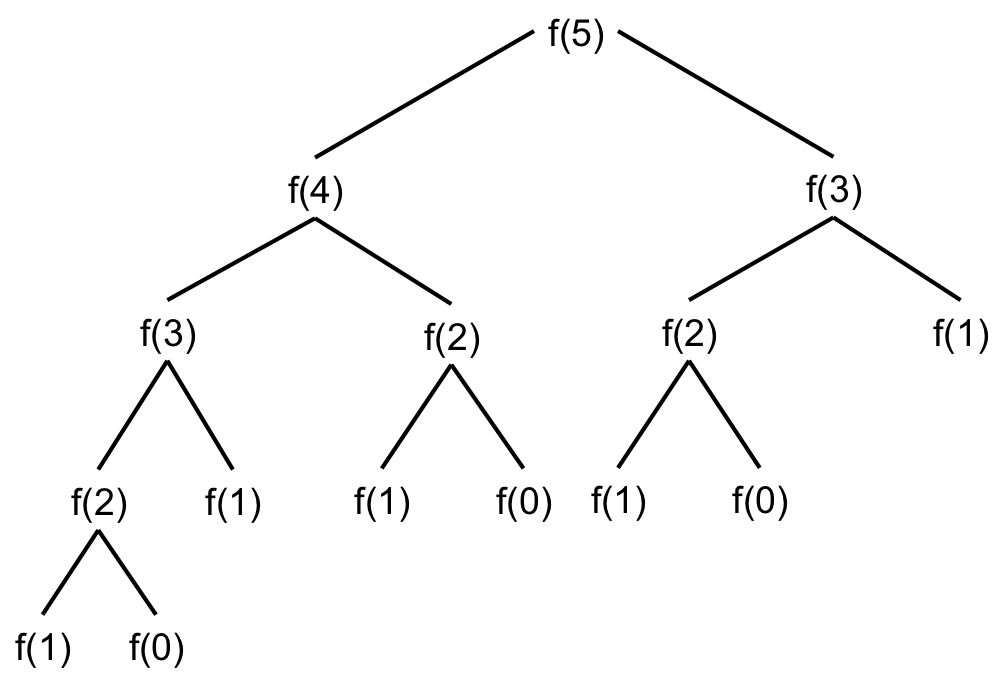
\includegraphics[scale = 0.5]{images/fibonacci_tree.png}
	\caption[Fibonacci Recursion Tree]{Fibonacci Recursion Tree}
	\label{fig:fibonacci_rec}
\end{figure}

Consider the array \texttt{Fibo} which initially contains only $0$'s, and will be used to store the Fibonacci numbers. The recursion function using memoization would look as follows:

\begin{lstlisting}[caption={Fibonacci with Memoization}, label={lst:fibonacci_memoization}, numbers=left]
int f(int n)
{
    if(n == 0 || n == 1)
        return 1;
        
    if(Fibo[n] == 0)
        Fibo[n] = f(n-1) + f(n-2);
    
    return Fibo[n];
}
\end{lstlisting}

In the code showed in \ref{lst:fibonacci_memoization} we notice that we only call the recursive function if the value of \texttt{Fibo[n]} is zero, which means that we have not yet calculated the $n^{th}$ Fibonacci number. Otherwise we return the already calculated value stored in \texttt{Fibo[n]}.


\section{Algorithm Analysis}

The complexity of an algorithm can be defined as how the performance of the algorithm increases as we increase the size of the input data. For example, an algorithm which is efficient to sort ten elements can perform poorly sorting one million elements. 

\subsection{Asymptotic Notations}

When we refer to the running time of an algorithm, we say that it runs in $O(n)$ time, if it has linear complexity, or $O(\log n)$ if it has logarithmic complexity. The $O$ is an asymptotic bound for the running time of an algorithm multiplied by a constant factor, but it is not the only way of describing asymptotic behaviors. Bellow we list three different types of notations used to describe running times of algorithms.

\begin{itemize}
    \item \textbf{$O$-notation.} Used to define an asymptotic upper bound for the running time. Can be used to describe the worst case scenario.
    \item \textbf{$\Omega$-notation.} Define an asymptotic lower bound for the running time of an algorithm. In other words, it is used to describe the best case scenario.
    \item \textbf{$\Theta$-notation.} Specifies both, an asymptotic lower bound, and an asymptotic upper bound for the running time of an algorithm. 
\end{itemize}

Trough the rest of the book we will mostly use the $O$-notation when describing the time complexity of an algorithm. It is important to mention that even when asymptotic notations are commonly associated to the running time, they can also be used to describe other characteristics of the algorithm, such as, memory, for example.\\

There are different kind of algorithms depending on their complexity. Some of the most common belong to the following categories:

\begin{itemize}
    \item \textbf{Constant Complexity.} Their performance does not change with the increase of the input boundaries. We say these algorithms run in $O(1)$ time.
    
    \item \textbf{Linear Complexity.} The performance of these algorithms behaves linearly as we increase the size of the input data. For example, for 1 element, the algorithm executes $k$ operations, for $10$ elements, it makes $10k$ operations, for $100$, it executes $100k$ operations, and so on. We say that these algorithms run in $O(n)$ time.
    
    \item \textbf{Logarithmic Complexity.} The performance increases in a logarithmic way as we increase the data size. Meaning that the if we have 10 elements, the algorithm will execute $\log{10}$ operations, which is around $2.3$. For $1000$ elements, it makes around of $7$ operations, depending on the base of the logarithm. In most of the cases we deal with base-2 logarithms, where:
    $$
    \log_2{n} = \frac{\log n}{\log 2}
    $$
    
    Since $1/\log{2}$ is a multiplicative factor, then we say that these algorithms run in $O(\log n)$ time.
    
    \item \textbf{Polynomial Complexity.} For this kind of algorithms their performance grows in a polynomial rate according to the input data. Some of the most famous sorting algorithms like \textit{Bubble Sort}, run in quadratic time, $O(n^2)$. A well known algorithm that runs in cubic time, $O(n^3)$, is the matrix multiplication. More complex problems have polynomial solutions with greater degree. In programming contests it is common that a problem with an input of $100$ elements still can be solved with a cubic approach, but at the end all depends on the time limits specified by the problem.
    
    \item \textbf{Exponential Complexity.} These are the worst cases and must be avoided if possible, since for a small increment in the input data, their performance grows considerably. There is no doubt that the problems that require exponential solutions, are the hardest ones. We say that these algorithms run in $(a^n)$ time, for some value of $a$.
\end{itemize}



\subsection{Master Theorem}

As we've seen trough this chapter, recursion is a powerful tool that allows us to solve problems that would be impossible to solve with an iterative approach. But one truth about using recursion is that sometimes it is not clear to see at glance what would be the time complexity of an algorithm. For this case, the master theorem specifies three cases that can help us to identify the time complexity of a recursive algorithm.\\

Let $a \geq 1$ and $b \geq 1$ be constants, and let $f(n)$ be a function. If the time complexity, $T(n)$, of a recursive algorithm has the form

$$
T(n) = aT(n/b) + f(n),
$$

where $a$ refers to the number of branches that will came out of the current node in the recursion tree, and $b$ refers to the data size on each of these branches. Then it has the following asymptotic bounds:

\begin{enumerate}
    \item If $f(n) = O(n^{\log_b a - \epsilon})$ for some constant $\epsilon > 0$, then $T(n) = \Theta(n^{\log_b a})$.
    \item If $f(n) = \Theta(n^{\log_b a})$, then $T(n) = \Theta(n^{\log_b a} \log n)$.
    \item If $f(n) = \Omega(n^{\log_b a + \epsilon})$ for some constant $\epsilon > 0$, and if $af(n/b) \leq cf(n)$ for some constant $c < 1$, then for all sufficiently large $n$ we have that $T(n) = \Theta(f(n))$.
\end{enumerate}

When we apply the master theorem, what we do is to compare the function $f(n)$ with the function $n^{\log_b a}$, and to select the larger of the two. If $n^{\log_b a}$ is larger, then we are in the first case, and then $T(n) = \Theta(n^{\log_b a})$. If $f(n)$ is larger, then we are in case 3, and $T(n) = \Theta(f(n))$. If both functions have the same size, then we are in case 2, and we multiply the function by a logarithmic factor, and get $T(n) = \Theta(n^{\log_b a} \log n) = \Theta(f(n) \log n)$.\\

When we say that $f(n)$ must be smaller or larger than  $n^{\log_b a}$, we mean that $f(n)$ must be polynomially smaller or larger than  $n^{\log_b a}$ by a factor of $n^{\epsilon}$, for some $\epsilon > 0$.\\

For a better understanding of the master theorem let's see some examples.

\begin{itemize}
\item $T(n) = T(n/2) + 1$.\\

This example represents a \textit{Binary Search}, which is explained in chapter 5. Here $a = 1, b=2$, and $f(n) = 1$. Then $n^{\log_b a} = n^{\log_2 1} = n^0 = 1$. Since $f(n) = n^{\log_b a} = 1$, then we are in the second case of the master theorem, and $T(n) = \Theta(\log n$).

\item $T(n) = 2T(n/2) + n$.\\

 This case represents the behavior of the \textit{Merge Sort}, which is explained in chapter 3. Here we have $a = 2, b=2$, and $f(n) = n$. Then $n^{\log_b a} = n^{\log_2 2} = n^1 = n$. Since $f(n) = n^{\log_b a}$, again we are in case 2 of the master theorem, and $T(n) = \Theta(n \log n$).
 
 \item $T(n) = 4T(n/2) + n$.\\
 
 For this case we have $a=4, b=2$, and $f(n) = n$. Then $n^{\log_b a} = n^{\log_2 4} = \Theta(n^2)$. Since $f(n) = O(n^{2 - \epsilon})$, with $\epsilon = 1$, then we can apply case 1 of the master theorem and say that $T(n) = \Theta(n^2)$.

\end{itemize}


\subsection{P and NP}

Let's call $P$  the set of problems that can be solved in polynomial time. Let $NP$ be the set of problems whose solution can be verified in polynomial time. Now, it is clear that $P$ is inside $NP$, since a problem which solution can be obtained in polynomial time, can be verified in polynomial time, see figure \ref{fig:p_np}. However is not that clear for the other way around, meaning that a problem whose solution can be verified in polynomial time, it is uncertain that it can be solved in polynomial time. For example, consider the problem of selecting a sub-set of numbers from a given set, in such a way that the sum of the elements in the sub-set is equal to some given number $K$. If a solution is given to us, we can verify in linear time if that solution is correct, just sum all the numbers and check if the result is equal to $K$, but finding that solution seems not that easy.

\begin{figure}[H]
	\centering
	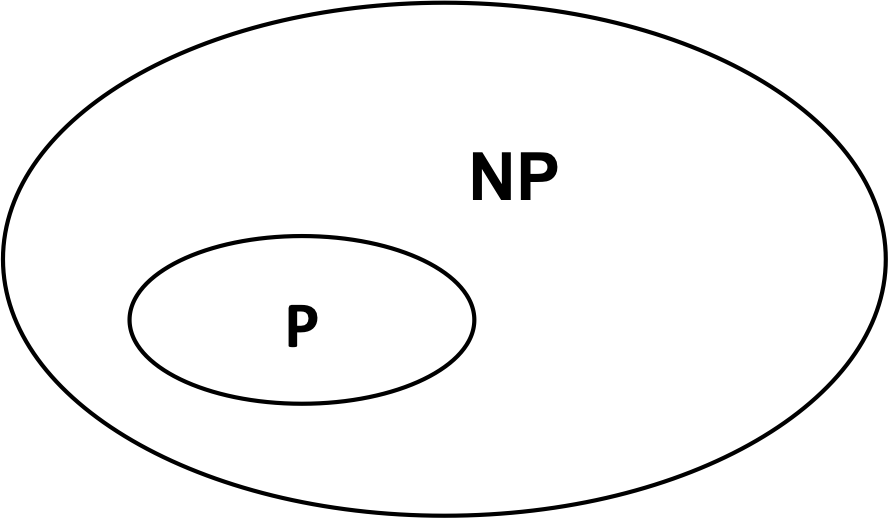
\includegraphics[scale = 0.4]{images/P_NP.png}
	\caption[P and NP]{P and NP problems}
	\label{fig:p_np}
\end{figure}

The proof that a problem whose solution can be easily verified (in polynomial time) can or can't be solved easily (in polynomial time) has not yet found, and it is one of the seven millennium problems.

\section{Bitwise Operations}

Bitwise operations are performed by the processor all the time, because they are the fundamental operations of the computer. Here we will discuss these operations from the programmer perspective, in other words, to make our programs more efficient.\\

These types of operations are executed faster than the arithmetic operations as the sum, multiplication, division or the module, the reason is basically because the arithmetic operations are a set of bitwise operations internally. Therefore whenever we can substitute an arithmetic operation by an bitwise operation we make our program much more faster in terms of execution time.\\

There are a lot of bitwise operators, but in this chapter we will tackle the most important ones.

\subsection{AND (\&) operator}
AND operator is defined as follows:
$0$ \& $0 = 0$, $0$ \& $1 = 0$, $1$ \& $0 = 0$, $1$ \& $1 = 1$. When we have  two numbers formed by several bits each of them, the AND operation is executed in each pair of respective bits. For example, let's take two numbers based on 8 bits, let's say $173 = 10101101$ and $85 = 01010101$, if we make $173$ \& $85$ the result is going to be $5=00000101$, as we can see in the figure 2.3.
\begin{figure}[H]
	\centering
	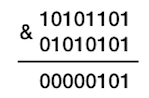
\includegraphics[scale = 0.5]{images/BIT_2.png}
	\caption[AND operator]{Example AND operator}
	\label{fig:bit_2}
\end{figure}
\
An interesting application of this is when we want to know the module $r$ of a number $n$ module $2^m$, because the module $r$ can be obtained by doing $n$ \& $(2^m-1)$. 
For instance, $n=27$ and $m=2$,
$27$ \& $3 = 3$ and $27$ $mod$ $2^2 = 3$. The idea behind this is that $2^m-1$ is a number formed by only 0's at the left and $m$ 1's at the right, so when we make an AND operation the last $m$ bits at the right of $n$ remain as they are and the other ones becomes to 0 and that is exactly the module operation with a power of 2 applied to another number.

\subsection{OR (|) operator}
OR operator is defined as follows:
$0$ | $0 = 0$, $0$ | $1 = 1$, $1$ | $0 = 1$, $1$ | $1 = 1$.

For the case of numbers composed by several bits the OR operation is performed in the same way as the AND operation. For instance, let's take two numbers based on 8 bits, $51 = 00110011$ and $149 = 10010101$, if we make $51$ | $149$ the result is going to be $183=10110111$, as we can see in the figure 2.4.

\begin{figure}[H]
	\centering
	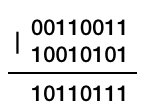
\includegraphics[scale = 0.5]{images/BIT_3.png}
	\caption[OR operator]{Example OR operator}
	\label{fig:bit_3}
\end{figure}
\

To exemplify the utility of this operation, let's imagine that we want to sum integers such that all of them are powers of 2 and they are different from each other. Instead of use the sum operation we can make an OR operation and the outcome will be the wanted, this is because they are powers of 2, therefore they have one bit on and this bit is different from each other, so the OR operator just turn on the respective bit in the result and this is equivalent to the sum operation.

For instance, let's take the numbers $2=00000010$, $8=00001000$ and $32=01000000$, based on 8 bits. The sum is $42=01010010$, which is exactly the same as $00000010$ | $00001000$ | $01000000=01010010=42$.

\subsection{XOR ($\wedge$) operator}
XOR operator is defined as follows: $0\wedge0 = 0$, $0\wedge1 = 1$, $1\wedge0 = 1$, $1\wedge1 = 0$

\subsection{Two's complement}
Two's complement is defined as 

\subsection{Two's complement - 1}
Two's complement - 1 is defined as 


\section{Chapter Notes}

There are a lot of ''famous'' recursion problems, like the \textit{Eight Queens Problem, Sudoku Puzzle}, among others. Some of them are impossible to solve without recursion, or without using other kind of approaches like genetic algorithms, etc. But even when recursion is a powerful technique, we have to be careful when to use it. For the Fibonacci problem mentioned before for example, perhaps recursion here is not the best way to go, unless we use memoization. Even so, a simple array storing all the Fibonacci numbers and a loop cycle would be more than sufficient, and in that way we avoid the problems with memory occasioned by calculating the same Fibonacci number more than once. In few words, we have to choose wisely when to use recursion, as sometimes we don't have a choice, but if we do have a choice, then we have to analyze the cost-benefit factor.\\

In the case of algorithm analysis it is very important to know the basics of it, to have an idea of when an approach will be good or not depending on the input data, and the time and memory limitations. And always keep in mind the worst case scenario when you write a code. The book of \textit{Introduction to Algorithms} \cite{cormen} contains a detailed explanation about this subject.\\

Bit-wise operations are always faster, since they are executed at bit level directly, and there a lot of applications that use them, like communications protocols, and security algorithms. Whenever it is possible it is usually a good idea to use bit-wise operations. Sometimes, they can make the code a little fuzzier because of the symbolic notations, but is worth to try it.

\newpage
\section{Exercises}

\begin{tcolorbox}
\end{tcolorbox}


\chapter{Sorting Algorithms}

\begin{chapquote}{Author's name, \textit{Source of this quote}}
``This is a quote and I don't know who said this.''
\end{chapquote}

\index{sorting} In practice is common to face with the need to sort the data which we are working with to solve a specific problem. Sometimes is necessary and other times it helps to improve the execution time of the program, in any case we are talking about a very important tool in the programming area.\\

In this chapter we will cover some of the most popular sorting algorithms. Depending on the problem, there are algorithms that fit better, some of them are faster in execution time but are more difficult to implement, or sometimes they need a great amount of memory. On the other hand, there are algorithms that perform poorly in execution time, but they are very easy to implement. That's why is important to identify which algorithm is the best for the problem that wants to be solved.\\

Because this book is focused in algorithms for programming contests, and during a contest is important the time it take us to solve a problem, simple algorithms like \textit{Bubble Sort} and \textit {Selection Sort} don't need to be discarded, they can be implemented very fast, and if the number of elements to sort is small, they will work just fine.

\section{Bubble Sort}

Bubble sort \index{bubble sort} is one of the most popular sorting algorithms, is easy to understand and easy to implement. Unfortunately is hard to use it in real-world applications.\\

The algorithm consists in the following. Having an array $X$ with $n$ elements, $x_0, x_1, \ldots, x_{n-1}$. Iterate from $i=0$ to $i=n-2$ comparing element $x_i$ with element $x_{i+1}$, if case $x_i > x_{i+1}$ swap both values.\\

Consider the following array of numbers.\\

\begin{table}[ht]
\centering % used for centering table
\begin{tabular}{|c|c|c|c|c|c|c|c|c|c|}
\hline %inserts double horizontal lines
5 & 3 & 1 & 9 & 0 & 4 & 7 & 2 & 8 & 6 \\
\hline
\end{tabular}
\end{table}

The iterations of the bubble sort method are shown in table \ref{tab:bubble_sort}.

\begin{table}[ht]
\centering % used for centering table
\begin{tabular}{c|c|c|c|c|c|c|c|c|c|c|l}
\hline %inserts double horizontal lines
Iteration 1: & \textbf{5} & \textbf{3} & 1 & 9 & 0 & 4 & 7 & 2 & 8 & 6 & Swap 5 and 3 \\
\hline 
Iteration 2: & 3 & \textbf{5} & \textbf{1} & 9 & 0 & 4 & 7 & 2 & 8 & 6 & Swap 5 and 1 \\
\hline
Iteration 3: & 3 & 1 & \textbf{5} & \textbf{9} & 0 & 4 & 7 & 2 & 8 & 6 & Nothing happens \\
\hline
Iteration 4: & 3 & 1 & 5 & \textbf{9} & \textbf{0} & 4 & 7 & 2 & 8 & 6 & Swap 9 and 0 \\
\hline
Iteration 5: & 3 & 1 & 5 & 0 & \textbf{9} & \textbf{4} & 7 & 2 & 8 & 6 & Swap 9 and 4 \\
\hline
Iteration 6: & 3 & 1 & 5 & 0 & 4 & \textbf{9} & \textbf{7} & 2 & 8 & 6 & Swap 9 and 7 \\
\hline
Iteration 7: & 3 & 1 & 5 & 0 & 4 & 7 & \textbf{9} & \textbf{2} & 8 & 6 & Swap 9 and 2 \\
\hline
Iteration 8: & 3 & 1 & 5 & 0 & 4 & 7 & 2 & \textbf{9} & \textbf{8} & 6 & Swap 9 and 8 \\
\hline
Iteration 9: & 3 & 1 & 5 & 0 & 4 & 7 & 2 & 8 & \textbf{9} & \textbf{6} & Swap 9 and 6 \\
\hline
\end{tabular}
\caption[Bubble Sort]{Iterations of the \textit{Bubble Sort.}}
\label{tab:bubble_sort}
\end{table}

Resulting the following array:

\begin{table}[ht]
\centering % used for centering table
\begin{tabular}{|c|c|c|c|c|c|c|c|c|c|}
\hline %inserts double horizontal lines
3 & 1 & 5 & 0 & 4 & 7 & 2 & 8 & 6 & 9 \\
\hline
\end{tabular}
\end{table}

In \ref{tab:bubble_sort} can be seen that greater values move to the end of the array, meanwhile the smaller ones move to the start of the array.\\

In order to sort the array, the process described above must be repeated at least $n$ times. This to ensure that all elements end in the correct position. The worst case scenario is when the array is initially in decreasing order, because in each iteration the smallest element moves only one position.\\

Program \ref{lst:bubble} read a number $n$ $(1 \leq n \leq 100)$, indicating the number of elements in the array $X$. The next $n$ numbers represents the elements of $X$. The program print the array $X$ with its elements sorted in increasing order.\\

\noindent
\textbf{Time Complexity:} $O(n^2)$ \\
\textbf{Input:}\\
\indent n: Number of elements in the array.\\
\indent X: Array to be sorted.\\
\textbf{Output}:\\
\indent The array $X$ in non-decreasing order.

%\lstset{basicstyle={\small\ttfamily},}
\begin{lstlisting}[caption={Bubble Sort}, label={lst:bubble}, numbers=left]
#include <stdio.h>
#define N 101

int X[N];
int n;
void Bubble_Sort();

int main()
{
    int i;
    scanf("%d", &n);
    
    for(i=0; i<n; i++)
        scanf("%d", &X[i]);
    
    Bubble_Sort();
    
    for(i=0; i<n; i++)
        printf("%d ", X[i]);
    
    printf("\n");
    return 0;
}

void Bubble_Sort()
{
    int i, j;
    int temp;
    
    for(i=0; i<n; i++)
    {
        for(j=0; j<n-1; j++)
        {
            if(X[j] > X[j+1])
            {
                temp = X[j];
                X[j] = X[j+1];
                X[j+1] = temp;
            }
        }
    } 
}
\end{lstlisting}

\section{Selection Sort}

Given an array of $n$ elements, this algorithm \index{selection sort} find the smallest element in an array and place it in the first position, then finds the smallest number from the remaining elements and place it in the second position, and so on, until all elements are sorted.\\

In iteration $i$, the cost of finding the smallest element is $n-i$, because at this point we are sure that the first $i-1$ elements are already sorted. Let's see an example. Consider the following array.

\begin{table}[ht]
\centering % used for centering table
\begin{tabular}{|c|c|c|c|c|c|c|c|c|c|}
\hline %inserts double horizontal lines
5 & 3 & 1 & 9 & 0 & 4 & 7 & 2 & 8 & 6 \\
\hline
\end{tabular}
\end{table}

The iterations of the algorithm are described in table \ref{tab:selection_sort}.

\begin{table}[ht]
\centering % used for centering table
\begin{tabular}{c|c|c|c|c|c|c|c|c|c|c|l}
\hline %inserts double horizontal lines
Iteration 1: & \textbf{5} & 3 & 1 & 9 & \textbf{0} & 4 & 7 & 2 & 8 & 6 & Swap 0 and 5 \\
\hline 
Iteration 2: & \textcolor{red}{0} & \textbf{3} & \textbf{1} & 9 & 5 & 4 & 7 & 2 & 8 & 6 & Swap 3 and 1 \\
\hline 
Iteration 3: & \textcolor{red}{0} & \textcolor{red}{1} & \textbf{3} & 9 & 5 & 4 & 7 & \textbf{2} & 8 & 6 & Swap 3 and 2 \\
\hline 
Iteration 4: & \textcolor{red}{0} & \textcolor{red}{1} & \textcolor{red}{2} & \textbf{9} & 5 & 4 & 7 & \textbf{3} & 8 & 6 & Swap 9 and 3 \\
\hline 
Iteration 5: & \textcolor{red}{0} & \textcolor{red}{1} & \textcolor{red}{2} & \textcolor{red}{3} & \textbf{5} & \textbf{4} & 7 & 9 & 8 & 6 & Swap 5 and 4 \\
\hline 
Iteration 6: & \textcolor{red}{0} & \textcolor{red}{1} & \textcolor{red}{2} & \textcolor{red}{3} & \textcolor{red}{4} & \textbf{5} & 7 & 9 & 8 & 6 & Keep 5 in the same place \\
\hline 
Iteration 7: & \textcolor{red}{0} & \textcolor{red}{1} & \textcolor{red}{2} & \textcolor{red}{3} & \textcolor{red}{4} & \textcolor{red}{5} & \textbf{7} & 9 & 8 & \textbf{6} & Swap 7 and 6 \\
\hline 
Iteration 8: & \textcolor{red}{0} & \textcolor{red}{1} & \textcolor{red}{2} & \textcolor{red}{3} & \textcolor{red}{4} & \textcolor{red}{5} & \textcolor{red}{6} & \textbf{9} & 8 & \textbf{7} & Swap 9 and 7 \\
\hline 
Iteration 9: & \textcolor{red}{0} & \textcolor{red}{1} & \textcolor{red}{2} & \textcolor{red}{3} & \textcolor{red}{4} & \textcolor{red}{5} & \textcolor{red}{6} & \textcolor{red}{7} & 8 & 9 & Array sorted \\
\hline 
\end{tabular}
\caption[Selection Sort]{Iterations of the \textit{Selection Sort.}}
\label{tab:selection_sort}
\end{table}

In \ref{tab:selection_sort} the numbers in red are numbers that are already in correct positions, and the numbers in bold are the ones that need to be swapped.\\

In the first element we need to iterate trough all $n$ elements, for the second one we need to iterate trough $n-1$ elements, and so on. So the number of iterations is given by $n + (n-1) + (n-2) + \cdots + 1 = \frac{n}{2}(n+1)$.\\ 

The code in \ref{lst:selection_sort} reads an integer $n$ $(1 \leq n \leq 100)$. $n$ numbers follow, representing the elements of the array to be sorted. The program print the array sorted in ascending order using the \textit{Selection Sort} algorithm.\\

\noindent
\textbf{Time Complexity:} $O(n^2)$ \\
\textbf{Input:}\\
\indent n: Number of elements in the array.\\
\indent X: Array to be sorted.\\
\textbf{Output}:\\
\indent The array X in non-decreasing order.

\begin{lstlisting}[caption={Selection Sort}, label={lst:selection_sort}, numbers=left]
#include <stdio.h> 
#define N 101

int X[N];
int n;

void Selection_Sort(); 

int main()
{
    int i;

    scanf("%d", &n); 
    
    for(i=0; i<n; i++)
        scanf("%d", &X[i]);
    
    Selection_Sort();

    for(i=0; i<n; i++) 
        printf("%d ", X[i]);
    
    printf("\n");
    return 0;
}

void Selection_Sort() 
{
    int i, j, pos, temp;
    
    for(i=0; i<n-1; i++) 
    {
        pos = i;
        for(j=i+1; j<n; j++) 
        {
            if(X[j] < X[pos])
                pos = j;
        }
        
        temp = X[i];
        X[i] = X[pos];
        X[pos] = temp;
    } 
}
\end{lstlisting}

\section{Insertion Sort}

To explain this method \index{insertion sort} imagine we have an array of $i$ elements sorted and we want to add a new element. To keep the array sorted we need to place the new element in the correct position. On each iteration from $i=1$ to $i=n-1$ we add a new member to the current sorted array of $i$ elements. To do that, all the elements greater than the new element must be shifted to the right in order to make space to the new element. Consider the following array:\\

\begin{table}[ht]
\centering % used for centering table
\begin{tabular}{|c|c|c|c|c|}
\hline %inserts double horizontal lines
1 & 3 & 6 & 7 & 10 \\
\hline
\end{tabular}
\end{table}

To add a new element with a value of 5, we must shift to the right the elements greater than 5, and place the new element in the correct position.\\

\begin{table}[ht]
\centering % used for centering table
\begin{tabular}{|c|c|c|c|c|c|}
\hline %inserts double horizontal lines
1 & 3 & \textcolor{red}{5} & 6 & 7 & 10 \\
\hline
\end{tabular}
\end{table}

In the worst case the elements are given in descending order, making in each iteration to shift all the elements in the array. The program in \ref{lst:insertion_sort} reads an integer $n$ $(1 \leq n \leq 100)$, indicating the number of elements in the array. Next $n$ numbers represent the elements in the array. The program uses \textit{Insertion Sort} to print the given array in ascending order.\\ 

\noindent 
\textbf{Time Complexity:} $O(n^2)$ \\
\textbf{Input:}\\
\indent n: Number of elements in the array.\\
\indent X: Array to be sorted.\\
\textbf{Output}:\\
\indent The array X with its elements in non-decreasing order.

\begin{lstlisting}[caption={Insertion Sort}, label={lst:insertion_sort}, numbers=left]
#include <stdio.h> 
#define N 101

int X[N];
int n;

int main() 
{
    int i, j, aux; 
    
    scanf("%d", &n);

    for(i=0; i<n; i++)
    {
        scanf("%d", &X[i]); 
        j = i;
        aux = X[i];
        while(j > 0 && aux < X[j-1]) 
        {
            X[j] = X[j-1];
            j--; 
        }
        
        X[j] = aux; 
    }

    for(i=0; i<n; i++) 
        printf("%d ", X[i]);
    printf("\n");
    return 0;
}
\end{lstlisting}

\section{Counting Sort}

This algorithm \index{counting sort} is very useful when we are handling a big amount of data, but is recommended to use it only when the data can be expressed as non-negative integer numbers in a small interval. The main idea is to count occurrences in terms of the numerical value, for example, consider the following group of integers in the interval $[0, 9]$:

\begin{center}
$0,0,1,3,5,3,2,1,0,1,3,7,8,2,1,3,5,6,5,3$
\end{center}

For this case we have three 0’s, four 1’s, two 2’s, five 3’s, zero 4’s, three 5’s, one 6, one 7, one 8 and zero 9’s. Then, we only need to store the occurrences in a vector $C$ of size equal to the biggest element in the data, where $C_k$ represents the number of occurrences of element $k$. The vector $C$ for this example looks as follows:

\begin{table}[ht]
\centering % used for centering table
\begin{tabular}{|c|c|c|c|c|c|c|c|c|c|c|}
\hline %inserts double horizontal lines
& 0 & 1 & 2 & 3 & 4 & 5 & 6 & 7 & 8 & 9 \\ [0.5ex]
% inserts table
%heading
\hline % inserts single horizontal line
$C=$ & 3 & 4 & 2 & 5 & 0 & 3 & 1 & 1 & 1 & 0 \\
\hline %inserts single line
\end{tabular}
%\caption{Counting Sort example} % title of Table
%\label{table:nonlin} % is used to refer this table in the text
\end{table}

The program in \ref{lst:counting_sort} receives a number $n$, indicating the amount of elements to be sorted. $n$ numbers follow, each one in the interval $[0,9]$. The output is the numbers from the input sorted in ascending order.\\

\noindent \textbf{Time Complexity:} $O(n)$\\
\textbf{Input:}\\
\indent n: Number of elements in the array.\\
\indent num: Elements to be sorted.\\
\textbf{Output}:\\
\indent The array sorted.

\begin{lstlisting}[caption={Counting Sort}, label={lst:counting_sort}, numbers=left]
#include <stdio.h> 
#define N 10

int C[N];
int n;

int main() 
{
    int i, j, num; 
    
    scanf("%d", &n);

    for(i=0; i<n; i++) 
    {
        scanf("%d", &num);
        C[num]++; 
    }

    for(i=0; i<N; i++) 
        for(j=0; j<C[i]; j++)
            printf("%d ", i);
    
    printf("\n");
    return 0; 
}
\end{lstlisting}

\section{Quick Sort}

This algorithm \index{quick sort} was discovered by Antony Richard Hoare \cite{quicksort} at the end of the 50's and begin of the 60's. Many libraries of some programming languages use this algorithm because its time and memory complexity are very efficient in the most cases. 
The main idea behind this algorithm is to place an element called \textit{pivot} in a position where the elements at its left are smaller and the elements at its right are bigger or equal.\\

\begin{algorithm}
\caption{$quicksort(a,b)$}
\begin{algorithmic}
    \STATE $X_{pivot} = X_b$
    \STATE $i \gets a$
    \STATE $j \gets b-1$
    \WHILE{$i \geq j$}
        \IF{$X_i < X_{pivot}$}
            \STATE $i \gets i+1$
        \ELSIF{$X_j \geq X_{pivot}$}
            \STATE $j \gets j-1$
        \ELSIF{$X_i > X_{pivot}$ and $X_j < X_{pivot}$}
            \STATE $swap(X_i,X_j)$
            \STATE $i \gets i+1$
            \STATE $j \gets j-1$
        \ENDIF
    \ENDWHILE
    \STATE $swap(X_i,X_{pivot})$
    \STATE $quicksort(a,i-1)$
    \STATE $quicksort(i+1,b)$
\end{algorithmic}
\label{alg:quick_sort}
\end{algorithm}

We consider an array $x_{0}$, $x_{1}$, $x_{2}$, ... , $x_{n-1}$.   If we take the last element, $x_{n-1}$, as the pivot. Place an iterator $i$ at position 0, and another iterator $j$ at position $n-2$. If $x_i$ is smaller than the pivot, increase $i$ in one. Also if $x_j$ is greater or equal than the pivot, decrease $j$ in one. In the case that $x_i$ is greater or equal than the pivot and that $x_j$ is smaller than the pivot, swap both elements and continue. The process stops when $i$ is greater than $j$. At the end just swap $x_i$ and the pivot. This will ensure that the pivot is in the correct position. Repeat the process with the sub-array in the left side of the pivot and with the sub-array in the right side of the pivot. At the end, the whole array will be sorted. The \textit{Quick Sort} algorithm to sort an array $X$ from position $a$ to position $b$ is showed in algorithm \ref{alg:quick_sort}.\\

The worst case scenario is when all elements are sorted in non-ascending order, because for all the elements will be located in the right side of the pivot in each iteration, for the first pivot there will be $n-1$ elements at its right, for the next pivot there will be $n-2$, and so on, in order to avoid this, many algorithms run a random sort algorithm before execute quicksort reaching $O(nlogn)$ most of the times.\\

The code in \ref{lst:quick_sort} implements \textit{Quick Sort} to sort an array $X$ of $n$ elements $(1 \leq n < 20)$. The input consists of number $n$, and the $n$ numbers that form $X$. The output is $X$ with its elements sorted in ascending order.\\

\noindent \textbf{Time Complexity:} $O(n^2)$, \\
It's important to say that there are many inputs where the time complexity of this algorithm is $O(nlogn)$, and that's why is widely used.\\
\textbf{Input:}\\
\indent n: The number of elements in the array.\\
\indent X: Array to be sorted.\\
\textbf{Output}:\\
\indent The array sorted.

\begin{lstlisting}[caption={Quick Sort}, label={lst:quick_sort}, numbers=left]
#include <stdio.h>

int X[20];
int n;

void Quicksort(int, int);
int Get_Pivot(int, int);
void Swap(int, int);

int main()
{
    int i;
    
    scanf("%d", &n);
    for(i=0; i<n; i++)
        scanf("%d", &X[i]);
    
    Quicksort(0,n-1);
    
    for(i=0; i<n; i++)
        printf("%d ", X[i]);
    
    printf("\n");
    return 0;
}
\end{lstlisting}

The function \texttt{Quicksort} defined bellow, receives two integers that corresponds to the interval to be sorted. Using the pivot it call itself to sort the sub-interval at the left of the pivot and the sub-interval at the right od the pivot.

\begin{lstlisting}[numbers=left]
void Quicksort(int a, int b)
{
    int p;
    if(a < b)
    {
        p = Get_Pivot(a,b);
        Quicksort(a,p-1);
        Quicksort(p+1,b);
    }
}
\end{lstlisting}

The key part in the \textit{Quick Sort} algorithm consists on placing in the right position the pivot. The function \texttt{Get\_Pivot} place the pivot in the correct position in the interval $[a,b]$ according to the algorithm described before. 

\begin{lstlisting}[numbers=left]
int Get_Pivot(int a, int b)
{
    int i = a;
    int j = b-1;
    int p = b;
    while(i <= j)
    {
        if(X[i] < X[p])
            i++;
        else if(X[j] >= X[p])
            j--;
        else if(X[i] >= X[p] && X[j] < X[p])
            Swap(i++,j--);
    }
    
    Swap(i,p);
    return i;
}
\end{lstlisting}

The \texttt{Swap} function receives to integers $i$ and $j$ and swap the elements $X_i$ and $X_j$ in the array.

\begin{lstlisting}[numbers=left]
void Swap(int i, int j)
{
    int temp;
    temp = X[i];
    X[i] = X[j];
    X[j] = temp;
}
\end{lstlisting}

\section{Merge Sort}

Suppose we want to sort the elements of a vector X in non-decreasing order from positions $a$ to $b$. This algorithm \index{merge sort} consists of four steps:

\begin{enumerate}
\item Divide the vector in two parts by finding the middle value $X_m$, where $m = (a+ b)/2$.
\item Sort the elements in the left side.
\item Sort the elements in the right side.
\item Combine the elements in the left side with the elements in the right side in such a way
that the resulting vector is sorted.
\end{enumerate}

Step 4 is the most important. Figure \ref{fig:merge_process} shows the merge process of array $A$ and array $B$ into an array $C$, where $A$ and $B$ are sorted in non-decreasing order. Basically the idea of the merging process consists on placing an iterator $i$ (red) at the beginning of array $A$, and an iterator $j$ (blue) at the beginning of array $B$. If $A_i < B_j$ the element $A_i$ is inserted at the end of array $C$ and $i$ is moved to the next position. Otherwise if $A_i \geq B_j$, element $B_j$ is inserted at the end of $C$ and $j$ is moved to the next position. The process continues until all the elements of either $A$ or $B$ are inserted into $C$.  

\begin{figure}[H]
    \centering
    \subfloat [Iteration 1] 
    {
        \label{fig:merge_process_1} 
        $\begin{aligned}
            A &= [\textcolor{red}{0},2,5,9,10] \\
            B &= [\textcolor{blue}{1},6,7,12,16]\\
            C &= [0]
        \end{aligned}$
    } \qquad
    \subfloat [Iteration 2] 
    {
        \label{fig:merge_process_2}
         $\begin{aligned}
            A &= [0,\textcolor{red}{2},5,9,10] \\
            B &= [\textcolor{blue}{1},6,7,12,16]\\
            C &= [0,1]
        \end{aligned}$ 
    } \qquad
     \subfloat [Iteration 3] 
    {
        \label{fig:merge_process_3}
         $\begin{aligned}
            A &= [0,\textcolor{red}{2},5,9,10] \\
            B &= [1,\textcolor{blue}{6},7,12,16]\\
            C &= [0,1,2]
        \end{aligned}$ 
    } \\
    \subfloat [Iteration 4] 
    {
        \label{fig:merge_process_4} 
        $\begin{aligned}
            A &= [0,2,\textcolor{red}{5},9,10] \\
            B &= [1,\textcolor{blue}{6},7,12,16]\\
            C &= [0,1,2,5]
        \end{aligned}$
    } \qquad
    \subfloat [Iteration 5] 
    {
        \label{fig:merge_process_5}
         $\begin{aligned}
            A &= [0,2,5,\textcolor{red}{9},10] \\
            B &= [1,\textcolor{blue}{6},7,12,16]\\
            C &= [0,1,2,5,6]
        \end{aligned}$ 
    } \qquad
     \subfloat [Iteration 6] 
    {
        \label{fig:merge_process_6}
         $\begin{aligned}
            A &= [0,2,5,\textcolor{red}{9},10] \\
            B &= [1,6,\textcolor{blue}{7},12,16]\\
            C &= [0,1,2,5,6,7]
        \end{aligned}$ 
    } \\
    \subfloat [Iteration 7] 
    {
        \label{fig:merge_process_7} 
        $\begin{aligned}
            A &= [0,2,5,\textcolor{red}{9},10] \\
            B &= [1,6,7,\textcolor{blue}{12},16]\\
            C &= [0,1,2,5,6,7,9]
        \end{aligned}$
    } \qquad
    \subfloat [Iteration 8] 
    {
        \label{fig:merge_process_8}
         $\begin{aligned}
            A &= [0,2,5,9,\textcolor{red}{10}] \\
            B &= [1,6,7,\textcolor{blue}{12},16]\\
            C &= [0,1,2,5,6,7,9,10]
        \end{aligned}$ 
    } \\
\caption[Merge Sort]{Iterations of the merge process of two arrays previously sorted}
\label{fig:merge_process}
\end{figure}

Once one of the iterators reach the end of the array, we just add to $C$ the remaining elements of the other array. Now $C$ contains all the elements of $A$ and $C$ in non-decreasing order.

$$
C = [0,1,2,5,6,7,9,10,12,16]
$$

At the beginning there are $n$ elements in the array, then it is split in two halves of $n/2$ elements each, and each half is divided again in two halves of $n/4$ elements, and so on. Then the execution time depends on how many times we divide the array. We know that we cannot divide the array if there is only one element, this is when $n/2^k = 1$. Solving for $k$, we have that $k = \log_2 n$, and each time we need to perform the merge process, so the time complexity of the \textit{Merge Sort} is $O(n \log n)$.\\

The program \ref{lst:merge_sort} receives and integer $n$ $(1 \leq n \leq 100)$ representing the number of elements in the array $X$. The next $n$ numbers are the elements of $X$. The output is the array $X$ sorted using the \textit{Merge Sort} algorithm.\\

\noindent \textbf{Time Complexity:} $O(n\log n)$\\
\textbf{Input:}\\
\indent n: The number of elements in the array.\\
\indent X: Array to be sorted.\\
\textbf{Output}:\\
\indent The array sorted.

\begin{lstlisting}[caption={Merge Sort}, label={lst:merge_sort}, numbers=left]
#include <stdio.h> 
#define N 101

int X[N], C[N];
int n;

void mergesort(int, int); 
void merge(int, int, int);

int main() 
{
    int i;
    scanf("%d", &n);
    
    for(i=0; i<n; i++) 
        scanf("%d", &X[i]);

    mergesort(0,n-1);

    for(i=0; i<n; i++) 
        printf("%d ", X[i]);

    printf("\n");
    return 0;
}
\end{lstlisting}

The function \texttt{mergesort} receives an interval of the elements to sort, calculates the middle element, and recursively call itself again to sort both halves of the interval. Finally both halves are merged sorting all the elements in the interval.

\begin{lstlisting}[numbers=left]
void mergesort(int i, int j) 
{
    int m;
    
    if(i != j)
    {
        m = (i + j)/2;
        mergesort(i,m);
        mergesort(m+1, j); 
        merge(i, m, j);
    }
}
\end{lstlisting}

The merge process explained before takes place in the \texttt{merge} function, which receives the indexes $i$ and $j$ of the interval to sort, and the middle point, and sort both halves of the array.

\begin{lstlisting}[numbers=left]
void merge(int i, int m, int j) 
{
    int p, q, r;
    
    p = i;
    q = m+1;
    r = i;
    
    while(p <= m && q <= j) 
    {
        if(X[p] <= X[q])
            C[r++] = X[p++];
        else
            C[r++] = X[q++];
    }
    
    while(p <= m)
        C[r++] = X[p++];
    
    while(q <= j)
        C[r++] = X[q++];

    for(r=i; r<=j; r++) 
        X[r] = C[r];
}
\end{lstlisting}

\section{Heap Sort}

The \textit{Heap Sort} \index{heap sort} algorithm was invented by Joseph Williams in 1964. \cite{heapsort}. The main idea of this algorithm is to store the elements of a vector in a heap. A heap \index{heap} is a binary tree where the value of a node is greater or equal than the value of its children. If the value of a node is smaller than the value of one of its children, then the node is swapped with the children with greater value.\\

\begin{figure}[H]
	\centering
	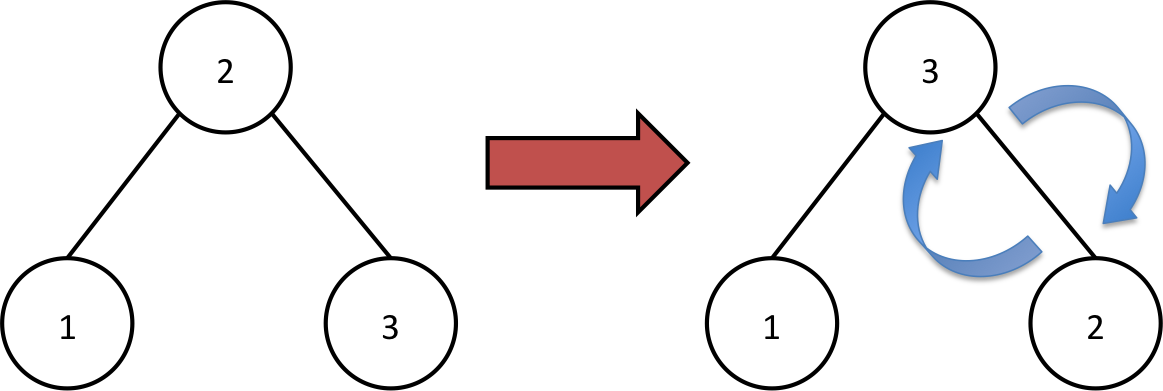
\includegraphics[scale = 0.3]{images/heapSort1.png}
	\caption[Heap Sort. Swap]{Swapping process in heap sort}
	\label{fig:heapsort1}
\end{figure}

Let's explain how to implement a binary tree in an array. Suppose we have a parent node in the position $i$ then the left child would be in the position $2i+1$ and the right child in the position $2i+2$. For instance the root would be at index 0, its left child at index 1 and its right child at index 2, now the child of the node located at index 1 would be at index 3 and the right child at index 4, for the node placed at index 2 the left child would be at index 5 and the right child at index 6, by doing this process we obtain the entire binary tree.\\
\newline
Consider the following sequence of numbers:

\begin{table}[ht]
\centering % used for centering table
\begin{tabular}{c|c|c|c|c|c|c|c|c|c|c}
\hline %inserts double horizontal lines
& X[0] & X[1] & X[2] & X[3] & X[4] & X[5] & X[6] & X[7] & X[8] & X[9] \\ [0.5ex]
\hline % inserts single horizontal line
$X=$ & 2 & 1 & 4 & 6 & 3 & 0 & 7 & 9 & 8 & 5 \\
\hline %inserts single line
\end{tabular}
\end{table}

The heap can be constructed in different ways. One option is to store all elements in a tree like in \ref{fig:heapsort2_1}, and then starting from the last element to the first, swap each element the times it is necessary until it reaches a valid position, the result of doing this is showed in \ref{fig:heapsort2_2}.\\

Another option to build a heap consists on placing the elements in the correct position of the heap  at the same time we are reading the numbers.That could led us to a different heap, but a valid one.\\

We can use any method to build the heap, as long as we don't break the rule that a node must be greater or equal that its children.

\begin{figure}[H]	
	\centering
	\subfloat [Vector $X$ in a tree structure before swaps (not heap)] {\label{fig:heapsort2_1}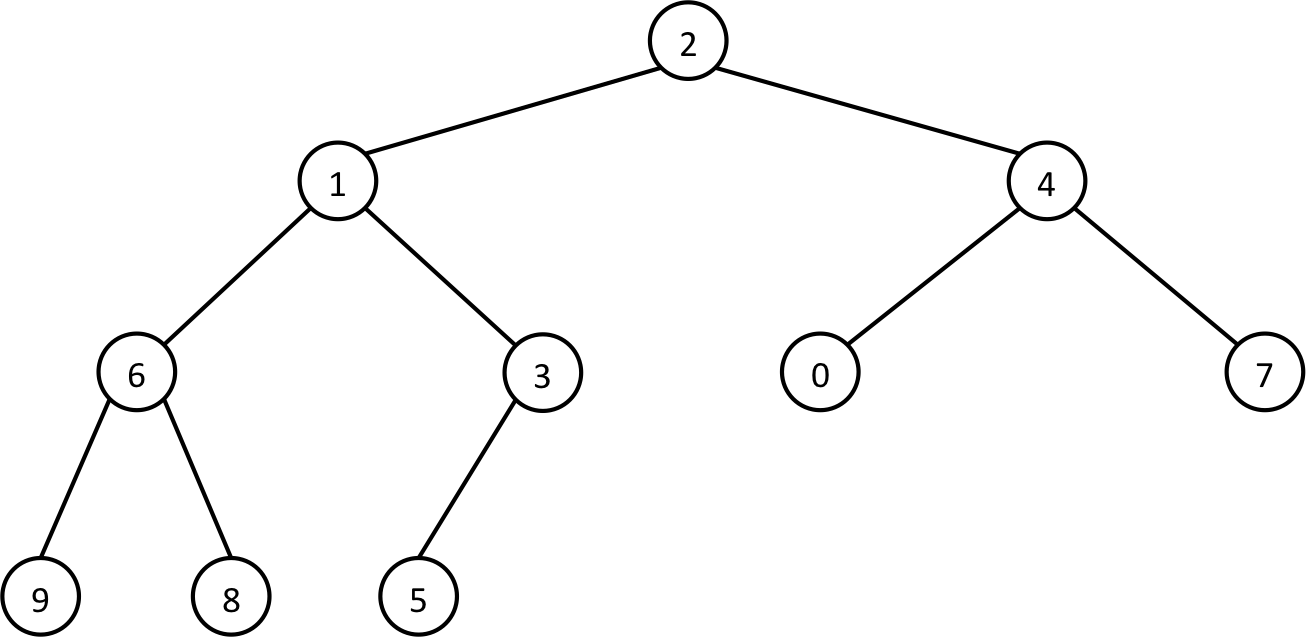
\includegraphics[scale=0.25, clip]{images/heapSort2.png}} \ \ \
	\subfloat [Vector $X$ in a heap structure after swaps] {\label{fig:heapsort2_2} 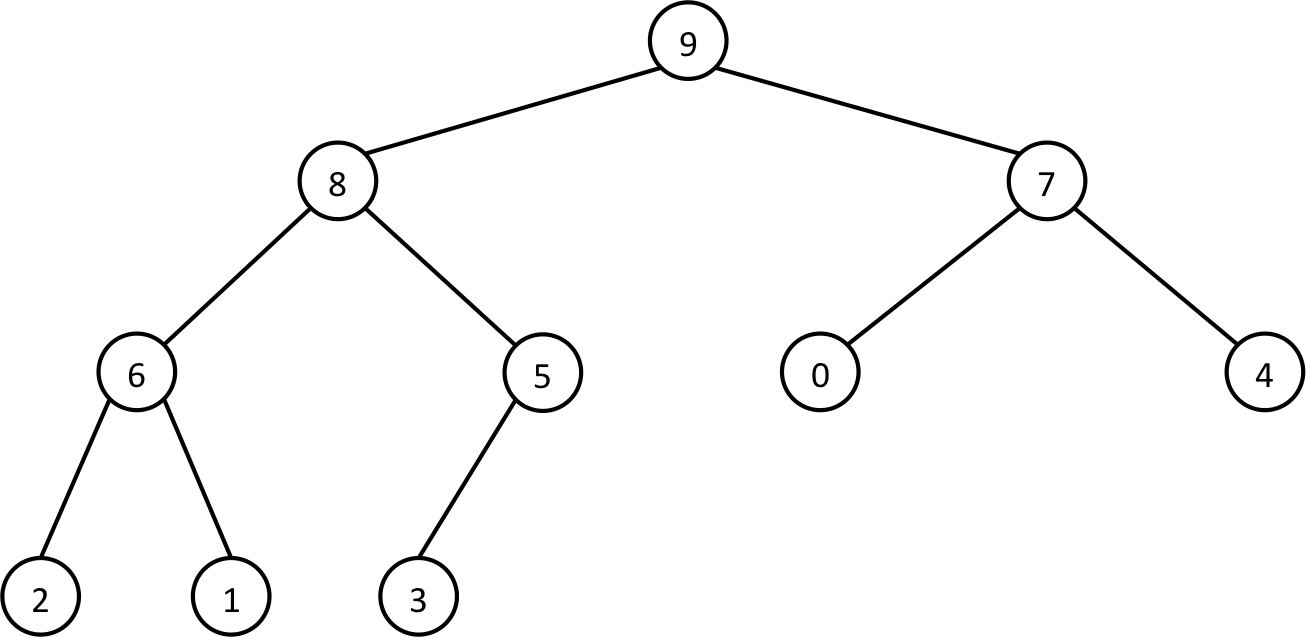
\includegraphics[scale=0.25, clip]{images/heapSort3.png}}\\
	\caption[Heap Sort. Building a heap]{Building a heap sort with the input data. A node is greater or equal than its children.}
	\label{fig:heapsort2}
\end{figure}

 The array representation for the heap in \ref{fig:heapsort2_2} is the following:

\begin{table}[H]
\centering % used for centering table
\begin{tabular}{c|c|c|c|c|c|c|c|c|c|c}
\hline %inserts double horizontal lines
& X[0] & X[1] & X[2] & X[3] & X[4] & X[5] & X[6] & X[7] & X[8] & X[9] \\ [0.5ex]
\hline % inserts single horizontal line
$X=$ & 9 & 8 & 7 & 6 & 5 & 0 & 4 & 2 & 1 & 3 \\
\hline %inserts single line
\end{tabular}
\caption[Heap representation with an array]{Heap represented with an array}
\label{table:heap_array}
\end{table}

The next step is to swap the first element of $X$ (root node) with the last element. Then remove the last element from the heap because it is already in the right position of the array, and move the root element to the correct position using swapping operations. This will convert the tree into a heap again. Continue doing this until all elements in the heap have been removed. Figure \ref{fig:heapsort3} shows the different iterations of the \textit{Heap Sort}.

\begin{figure}[H]	
	\centering
	\subfloat [Swap nodes 3 and 9, and rearrange the heap with the remaining nodes.] {\label{fig:heapsort3_1}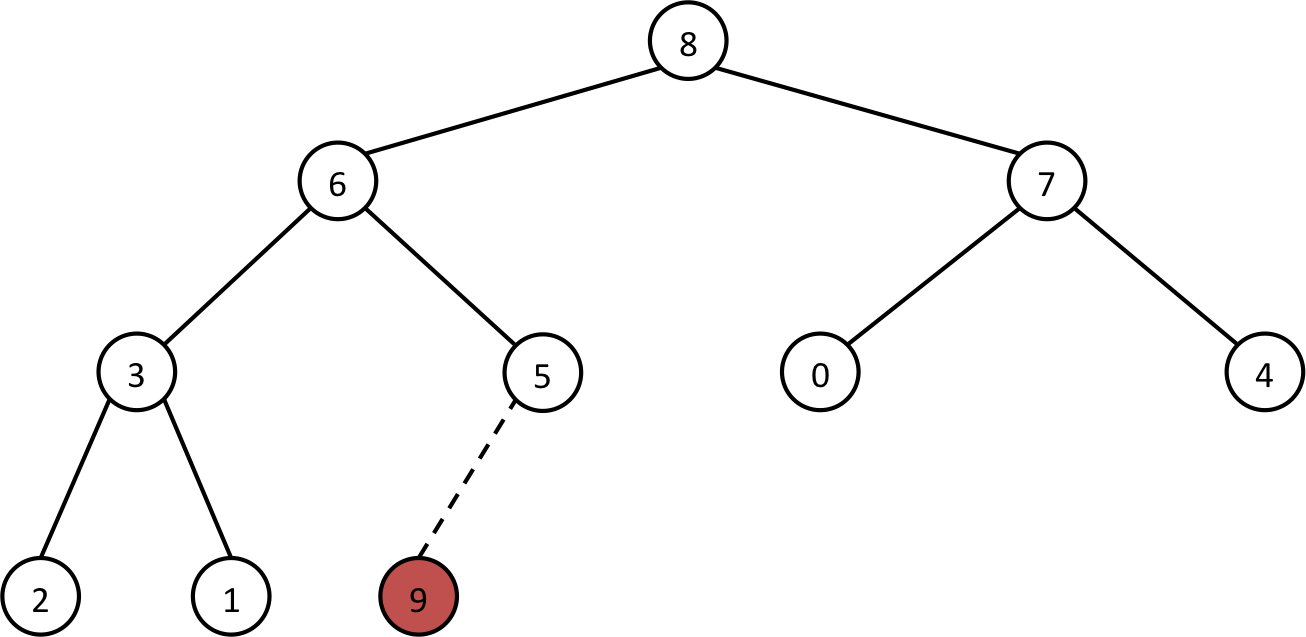
\includegraphics[scale=0.25, clip]{images/heapSort5.png}} \ \ \
	\subfloat [Swap nodes 1 and 8, and rearrange the heap with the remaining nodes] {\label{fig:heapsort3_2} 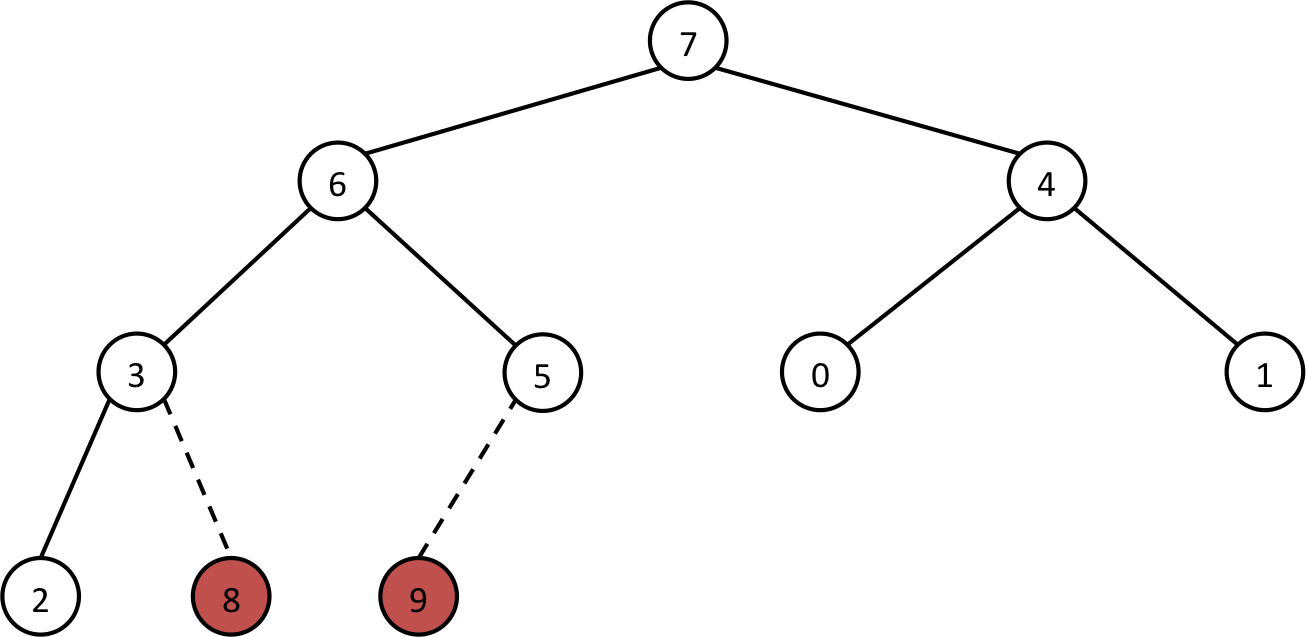
\includegraphics[scale=0.25, clip]{images/heapSort6.png}}\\
\end{figure}
\begin{figure}[H]	
	\centering
	\subfloat [Swap nodes 2 and 7, and rearrange the heap with the remaining nodes.] {\label{fig:heapsort3_3}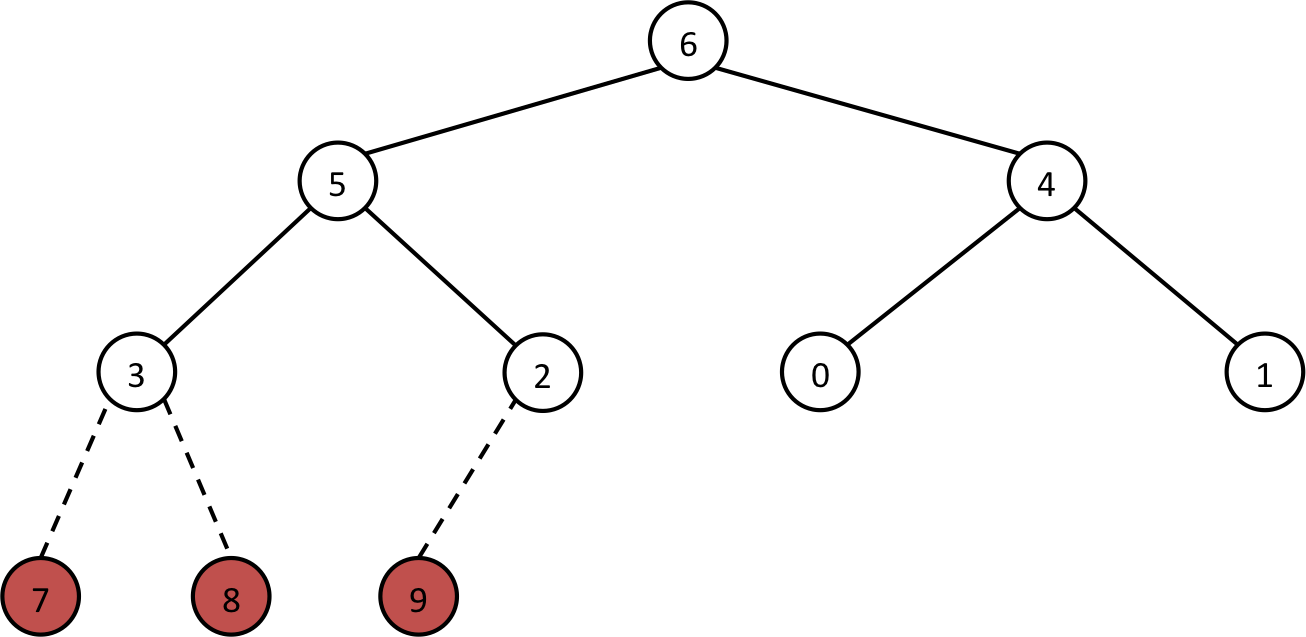
\includegraphics[scale=0.25, clip]{images/heapSort7.png}} \ \ \
	\subfloat [Swap nodes 1 and 6, and rearrange the heap with the remaining nodes] {\label{fig:heapsort3_4} 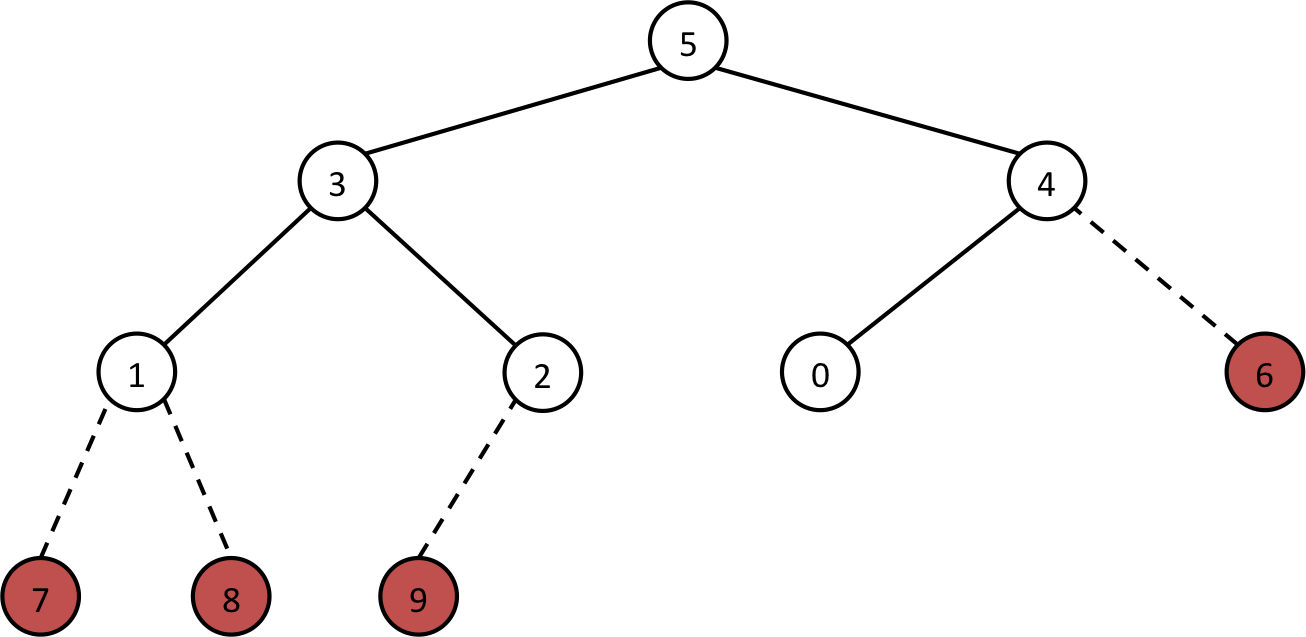
\includegraphics[scale=0.25, clip]{images/heapSort8.png}}\\
\end{figure}
\begin{figure}[H]	
	\centering
	\subfloat [Swap nodes 0 and 5, and rearrange the heap with the remaining nodes.] {\label{fig:heapsort3_5}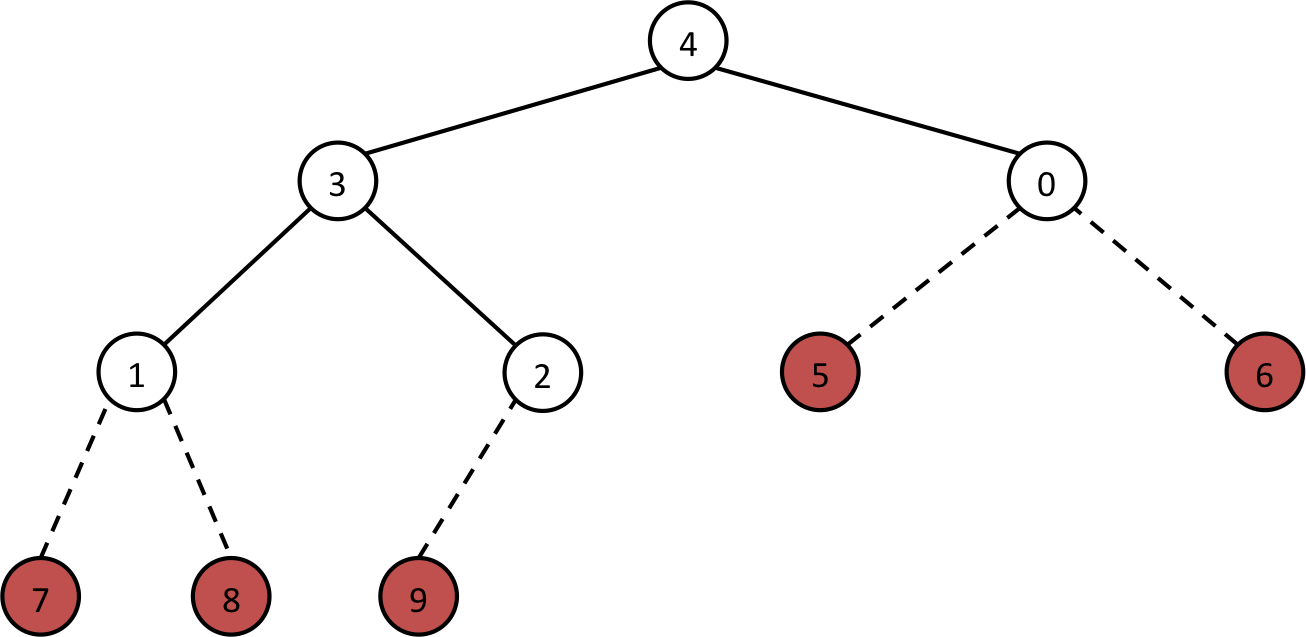
\includegraphics[scale=0.25, clip]{images/heapSort9.png}} \ \ \
	\subfloat [Swap nodes 2 and 4, and rearrange the heap with the remaining nodes.] {\label{fig:heapsort3_6} 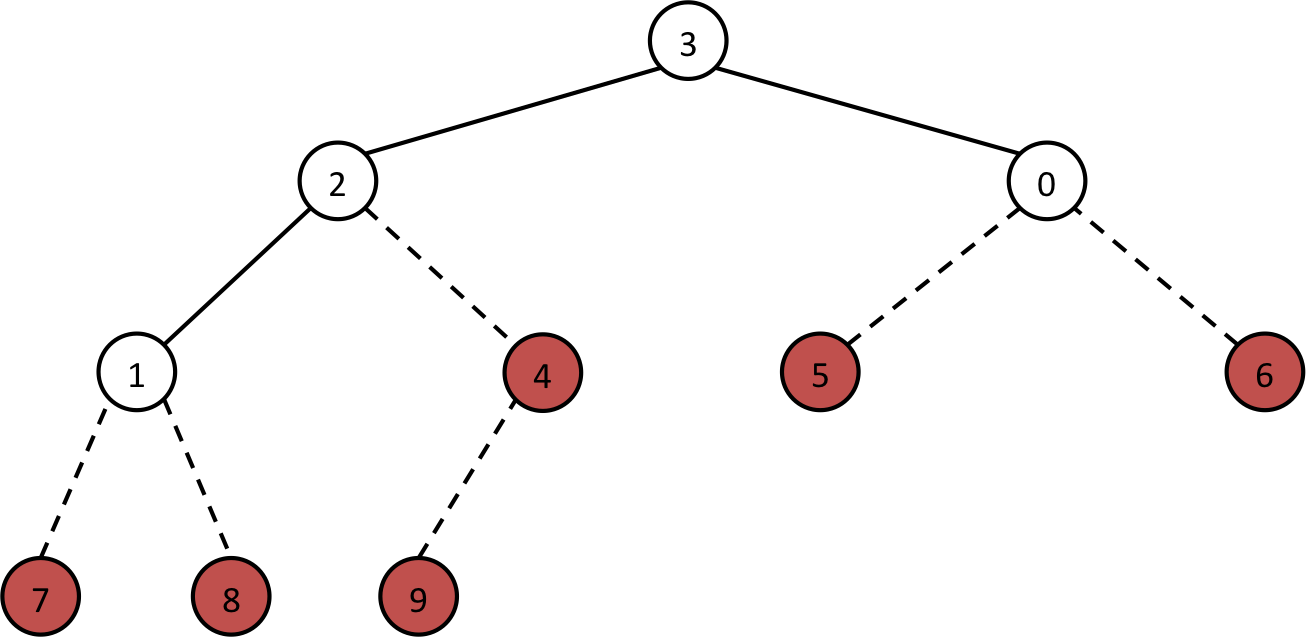
\includegraphics[scale=0.25, clip]{images/heapSort10.png}}\\
\end{figure}
\begin{figure}[H]	
	\centering
	\subfloat [Swap nodes 1 and 3, and rearrange the heap with the remaining nodes.] {\label{fig:heapsort3_7}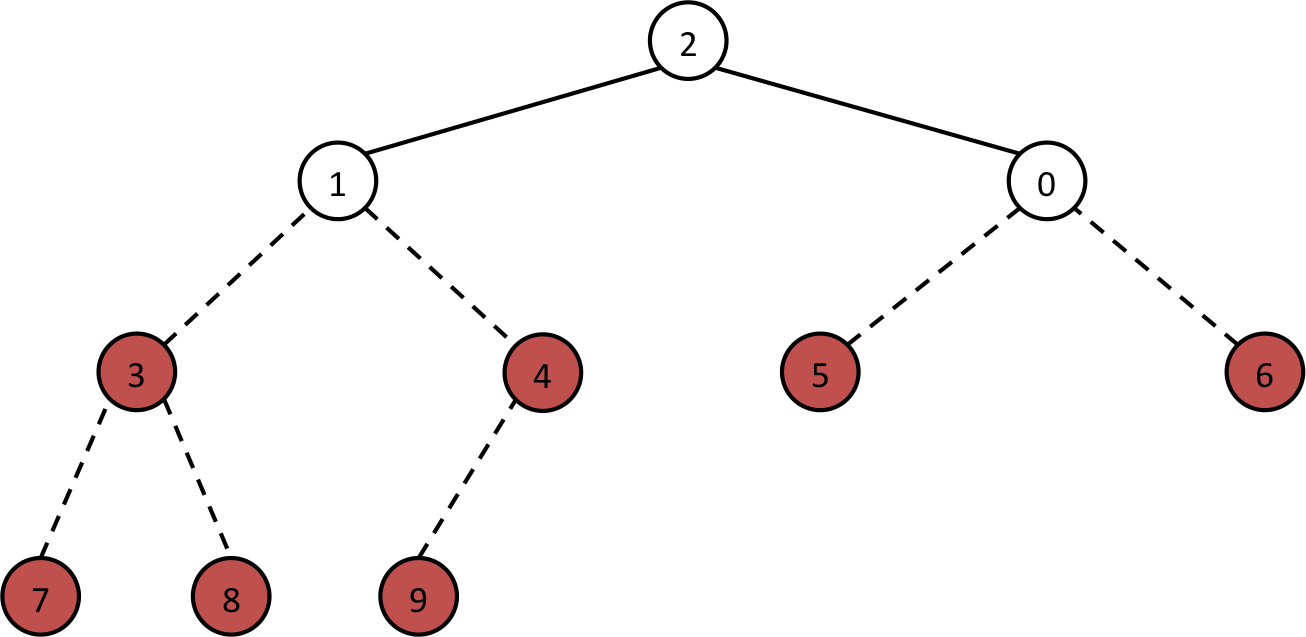
\includegraphics[scale=0.25, clip]{images/heapSort11.png}} \ \ \
	\subfloat [Swap nodes 0 and 2, and rearrange the heap with the remaining nodes.] {\label{fig:heapsort3_8} 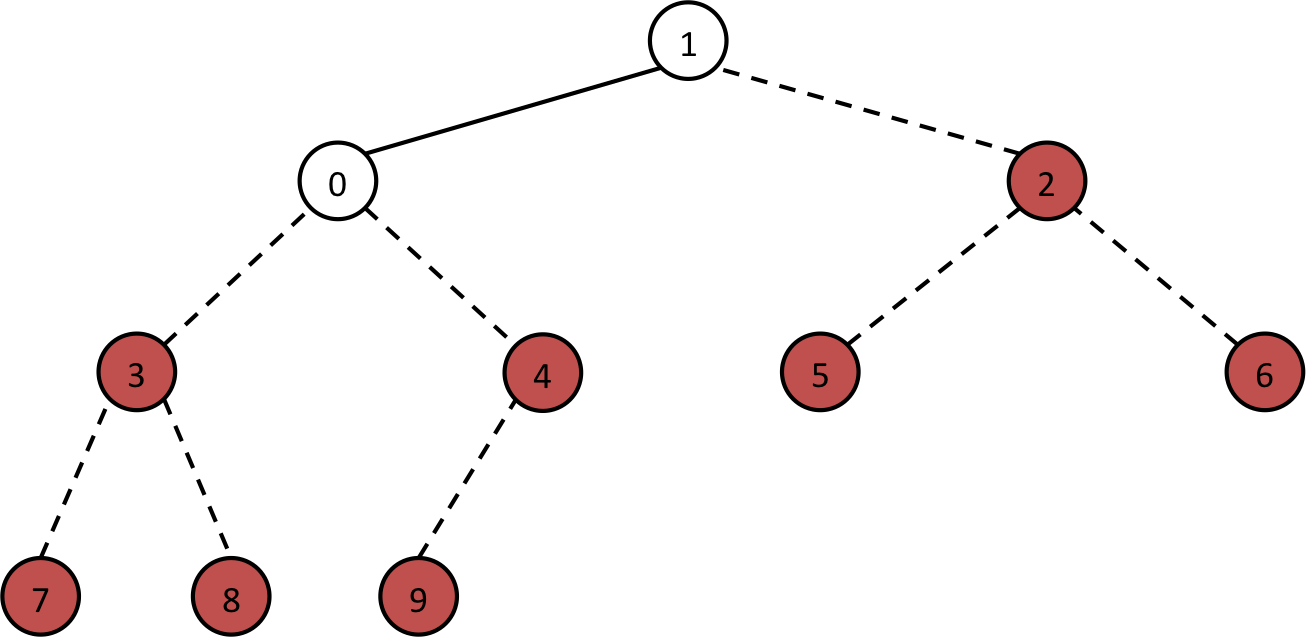
\includegraphics[scale=0.25, clip]{images/heapSort12.png}}\\
\end{figure}
\begin{figure}[H]	
	\centering
	\subfloat [Swap nodes 0 and 1, and rearrange the heap with the remaining nodes.] {\label{fig:heapsort3_9} 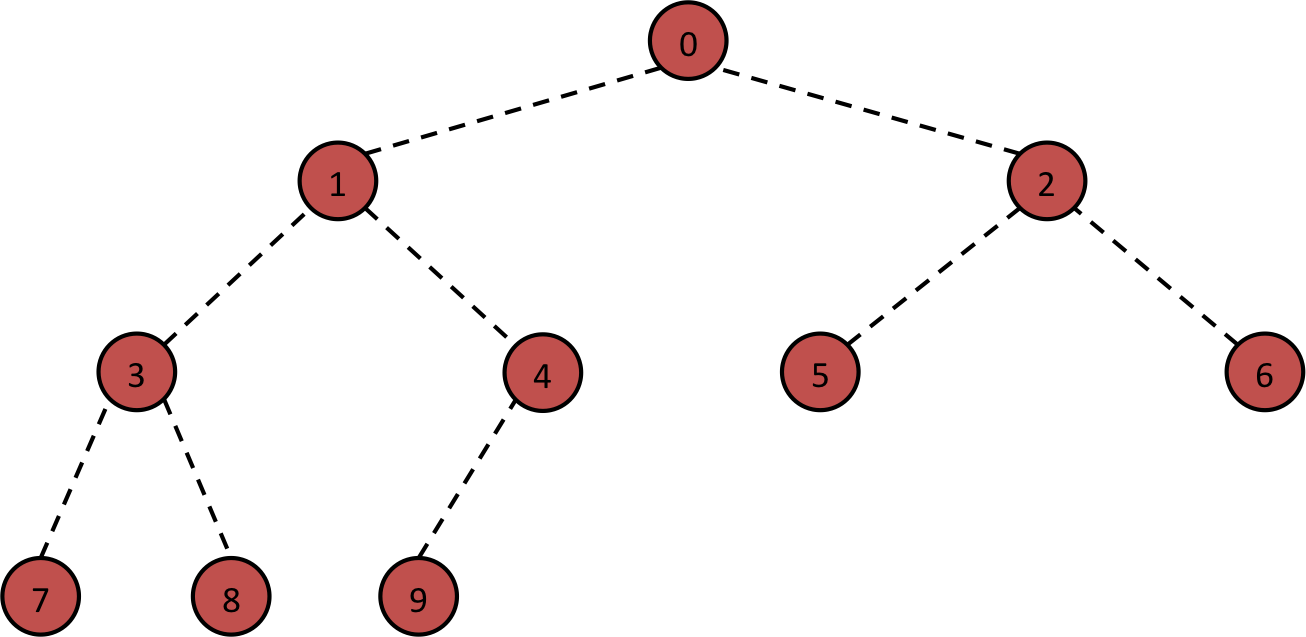
\includegraphics[scale=0.25, clip]{images/heapSort13.png}}\\
	\caption[Heap Sort. Iterations]{Iterations of heap sort}
	\label{fig:heapsort3}
\end{figure}

Because we are using a binary tree, the time complexity of moving an element to the correct position in the heap is $O(\log n)$, and because we need to do it for all $n$ elements in the array, the time complexity of the \textit{Heap Sort} is $O(n \log n)$. The code in \ref{lst:heap_sort} receives an array $X$ of $n$ elements, where $(1 \leq n \leq 100)$ and print the same array $X$, but with its elements sorted in ascending order.\\ 

\noindent \textbf{Time Complexity:} $O(n\log n)$\\
\textbf{Input:}\\
\indent n: The number of elements in the array.\\
\indent X: Array to be sorted.\\
\textbf{Output}:\\
\indent The array sorted.

\begin{lstlisting}[caption={Heap Sort}, label={lst:heap_sort}, numbers=left]
#include <stdio.h>
#define N 101

int X[N];
int n;

void Heap_Sort();
void Make_Heap();
void Down_Heap(int);
void Swap(int, int);

int main()
{
    int i, temp;
    scanf("%d", &n);
    for(i=0; i<n; i++)
        scanf("%d", &X[i]);
    
    temp = n;
    Heap_Sort();

    n = temp;
    for(i=0; i<n; i++)
        printf("%d ", X[i]);

    printf("\n");
    return 0;
}
\end{lstlisting}

The \texttt{Heap\_Sort} function, first converts the array $X$ into a heap by calling the function \texttt{Make\_Heap}, then as explained before, the last element and the first element are swapped, that will cause that the last element to be in the correct position. The heap has to built again, but leaving aside the last element. The process is repeated until the array is completely sorted.

\begin{lstlisting}[numbers=left]
void Heap_Sort()
{
    Make_Heap();
    while(n > 1)
    {
        n--;
        Swap(0,n);
        Down_Heap(0);
    }
}
\end{lstlisting}

Given an array $X$ the \texttt{Make\_Heap} function converts $X$ into a heap. See the example in figure \ref{table:heap_array}.

\begin{lstlisting}[numbers=left]
void Make_Heap()

    int i;
    for(i=n/2-1; i>=0; i--)
        Down_Heap(i);
}
\end{lstlisting}

The function \texttt{Down\_Heap} is essential for the correct operation of the program, it receives an integer $k$, and place the element $X_k$ in the correct position of the heap by doing the necessary swap operations described in \ref{fig:heapsort1}. 

\begin{lstlisting}[numbers=left]
void Down_Heap(int k)
{
    int w = 2*k + 1;
    while(w < n)
    {
        if(w+1 < n)
            if(X[w+1] > X[w])
                w++;

        if(X[k] >= X[w])
            return;

        Swap(k,w);
        k = w;
        w = 2*k + 1;
    }
}
\end{lstlisting}

The \texttt{Swap} function receives two integers $a$, and $b$ and swap the elements $X_a$ and $X_b$ in the array.

\begin{lstlisting}
void Swap(int a, int b)
{
    int temp = X[a];
    X[a] = X[b];
    X[b] = temp;
}
\end{lstlisting}

\section{Sorting with the algorithm library}
Now that we know some of the most popular algorithms to sort, we will see how to make our life easier when we have to sort a set of comparable elements.\\

Most programming languages have a library that help us sort. In \texttt{C++} there is a library called \texttt{algorithm} \index{algorithm library} that contains a method to sort that guarantees a complexity time of $O(nlogn)$. The interesting thing here is that this library allows us to customize our own sorting rules.\\

In order to use the algorithm library we only have to add it and use the \texttt{sort} method. Let's see some code examples. Take a look to the comments inside the code.

\begin{lstlisting}[caption={Simplest sort function}, label={lst:sortFunction_2}, numbers=left]
//This example shows the simplest form to use sort function
#include <stdio.h>
//We include algorithm library
#include <algorithm>
#define N 10
using namespace std;
//Function to print the array elements
void print(int *A, int length){
    for (int i=0; i<length; i++){
        printf("%d ",A[i]);
    }
}

int main()
{
    int arr[N] = {3,5,7,8,2,1,0,9,10,11};
    printf("Unordered array:\n");
    print(arr,N);
    /* sort function uses two parameters, they are the initial
       and final position of the elements that will be sorted */
    sort(arr,arr+N);
    printf("\n");
    printf("Sorted array:\n");
    print(arr,N);
    return 0;
}
\end{lstlisting}
\subsection{Overloading operator <}
So far we have only ordered numbers in a non-decreasing way and based on one parameter, because it is the natural manner, but what if we want to sort in a non-increasing way or taking two parameters into account, to do that we can modify the behavior of the \texttt{sort} function by overloading the operator \texttt{<}. Let's review how to implement it with the following two examples.\\

The first example in \ref{lst:sortFunction_1} sort an array in non-increasing order by overloading the \texttt{<} operator.

\begin{lstlisting}[caption={Sorting in a non-increasing way}, label={lst:sortFunction_1}, numbers=left]
//This example shows how to sort an array in a non-increasing way
#include <stdio.h>
//We include algorithm library
#include <algorithm>
#define N 10
using namespace std;
/* We need a structure to overload
   the operator <, otherwise we
   cannot make it */
struct _int{
    int x;
};
//Function to print the array elements
void print(_int *A, int length){
    for (int i=0; i<length; i++){
        printf("%d ",A[i].x);
    }
}
/* Here we are overloading < operator.
   What we are doing is simply converting
   < operator to > operator.
   In this way we can sort the elements
   in non-increasing form.*/
bool operator <(_int A, _int B){
    return (A.x>B.x);
}

int main()
{
    _int arr[N] = {2,5,7,7,2,1,0,9,10,11};
    printf("Unordered array:\n");
    print(arr,N);
    /* sort function uses two parameters, they are the initial
       and final position of the elements that will be sorted */
    sort(arr,arr+N);
    printf("\n");
    printf("Sorted array in non-increasing way:\n");
    print(arr,N);
    return 0;
}
\end{lstlisting}

In the second example in \ref{lst:sortFunction_2} we sort an array of points, first in increasing order according to their x-coordinate, and if two points have the same x-coordinate, then they are sorted in increasing order by their y-coordinate.

\begin{lstlisting}[caption={Sorting pairs in non-increasing form}, label={lst:sortFunction_2}, numbers=left]
//This example shows how to sort a list of pairs in non-decreasing way
#include <stdio.h>
//We include algorithm library
#include <algorithm>
#define N 10
using namespace std;
/* We need a structure _pair
   to overload the operator < */
struct _pair{
    int x,y;
};
//Function to print the pairs
void print(_pair *A, int length){
    for (int i=0; i<length; i++){
        printf("%d %d\n",A[i].x,A[i].y);
    }
}
/* As the x parameter is the first criteria to sort,
   we check first the 'x' member, then if A and B have
   the same 'x' we compare 'y' parameter, making 'y'
   second sorting criteria. */
bool operator <(_pair A, _pair B){
    return (A.x<B.x || (A.x==B.x && A.y<B.y));
}

int main()
{
    //Pair list
    _pair arr[N] = {{2,3},{5,7},{5,2},{1,0},{1,-1},{-2,2},{-2,0},{-2,0},{0,0},{0,1}};
    printf("Unordered array of pairs:\n");
    print(arr,N);
    /* sort function uses two parameters, they are the initial
       and final position of the elements that will be sorted */
    sort(arr,arr+N);
    printf("\n");
    printf("Pairs sorted by x parameter as first criteria and y\n"
           "parameter as second one in non-decreasing form:\n");
    print(arr,N);
    return 0;
}
\end{lstlisting}
\subsection{Adding a function to sort}
Sometimes it is better to add a function instead of overloading an operator, this is used when you need to sort a complex structure or in a special way. For example suppose we have to sort characters, digits [0-9] and letters [a-z][A-Z], such that the letters have greater priority than numbers. To do that we need to implement a function that allows us to alter the ASCII natural order, in which the numbers are first than the letters. Let's look at the code to see how it works.
\begin{lstlisting}[caption={Sorting the letters first than the digits}, label={lst:sortFunction_1}, numbers=left]
//This example shows how to implement a custom function to sort
#include <stdio.h>
#include <algorithm>
#define N 10
using namespace std;
//Function to print the array elements
void print(char *A, int length){
    for (int i=0; i<length; i++){
        printf("%c ",A[i]);
    }
}
bool sort_first_letters(char A, char B){
    //case where A is digit
    if (A>='0' && A<='9'){
        //sub-case where B is also digit
        if (B>='0' && B<='9'){
            //we return based on the ASCII natural order
            return (A<B);
        }
        //sub-case where B is letter
        else{
            /* Since A is digit and B is letter
               it returns false because we want
               first the letters */
            return false;
        }
    }
    //case where A is letter and B is digit
    if (B>='0' && B<='9'){
        /* Since A is letter it returns
           true because we want first the
           letters */
        return true;
    }
    //case where A and B are letters, here we return the ASCII natural order
    return (A<B);
}
int main()
{
    //Character array
    char arr[]={'7','5','3','1','a','n','z','A','N','Z'};
    printf("Array as defined: \n");
    print(arr,N);
    printf("\n");
    //Here we use the normal sort
    sort(arr,arr+N);
    printf("Sorted array according to ASCII table: \n");
    print(arr,N);
    printf("\n");
    //Here we use custom function in order to sort by our criteria
    sort(arr,arr+N,sort_first_letters);
    printf("Sorted array according to letters first than digits criteria: \n");
    print(arr,N);
    return 0;
}

\end{lstlisting}
\section{Problems}

In this section we present special cases of sorting problems that can be solved using techniques different form the ones mentioned previously in this chapter. This with the objective that the reader be aware that there can be other approaches when facing problems that involves sorting. Solutions that sometimes are easier to implement and have better performance. Said that, we encourage the reader to try to solve the problems first, before reading the solution. 

\subsection{Marching in the school}

$N$ students are standing in one line, some of them are facing left, and other facing right. All of them must face to the same direction, so when a student see the face of another student understands that he has made a mistake and turns around. The process continues until all the students don't see any other student's face. Write a program that calculates the number of times when a pair of students turned around. If the process is infinite, print "NO".

\begin{table}[H]
\caption{Marching in the school}
\centering % used for centering table
\begin{tabular}{|c|l|c|}
\hline %inserts double horizontal lines
\textbf{Formation} & \textbf{Comments} & \textbf{Number of turns} \\
\hline % inserts single horizontal line
$>><<><$ & Initial formation & 2 \\
$><><<>$ & One second has passed & 2 \\
$<><><>$ & Two seconds has passed & 2 \\
$<<><>>$ & Three seconds has passed & 1 \\
$<<<>>>$ & Final formation & 0 \\
\hline
\multicolumn{2}{|c|}{} & Total: 7 \\
\hline %inserts single line
\end{tabular}
\end{table}

\subsection*{Input}

The first line of the input contains the number of students $N$ $(1 \leq N \leq 30000)$. The rest of the input contains only $"<"$, $">"$ characters. There is exactly $N$ $"<"$ and $">"$ characters in the input file.

\subsection*{Output}

Write the number of turns.

\begin{table}[H]
\centering % used for centering table
\begin{tabular}{|l|l|}
\hline %inserts double horizontal lines
\textbf{Sample Input} & \textbf{Sample Output} \\
\hline % inserts single horizontal line
6 & 7\\ 
$>><<><$ & \\
\hline %inserts single line
\end{tabular}
\end{table}

\subsection*{Solution}

The solution for this problem consists on identifying when a $<$ character appears, and when that happens increase the result by the number of $>$ characters before it.

\begin{lstlisting}[caption={Marching in the School}, label={lst:marching_school}, numbers=left]
#include <stdio.h>

int main()
{
    long n, k, r, sum;
    int c;
    
    scanf("%ld", &n);

    k = 0;
    r = 0;
    sum = 0;

    while(k < n)
    {
        c = getc(stdin);
        if(c == '>' || c == '<')
            k++;
        if(c == '>')
            r++;
        else if(c == '<')
            sum += r;
    }

    printf("%ld\n", sum);
    
    return 0;
}
\end{lstlisting}

\subsection{How Many Swaps?}

Given an  array $X$ of $n$ elements write a program that determines the number of swaps needed to sort the array $X$ using \textit{Bubble Sort}.

\subsection*{Input}

The first line of the input contains $n$ $(1 \leq n \leq 100)$, indicating the number of elements in the array $X$. The next $n$ numbers represent the elements of $X$, all of them 32-bit integers.

\subsection*{Output}

The number of swaps made by the \textit{Bubble Sort} method.

\subsection*{Solution}

One option is to implement the \textit{Bubble Sort} algorithm and count the number of swaps that occur. Another option is to count the number of misplaced elements in the array. The later option consists on counting for each element in the array, the number of elements at its right that are smaller. Consider the following array

$$
X = [3,7,2,6,1,4,3,5]
$$

If we look at the elements at the right of the first element (3), we notice that there are two elements that are smaller (1 and 2). So we increase our counter by two. We do the same for the second element (7), this time we have six elements smaller than it, so we increase our result by six. If we follow the same process for all elements we obtain that our answer is:

$$
2 + 6 + 1 + 4 + 0 + 1 + 0 + 0 = 14
$$

\begin{lstlisting}[caption={How Many Swaps}, label={lst:how_many_swaps}, numbers=left]
#include <cstdio>
#define N 100

using namespace std;

int main()
{
    int i, j, n, ans;
    int X[N];
    
    scanf("%d", &n);
    for(i=0; i<n; i++)
        scanf("%d", &X[i]);
		
    ans = 0;
    for(i=0; i<n; i++)
    {
        for(j=i+1; j<n; j++)
        {
            if(X[i] > X[j])
            ans++;
        }
    }
	
    printf("%d\n", ans);
    
    return 0;
}
\end{lstlisting}


\section{Chapter Notes}

Fastest sorting methods run in $O(n \log n)$ time, but they are sometimes a little bit harder to implement. On the other hand, algorithms that run in $O(n^2)$ time tend to be easier to implement, but their performance is poor when dealing with a large amount of data. When the number of elements to sort is greater than $1000$, we recommend not to use a $O(n^2)$ algorithm. In fact is a good practice to use the \texttt{sort} function of the \texttt{algorithm}  \index{algorithm library} library whenever is possible.\\
 
Is important to keep in mind those methods that are not based on comparisons, like the Counting Sort. They are faster for some situations and are easy to implement.\\ 

The book of \textit{Introduction to Algorithms} \cite{cormen} contains a deeper explanation and analysis of the Heap Sort and Quick Sort algorithms, and provides a great review of some techniques used to sort in linear time like the Counting Sort. Sedgewick \cite{sedgewick} makes an analysis of different sorting methods, mentioning their advantages and disadvantages, and include code for most of them written in C/C++. Knuth \cite{knuth3} describes with great detail the performance of different sorting algorithms, always providing  a mathematical perspective.\\

A brief explanation of sorting algorithms can be found in topcoder tutorials \cite{sorting-topcoder}. And some problems involving sorting and searching can be found in the following online judges:

\begin{itemize}
    \item \url{https://uva.onlinejudge.org/index.php?option=com_onlinejudge&Itemid=8&category=98}
    \item \url{http://acm.timus.ru/problemset.aspx?space=1&tag=beginners}
\end{itemize}

\newpage
\section{Exercises}

\begin{tcolorbox}
\begin{enumerate}
    \item Write a program that reads a number $n$ $(2 \leq n \leq 10^6)$ followed by $n$ pair of numbers representing $(x,y)$ coordinates, and print those coordinates sorted in increasing order according to their x-coordinate, and if there is a tie then sort them in increasing order according to their y-coordinate. Assume that all coordinates are integers in the range $[-10^5,10^5]$.
    \item Certain country is divided into regions, and each region has determined number of citizens. They are about to choose their leader, and the only condition for a person to be the leader is that he or she must obtain control of the majority of the regions. A person gain control of a region if the majority of the citizens of that region vote for that person. Write a program that given the number of regions and the numbers of citizens in each region, find the minimum number of votes a person needs to become the leader. The number of regions is no more than $100000$.
    \item The conclave is the ritual where all cardinals of the Catholic church choose the new pope. The pope is elected among the cardinals and all of them vote for the one they want to be the new pope. The pope is the one that gets at least $2/3$ of the votes. For simplicity suppose that the cardinals are numbered from $1$ to $n$. Write a program that reads an integer $n$ $(1 \leq n \leq 1000)$ indicating the number of cardinals, followed by $n$ numbers representing the votes of each cardinal. The output is the number associated to the new pope.
\end{enumerate}
\end{tcolorbox}

\chapter{Data Structures}
\begin{chapquote}{Author's name, \textit{Source of this quote}}
"This is a quote and I don't know who said this."
\end{chapquote}

Data structures is a fundamental part of computer programming, since they are used to store our data. An array, a matrix, or any multi-dimensional array are examples of a data structure.\\

During this chapter we will review some of the most used data structures, we will analyze their properties and use cases, because depending of the circumstances some are more apt than others.\\

Lets analyze a simple array and possible uses cases. Suppose we have an array $X$ of $n$ elements, $X_0, X_1, \ldots, X_{n-1}$. Now, what if we want to extract the $10^{th}$ element of the array? Well, that is easy, we just go and retrieve the element $X_{10}$. That simple operation of retrieving certain element runs in $O(1)$ time. Now, suppose we want to find certain element in $X$, well, in that case we must go trough the whole array and check element by element until we find the one we are looking for. That task run in $O(n)$ time. Finally consider the case of removing one element from $X$. That is not a simple task, since we must remove the desired element and shift all the elements at its right. That task has a $O(n)$ running time.\\

The time complexity for insertion, extraction, finding, and deletion operations varies depending on the data structure used. Some are fast to extract information like vector or arrays, other are faster to insert or remove data like lists, other like trees are more suitable to find elements. This will be the purpose of this chapter, to analyze the pros and cons of each data structure and how they work.

\newpage
\section{Linear Data Structures}

In this section we will review the basic data structures. Let's start saying what is a data structure. A data structure is basically one tool for storage data in memory with a specific purpose when you are coding, besides inherently associated with the data structure are the operations over it. This operations are normally insert, delete and find one element or a set of elements inside it.\\ 

For the code in this section we are going to separate the Memory Complexity in general and the Time Complexity for each of operations over the data structure. 

\subsection{Stack}
This data structure is used under principle \textit{last in first out}, that means the last element inserted will be the first element removed. A real life case to exemplify how a stack works is how to dry a stack of washed dishe. We stack the dishes as we wash them, so the last plate washed will be the first to be dried, and so on until we have no plates anymore. Stacks are very useful in Computer Science in general, they are the basis of the recursion and they are utilized in Depth First Search indirectly when the recursion is applied, as we will se in chapter \ref{chap:graphs}. In programming contests is common to use stacks when you are solving problems related with evaluate mathematical expressions and parenthesis balance.

\noindent
\newline
\textbf{Memory Complexity:} $O(n)$ \\
\textbf{\textit{Insert} Time Complexity:} $O(1)$ \\
\textbf{\textit{Delete} Time Complexity:} $O(1)$ \\
\textbf{\textit{Find} Time Complexity:} $O(n)$\\ 

\noindent
\textbf{Input:}\\
\indent List of numbers(it can be any abstract data type) that will be stored in the stack.\\
\noindent \textbf{Output}:\\
\indent Depends of the operation, the current state of the stack. The operations performed will be insert, known as push, and delete, known as pop.
\begin{lstlisting}
//Stack simulated with array
#include <iostream>
#include <stdio.h>
using namespace std;
//index l (last) to manage the stack
int s[100],l;
void push(int x){
    s[l++]=x;
}
int pop(){
    int x=s[l--];
    return x;
}
bool isEmpty(){
    return (l==0);
}
void print(){
    for (int i=0; i<l; i++){
        printf("%d ",s[i]);
    }
    printf("\n");
}
int main()
{
    //Insert numbers from 1 to 5
    printf("First stack state after insert [1-5]:\n");
    for (int i=1; i<=5; i++){
        push(i);
    }
    //See the state of the stack
    print();
    //Delete the last 2 elements inserted
    pop();
    pop();
    printf("Stack state after 2 deletes:\n");
    //See the state of the stack
    print();
    //Insert one element
    push(4);
    printf("Stack state after 1 insert (number 4):\n");
    //See the state of the  stack
    print();
    //Clear the stack
    while (!isEmpty()){
        pop();
    }
    printf("Stack empty\n");
    return 0;
}


\end{lstlisting}
A stack also can be simulated with a linked list, but the concept is the same. In section \ref{sec:stl} we are going to see how to use a stack from the \textit{Standard Template Library (STL)}.
\subsection{Queue}
This data structure is used under principle of \textit{first in first out}, that means that the first element inserted will be the first element removed. A real life case to illustrate how a queue works is the line formed in a market to pay, the first person to arrive is the first person to be served.  Queue is as common as stack in Computer Science. Inside a contest is required to implement the \textit{Breadth First Search}, as we will see in chapter \ref{chap:graphs}, and is useful to solve problems where they ask us the state of certain list that is modified over time.

\noindent
\newline
\textbf{Memory Complexity:} $O(n)$ \\
\textbf{\textit{Insert} Time Complexity:} $O(1)$ \\
\textbf{\textit{Delete} Time Complexity:} $O(1)$ \\
\textbf{\textit{Search} Time Complexity:} $O(n)$\\ 

\noindent
\textbf{Input:}\\
\indent List of numbers(it can be any abstract data type) that will be stored in the queue.\\
\textbf{Output}:\\
\indent Depends of the operation, the current state of the queue. The operations performed will be insert, known as push, and delete, known as pop.
\begin{lstlisting}
//Queue simulated with array
#include <iostream>
#include <stdio.h>
using namespace std;
//index f(front) and b(back) to manage the queue
int q[100],f,b;
void push(int x){
    q[f++]=x;
}
int pop(){
    int x=q[b++];
    return x;
}
bool isEmpty(){
    return (b==f);
}
void print(){
    for (int i=b; i<f; i++){
        printf("%d ",q[i]);
    }
    printf("\n");
}
int main()
{
    //Insert numbers from 1 to 5
    printf("First queue state after insert [1-5]:\n");
    for (int i=1; i<=5; i++){
        push(i);
    }
    //See the state of the queue
    print();
    //Delete the first elements inserted
    pop();
    pop();
    printf("Queue state after 2 deletes:\n");
    //See the state of the queue
    print();
    //Insert one element
    push(4);
    printf("Queue state after 1 insert (number 4):\n");
    //See the state of the  stack
    print();
    //Clear the stack
    while (!isEmpty()){
        pop();
    }
    printf("Queue empty\n");
    return 0;
}
\end{lstlisting}
As a stack, a queue also can be simulated with a linked list and there is no any change conceptually. The STL library has a queue implemented too, and we will see it in section \ref{sec:stl}.

\subsection{Linked List}
It is not common to use this data structure inside a programming contest, but it's very useful in Computer Science. A linked list can be thought as an array, but the difference is that it allow us to insert and delete in constant time increasing  or decreasing the size of the structure.\\

There are various types of linked list, some of them are: simple linked list, double linked list, circular linked list, double circular linked list, among others.\\

A linked list is composed by nodes, these nodes store  data, like the arrays, but they also save the memory address of some node related to this node. The relationship between nodes can be next node, previous node, child node, parent node, sibling node or what the programmer wants to think in his/her mind.\\

In a linked list is necessary to know where is the beginning and the end of the list, known as head and tail of the list. Normally the tail node points to \texttt{NULL}.\\

In simple linked list, doubly linked list, circular linked list and doubly circular linked list the operation has the same time and memory complexity.

\noindent
\newline
\textbf{Memory Complexity:} $O(n)$ \\
\textbf{\textit{Insert} Time Complexity:} $O(1)$ \\
\textbf{\textit{Delete} Time Complexity:} $O(1)$ \\
\textbf{\textit{Search} Time Complexity:} $O(n)$

\subsubsection{Simple Linked List}
\index{simple linked list}
A \textit{simple linked list} is a linked list where a node stores only the information about the next node address, and the main information of the node. The last node points to \texttt{NULL}. The source code in \ref{lst:simple_linked_list} define the class \texttt{Node}, which contains an integer value to store the information associated to that node, and a pointer to the next node in the list. The node \texttt{head} points to the first node of the list, and the node \texttt{tail} points to the last node of the list. The \texttt{main} function add elements into the list and then remove them from the list.
 
\noindent
\newline
\textbf{Input:}\\
\indent List of numbers (it can be any data abstract type) that will be stored in the simple linked list.\\
\textbf{Output}:\\
\indent Depends of the operation, the current state of the simple linked list. The operations performed will be insert, delete and search.
\begin{lstlisting}[caption={Simple Linked List}, label={lst:simple_linked_list}, numbers=left]
#include <cstdio>

using namespace std;

class Node
{
    public:
    
    int val;
    Node *next;
    
    Node(int val, Node *nextNode)
    {
        this->val = val;
        this->next = nextNode;
    }
};

Node *head = NULL;
Node *tail = NULL;

void pushBack(int);
void popFront();
void printList();

int main()
{
    //Insert three elements in the list
    pushBack(2);
    pushBack(3);
    pushBack(5);
    printList();
    
    //Remove the first element
    popFront();
    printList();
    
    //Remove the other two elements
    popFront();
    popFront();
    printList();
    
    return 0;
}
\end{lstlisting}

The \texttt{pushBack} function add a node at the end of the list. The new node becomes the tail, and the \texttt{next} pointer of the node that was previously the tail is modified and points to the new node.  

\begin{lstlisting}
void pushBack(int val)
{
    Node *newNode = new Node(val,NULL);
    
    if(tail == NULL)
        head = newNode;
    else
        tail->next = newNode;
    
    tail = newNode;
}
\end{lstlisting}

The \texttt{popFront} function removes  the first element of the list, if there is any. The node associated to the \texttt{next} pointer of the head becomes the head, and the node that was previously the head is removed.

\begin{lstlisting}
void popFront()
{
    if(head != NULL)
    {
        Node *nextNode = head->next;
        
        delete(head);
        
        head = nextNode;
        if(head == NULL)
            tail = NULL;
    }
}
\end{lstlisting}

The function \texttt{printList} as its name says print the whole list by iterating trough all its elements printing them one by one. If the list is empty prints the message \textit{''-- empty list --''}.

\begin{lstlisting}
void printList()
{
    Node *curNode = head;
    
    if(curNode == NULL)
    {
        printf("-- empty list --\n");
        return;
    }
    
    while(curNode != NULL)
    {
        printf("%d", curNode->val);
        curNode = curNode->next;
        
        if(curNode != NULL)
            printf(" -> ");
    }
    
    printf("\n");
}
\end{lstlisting}
\subsubsection{Doubly Linked List}
\index{doubly linked list}
A doubly linked list is a linked list where a node stores the memory address  about the next node and the previous one. The link to the next node of the last node  points to \texttt{NULL}, and the link to the previous node of the first node points to \texttt{NULL} as well. The program in \ref{lst:doubly_linked_list} defines a class \texttt{Node} similar to the one used in the \textit{Simple Linked List}, but it adds a pointer to the previous node. The functions \texttt{pushBack} and \texttt{popFront} are similar to the ones in the \textit{Simple Linked List} implementation, but include some changes that modify the \texttt{next} and \texttt{prev} links of the nodes involved in the insertion or deletion process. 

\noindent
\newline
\textbf{Input:}\\
\indent List of numbers(it can be anything) that will be stored in the doubly linked list.\\
\textbf{Output}:\\
\indent Depends of the operation, the current state of the doubly linked list. The operations performed will be insert, delete and search.
\begin{lstlisting}[caption={Doubly Linked List}, label={lst:doubly_linked_list}, numbers=left]
#include <cstdio>

using namespace std;

class Node
{
    public:
    
    int val;
    Node *next;
    Node *prev;
    
    Node(int val, Node *nextNode, Node *prevNode)
    {
        this->val = val;
        this->next = nextNode;
        this->prev = prevNode;
    }
};

Node *head = NULL;
Node *tail = NULL;

void pushBack(int);
void pushFront(int);
void popFront();
void popBack();
void printList();

int main()
{
    //Add two elements at the end of the list
    pushBack(5);
    pushBack(7);
    printList();
    
    //Removes the last element
    popBack();
    printList();
    
    //Removes the last element and the list is empty
    popBack();
    printList();
    
    //Add five elements at the top of the list
    pushFront(6);
    pushFront(8);
    pushFront(3);
    pushFront(1);
    pushFront(4);
    printList();
    
    /Removes the last element and the two first elements
    popBack();
    popFront();
    popFront();
    printList();
    
    return 0;
}
\end{lstlisting}

Let be $p$ the current tail. When we add an element to the back of the list, the new node becomes the tail with its \texttt{prev} link pointing to $p$, and the \texttt{next} link of $p$ pointing to the new tail.

\begin{lstlisting}
void pushBack(int val)
{
    Node *newNode = new Node(val,NULL,NULL);
    
    if(tail == NULL)
    {
        head = newNode;
    }
    else
    {
        newNode->prev = tail;
        tail->next = newNode;
    }
    
    tail = newNode;
}
\end{lstlisting}

The \texttt{pushFront} function inserts an element at the beginning of the list. The new node becomes the head with its \texttt{next} link pointing to the node that was previously the head.

\begin{lstlisting}
void pushFront(int val)
{
    Node *newNode = new Node(val,NULL,NULL);
    
    if(head == NULL)
    {
        tail = newNode;
    }
    else
    {
        newNode->next = head;
        head->prev = newNode;
    }
    
    head = newNode;
}
\end{lstlisting}

The \texttt{popFront} function removes the first element of the list. The node associated to the \texttt{next} link of the head becomes the new head, and the previous head is removed from the list.

\begin{lstlisting}
void popFront()
{
    if(head != NULL)
    {
        Node *nextNode = head->next;
        
        if(nextNode != NULL)
            nextNode->prev = NULL;
        
        delete(head);
        
        head = nextNode;
        if(head == NULL)
            tail = NULL;
    }
}
\end{lstlisting}

Similar to the \texttt{popFront} function, the \texttt{popBack} function removes the last element of the list. The tail is removed and node associated to its \texttt{prev} link becomes the new tail.

\begin{lstlisting}
void popBack()
{
    if(tail != NULL)
    {
        Node *prevNode = tail->prev;
        
        if(prevNode != NULL)
            prevNode->next = NULL;
        
        delete(tail);
        
        tail = prevNode;
        if(tail == NULL)
            head = NULL;
    }
}
\end{lstlisting}

\subsubsection{Circular Linked List}
\index{circular linked list}

A circular linked list is almost exactly the same as a simple linked list, but there is a light difference, and is that instead of having the last node pointing to \texttt{NULL}, it points to the first node, and hence the name. The code for the \textit{Circular Linked List} is almost the same that the one in \ref{lst:simple_linked_list}, with just one difference, every time that the list is modified, because of an insertion or a deletion, we have to make sure that the tail is linked to the head. Basically we must add the following statement.

\begin{lstlisting}[frame=none]
if(tail != NULL)
    tail->next = head;
\end{lstlisting}

\subsubsection{Doubly circular Linked List}
\index{doubly circular linked list}
A doubly circular linked list is practically the same as a doubly linked list, but with  a tiny  difference, the last node has a link to the first node, and conversely the first node has a link that points to the last one. The implementation is very similar to the program \ref{lst:doubly_linked_list}, but again we must be careful when the list is modified by an insertion or a deletion by ensuring that the first and last element of the list are linked in both ways. We can do that by adding the following sentences:

\begin{lstlisting}[frame=none]
if(head != NULL)
{
    head->prev = tail;
    tail->next = head;
}
\end{lstlisting}

\section{Trees}
So far we have reviewed linear data structures, but there is more, in this section we will discuss tree-shaped data structures. Let's start by defining a tree from the graph theory perspective. A tree is a simple graph (graph without multiple edges) with no cycles. This definition may be not too useful to picture a tree as a data structure. Perhaps it is better to think about it as a multilevel structure to store information.\\

Before continuing it is necessary to understand the following terminology:\\

\noindent
\textbf{Root: } Top node of the tree.
\newline
\textbf{Child: } Node pointed by other node in a previous level.
\newline
\textbf{Parent: }Node that points to a node at the next level.
\newline
\textbf{Siblings: }Nodes that comes from same parent.
\newline
\textbf{Leaf: }Node with no children.
\newline
\textbf{Ancestor: }Node that is before another node coming from root.
\newline
\textbf{Descendant: }Node that is after another node coming from root.
\newline
\textbf{Path: }Sequence of nodes connected.
\newline

Trees are present in different areas, one of the main applications is in the file systems, when we create a file or a folder somewhere internally we are creating a child from a specific node, which represents the folder. Other applications are related with keep elements ordered and apply queries over it, one example of this is an index in some \texttt{SQL} package.

\subsection{Tree Traversal}

\subsection{Binary Search Tree}

\subsection{AVL Tree}

\subsection{Segment Tree}

\section{Binary Indexed Tree (BIT)}

\index{BIT} 
Suppose we have an array composed by numbers $a_0,a_2,...,a_{n-1}$ and we want to know what is the sum from the index $i$ to index $j$, $0 \leq i \leq j < n$ . The naive approach is go through the interval and sum element by element. If this query is performed once the time cost is $O(n)$, but if we have $m$ queries of this type, the complexity time tends to $O(mn)$. This complexity can be reduced by saving the accumulate sums using another array to store the accumulate from the index $0$ to the index $i$, this might be done in linear time, then to resolve the query sum\{$a_i, a_j$\}, we just calculate the difference between the accumulate of the index $j$ and the accumulate of the index $i-1$. This last operation is made in constant time $O(1)$. So far everything seems good enough, but the last algorithm is considering an static array, in other words, the array is never modified, but what if we want to update the array and make queries at the same time. Here is when BIT shows up, BIT allows us to solve the problem of the sum of an interval when this is not static.\\

The idea behind BIT consists on storing the accumulates from index $0$ to index $i$ using a binary representation of the indexes. A BIT is also known as a Fenwick tree, since it was proposed by Peter Fenwick in 1994 \cite{fenwick}.\\

Before to proceed with the explanation, let's see a bitwise trick. The trick consists on isolating the last non-zero bit of a number (keep the last non-zero bit and put 0's in the other bits) by using the fact that computer represent a negative number as two's complement. See image \ref{fig:bit1}

\begin{figure}[H]
	\centering
	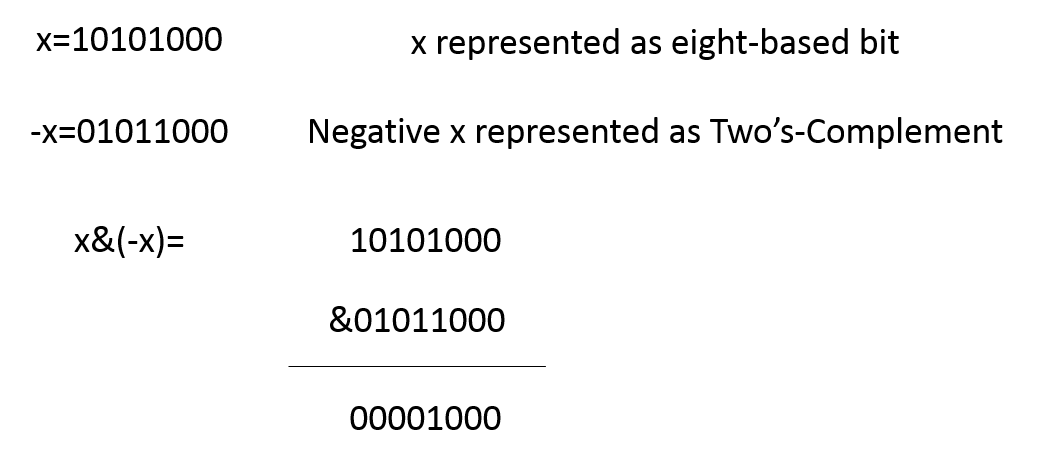
\includegraphics[scale = 0.6]{images/BIT_1.png}
	\caption[Bitwise operation to get rightmost bit]{Bitwise operation to get the less significant bit}
	\label{fig:bit1}
\end{figure}

Be $C_i$ the accumulate sum from index $0$ to some index $i$, and be $T$ the array that represents the BIT. Is important to mention that indexes of $T$ starts from $1$ and not from $0$, meaning that $T$ is an array with indexes from $1$ to $n$. For example, suppose we want to obtain the value of $C_{10}$, using the array $T$ this is accomplished with the following sum:

$$
C_{10} = T_{1011} + T_{1010} + T_{1000}
$$

The first thing to do is add 1 to the given index, since the indexes in $T$ starts from $1$. Then we do a binary representation of that number, in this case 11, which is 1011, an then, using the bitwise trick explained before, we convert the last 1 from that number into a 0 to obtain the new index. We continue doing this until the index is zero.

$$
1011 \rightarrow 1010 \rightarrow 1000 \rightarrow 0000
$$

The code in \ref{lst:bit} shows a basic implementation of a BIT. It contains three functions. The function \texttt{updateBIT} add a value of $v$ to node $i+1$ and to all its ancestors. The function \texttt{queryBIT} receives an integer $i$ and returns the accumulate sum of all numbers in the original array from index $0$ to index $i$. And the function \texttt{createBIT}, which creates the BIT from the original array.\\

The time complexity of the \texttt{queryBIT} and the \texttt{updateBIT} functions is $O(\log n)$ for both. On the other hand, the tume complexity of the \texttt{createBIT} is $O(n \log n)$, since we have to update the BIT for each element in the array.\\

\noindent \textbf{Time Complexity:}\\
\indent \textit{creation:} $O(n\log n)$\\
\indent \textit{query:} $O(\log n)$\\
\indent \textit{update:} $O(\log n)$\\
\textbf{Input:}\\
\indent N: The number of elements in the array.\\
\indent X: Array with integer numbers.\\
\textbf{Output}:\\
\indent Queries using a BIT to obtain the sum $X[0] + \cdots + X[i]$, for some $i$.

\begin{lstlisting}[caption={BIT}, label={lst:bit}, numbers=left]
#include <cstdio>
#define N 10

using namespace std;

int X[N] = {1,4,2,4,3,0,7,5,1,6}; 
int T[N+1];

void updateBIT(int, int);
int queryBIT(int);
void createBIT();

int main()
{
    createBIT();
    
    //Print the accumulate sum from X[0] to X[6]
    printf("%d\n", queryBIT(6));
    
    //Print the accumulate sum from X[0] to X[9]
    printf("%d\n", queryBIT(9));
    
    //Add 2 to X[5] and print the sum from X[0] to X[9]
    updateBIT(5,2);
    printf("%d\n", queryBIT(9));
    
    return 0;
}

void updateBIT(int i, int v) 
{
    i++;
    
    while(i<=N) 
    {
        T[i] += v; 
        i += (i&-i);
    }
}

int queryBIT(int i) 
{
    int res = 0; 
    
    i++;
    
    while(i>0) 
    {
        res += T[i]; 
        i -= (i&-i);
    } 
    
    return res;
}

void createBIT()
{
    int i;
    
    for(i=0; i<N; i++)
        updateBIT(i, X[i]);
}
\end{lstlisting}


\section{Standard Template Library (STL) C++}
\label{sec:stl}
STL is one of the most powerful thing C++ language has. Inside this library are implemented many algorithms and data structures that are very handy for the programming contests. Let's take a look at some of the most common data structures and their respective examples.
\subsection{Unordered Set}
This structure allows us to create an unordered set of unique elements, that means no matter the order just the unicity of the elements. Internally this structure is implemented as a hash table, which is a table that associates keys with values in constant time $O(1)$. It's important to say that this structure is available from the standard  c++11. Imagine we want to count the numbers of different words in some text. We are going to use an unordered set in order to solve the problem. As the set don't let us save repeated elements, it will be sufficient to read the word and store it into the the set and at the end the set will have saved only the different elements, so we can get the size of the set and this will be the answer. Let's look at the code.\\
\newline
\noindent \textbf{Time Complexity:} $O(nl)$\\
\indent l is the length of the longest word. \\
\textbf{Input:}\\
\indent n: Number of word in the text.\\
\indent str: A string representing each word of the text. \\
\textbf{Output}:\\
\indent Number of different words in the text.

\begin{lstlisting}[caption={Number of different words}, label={lst:UnorderedSet_1}, numbers=left]
#include <iostream>
#include <string.h>
#include <unordered_set>
using namespace std;
unordered_set<string> u_set;
int main()
{
    int n;
    string str;
    //We read the number of words we have in our text
    cin>>n;
    //We read the words
    for (int i=0; i<n; i++){
        cin>>str;
        //We insert all the words we read because the repeated words won't be taken into account
        u_set.insert(str);
    }
    cout<<"The number of different words is: "<<endl;
    cout<<u_set.size()<<endl;
    cout<<"The words different are: "<<endl;
    /* There is a new thing in C++ 11 called auto that makes life easier,
       auto substitutes this expression: set<string>::iterator it,
       (*it) means we want the value saved in iterator it, in our case
       the string.
     */
    for (auto it=u_set.begin(); it!=u_set.end(); ++it){
        cout<<(*it)<<endl;
    }
    return 0;
}

\end{lstlisting}

\subsection{Ordered Set}
This structure is almost the same as the unordered set, the only difference is that here the order matters, and actually that can be an advantage in some cases. Internally an ordered set is implemented as a binary search tree, so that guarantees $O(log)$ for the searches, insertions and eliminations. \\

Let's think in the following problem, suppose we have a list of discrete 2D-points and over the list we make operations like deletes, insertions and queries, the insertions will be simple, they give us a 2D point and we have to add it to our list, if the point is already there we ignore it otherwise we add it, then for the eliminations they give us a point and we need to remove it if exists otherwise do nothing. The queries will be more interesting and we will have two types. In first kind of query they give us a point and two discrete distances, that defines a rectangle, the point will be the bottom-left corner and the integers will be the the length (x-coordinate) and width (y-coordinate) of the rectangle and we want to respond the numbers of points that the defined rectangle contains. In the second type they give us a point and we have to answer the minimum difference between the norm of that point and all the norms of the points present in the plane. We define the norm of a point as the distance from the origin. \\

This problem is not trivial and could be an easy-intermediate problem in a ICPC Latin America Regional Contest, so let's start thinking what do we need to solve it. First of all we need a structure to keep the 2D-points list updated and also the structure should allow us perform the queries easy and fast. Thereby an ordered set fits perfectly to solve the problem. To do the insertions and eliminations we only need to use the methods already implemented in a set structure. Then to perform the queries we are going to use the fact that the set saves the elements in a ordered way and also we can use two handy methods that are already implemented in the STL, these methods are lower\_bound and upper\_bound. Let's see how the methods work, both methods returns an iterator, lower\_bound returns an iterator where the value is equal or greater than the element sent in the argument, while upper\_bound returns an iterator where the value is strictly greater than the element sent in the argument. For the first query we can do a double for over the discrete values of the defined rectangle and see if they are in the set. For the second query we have to save the norms in a set, then get the norm of the given point and use lower\_bound or upper\_bound to get the closest distances and obtain the minimum.  \\
\newline
\noindent \textbf{Time Complexity:} $O(n\log n)$\\
\textbf{Input:}\\
\indent n: Number of operations to be performed.\\
\indent operation: Insert, delete or query operation. \\
\textit{Insertion case} \\
\indent x1, y1: Integer coordinates of the point that will be inserted. \\
\textit{Elimination case} \\
\indent x1\, y1: Integer coordinates of the point that will be removed. \\
\textit{Query case} \\
\indent x1, y1, x2, y2: Integer coordinates of the points that defines the rectangle according to the problem. \\
\textbf{Output}:\\
\indent In query case the number of points into the defined rectangle.

\begin{lstlisting}[caption={Number of 2D-points into a given rectangle}, label={lst:OrderedSet_1}, numbers=left]
#include <iostream>
#include <set>
#include <algorithm>
using namespace std;
typedef pair <int,int> point;
//We make a set of points
set <point> s;
int main ()
{
  int x1,y1,x2,y2,ans,n,operation;
  //We read the number of operations we are going to perform
  cin>>n;
  for (int i=0; i<n; i++){
    cin>>operation;
    switch (operation){
        //Insertion case
        case 1:
            cin>>x1>>y1;
            //make_pair method create a pair based on two parameters
            s.insert(make_pair(x1,y1));
            break;
        //Elimination case
        case 2:
            cin>>x1>>y1;
            /* We have to make sure that the point exists,
               find method search through the set and returns
               the iterator that contains the data or returns
               ,end iterator in case that it could not find it
            */
            if (s.find(make_pair(x1,y1))!=s.end()){
                s.erase(make_pair(x1,y1));
            }
            break;
        /* Query case
           x1 and y1 defines the bottom-left corner
           x2 and y2 defines the upper-right corner
        */
        case 3:
            cin>>x1>>y1>>x2>>y2;
            ans=0;
            //We get the iterator where the value is greater or equal than the point sent
            set<point>::iterator p1=s.lower_bound(make_pair(x1,y1));
            //We get the iterator where the value is greater than the point sent
            set<point>::iterator p2=s.upper_bound(make_pair(x2,y2));
            /* All the points between these iterators can be inside the rectangle,
               but we have to make sure, because we took the x coordinate as first parameter
               to sort and even though the current point is between the x coordinates of the
               bounds of the rectangle could occur that it has a y coordinate out of the range
            */
            for (set<point>::iterator it=s.begin(); it!=s.end(); ++it){
                if ((*it).first>=x1 && (*it).first<=x2 && (*it).second>=y1 && (*it).second<=y2)
                    ans++;
            }
            /* We print out the numbers of points inside the rectangle,
               we're taking the points that lie over the bounds into account.
            */
            cout<<ans<<endl;

            break;
    }

  }
  return 0;
}
\end{lstlisting}

\subsection{Unordered Map}
An unordered map is a very handy structure implemented in the STL library and is basically a hash table, that means we can associate a key with a value, where the key and value can be any abstract data type, and of course the unicity of the key is guaranteed. There are many problems that can be solved using this structure, for instance, imagine we want to know which is the most used word in some text, with this structure simply we make a map whit a string data as key and a int data as value, but the data may be more complex, for instance, suppose we want to know the number of 2D-points repeated in a input, for this problem we can use a map with a 2D-point structure as key and a int as value.
\subsection{Ordered Map}
It's an upgrade of a ordered set, because is implemented internally as a binary search tree, what ensures a time complexity of $O(log)$ for insertions and eliminations, and we can link keys with values, the order is based on the keys.
\subsection{Stack}
STL library has implemented a stack with its respective methods of push and pop, empty. Other methods important are top, empty and size.
\subsection{Queue}
STL library also has its own queue implemented with its respective methods push and pop as well. As stack queue also has useful methods like front, back, size and empty.
\subsection{Priority queue}
A priority queue is basically the same as a heap, internally is implemented like that. As we explained before heap is a binary tree where the parents nodes has a comparison relationship between themselves and his children. Therefore we can insert and delete in a time complexity of $O(log)$
\section{Problems}

\subsection{Lines that pass through the origin}
Given a set of points x, y where x and y are integers count the numbers of lines that pass through the origin.


\subsection{Shunting-yard Algorithm}
The shunting-yard algorithm is used to convert an infix expression into a postfix expression. This algorithm was developed by Edsger Dijkstra and it uses a stack of operators to reorder the expression. The rules are the following:

\begin{enumerate}
    \item If the incoming symbol is an operand, print it.
    \item If the incoming symbol is a left parenthesis, add it to the stack.
    \item If the incoming symbol is a right parenthesis, print all the symbols in the stack until a left parenthesis appear. Pop that left parenthesis.
    \item If the incoming symbol is an operator, continue to pop symbols from the stack and print each one of them until a left parenthesis appears, or until an operand with lower priority appears. Add the incoming symbol to the stack.
    \item Finally, pop and print the rest of the elements in the stack.

\end{enumerate}


Write a program that changes an infix expression to a postfix expression.
\subsection*{Input}
The input expression is given one character per line. For example, $(7+4)*5$ would be in the form:\\
(\\
7\\
+\\
4\\
)\\
$\ast$ \\
5\\

The program will handle the binary operators $+, -, \ast, /$, and the operands will be one-digit numerals. The operators $\ast$ and $/$ have the highest priority. The operators $+$ and $-$ have the lowest priority. Parentheses have the function of grouping symbols that override the operator priorities. The input ends with a blank line, and there will be no more than 50 lines in the input.

\subsection*{Output}
The output is the postfix expression all on one line. 

\begin{table}[H]
\centering % used for centering table
\begin{tabular}{|l|l|}
\hline %inserts double horizontal lines
\textbf{Sample Input} & \textbf{Sample Output} \\
\hline % inserts single horizontal line
( & $32+5*$\\ 
3 & \\
+ & \\
2 & \\
) & \\
$\ast$ & \\
5 & \\
\hline %inserts single line
\end{tabular}
\end{table}

\subsection*{Solution}

\begin{lstlisting}[caption={Shunting-yard Algorithm}, label={lst:shunting_yard}, numbers=left]
#include <stdio.h>
#include <string.h>
#define N 75

char X[N], Y[N];

int main()
{
    int i, j, n, m;
    char str[5], car;
    
    n = 0;
    m = 0;
    while(gets(str) && strcmp(str,"") != 0)
    {
        car = str[0];
        if(car >= '0' && car <= '9')
            X[n++] = car;
        else
        {
            if(m == 0)
                Y[m++] = car;
            else
            {
                if(car == ')')
                {
                    for(j=m-1; Y[j]!='('; j--)
                        X[n++] = Y[j];
                    m = j;
                }
                else if(car == '(')
                    Y[m++] = car;
                else
                {
                    for(j=m-1; j>=0; j--)
                    {
                        if(Y[j] == '(') break;
                        
                        if(car == '+' || car == '-')
                            X[n++] = Y[j];
                        else if(car == '*' || car == '/')
                        {
                            if(Y[j] == '*' || Y[j] == '/')
                                X[n++] = Y[j];
                            else
                                break;
                        }
                    }
                    
                    if(j < 0)
                        m = 0;
                    else
                        m = j+1;
                    
                    Y[m++] = car;
                }
            }
        }
    }
    
    for(i=m-1; i>=0; i--)
        X[n++] = Y[i];
    X[n] = '\0';
    
    printf("%s\n", X);
    
    return 0;
}
\end{lstlisting}

\chapter{Divide and Conquer}
\begin{chapquote}{Author's name, \textit{Source of this quote}}
``This is a quote and I don't know who said this.''
\end{chapquote}

The \textit{Divide and Conquer} \index{divide and conquer} technique is one of the most important tools in algorithms, and consists on taking a problem and divide it in smaller sub-problems, and then those sub-problems can be divided in more sub-problems, and so on. This is useful when the original problem is hard to solve or solving it involves a high computational cost, but the sub-problems on which it is divided can be solved in an easier way or with less computational cost, and the solution or those sub-problems can be used to solve the original problem.\\

There is no rule that tell us when a problem must be solved using \textit{Divide and Conquer}, it is more about to be aware on which cases can be used, because not all problems can be divided in sub-problems, and always keeping in mind that the sub-problems must be less-costly than the original problem, because in that case it would be better to solve the original problem itself instead of dividing it in more complex sub-problems.\\

In this section we will see problems that are solved using the \textit{Divide and Conquer} technique. Some of them are popular and easy to implement like \textit{Binary Search}, but other involves a more complex solution. In either case, the goal is to give a general perspective of the cases where it is a good option to use \textit{Divide and Conquer}.  

\section{Binary Search}

Binary search \index{binary search} finds an element in a sorted array. The idea of the algorithm is to look the middle element, and see if it is smaller or bigger than the element we are trying to find, if it is smaller, then keep the right half of the array and repeat the process, otherwise, keep the left part of the array and do the same.\\

The algorithm consists on dividing the array in two halves, until a single element is left, that means that in the first iteration there are $n$ elements, in the next one $n/2$, then $n/4$, and so on, until $n/2^k = 1$, where $k$ is the number if times we divide the array. Solving for $k$ we have that $k = \log n$. So the time complexity for the \textit{Binary Search} is $O(\log n)$. The code in \ref{lst:binary_search} implements a binary search to find a number \texttt{key} in an array $X$ in the interval $[a,b]$.\\

\noindent \textbf{Time Complexity:} $O(\log n)$\\
\textbf{Input:}\\
\indent x: Previously sorted array.\\
\indent a: Left index\\
\indent b: Right index\\
\indent key: The number to be found\\
\textbf{Output}:\\
\indent The position where the element \textit{"key"} was found. Otherwise returns $-1$

\begin{lstlisting}[caption={Binary Search}, label={lst:binary_search}, numbers=left]
int Binary_Search(int X[], int a, int b, int key)
{
    int c;
    
    while(a <= b)
    {
        c = (a + b)/2;
        
        if(key == X[c])
            return c;
        else if(key < X[c])
            b = c - 1;
        else
            a = c + 1;
    }
    
    return -1;
}
\end{lstlisting}

\section{Exponentiation ($A^B \bmod M$)}

\index{exponentiation} Raising a number $A$ to some power $B$ doesn't seem like a big problem, we just need to multiply it $B$ times, but what if $B = 10000000$, it would take a while to compute the result. The trick here is to obtain  the binary representation of the power $B$. For example, if we want to find the value of $7^5$, we can do it in the traditional way

$$
7^5 = 7 \times 7 \times 7 \times 7 \times 7 = 16807
$$

The total number of operations is 5. On the other hand, if we represent 5 as a binary number, then we have that only two multiplications are needed.

$$
7^5 = 7^4 \times 7^1 = 16807
$$

What about $7^{13}$?

$$
7^{13} = 7^8 \times 7^4 \times 7^1
$$

Only three multiplications are needed. Because the value of $A^B$ can be very large sometimes it is asked to return the result modulus $M$, where $M$ can fit in an integer variable. For that case is good to keep in mind one of the properties of modular arithmetic \index{modular arithmetic} which states that

\begin{equation}
    (a \times b) \bmod m = ( (a \bmod m) \times (b \bmod m) ) \bmod m.
\label{eq:mod_product}
\end{equation}

According to \ref{eq:mod_product} we only need to store the values of the products that are being made. The program \ref{lst:big_mod} receives the values of $A, B$ and $C$ and return the value of $A^B \bmod M$ in the way explained before.\\

Let's explain the code, in $S$ we store the result, $A$, $B$ and $M$ will be used as mentioned before, then we do the process as long as $B$ is greater than 0, we check the parity of $B$ because if is odd means that in its binary representation there is a 1 and here we need to multiply by the current power of $A$ and apply modulo $M$ to the result, the powers of $A$ will be $A$, $A^2$, $A^4$, $A^8$, and so on, we divide $B$ by 2 because we are using the binary representation of B.\\


\noindent \textbf{Time Complexity:} $O(\log B)$\\
\textbf{Input:}\\
\indent Three values: A, B, M \\
\textbf{Output}:\\
\indent The value of $A^B MOD M$

\begin{lstlisting}[caption={Big Mod ($A^B \bmod M$)}, label={lst:big_mod}, numbers=left]
int Big_Mod(int A, int B, int M)
{
    int S = 1;
    A = A%M;
    
    do
    {
        if(B%2 != 0)
            S = (S*A)%M;
        
        A = (A*A)%M;
        B /= 2;
    }
    while(B > 0);
    
    return S;
}
\end{lstlisting}

\section{Closest Pair of Points}

Algorithm \index{closest pair of points} that use a \textit{Divide and Conquer} strategy to find the distance between the closest pair of points. The algorithm works in the following way.

\begin{itemize}
    \item Sort the points by their $x$ coordinate.
    \item Divide an imaginary vertical line that divides the domain in two parts.
    \item Find the closest pair of points in the left side.
    \item Find the closest pair of points in the right side.
    \item Verify if the closest pair of points are in different sides.
\end{itemize}

To sort the points we used the \texttt{sort} function of the \texttt{algorithm} library, which is part of the \textit{STL}, for that, we just need to overload the operator \texttt{<}, and add the necessary rules, for this case we first compare the x coordinate, and if there is a tie compare the y coordinate. \\

In the source code of this algorithm showed in \ref{lst:closest_points}, in each iteration of the function \texttt{Closest\_Pair} divide the current domain in two equal smaller sides until a pair of points or a single point is left. If a single point is left, the function returns a big number, indicating that the closest pair is not on that side. On the other hand, if a pair of points is found, the function returns the distance between them. Then check the  points in both sides to find if there is a closer pair of points. The final result is the distance between the closest pair points.\\

Dividing the domain by two, as we have seen before has a $O(\log n)$ time complexity, and searching if the closest pair of points are one point from the left side and other from the right side has a complexity of $O(n)$, that because the points are previously sorted. Making the algorithm to run in $(n \log n)$ time.\\

\noindent \textbf{Time Complexity:} $O(n\log n)$\\
\textbf{Input:}\\
\indent An integer $n$ indicating the number of $(x,y)$ coordinates. Then n lines follow, each describing a $(x,y)$ coordinate.\\
\textbf{Output}:\\
\indent The distance between the closes pair of points. If that distance is bigger than $MAX$, then it will print \textit{"INFINITY"}.

\begin{lstlisting}[caption={Closest Pair of Points}, label={lst:closest_points}, numbers=left]
#include <cstdio>
#include <cmath>
#include <algorithm>
#define N 10001
#define MAX 9999.99999

using namespace std;

class Point
{
    public:
    
    double x;
    double y;
    
    Point(double x = 0.0, double y = 0.0)
    {
        this->x = x;
        this->y = y;
    }
    
    bool operator < (const Point &b) const
    {
        
        if(this->x < b.x)
            return true;
        else if(this->x > b.x)
            return false;
        else
        {
            if(this->y < b.y)
                return true;
            else if(this->y > b.y)
                return false;
        }
    
        return false;   
    }
};

Point point[N];

double Closest_Pair(long, long);
double Distance(Point, Point);

int main()
{
    long i, n;
    double d;
    
    scanf("%ld", &n);
    for(i=0; i<n; i++)
        scanf("%lf %lf",&point[i].x, &point[i].y);
            
    sort(point,point+n);
    
    d = Closest_Pair(0,n-1);
        
    if(d > MAX)
        printf("INFINITY\n");
    else
        printf("%.4lf\n", d);
    
    return 0;
}
\end{lstlisting}

The function \texttt{Closest\_Pair} receives two integers $a$ and $b$, and return the distance of the closest pair of points considering the points with indexes in the interval $[a,b]$. If there is only one point, the distance is \textit{infinite}, if there are two points it returns the distance between them, and if there are more than one point it divides the points in two halves and do the same, then check if the closest pair points is formed by points in different half. 

\begin{lstlisting}[numbers=left]

double Closest_Pair(long a, long b)
{
    long i, j, k;
    double d1, d2, d;
    double xp;
    
    if(a == b)
        return MAX+1.0;

    else if(b-a == 1)
        return Distance(point[b],point[a]);
    else
    {
        d1 = Closest_Pair(a,(a+b)/2);
        d2 = Closest_Pair((a+b)/2+1,b);
        d = min(d1,d2);
        
        j = (a+b)/2;
        xp = point[j].x;
        
        do
        {
            k = (a+b)/2 + 1;
            while(xp - point[k].x < d && k <= b)
            {
                d1 = Distance(point[k],point[j]);
                d = min(d,d1);
                k++;
            }
            
            j--;
        }
        while(xp - point[j].x < d && j >= a);

        return d;
    }
}
\end{lstlisting}

The \texttt{Distance} function receives two points and returns the Euclidean distance between them. 

\begin{lstlisting}[numbers=left]

double Distance(Point p1, Point p2)
{
    double d = sqrt((p1.x - p2.x)*(p1.x - p2.x) + (p1.y - p2.y)*(p1.y - p2.y));
    if(d > MAX)
        d = MAX + 1.0;
    return d;
}

\end{lstlisting}

\section{Polynomial Multiplication (FFT)}

\index{FFT. Fast Fourier Transform} A polynomial of degree bound $n$ has the following form:

$$
a_{n-1}x^{n-1} + a_{n-2}x^{n-2} + \cdots + a_1x + a_0 
$$

This can be expressed as an array of coefficients $a$, where

$$
a = [a_{n-1},a_{n-2}, \ldots , a_1, a_0]
$$

In the same way, a polynomial $b$ of degree bound $m$, can be expressed as

$$
b = [b_{m-1},b_{m-2}, \ldots , b_1, b_0]
$$

The sum and difference of two polynomials is done in linear time, but the multiplication is done in $O(nm)$ time, and the resulting polynomial will have a degree bound of $n+m$. If both polynomials have the same degree $n$, the resulting polynomial would have a degree bound of $2n$. This multiplication can be expensive to do it, if $n$ is large. The FFT will allow us to do this multiplication in $O(n \log n)$ time.\\

First we need to generate $n$ points, $w_n^0, w_n^1, \cdots , w_n^{n-1}$, where $n$ is a power of 2. Such points has the form $e^{2 \pi i k/n}$ for $k = 0,1,\ldots , n-1$. To interpret this formula, we use the definition of the exponential of a complex number:

$$
e^{iu} = cos(u) + isin(u)
$$

The cancellation lemma tell us that

$$
w_{dn}^{dk} = w_n^k
$$

Also we know that

\begin{align*}
w_n^0 &= 1 \\
w_n^{n/2} &= -1
\end{align*}

The Halving lemma says that

$$
\left ( w_n^{k + n/2} \right )^2 = \left( w_n^k \right )^2
$$

Since $w_n^{n/2} = -1$, then $w_n^{k+n/2} = -w_n^k$

\subsection*{The DFT}

Recall we want to evaluate a polynomial

$$
A(x) = \sum_{j=0}^{n-1}a_jx^j
$$

of degree bound $n$ at $w_n^0, w_n^1, \cdots , w_n^{n-1}$. Let us define the results $y_k$, for $k = 0,1,\ldots , n-1$ by

\begin{align} \label{fft:0}
    y_k &= A(w_n^k) \nonumber\\
    &= \sum_{j=0}^{n-1} a_j w_n^{kj}
\end{align}

The vector $y=[y_0,y1,\cdots,y_{n-1}]$ is the \textbf{discrete Fourier transform (DFT)} of the coefficient vector $a = [a_{n-1},a_{n-2}, \ldots , a_1, a_0]$. We also write $y=DFT_n(a)$.

\subsection*{The FFT}

By using the \textbf{fast Fourier transform (FFT)}, we can compute the $DFT_n(a)$ in time $O(n \log n)$. We assume that $n$ is an exact power of 2.\\

The FFT employs a divide-and-conquer strategy, using the even-indexed and odd-indexed coefficients of $A(x)$ to define two new polynomials of degree bound $n/2$

\begin{align*}
    A^{[0]}(x) &= a_0 + a_2x + a_4x^2 + \cdots + a_{n-2}x^{n/2-1} \\
    A^{[1]}(x) &= a_1 + a_3x + a_5x^2 + \cdots + a_{n-1}x^{n/2-1}
\end{align*}

then

\begin{equation} \label{fft:1}
    A(x) = A^{[0]}(x^2) + xA^{[1]}(x^2)
\end{equation}

so that the problem of evaluating $A(x)$ at $w_n^0, w_n^1, \cdots , w_n^{n-1}$ reduces to

\begin{enumerate}
    \item Evaluating the degree-bound $n/2$ polynomials $A^{[0]}(x)$ and $A^{[1]}(x)$ at the points points
    \begin{equation} \label{fft:2}
        (w_n^0)^2, (w_n^1)^2, \cdots , (w_n^{n-1})^2
    \end{equation}
    
    \item combining the results according to equation (\ref{fft:1}).
\end{enumerate}

By the halving lemma, the list of values (\ref{fft:2}) consists not of $n$ distinct values but only $n/2$ complex roots of unity, which each root occurring exactly twice.

\begin{algorithm}[H]
\caption{$FFT(a)$}
\begin{algorithmic}
    \STATE $n = a.length$
    \IF{$n == 1$}
        \RETURN a
    \ENDIF
    \STATE $w_n = e^{2\pi i/n}$
    \STATE $w = 1$
    \STATE $a^{[0]} = (a_0,a_2,\cdots , a_{n-2})$
    \STATE $a^{[1]} = (a_1,a_3,\cdots , a_{n-1})$
    \STATE $y^{[0]} = FFT(a^{[0]})$
    \STATE $y^{[1]} = FFT(a^{[1]})$
    \FOR{$k=0$ to $n/2-1$} 
        \STATE $y_k=y_k^{[0]} + wy_k^{[1]}$ 
        \STATE $y_{k+n/2}=y_k^{[0]} - wy_k^{[1]}$ 
        \STATE $w = w w_n$
    \ENDFOR
    \RETURN y
\end{algorithmic}
\end{algorithm}


Now that we complete the polynomial multiplication we must convert from point-value form back to coefficient form. To accomplish this we must compute the inverse FFT ($FFT^{-1}$), where:

\begin{equation} \label{fft:3}
    a_j = \frac{1}{n} \sum_{k=0}^{n-1} y_k w_n^{-kj}
\end{equation}

By comparing equations \ref{fft:0} and \ref{fft:3}, we see that by modifying the FFT algorithm to switch the roles of $a$ and $y$, replace $w_n$ by $w_n^{-1}$, and divide each element of the result by $n$. Then we define the multiplication of two polynomials of length $n$, where $n$ is a power of 2, as:

\begin{equation}
a \times b = FFT^{-1}(FFT(a) \times FFT(b))
\end{equation}

\section{Range Minimum Query (RMQ)}

\index{RMQ. Range Minimum Query} Given an array $X$ of $n$ elements and two positions or indices of the array, the \textit{RMQ} finds the minimum element in $X$ between those two positions. The algorithm is commonly used to handle multiple queries, since using a linear search for every query represents a high cost, the \textit{RMQ} builds a table $M$ in $O(n \log n)$ time, and using that table each query can be answered in $O(1)$ time.\\

Each row of $M$ represents a starting position in the array, and each column represents a power of two, in such a way that $M_{i,j}$ contains the index of the minimum element between elements $X[i],X[i+1],\ldots, X[i+2^j-1]$.\\

The first thing to do is initialize the table $M$ by filling its first column, which is column zero, where $M_{i,0} = i$, for every $i=0, \ldots n-1$. The next step is to fill column one, then column two, and so on. Each element in the table is obtained by using \ref{eq:rmq}, which stores in $M_{i,j}$ the index of the minimum element between two sub-arrays, one formed by elements $X[i], \ldots, X[i+2^{j-1}-1]$, and the other by $X[i+2^{j-1}], \ldots ,X[i+2^{j}-1]$.

\begin{align}
    M_{i,j} = \arg \min \left ( X[M_{i,j-1}], X[M_{i+2^{j-1},j-1}] \right )
\label{eq:rmq}
\end{align}

Table \ref{table:rmq} shows the table $M$ for the array $X = [2,4,3,1,6,7,8,9,1,7]$, that as we can see has dimensions of $n \times \log n$. Another important thing to mention is that as we start filling the columns, more elements are left with an empty value, since the intervals they represent are out of range, in fact the $k^{th}$ column will contain only $n - 2^k + 1$ non-empty values. Meaning that filling the whole table takes $O(n \log n)$ time. 

\begin{table}[H]
\centering 
\begin{tabular}{|c|c|c|c|}
\hline
0 & 0 & 3 & 3 \\
1 & 2 & 3 & 3 \\
2 & 3 & 3 & 3 \\
3 & 3 & 3 & - \\
4 & 4 & 4 & - \\
5 & 5 & 8 & - \\
6 & 6 & 8 & - \\
7 & 8 & - & - \\
8 & 8 & - & - \\
9 & - & - & - \\
\hline 
\end{tabular}
\caption[RMQ Table]{Table built using the \textit{RMQ} algorithm}
\label{table:rmq}
\end{table}

To answer a query we just need to check if the range can be covered with one single power of two step, if it is, we just need to get the value directly from the table, otherwise, if the range cannot be covered by a power of two step, we can divide it in two intervals and return the minimum of the two intervals. For example, for the previous array, if we want to know what is the minimum value in $X$ between positions $2$ and $6$, we face with the problem that we cannot obtain it directly from the table since that range is not covered in the table, but we can return the minimum value between $M_{2,2}$ (which covers positions 2,3,4,5), and $M_{3,2}$ (which covers positions 3,4,5,6), those intervals overlap, but that doesn't affect the result. The code in \ref{lst:rmq} fills table $M$ given an array $X$ of $n$ elements. On the other hand, code in \ref{lst:rmq_2} prints the index of the minimum element in $X$ between position $i$ and position $j$.\\

\noindent \textbf{Time Complexity:} $O(n\log n)$\\
\textbf{Input:}\\
\indent \texttt{n}. The number of elements in the array.\\
\indent \texttt{X}. Array of $n$ elements.\\
\textbf{Output}:\\
\indent Constructs the table $M$ used to find the minimum value in $X$ between two positions.

\begin{lstlisting}[caption={RMQ (Fill the Table)}, label={lst:rmq}, numbers=left]
//initialize M for the intervals with length 1
for (i = 0; i < n; i++)
    M[i][0] = i;

//compute values from smaller to bigger intervals
for (j = 1; 1 << j <= n; j++)
    for (i = 0; i + (1 << j) - 1 < n; i++)
        if (X[M[i][j - 1]] < X[M[i + (1 << (j - 1))][j - 1]])
            M[i][j] = M[i][j - 1];
        else 
            M[i][j] = M[i + (1 << (j - 1))][j - 1];
\end{lstlisting}

\noindent \textbf{Time Complexity:} $O(1)$\\
\textbf{Input:}\\
\indent \texttt{X}. Array of $n$ elements\\
\indent \texttt{i,j}. Two numbers where $i \leq j < n$.\\
\textbf{Output}:\\
\indent The index of the minimum value in the sub-array $X_i, \ldots, X_j$.

\begin{lstlisting}[caption={RMQ (Answer a Query)}, label={lst:rmq_2}, numbers=left]
ans = 0;
k=(long) floor(log(double(j-i+1))/log(2.0));
if (X[M[i][k]]<=X[M[j-(1<<k)+1][k]])
    ans=M[i][k];
else
    ans=M[j-(1<<k)+1][k];

printf("%d\n",ans);
\end{lstlisting}

There is a more detailed explanation and implementation of the RMQ algorithm in the \textit{topcoder} forum \cite{rmq}, where they also mention some applications of the algorithm, specially to solve the \textit{Lowest Common Ancestor} problem.

\section{Problems}

In this part we are going to use some of the algorithms seen in this section to solve problems. As we mentioned before, \textit{Divide and Conquer} is just a tool that can make our life easier when trying to solve a specific problem, sometimes is easy to see where can be applied, but sometimes it is not a plain sight and reacquires more analysis and scratch your head a little while. 

\subsection{Polynomial Product}

The following program computes the product of two polynomials and prints the resulting polynomial.

\subsection*{Input}

The first line contains two numbers $n$, and $m$ indicating the number of coefficients of polynomials $A$ and $B$ respectively. Meaning that $A$ has a degree of $n-1$, meanwhile $B$ has a degree of $m-1$

The next $n$ numbers represents the coefficients of $A$, and the next $m$ numbers represents the coefficients of $B$.

\subsection*{Output}

The coefficients of the product of polynomials $A$ and $B$. The resulting polynomial will have a degree of $n+m-2$.

\subsection*{Solution}

To solve this problem we need to apply the \textit{Fast Fourier Transform} for polynomial multiplication as described before. The class \texttt{ComplexNumber} in code \ref{lst:fft} represents a complex number with the operators overloaded to handle operations between complex numbers. The method \texttt{SquareDiff} returns the square of its magnitude, meanwhile the method \texttt{bar} returns its conjugate.

\begin{lstlisting}[caption={Polynomial Multiplication (FFT)}, label={lst:fft}, numbers=left]
#include <cstdio>
#include <cmath>
#include <cstring>

#define MAX (1<<19)

class ComplexNumber
{
public:
    double a;
    double b;
    
    ComplexNumber(double a = 0.0, double b = 0.0)
    {
        this->a = a;
        this->b = b;
    }
    
    double SquareDiff() const
    {
        return a*a + b*b;
    }
    
    ComplexNumber bar() const
    {
        return ComplexNumber(this->a,-this->b);
    }
    
    ComplexNumber operator + (ComplexNumber b) const
    {
        return ComplexNumber(this->a + b.a, this->b + b.b);
    }
    
    ComplexNumber operator - (ComplexNumber b) const
    {
        return ComplexNumber(this->a - b.a, this->b - b.b);
    }
    
    ComplexNumber operator * (ComplexNumber b) const
    {
        return ComplexNumber(this->a * b.a - this->b * b.b, this->a * b.b + this->b * b.a);
    }
    
    ComplexNumber operator / (ComplexNumber b) const
    {
        ComplexNumber r = ComplexNumber(this->a, this->b) * b.bar();
        return ComplexNumber(r.a / b.SquareDiff(), r.b / b.SquareDiff());
    }
};

const double two_pi = 4*acos(0);

int n,m;
double C[MAX+100]; //Cos array
double S[MAX+100]; //Sin array
ComplexNumber a[MAX+100], b[MAX+100];
ComplexNumber A[MAX+100], B[MAX+100];
ComplexNumber P[MAX+100], INV[MAX+100];
\end{lstlisting}

The function \texttt{angle} returns the complex number $w_n^k$ for a given $k$. The value of $n$ for this case is defined in the constant \texttt{MAX}. Meanwhile the \texttt{FFT} function has five parameters, \texttt{in}, which represents the coefficients of the polynomial, \texttt{out} refers to the resulting vector $y$ after applying the $FFT$, \texttt{step} is a power of two that is used to get the correct points, \texttt{size} is the number of points we will use, remember that in each iteration that quantity is reduced by half. Finally \texttt{dir} is $1$ if we are obtaining the $FFT$, and $-1$ for the inverse $FFT$ ($FFT^{-1}$).

\begin{lstlisting}[numbers=left]
ComplexNumber angle(int dir, int k)
{
    return ComplexNumber(C[k], dir*S[k]);
}

void FFT(ComplexNumber *in, ComplexNumber *out, int step, int size, int dir)
{
    if(size < 1)
        return;
    
    if(size == 1)
    {
        out[0] = in[0];
        return;
    }
    
    FFT(in, out, step * 2, size / 2, dir);
    FFT(in + step, out + size / 2, step * 2, size / 2, dir);
    
    for(int i = 0 ; i < size / 2 ; i++)
    {
        ComplexNumber even = out[i];
        ComplexNumber odd = out[i + size / 2];
        
        out[i] = even + angle(dir, i*step)*odd;
        out[i + size / 2] = even - angle(dir, i*step)*odd;
    }
}
\end{lstlisting}

The \texttt{main} function reads the coefficients of both polynomials $A$ and $B$, then calculates the points $w_n^0, \ldots , w_n^{n-1}$. Once we have the values of $w_n$ we can apply the $FFT$ to both polynomials and represent them as complex numbers. That will allow us to multiply them element by element. The result is then used to calculate the inverse $FFT$ and transform it from complex number representation to coefficients.

\begin{lstlisting}[numbers=left]
int main(void)
{
    int temp;
    
    scanf("%d %d", &n, &m);
    
    temp = 0;
    memset(a,0,sizeof(a));
    memset(b,0,sizeof(b));
    
    for (int i = 0; i < n; i++)
    {
        scanf("%d", &temp);
        a[i] = temp;
    }
    
    for (int i = 0; i < m; i++)
    {
        scanf("%d", &temp);
        b[i] = temp;
    }
    
    //Generate Complex Numbers
    for (int i = 0; i <= MAX; i++)
    {
        C[i] = cos(two_pi*i/MAX);
        S[i] = sin(two_pi*i/MAX);
    }
    
    FFT(a, A, 1, MAX, 1);
    FFT(b, B, 1, MAX, 1);
    
    for (int i = 0; i < MAX; i++)
        P[i] = A[i]*B[i];
    
    FFT(P, INV, 1, MAX, -1);
    
    for (int i=0; i<MAX; i++)
        INV[i] = INV[i]/MAX;
    
    for (int i = 0; i<n+m-1; i++)
        printf("%.2lf ", INV[i].a);
    
    printf("\n");
    
    return 0;
}
\end{lstlisting}

\subsection{Wi-Fi Connection}

The residents of the main street of Kusatsu want to install a Wi-Fi connection on the street, so that every house has Internet access. Given the number of houses in the street, the number of routers and the locations of the houses, write a program that finds where they should place the routers. The signal should be as strong as possible in each house. They would like to place the routers so that the maximum distance between any house to the router closest to it is as small as possible. Keep in mind that the street is a perfectly straight road.

\subsection*{Input}

The first line contains two positive integers $n$, the number of routers, and $m$, the number of houses on the street. The following $m$ lines contain distance of each house to the beginning of the street There will be no more than $100 000$ houses, and no house numbers is located more than one million meters from the beginning of the street.

\subsection*{Output}
A line containing the maximum distance between any house and the router nearest to it. Round the number to the nearest tenth of a metre, and output it with exactly one digit after the decimal point. 

\begin{table}[H]
\centering % used for centering table
\begin{tabular}{|l|l|}
\hline %inserts double horizontal lines
\textbf{Sample Input} & \textbf{Sample Output} \\
\hline % inserts single horizontal line
2 4 & 3.0\\ 
1 & \\
6 & \\
7 & \\
31 & \\
\hline %inserts single line
\end{tabular}
\end{table}

\subsection*{Solution}

One possibility is to solve this problem using binary search \index{binary search}, place a coverage range of $L$ which is the distance from the last house to the first house of the street. If you can cover all the houses decrease the length by half, otherwise increase the range by half. Keep doing that until you find the right range. To print it with the right decimal places just multiply all the distances by 10 at the beginning.

\begin{lstlisting}[caption={Wi-Fi Connection (Binary Search)}, label={lst:wifi}, numbers=left]
#include <cstdio>
#include <algorithm>
#define N 100001

using namespace std;

long x[N];
long n, m;

bool isAllStreetWithWiFi(long);
int main()
{
	long i, a, b, mid;

	scanf("%ld %ld", &m, &n);
	for (i = 0; i < n; i++)
	{
		scanf("%ld", &x[i]);
		x[i] *= 10;
	}

	sort(x, x+n);

	if (m >= n)
		printf("0.0\n");
	else
	{
		a = 0;
		b = x[n - 1] - x[0];

		while (a < b-1)
		{
			mid = (a + b) / 2;
			if (isAllStreetWithWiFi(2*mid))
				b = mid;
			else
				a = mid;
		}

		printf("%ld.%ld\n", b/10, b%10);
	}

	return 0;
}

bool isAllStreetWithWiFi(long coverage)
{
	long i;
	long nRouters = 1;
	long wifiRange = x[0] + coverage;

	for (i = 0; i < n; i++)
	{
		if (x[i] > wifiRange)
		{
			nRouters++;
			wifiRange = x[i] + coverage;
		}
	}

	return nRouters <= m;
}
\end{lstlisting}

\section{Chapter Notes}

The goal of the \textit{Divide and Conquer} technique is to divide a problem in smaller and easier sub-problems, the sub-problems can't be harder to solve than the original problem.\\

Lee, Tseng, Chang, and Tsai \cite{lee} explain some problems solved by the Divide and Conquer technique, among them, it is the \textit{Closest Pair of Points} problem, basically they give the steps that we follow to code the solution presented in this chapter. Cormen, Leiserson, Rivest, and Stein \cite{cormen} give a great analysis of the \textit{Fast Fourier Transform} applied to polynomial multiplication, and also includes an introduction to Divide and Conquer, and give some rules about the time performances in certain cases.\\

As we mentioned before, \textit{Divide and Conquer} is just a technique that can be applied to solve problems in different areas such as geometry, graph theory, sorting, et al.\ For that reason we recommend to try to solve problems of the following online judges in order to gain more experience.

\begin{itemize}
\item \url{https://projecteuler.net/}
\item \url{http://codeforces.com/}
\item \url{http://acm.timus.ru/}
\item \url{https://uva.onlinejudge.org/}
\item \url{http://acm.tju.edu.cn/toj/}
\end{itemize}

There are more online judges worth to try, here we just listed some of them, but we encourage the reader to try others.

\newpage
\section{Exercises}

\begin{tcolorbox}
\begin{enumerate}
    \item Given an array $X$ of $n$ elements, $(2 \leq n \leq 10000)$, and $q$ queries, $(1 \leq q \leq 100000)$, where  each of those queries contains two numbers $a$ and $b$, $(a < b < n)$. Describe an efficient algorithm that calculates the sum $X_a + X_{a+1} + \cdots + X_{b}$ for each of the queries.
    \item Consider a board of size $n \times m$ which hides a prize in one of its cells. At the beginning all cells are covered and is impossible see what is inside. The game consists on the following: In each turn the contestant choose a cell, and the content of that cell is reveled. If it contains the prize the game is over and the contestant can take the prize. If the prize is not there, then the host of the game tells the contestant if the prize is on the ''left'' or ''right'' of the selected cell, also tells if the prize is ''up'' or ''down''. The problem is that the contestant only have $k$ opportunities to find the prize. How can we determine if the contestant can win the prize given the dimensions of the board and the opportunities the contestant has?
    \item Given an array $X$ of $n$ integers, $(2 \leq n \leq 100000), $where $X_i \leq X_{i+1}$. In addition to that, $q$ queries are given, $(1 \leq q \leq 100000)$. Each query contains two numbers $a$ and $b$, and the goal is to find the number of occurrences of the most frequent number among $X_a, \ldots, X_b$. Write a program that solves that problem in an efficient way. 
\end{enumerate}
\end{tcolorbox}

\chapter{Dynamic Programming}
\begin{chapquote}{Author's name, \textit{Source of this quote}}
``This is a quote and I don't know who said this.''
\end{chapquote}

\textit{Dynamic Programming} (DP)  \index{dynamic programming} is one of the most enjoyable areas in the world of algorithms, because it involves a lot of thinking and develops the creativity. Is not rare to face a problem that requires to think on a solution for hours, days, weeks, o more, and all to end with an implementation of just twenty lines of code.\\

DP can be defined as a tool that uses previously calculated values to obtain a new value. In other words, is to use what is already know in time $t$ to answer a question in time $t+1$. Most of the DP problems have these two following properties:

\begin{enumerate}
    \item A recursive function. \index{recursive function} A way to express a new value using previously obtained values.
    \item Memory usage. Is common the use of arrays and multidimensional arrays to store values that are necessary to compute a new value.
\end{enumerate}

A simple example of a DP problem is to obtain the $n^{th}$ Fibonacci number \index{Fibonacci}. Remember that the Fibonacci sequence $F$ start with $F_0 = 1$ and $F_1 = 1$, and $F_k$ is the sum of the two previous elements in the sequence, then we have that

$$
F = 1,1,2,3,5,8,13,21,34,55,\ldots
$$

So, given a number $n$ the objective is to obtain the value of $F_n$. The greatest challenge when trying to find a DP solution for a problem is to find the recursive function, sometimes is easy to see it, but sometimes it isn't, for this case is quite easy and it is

\begin{equation}
    F_n = F_{n-1} + F_{n-2}.
\label{eq:fibonacci}
\end{equation}

The next thing is to use memory to store the values that are needed to calculate a new value. In this step the programmer have different options. One option is to use two variables and keep updating them trough all the process until the $n^{th}$ Fibonacci number is obtained. Another option is to use an array of size $n+1$, where the value on position $k$ in the array corresponds to the $k^{th}$ Fibonacci number.\\

There is no easy way to learn how to use DP, it more like a habit that must be acquired trough practice and solving new problems, and gradually it becomes easier to identify when is a good idea to implement a DP solution. The goal for this chapter then is to develop that habit, and improve the ability of the reader to think outside the box and be able to identify when a DP solution is needed.

\section{Longest Increasing Sub-sequence (LIS)}

\index{LIS. longest increasing sub-sequence} Given a sequence $X$ of $n$ integers, the objective is to find the longest sub-sequence, $X_{k_1},X_{k_2}, \ldots, X_{k_m}$, such that $k_i > k_{i-1}$ and $X_{k_i} > X_{k_{i-1}}$. For example, for the following sequence:

$$
3,8,2,7,3,9,12,4,1,6,10,
$$

\noindent the longest increasing sub-sequence would be:

$$
2,3,4,6,10.
$$

The idea of the algorithm is to keep an array $L$ where $L_i$ represents the length of a \textit{LIS} with $X_i$ as its final element. First start $L_i$ with 1, then for every $j$ from $0$ to $i-1$, check if $X_j < X_i$ and $L_j + 1 > L_i$, if that happens then make $L_i = L_j + 1$. What we are doing here is to check if we can add the element $X_i$ to the \textit{LIS} that ends in $X_j$, if we can, then check if that \textit{LIS} is longer than the one we already have, and keep the longest one. The length of the \textit{LIS} of the whole sequence will be the maximum value in $L$.\\

For the sequence above, the array $L$ will look like this.

\begin{table}[H]
    \centering
    \begin{tabular}{c|c|c|c|c|c|c|c|c|c|c|c|}
         \hline
         X = & 3 & 8 & 2 & 7 & 3 & 9 & 12 & 4 & 1 & 6 & 10 \\
         \hline 
         L = & 1 & 2 & 1 & 2 & 2 & 3 & 4 & 3 & 1 & 4 & 5 \\
         \hline 
    \end{tabular}
    \caption[Longest Increasing Sub-sequence]{The value of $L_i$ represents the length of the \textit{LIS} ending with $X_i$.}
    \label{tab:LIS}
\end{table}

Since for every element we have to go trough for all its previous elements. The number of operations is $n(n-1)/2$. So the time complexity for this algorithm is $O(n^2)$.\\

To keep track which elements are part of the \textit{LIS}, every time that $X_j < X_i$ and $L_j + 1 > L_i$ we say that element $j$ precedes element $i$. In that way we only need the last element of the \textit{LIS} and then move backwards until reach the first element to obtain the whole sequence. The code in \ref{lst:lis} implement the \textit{LIS} algorithm for an array of $n$ elements.\\

\noindent \textbf{Time Complexity:} $O(n^2)$\\
\textbf{Input:}\\
\indent x: Vector of integers \\
\indent n: Number of elements in $x$ \\
\textbf{Output}:\\
\indent The length of the LIS and the elements in the LIS.

\begin{lstlisting}[caption={Longest Increasing Sub-sequence}, label={lst:lis}, numbers=left]
void LIS()
{
    int i, j;
    int max, pos;
    
    memset(Prev,-1,sizeof(Prev));

    L[0] = 1;
    max = L[0];
    pos = 0;
    
    for(i=1; i<n; i++)
    {
        L[i] = 1;
        for(j=0; j<i; j++)
        {
            if(X[j] < X[i] && (L[j] + 1) > L[i])
            {
                L[i] = L[j] + 1;
                Prev[i] = j;
            }
        }
        
        if(L[i] > max)
        {
            max = L[i];
            pos = i;
        }
    }
    
    printf("LIS length: %d\n", max);
    Print_LIS(pos);
}

void Print_LIS(int pos)
{
    if(Prev[pos] != -1)
        Print_LIS(Prev[pos]);
    printf("%d\n", X[pos]);
}
\end{lstlisting}

\subsection{Longest Increasing Subsequence $O(n \log n)$}

\index{LIS. longest increasing sub-sequence} From the previous \textit{LIS} algorithm, we can notice that the second cycle makes the things to run quite slow, because to obtain the value of $L_i$ we need to walk trough all the previous elements. This makes the previous code useless when $n$ is large.\\ 

Given that we are dealing with an increasing sub-sequence, we can use a binary search \index{binary search} to speed things up, and make this step in logarithmic time.The idea is to keep an array of positions $P$, where $P_i$ represents the position of the  last element of a \textit{LIS} with length $i+1$. If there are more than one element, keep the smallest element. Consider the following array:

$$
X = [3,8,2,7,3,9]
$$

For each number in the array we do the following:

\begin{enumerate}
    \item $X_0=3$. Insert the first element.
        \begin{align*}
            P &= [0] \\
            X_P &= [3]
        \end{align*}
    \item $X_1=8$. Is greater than the last element in $X_P$, so add it
        \begin{align*}
            P &= [0,1]\\
            X_P &= [3,8]
        \end{align*}
    \item $X_2=2$. Is not greater than the last element, so find the first element that is greater using binary search. In this case is the 3, and because $X_2$ is smaller, then replace it.
        \begin{align*}
            P &= [2,1]\\
            X_P &= [2,8]
        \end{align*}
    \item $X_3=7$. The first element that is greater is 8, then replace it.
        \begin{align*}
            P &= [2,3] \\
            X_P &= [2,7]
        \end{align*}
    \item $X_4=3$. The first element that is greater is 7, then replace it.
        \begin{align*}
            P &= [2,4] \\
            X_P &= [2,3]
        \end{align*}
    \item $X_5=9$. Is greater than the last element, then add it.
        \begin{align*}
            P &= [2,4,5] \\
            X_P &= [2,3,9]
        \end{align*}
\end{enumerate}

The array $X_P$ represents the elements of $X$ in the positions indicated by $P$. The array $P = [2,4,5]$ tells us that there is \textit{LIS} of length 1 $(2)$ that ends with element $X_2$. There is \textit{LIS} of length 2 $(2,3)$ that ends with element $X_4$. And there is a \textit{LIS} of length 3 $(2,3,9)$ with $X_5$ as its last element. The program in \ref{lst:list2} implements a \textit{LIS} with a binary search over an array $X$ of $n$ elements.\\

\noindent \textbf{Time Complexity:} $O(n\log n)$\\
\textbf{Input:}\\
\indent x: Vector of integers \\
\indent n: Number of elements in $x$ \\
\textbf{Output}:\\
\indent The length of the LIS and the elements in the LIS.

\begin{lstlisting}[caption={Longest Increasing Sub-sequence $O(n \log n)$}, label={lst:list2}, numbers=left]
void LIS()
{
    int i, a, b, c;
    int tail;
    
    memset(Prev, -1, sizeof(Prev));

    P[0] = 0;
    tail = 0;

    for(i=1; i<n; i++)
    {
        if(X[i] > X[P[tail]])
        {
            Prev[i] = P[tail];
            P[++tail] = i;
            continue;
        }
        
        for(a=0, b=tail; a<b;)
        {
            c = (a+b)/2;
            if(X[P[c]] < X[i])
                a = c+1;
            else
                b = c;
        }

        if(X[i] < X[P[a]])
        {
            if(a > 0)
                Prev[i] = P[a-1];
            P[a] = i;
        }
    }
    
    printf("LIS length: %d\n", tail + 1);
    Print_LIS(P[tail]);
}

void Print_LIS(int pos)
{
    if(Prev[pos] != -1)
        Print_LIS(Prev[pos]);
    printf("%d\n", X[pos]);
}
\end{lstlisting}

\section{Longest Common Sub-sequence (LCS)}

\index{LCS. longest common sub-sequence} A classic dynamic programming problem that consists on finding the length of the longest common sub-sequence of two sequences $X$ and $Y$ of size $n$ and $m$ respectively. A sub-sequence is a sequence that can be obtained from another sequence by removing some of its elements and preserving the order of the remaining elements. The \textit{LCS} of two sequences  is a sub-sequence that is common to both the sequences and has a maximal length, e. g. Consider the following two strings:

\begin{gather}
    X = mexico \nonumber \\
    Y = america \nonumber,
\end{gather}

their \textit{LCS} is \textit{meic}.\\

The algorithm to find the \textit{LCS} of two strings consists on having a matrix $C$ of $n \times m$, where $C_{i,j}$ represents the length of the \textit{LCS} using the first $i$ letters from $X$ and the first $j$ letters from $Y$. So the result will be stored in position $C_{n,m}$\\

For the case where $X_i$ is equal to $Y_j$ that means that adding letter $X_i$ and $Y_j$ increments the length of the \textit{LCS} by one, $C_{i,j} = C_{i-1,j-1} + 1$.\\

And for the case where $X_i$ and $Y_j$ are different, we only need to keep the greatest value in $C$ so far, $C_{i,j} = \max(C_{i-1,j},C_{i,j-1})$.\\

The matrix $C$ for the example above would look like this.

\begin{figure}[H]
	\centering
	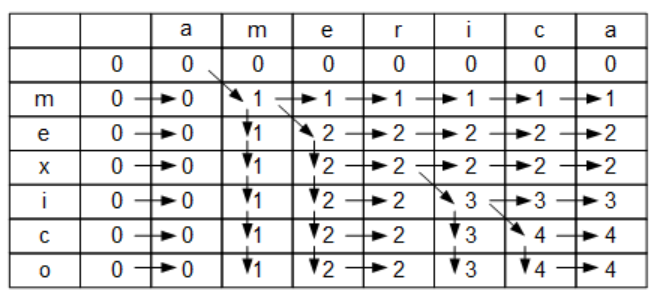
\includegraphics[scale = 0.8]{images/LCS.PNG}
	\caption[Longest Common Sub-sequence]{The value of $C_{ij}$ represents the length of the \textit{LCS} considering the first $i$ characters of the word ''mexico''and the first $j$ characters of the word ''america''.}
	\label{fig:LCS}
\end{figure}

Like in the \textit{LIS}, to know the elements of the \textit{LCS} we just need to keep track of the location where each value comes from. For this case it can come from the element in the left, top, and top-left. The code in \ref{lst:lcs} returns the length of the \textit{LCS} of two strings $X$ and $Y$ with $n$ and $m$ characters respectively.\\

\noindent \textbf{Time Complexity:} $O(nm)$\\
\textbf{Input:}\\
\indent The variables $X, Y, n$ and $m$ are declared as global.\\
\textbf{Output}:\\
\indent The length of the LCS

\begin{lstlisting}[caption={Longest Common Sub-sequence (LCS)}, label={lst:lcs}, numbers=left]
int LCS()
{
    int i, j;
    
    memset(B, 0, sizeof(B));
    memset(C, 0, sizeof(C));

    for(i=1; i<=n; i++)
    {
        for(j=1; j<=m; j++)
        {
            if(X[i-1] == Y[j-1])
            {
                C[i][j] = C[i-1][j-1] + 1;
                B[i][j] = 1;
            }
            else
            {
                if(C[i-1][j] >= C[i][j-1])
                {
                    C[i][j] = C[i-1][j];
                    B[i][j] = 2;
                }
                else
                    C[i][j] = C[i][j-1];
                }
            }
        }

    return C[n][m];
}
\end{lstlisting}

In case we want to print the \textit{LCS} and not just its length, we can use the vector $B$ defined in the code \ref{lst:lcs} to find such sub-sequence. The code in \ref{lst:lcs2} just print one \textit{LCS}, but there can be more than one \textit{LCS} with the same length.\\

\begin{lstlisting}[caption={Printing of the LCS},label={lst:lcs2}, numbers=left]
void LCS_print(int i, int j)
{
    if(i == 0 || j == 0)
        return;
    else
    {
        if(B[i][j] == 1)
        {
            LCS_print(i-1,j-1);
            printf("%d ", X[i-1]);
        }
        else if(B[i][j] == 2)
            LCS_print(i-1,j);
        else
            LCS_print(i,j-1);
    }
}
\end{lstlisting}

\section{Levenshtein Distance (Edit Distance)}

\index{Levenshtein distance} \index{edit distance} Named after Vladimir Levenshtein is a metric for measuring the difference between two sequences. Given two strings of characters \textit{str1} and \textit{str2}, Levenshtein distance is the minimum number of steps needed to transform \textit{str1} into \textit{str2} using three operations.

\begin{itemize}
    \item \textbf{Insertion.} Insert one character in \textit{str1}.
    \item \textbf{Deletion.} Remove one character from \textit{str1}.
    \item \textbf{Replace.} Change one character of \textit{str1} with another.
\end{itemize}

Suppose we want to change the string “LOVE” to “ALONE”. Two operations would be needed.

\begin{enumerate}
    \item Insert $A$ in pisition 0.
    \item Replace $V$ witn $N$.
\end{enumerate}

The algorithm is similar to the one used to find the \textit{Longest Common Sub-sequence}. It is also based on a matrix $C$, where $C_{i,j}$ represents the minimum number of steps to transform the first $i$ characters of \textit{str1} into the first $j$ characters of \textit{str2}. That means that the result will be stored in $C_{n,m}$.\\

The value of $C_{i,j}$ is given by

\begin{equation*}
    C_{i,j} = \min \left (C_{i-1,j-1} + k , \min \left (C_{i,j-1} + 1 , C_{i-1,j} + 1 \right ) \right ),
\end{equation*}

\noindent where $k$ is 1 if $str1_i \neq str2_j$, otherwise is 0.\\

Is also important to initialize the matrix $C$ in the following way

\begin{align*}
    C_{0,0} &= 0 \\
    C_{0,i} &= i, \mbox{ } i=1, \ldots m \\   
    C_{i,0} &= i, \mbox{ } i=1, \ldots n \\   
\end{align*}

If $str1_i = str2_j$ it doesn't represent a cost and $C_{i,j}$ would be equal to $C_{i-1,j-1}$. In case that $str1_i \neq str2_j$ it means that we may need to replace the $i^{th}$ character of $str1$ with $str2_j$  which would we give us a cost of $C_{i-1,j-1} + 1$. In any case we still need to check if it is more convenient to remove character $str_i$ that will have a cost of $C_{i-1,j} + 1$, or insert character $str2_j$ with a cost of $C_{i,j-1} + 1$.\\

To print the operations we just need to keep track of where the value in $C_{i,j}$ comes from. Starting from the element $C_{n,m}$ we need to move backwards, if $C_{i,j} = C_{i-1,j-1}+1$ then is a \textit{replace} operation, if $C_{i,j} = C_{i-1,j}+1$ is a \textit{remove} operation, and if $C_{i,j} = C_{i,j-1}+1$ is an \textit{insert} operation. The code in \ref{lst:edit_distance} reads two strings $str_1$ and $str_2$, and prints the minimum number of operations to turn $str_1$ into $str_2$, and the operations in the order that they must be executed.\\

\noindent \textbf{Time Complexity:} $O(nm)$, where $n$ and $m$ are the length of $str1$ and $str2$ respectively\\
\textbf{Input:}\\
\indent Strings $str1$ and $str2$.\\
\textbf{Output}:\\
\indent The Levenshtein distance of strings $str1$ and $str2$ and the steps to transform $str1$ into $str2$

\begin{lstlisting}[caption={Edit Distance}, label={lst:edit_distance}, numbers=left]
#include <cstdio>
#include <cstring>
#include <algorithm>
#define N 100

using namespace std;

char str1[N], str2[N];
int X[N][N];
int n, m, len;

int Levenshtein_Distance();
void Print_Levenshtein_Distance(int, int);
int min(int, int);

int main()
{
	scanf("%s", str1);
	scanf("%s", str2);

	len = 0;
	n = strlen(str1);
	m = strlen(str2);

	printf("%d\n", Levenshtein_Distance());
	Print_Levenshtein_Distance(n, m);

	return 0;
}
\end{lstlisting}

Following the method described above the function \texttt{Levenshtein\_Distance} computes the minimum number of operations to transform \texttt{str1} into \texttt{str2}. The value of \texttt{X[i][j]} represents the minimum number of steps to transform the sub-string formed by the first $i$ characters of \texttt{str1} into the sub-string formed by the fist $j$ characters of \texttt{str2}. 

\begin{lstlisting}[numbers=left]
int Levenshtein_Distance()
{
	int i, j, k;

	X[0][0] = 0;
	for (i = 1; i <= n; i++)
		X[i][0] = i;

	for (i = 1; i <= m; i++)
		X[0][i] = i;

	for (i = 1; i <= n; i++)
	{
		for (j = 1; j <= m; j++)
		{
			if (str1[i - 1] == str2[j - 1])
				k = 0;
			else
				k = 1;

			X[i][j] = min(min(X[i - 1][j - 1] + k, X[i - 1][j] + 1), X[i][j - 1] + 1);
		}
	}

	return X[n][m];
}
\end{lstlisting}

The function \texttt{Print\_Levenshtein\_Distance} prints the operations needed to transform \texttt{str1} into \texttt{str2} using the values obtained in \texttt{Levenshtein\_Distance}. For each location $(i,j)$ in the matrix is possible to know which operation was made by checking the value of \texttt{X[i][j]} and its neighbors.

\begin{lstlisting}[numbers=left]
void Print_Levenshtein_Distance(int i, int j)
{
	int pos;

	if (i == 0 && j == 0)
		return;

	if (j > 0 && X[i][j - 1] + 1 == X[i][j])
	{
		Print_Levenshtein_Distance(i, j - 1);
		len--;
		pos = i - len;
		printf("Insert %d,%c\n", pos, str2[j - 1]);
	}
	else if (i > 0 && j > 0 && X[i - 1][j - 1] + 1 == X[i][j])
	{
		Print_Levenshtein_Distance(i - 1, j - 1);
		pos = i - len;
		printf("Replace %d,%c\n", pos, str2[j - 1]);
	}
	else if (i > 0 && X[i - 1][j] + 1 == X[i][j])
	{
		Print_Levenshtein_Distance(i - 1, j);
		pos = i - len;
		printf("Delete %d\n", pos);
		len++;
	}
	else if (i > 0 && j > 0)
		Print_Levenshtein_Distance(i - 1, j - 1);
}
\end{lstlisting}

\section{Knapsack Problem}

\index{knapsack problem} Consider the following problem.\\

Is Christmas Eve in Mexico and everyone is out celebrating this special day, you are not the exception and you are in you grandparent’s house eating turkey. Meanwhile a thief gets into your house with the intention to steal different objects. Each object has a specific value and weight; the thief’s knapsack only can carry certain weight. The thief wants to maximize the value of the objects he steal, in other words the thief prefers one object with value of 100 than 99 objects with value of 1. What would be the total maximum value the thief can steal that night? Could you code and algorithm to solve  the thief's dilemma?\\

One approach to this problem using DP consists on using a matrix $C$, where $C_{i,j}$ represents the maximum value the thief can get considering the first $i$ objects and using a knapsack of capacity $j$. In that way the result will be stored in $C_{n,m}$, where $n$ is the number of objects and $m$ is the weight capacity of the knapsack.\\

Each element in the matrix is obtained using the following equation.

\[  C_{i,j} = \left\{
\begin{array}{ll}
      C_{i-1,j} & W_i < j, \\
      \max \left ( C_{i-1,j}, C_{i-1,j-W_i} + V_i\right ) & W_i \geq j,\\
\end{array} 
\right. \]

\noindent where $W_i$ and $V_i$  represents the weight and value of object $i$ respectively.\\

The algorithm stops until the matrix $C$ is filled, making the time complexity of the algorithm equal to the dimensions of $C$, which is $O(nm)$. The algorithm in \ref{lst:knapsack} uses a vector $V$ to store the object values and a vector $W$ to store the object weights and returns the maximum value that can be carried in a knapsack of capacity $m$.\\

\noindent \textbf{Time Complexity:} $O(nm)$, where $n$ is the number of objects and $m$ is the weight the knapsack can carry\\
\textbf{Input:}\\
\indent W: The weight of the objects\\
\indent P: The value of objects\\
\indent n: The number of objects\\
\indent m: The capacity of the knapsack\\
\textbf{Output}:\\
\indent The maximum value the thief can steal

\begin{lstlisting}[caption={Knapsack Problem}, label={lst:knapsack}, numbers=left]
int Knapsack()
{
    long i, j;
    
    memset(C, 0, sizeof(C));

    for(i=1; i<=n; i++)
        for(j=1; j<=m; j++)
            if(W[i] > j)
                C[i][j] = C[i-1][j];
            else
                C[i][j] = max(C[i-1][j], C[i-1][j-W[i]] + V[i]);
                
    return C[n][m];
}
\end{lstlisting}

\section{Maximum Sum in a Sequence}

\index{maximum sum in sequence} Given a sequence of numbers, which can be positive or negative, find a sub-sequence of consecutive elements, which its sum is maximal. For example, consider the following sequence of 10 elements.

$$
-2,\textbf{3,-2,4,4},-8,-5,8,-7,1
$$

The maximum sum that can be obtained is 9, which corresponds to the sub-sequence: 3,-2,4,4. Any other sub-sequence will have a smaller sum.\\

This problem can be solved in linear time by just keeping an accumulated sum of all elements, and when that sum is smaller than zero then reset it to zero. Just be careful with the case where all elements are negatives. In that case the answer is the greatest value. The program in \ref{lst:max_sum} reads $n$ numbers and returns the maximum sum of consecutive elements.\\

\noindent \textbf{Time Complexity:} $O(n)$\\
\textbf{Input:}\\
\indent n: The number of elements in the sequence. Then n integers are given.\\
\textbf{Output}:\\
\indent The maximum sum that can be obtained from a sub-sequence of consecutive elements.

\begin{lstlisting}[caption={Maximum Sum}, label={lst:max_sum}, numbers=left]
#include <stdio.h>
#define oo 1000000

int main()
{
	long i, n, num, s, max;

	scanf("%ld", &n);

	max = -oo;
	s = 0;

	for (i = 0; i<n; i++)
	{
		scanf("%ld", &num);
		if (s + num > 0)
		{
			if (num > s + num)
				s = num;
			else
				s += num;

			if (s > max)
				max = s;
		}
		else
		{
			if (s + num > max)
				max = s + num;
			s = 0;
		}
	}

	printf("The maximum sum is %ld.\n", max);

	while (1);

	return 0;
}
\end{lstlisting}

\section{Rectangle of Maximum Sum}

\index{maximum sum in a rectangle} Given a $n \times n$ matrix of integers, the goal of this algorithm is to find the sub-matrix whose sum of its elements is maximum.\\

The solution proposed here runs in $O(n^3)$, but the idea is the same for the \textit{Maximum Sum} problem, to keep an accumulated sum and reset it when it is smaller than zero. Do it for every column for every sub-matrix.\\

Consider the following matrix.

\begin{figure}[H]
	\centering
	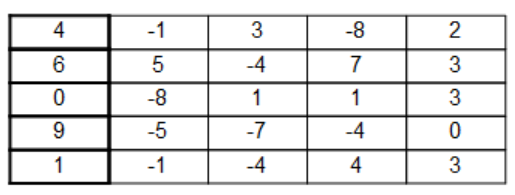
\includegraphics[scale = 0.8]{images/maximum_rectangle.PNG}
	\caption[Rectangle of Maximum Sum]{The matrix can contain positive and negative numbers}
	\label{fig:maximum_rectangle}
\end{figure}

For the matrix in \ref{fig:maximum_rectangle} the maximum sum in a sub-matrix is 20 that corresponds to the sub-matrix formed by the first column. The solution showed in \ref{lst:max_rectangle} receives a square matrix of size $n$ as input, and prints the maximum sum that can be found inside a sub-matrix.\\

\noindent \textbf{Time Complexity:} $O(n^3)$\\
\textbf{Input:}\\
\indent n: The size of the matrix\\
\indent x: The matrix of integers\\
\textbf{Output}:\\
\indent The sum of the elements inside the rectangle of maximum sum

\begin{lstlisting}[caption={Rectangle of Maximum Sum}, label={lst:max_rectangle}, numbers=left]
#include <stdio.h>
#define N 101
#define oo 32767

int x[N][N];
int u[N];

int main()
{
    int i, j, k, n;
    int max;

    scanf("%d", &n);
    for(i=1; i<=n; i++)
    {
        for(j=1; j<=n; j++)
        {
            scanf("%d", &x[i][j]);
            x[i][j] += x[i-1][j];
        }
    }
    
    max = -oo;
    for(i=0; i<n; i++)
    {
        for(j=i+1; j<=n; j++)
        {
            for(k=1; k<=n; k++)
            {
                u[k] = x[j][k] - x[i][k];
                if(u[k-1] > 0)
                    u[k] += u[k-1];

                if(u[k] > max)
                    max = u[k];
            }
        }
    }

    printf("%d\n", max);
    return 0;
}
\end{lstlisting}

\section{Optimal Matrix Multiplication}

\index{optimal matrix multiplication} Given a sequence of $n$ matrices, where the number of rows of matrix $i$ is equal to the number of columns of matrix $i-1$. Our task is to choose the location of open and closed parenthesis in order to minimize the number of multiplications. For example, consider the matrices $A, B$ and $C$ with sizes $5 \times 10, 10 \times 20$ and $20 \times 35$ respectively.\\

If we choose the arrangement $A \times (B \times C)$, the number of multiplications is $8750$. On the other hand, if we choose $(A \times B) \times C$ the number of multiplications is 4500, making this a better solution.\\

We can write the sizes of the matrices in a single vector $A$, where the size of matrix $i$ has size $A_{i-1} \times A_i$, then the number of operations needed to multiply matrix $i$ with matrix $i+1$ is given by $A_{i-1} \times A_i \times A_{i+1}$.\\

The algorithm goes like this. Suppose there is a $n \times n$ matrix $X$, where $X_{i,j}$ represents the minimum number of operations needed to multiply the matrices in the interval $[i,j]$. The idea is to update matrix $X$ in each iteration of the algorithm according to this formula.

\begin{equation}
X_{i,j} = \min \left ( X_{i,j}, X_{i,k} + X_{k+1,j} + A_{i-1} \times A_k \times A_j \right )
\end{equation}

The total number of iterations needed is $n-1$. In the first iteration, segments of length $2$ will be updated, in the second iteration segments of length $3$ will be updated and so on.

\begin{table}[H]
\centering
\begin{tabular}{|c|c|}
\hline
 $X_{1,2},X_{2,3},\ldots , X_{n-1,n}$ &  Values updated in the iteration 1\\
 $X_{1,3},X_{2,4},\ldots , X_{n-2,n}$ &  Values updated in the iteration 2\\
 $\vdots$ & $\vdots$\\
 $X_{1,n}$ &  Values updated in the iteration n-1\\
 \hline
\end{tabular}
\caption[Optimal Matrix Multiplication]{Iterations of the Optimal Matrix Multiplication problem}
\label{tab:tabMatrixMul}
\end{table}

The code in \ref{lst:matrix_multiplication} reads an array $A$ of $n$ elements, $(2 \leq n < 20)$, representing the dimensions of the matrices as explained before, and prints the minimum number of multiplications needed and a representation of how the multiplications should be made.\\

\noindent \textbf{Time Complexity:} $O(n^3)$\\
\textbf{Input:}\\
\indent n: The number of matrices\\
\indent A: The size of the matrices\\
\textbf{Output}:\\
\indent The minimum number of multiplications needed and the sequence of matrices with the parenthesis located in the optimal position.

\begin{lstlisting}[caption={Optimal Matrix Multiplication}, label={lst:matrix_multiplication}, numbers=left]
#include <stdio.h>
#include <string.h>
#define N 20
#define oo 1000000

int X[N][N], S[N][N];
int A[N];
int Matrix_Multiplication(int);

void Print_Sequence(int, int);
int main()
{
    int n, i;
    scanf("%d", &n);
    
    for(i=0; i<n; i++)
        scanf("%d %d", &A[i], &A[i+1]);
    
    printf("%d\n", Matrix_Multiplication(n));
    
    Print_Sequence(1,n);
    printf("\n");

    return 0;
}

int Matrix_Multiplication(int n)
{
    int i, j, k, l, val;
    
    memset(X,0,sizeof(X));
    
    for(l=2; l<=n; l++)
    {
        for(i=1; i<=n-l+1; i++)
        {
            j = i+l-1;
            X[i][j] = oo;
            
            for(k=i; k<=j; k++)
            {
                val = X[i][k] + X[k+1][j] + A[i-1]*A[k]*A[j];
                if(val < X[i][j])
                {
                    X[i][j] = val;
                    S[i][j] = k;
                }
            }
        }
    }

    return X[1][n];
}

void Print_Sequence(int i, int j)
{
    if(i == j)
        printf("A%d", i);
    else
    {
        printf("(");
        Print_Sequence(i,S[i][j]);
        printf(" x ");
        Print_Sequence(S[i][j]+1,j);
        printf(")");
    }
}
\end{lstlisting}

\section{Coin Change Problem}

\index{coin change problem} Given a bottle with an infinite amount of coins of different denominations, in how many ways can you pay a certain amount of money, using just the coins of that bottle?\\

Suppose there are three kinds of coins of 1, 2, 5 cents and we have an infinite amount of them, and we want to know in how many ways we can pay 7 cents. It results that there are 6 ways to pay it.

\begin{itemize}
\item Seven 1 cent coins.
\item Five 1 cent coins and one 2 cents coin.
\item Three 1 cent coins and two 2 cents coins.
\item One 1 cents coin and three 2 cents coins.
\item Two 1 cent coins and one 5 cents coin.
\item One 2 cents coin and one 5 cents coin.
\end{itemize}

Consider the following problem.\\

Mexico's currency consists of \$100, \$50, \$20, \$10, and \$5 notes and \$2, \$1, 50c, 20c, 10c and 5c coins. Program \ref{lst:coin_change} determines for any given amount, in how many ways that amount may be made up. The input consists of a real number no greater than \$300.00. Such amount will be valid, that is will be a multiple of 5c. The Output is a single line consisting of the number of ways in which that amount may be made up.\\

The solution for this problem is similar to the one for the \textit{Knapsack problem}, but this time the number of ways in which $i$ Mexican pesos can be completed by adding coin $k$ to the currency is given by:

\[ X_i = \left\{
\begin{array}{ll}
      1 & i = 0 \\
      X_i & i < k \\
      X_i + X_{i-k} & i \geq k \\
\end{array} 
\right. \]

\noindent notice that in the beginning $X$ must be initialized with zeros.\\

\begin{lstlisting}[caption={Coing Change Problem}, label={lst:coin_change}, numbers=left]
#include <stdio.h>
#include <stdlib.h>
#define N 30001
#define M 11

long long C[M] = {10000,5000,2000,1000,500,200,100,50,20,10,5};
long long X[N];

int main ()
{
    long long i, j, k;
    long long money;
    double num;

    //We can pay 0 dollars in one way
    X[0] = 1;

    for(i=0; i<M; ++i)
    {
        k = C[i];
        for(j=k; j<N; j++)
            X[j] += X[j-k];
    }

    while(scanf("%lf", &num) == 1)
    {
        money = (long long)(num*100.0);
        if(money == 0)
            break;
        
        printf("%lld\n", X[money]);
    }
    
    return 0;
}
\end{lstlisting}

\section{Chapter Notes}

The difficult part in dynamic programming problem is first to realize that it is in fact a dynamic programming problem, and second, to find the recursive formula, because sometimes there is this feeling that a problem has a dynamic programming solution, but is hard to see it. Well the only way to solve this problem is to practice, practice, and practice.\\

There is a section dedicated to dynamic programming in the book \textit{''Introduction to Algorithms''} \cite{cormen}, there we can find a analytic description of some famous problems. Also we recommend to visit the forums of the different online judges, there we can find information and tricks that don't appear in any book.\\

Some online judges have their problems divided by category, bellow there are a couple of links containing only dynamic programming problems.

\begin{itemize}
\item \url{http://acm.timus.ru/problemset.aspx?space=1&tag=dynprog}
\item \url{https://uva.onlinejudge.org/index.php?option=com_onlinejudge&Itemid=8&category=114}
\end{itemize}



\newpage
\section{Exercises}

\begin{tcolorbox}
\begin{enumerate}
    \item How many domino tiles of $2 \times 1$ fit in a $2 \times n$ table for some given $n$? 
    \item A ''bad luck'' number is a number that contains a ''1'' followed by a ''3''. e.g.\ 14137, or 3133. Given a number $n$, write a program that find how many ''bad luck'' numbers of $n$ digits exist?
    \item We have an ice cream shop where we serve three kind of flavors, chocolate, vanilla and strawberry. Our ice cream cones are special, they can be $n$ scoops tall with the constraint that there cannot be two equal flavors together, and that vanilla must be always between chocolate and strawberry. In how many ways can we make a $n$ scoops ice cream cone?
    \item Consider a matrix $A$ of $n \times m$ cells, in how many ways can we get to cell $A_{n,m}$ from cell $A_{1,1}$ if we only can move one cell at a time to the right or up? 
    \item Marie has $n$ coins in her purse, coins can have different values, but she can have more than one coin of the same value. She wants to give \textbf{all} her coins to her two children, but in a way that the difference of what they receive be minimal, in that way any of them will be sad. Write a program that find how many money receive each child.
\end{enumerate}
\end{tcolorbox}

\chapter{Graphs}
\label{chap:graphs}
\begin{chapquote}{Author's name, \textit{Source of this quote}}
``This is a quote and I don't know who said this.''
\end{chapquote}

\textit{Graph Theory} \index{graph theory} is one of the areas with more applications, from image processing to social networks. A graph is no more than nodes or vertices that can be connected by edges, but what they represent is what makes them so important. For example, in a social network every individual can be seen as a node, and if two individuals are friends, then we can connect the corresponding nodes with an edge. Another example can be the cities in a country, each city can be represented as a node, and the roads connecting two cities represents an edge. Figure \ref{fig:graph_intro} shows a graph representing a map, where the countries are the nodes and edges indicate that two countries have a border in common.\\

\begin{figure}[H]
	\centering
	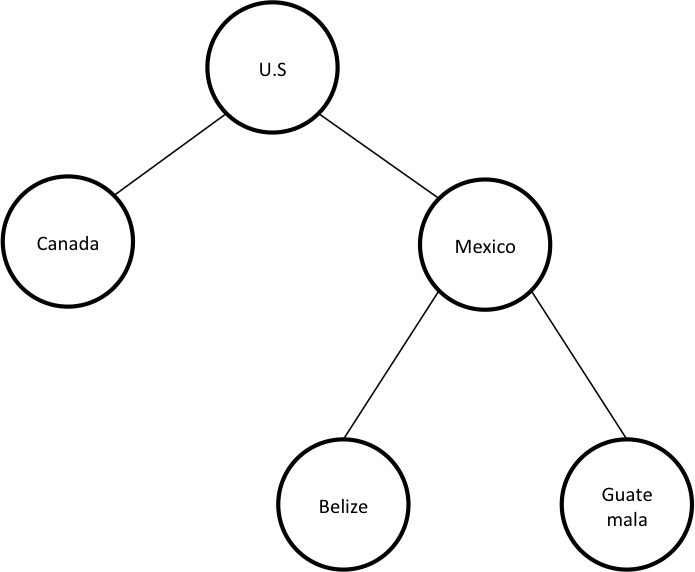
\includegraphics[scale = 0.4]{images/graph_intro.png}
\caption[Graph example]{Graph representing a map, where countries are represented as nodes and edges indicate that two countries share a border.}
\label{fig:graph_intro}
\end{figure}

During this chapter we will see different kind of graphs and learn different algorithms for specific problems, that is why is important to define some concepts about graphs first.\\

As we said, there is more than one kind of graph, and all of them have different properties and applications. Here is a list of the ones we will work with.

\begin{enumerate}
    \item \textbf{Bidirected Graph.} \index{bidirected graph} In this graphs an edge connecting node $a$ with node $b$, is also connecting node $b$ with node $a$. So we can go from $a$ to $b$ and from $b$ to $a$.
    \item \textbf{Directed Graph.} \index{directed graph} Here the edges have a direction, if an edge connects node $a$ with node $b$, then we can go from $a$ to $b$, but not the other way around.
    \item \textbf{Weighted Graph.} \index{weighted graph} For this kind of graphs the edges have a weight or cost associated to it. For example, traveling from New York to Boston has some toll cost, well this can be seen as two nodes (New York and Boston) connected by and edge (road) with a certain cost (toll).
\end{enumerate}

In some cases there can be combinations of different graphs, like a directed and weighted graph, with edges having a direction and a cost. \textbf{Along this chapter we will refer to the number of nodes in a graph with letter $n$, and the number of edges with letter $m$}. Following we list other concepts that are important to know about.

\begin{itemize}
    \item \textbf{Path.} \index{path} It's a series of edges that take us from an initial node to a destination node.
    \item \textbf{Cycle.} \index{cycle} It's a path where the destination node is the same as the initial node.
    \item \textbf{Degree.} \index{node degree} The degree of a node is the number of edges incident to that node.
    \item \textbf{Eulerian Path.} \index{Eulerian path} A path that travels across all the edges in the graph only once.
    \item \textbf{Eulerian Cycle.} \index{Eulerian cycle} A cycle that go through all the edges in the graph only once.
    \item \textbf{Hamiltonian Path.} \index{Hamiltonian path} A path that pass through all the nodes in the graph only once.
    \item \textbf{Hamiltonian Cycle.} \index{Hamiltonian cycle} A cycle that visits all the nodes in the graph only once.
    \item \textbf{Complete Graph.} \index{complete graph} A graph where all nodes are connected directly. A complete graph contains $n(n-1)/2$ edges exactly.
    \item \textbf{Connected Graph.} \index{connected graph} In this graphs there is always a path between any pair of nodes. In other words, it is always possible to reach one node from other node in the graph.
    \item \textbf{Disconnected Graph.} \index{disconnected graph} A graph that is not connected. Meaning that there is at least one pair of nodes $(a,b)$ such that there is no path between node $a$ and node $b$.
    \item \textbf{Cut.} \index{graph cut} A cut is a set of edges that if removed, the vertices are separated in two disjoint sets.
    \item \textbf{Minimum Cut.} \index{graph minimum cut} Is the cut whose sum of the edge weights is minimal.
    \item \textbf{Directed Acyclic Graph (DAG).} \index{DAG. directed acyclic graph} It's a directed graph without cycles, meaning that is impossible to start from any node, follow a path and return to the same node.
\end{itemize}

\section{Graph Traversal}

\index{graph traversal} Two of the most common methods for exploring graphs are the \textit{Depth First Search (DFS)} and the \textit{Breadth First Search (BFS)}. \index{DFS. depth first search} \index{BFS. breadth first search} The first one uses a stack in its implementation, and the other one uses a queue. Both algorithms need a starting vertex in the graph and the adjacent vertexes are added into the stack/queue, then the current vertex is removed and the next is taken, and the vertexes adjacent to it that have not been added are inserted into the data structure. The process continues until all the vertexes has been explored and the stack/queue is empty.

\begin{figure}[H]
	\centering
	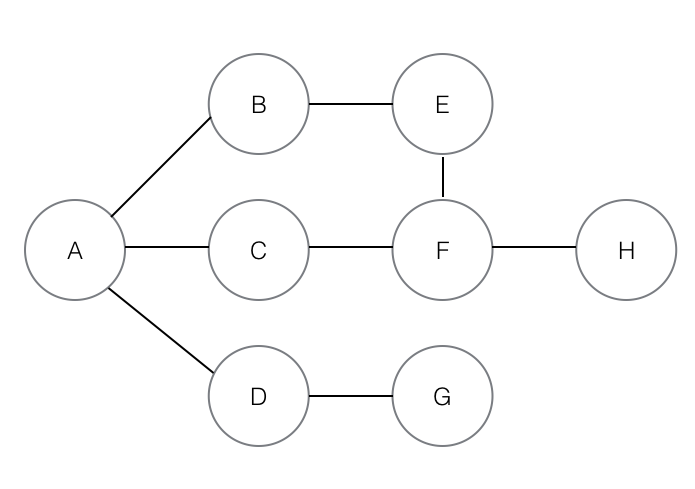
\includegraphics[scale = 0.3]{images/graph1.png}
\caption[Graph Traversal]{The nodes in the graph are visited in different order depending of the algorithm used.}
\label{fig:graph1}
\end{figure}


The difference between these two methods  is that DFS  explores one branch of the graph until it cannot advance no further and then returns and try to explore another branch. On the other hand, BFS explores the graph by levels, first the root, then the vertexes adjacent to the root, then the vertexes adjacent to those vertexes and so on. Let's define the stack for the \textit{DFS} as $S$  and the queue for the \textit{BFS} as $Q$, and using the graph in \ref{fig:graph1} with vertex $A$ as the initial vertex, the graph traversal using both methods is presented in table \ref{table:graph_traversal}. For this case the nodes are inserted into the data structure used in lexicographical order.\\

\begin{table}[H]
\centering
    \begin{tabular}{|l|l|}
    \hline
    \textbf{DFS (stack)} & \textbf{BFS (queue)}\\
    \hline
    $S = [\textcolor{red}{A}]$ & $Q = [\textcolor{red}{A}]$\\
    $S = [\textcolor{red}{D},C,B]$ & $Q = [\textcolor{red}{B},C,D]$\\
    $S = [\textcolor{red}{G},C,B]$ & $Q = [\textcolor{red}{C},D,E]$\\
    $S = [\textcolor{red}{C},B]$ & $Q = [\textcolor{red}{D},E,F]$\\
    $S = [\textcolor{red}{F},B]$ & $Q = [\textcolor{red}{E},F,G]$\\
    $S = [\textcolor{red}{H},E,B]$ & $Q = [\textcolor{red}{F},G]$\\
    $S = [\textcolor{red}{E},B]$ & $Q = [\textcolor{red}{G},H]$\\
    $S = [\textcolor{red}{B}]$ & $Q = [\textcolor{red}{H}]$\\
    $S = []$ & $Q = []$\\
    \hline
    \end{tabular}
\caption[DFS vs. BFS]{Graph Traversal for \textit{DFS} and \textit{BFS}}
\label{table:graph_traversal}
\end{table}

The way in which the traversal is made is different in both algorithms, the nodes in red are the ones that are been explored. For the \textit{DFS} the order on which the vertexes are visited is \textit{A,D,G,C,F,H,E,B}. On the other hand, for the \textit{BFS} the order is \textit{A,B,C,D,E,F,G,H}. So depending on the problem it will be more convenient to use one method then the other, but both of them has the same time complexity.

\subsection{DFS}

\index{DFS. depth first search} The program in \ref{lst:dfs} implements a \textit{DFS} starting from node 0 on a graph $G$ with nodes numbered from $0$ to $n-1$, and prints the nodes as they are visited. The time complexity of the implementation is $O(n^2)$, but if we use an adjacency list instead of an adjacency matrix it runs in $O(n + m)$ time.\\

\noindent \textbf{Time Complexity:} $O(n^2)$\\
\textbf{Input:}\\
\indent Two numbers $n$ $(1 \leq n \leq 100)$,and $m$ $(1 \leq m \leq n(n-1)/2)$, indicating the number of vertices and edges respectively. Then follows $m$ lines, each with two numbers $a$ and $b$, indicating that there is an edge that connects vertex $a$ with vertex $b$, and in the other way around. \\
\textbf{Output}:\\
\indent The nodes that were found by the \textit{DFS} in the order they were visited.

\begin{lstlisting}[caption={DFS}, label={lst:dfs}, numbers=left]
#include <cstdio>
#include <stack>
#include <algorithm>
#define N 101

using namespace std;

stack< int > S;
int G[N][N];    //Adjacency matrix
int V[N];       //Visited nodes
int n, m;       //Number of nodes and edges

void DFS(int);

int main()
{
    int i, a, b;
    
    scanf("%d %d", &n, &m);
    
    for(i=0; i<m; i++)
    {
        scanf("%d %d", &a, &b);
        G[a][b] = G[b][a] = 1;
    }
    
    DFS(0); // Start a DFS from node 0
    
    return 0;
}

void DFS(int a)
{
    int i, v;
    
    V[a] = 1;
    S.push(a);
    
    while(!S.empty())
    {
        v = S.top();    //Get the elemet in the top
        S.pop();        //Remove the top element
        
        printf("%d\n", v);
        
        for(i=0; i<n; i++)
        {
            if(G[v][i] == 1 && V[i] == 0)
            {
                V[i] = 1;
                S.push(i);  //Add ajacent node to the top
            }
        }
    }
}
\end{lstlisting}

\subsection{BFS}

\index{BFS. breadth first search} The code in \ref{lst:bfs} implements a \textit{BFS}, and as we can notice it is almost equal to the code in \ref{lst:dfs}, but instead of using the library \texttt{stack} we use the library \texttt{queue}, and instead of using a stack $S$ we use a queue $Q$. This will cause that every time we execute \texttt{Q.push(a)} the node $a$ will be added at the end to the queue. The input of the program is a graph $G=\{V,E\}$ and prints the nodes as they are visited using node 0 as the initial node.\\

The time complexity is the same as the \textit{DFS}, using an adjacency matrix we obtain more simplicity but also we get a time complexity of $O(n^2)$, which is worst than the $O(n + m)$ we get by using an adjacency list instead.\\

\noindent \textbf{Time Complexity:} $O(n^2)$\\
\textbf{Input:}\\
\indent Two numbers $n$ $(1 \leq n \leq 100)$, and $m$ $(1 \leq m \leq n(n-1)/2)$, indicating the number of vertices and edges respectively. Then follows $m$ lines, each with two numbers $a$ and $b$, indicating that there is an edge that connects vertex $a$ with vertex $b$, and in the other way around.\\
\textbf{Output}:\\
\indent The nodes that were found by the \textit{BFS} in the order they were visited.

\begin{lstlisting}[caption={BFS}, label={lst:bfs}, numbers=left]
#include <cstdio>
#include <queue>
#include <algorithm>
#define N 101

using namespace std;

queue< int > Q;
int G[N][N];    //Adjacency matrix
int V[N];       //Visited nodes
int n, m;       //Number of nodes and edges

void BFS(int);

int main()
{
    int i, a, b;
    
    scanf("%d %d", &n, &m);
    
    for(i=0; i<m; i++)
    {
        scanf("%d %d", &a, &b);
        G[a][b] = G[b][a] = 1;
    }
    
    BFS(0); // Start a BFS from node 0
    
    return 0;
}

void BFS(int a)
{
    int i, v;
    
    V[a] = 1;
    Q.push(a);
    
    while(!Q.empty())
    {
        v = Q.front();  //Get the elemet in the top
        Q.pop();        //Remove the top element
        
        printf("%d\n", v);
        
        for(i=0; i<n; i++)
        {
            if(G[v][i] == 1 && V[i] == 0)
            {
                V[i] = 1;
                Q.push(i);  //Add ajacent node to the bottom
            }
        }
    }
}
\end{lstlisting}

\subsection{Topological Sort}

\index{topological sort} Topological Sort is an application of DFS. Consider a series of tasks that must be accomplished in certain order, for example Suppose there are four tasks: $A, B, C, D$. and $A$ must be accomplished before tasks $C$ and $D$, and task $D$ must be accomplished before task $B$. You need to find a proper order to finish all tasks without breaking any rule. One possible solution is $A D B C$. Meaning that first we finish task $A$, then move to task $D$, then to task $B$, and finally task $C$. That solution doesn't break any constraint. Other solutions are : $A C D B$, and $A D C B$.\\

These rules can be seen as a directed graph, in case that task $A$ comes before of task $B$, there is an edge that goes from node $A$ to node $B$. With the graph representation it is possible to use any of the traversal methods seen so far. For the case of the Topological Sort a \textit{DFS} is needed, and the solution is given by adding into a stack the visited nodes with the condition that each node is added until all their adjacent nodes have been explored.\\

\begin{figure}[H]
	\centering
	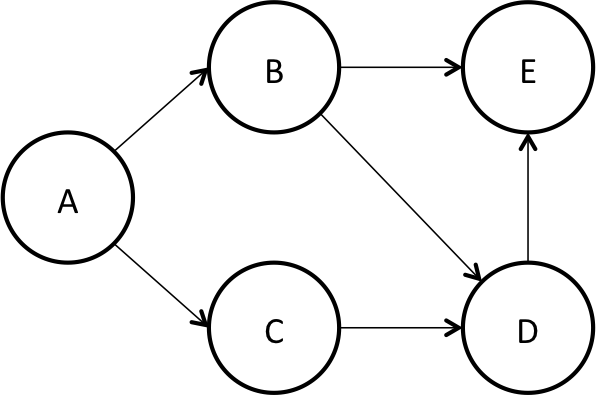
\includegraphics[scale = 0.5]{images/topological.png}
	\caption[Topological Sort]{Directed graph indicating the order in which a set of tasks must be executed. Task $A$ must be executed before task $B$ and task $C$. Task $D$ must be executed after tasks $B$ and $C$, and task $E$ must be executed after tasks $B$ and $D$.}
	\label{fig:topological}
\end{figure}

In the graph \ref{fig:topological} a possible \textit{DFS} traversal can be $ACDEB$, and if each node is added into a stack once all their adjacent nodes have been explored that stack will look like this: $ABCDE$, which is a solution for the Topological Sort problem.\\

The time complexity to find a topological sort in a directed graph is the same for the \textit{DFS}. The program in \ref{lst:topological_sort} stores in stack $S$ a valid topological sort for a given graph $G$.\\

\noindent \textbf{Time Complexity:} $O(n^2)$\\
\noindent \textbf{Input:}\\
    \indent \textbf{n:} Amount of nodes in the graph. $(1 \leq n \leq 100)$.\\
    \indent \textbf{G:} Adjacency matrix of the graph.\\
\noindent \textbf{Output:}\\
    \indent \textbf{S:} Stack with a valid \textit{Topological Sort}.\\

\begin{lstlisting}[caption={Topological Sort}, label={lst:topological_sort}, numbers=left]
#include <stack>
#define N 101

using namespace std;

stack< int > S; //Topological sort
int V[N];       //Visited nodes
int G[N][N];    //Adjacency matrix
int n;          //Number of nodes

void Topological_sort()
{
    int i;

    for(i=0; i<n; i++)
        if(V[i] == 0)
            DFS(i);
}

void DFS(int k)
{
    int i;
    
    V[k] = 1;
    
    for(i=0; i<n; i++)
        if(G[k][i] == 1 && V[i] == 0)
            DFS(i);
    
    S.push(k);
}
\end{lstlisting}

\section{Disjoint Sets}

\index{disjoint sets} For some problems we need to join two sets into a single one and find if a certain element is part of a certain set. If the number of instructions is large, an ordinary graph traversal such as DFS or BFS  is too expensive, so we need something faster.  One of the most popular algorithms is the Union-Find algorithm that will be described ahead.
Union-Find is considered a data structure as well. Basically the structure itself is the solution for the problem that poses if two nodes are in the same connected component. It is a quite simple and elegant structure.\\

Many of the discoveries in the disjoint-set data structures are due to Robert E. Tarjan \cite{union_find}, whom in 1975 found the upper bound of the time complexity for the operations on any disjoint set data structure satisfying certain conditions.\\

\subsection{Union-Find}



\index{union-find algorithm} 
As its name indicates, this algorithm consists on two main steps.

\begin{enumerate}
    \item \textbf{Union.} Joint two sets into a single one.
    \item \textbf{Find.} Determines which set which an element is in.
\end{enumerate}

At the beginning every element is a set. A set can be seen as a tree initially with zero height and with just one node, which is the root. To connect element $a$ with element $b$, we first must find the set of each element, here enters the \textit{Find} operation. Finding the set is equal to finding the root of the tree, if the root is the same for the two elements, then they are already part of the same set. If the root is different then we do the \textit{Union} operation, which consists of merging both trees in a single one. For this we ask for the height of each root and make the root with smaller height child of the root with bigger height. For the case where both roots have the same height any of them can be child of the other, just remember increase the height of the root selected as parent.\\

Consider a graph with 5 nodes and no connections, like the one showed in figure \ref{fig:union-find_1}. Each one of these nodes have a reference to its parent node, which at the beginning is the node itself, and all of them have zero height.

\begin{figure}[H]
	\centering
	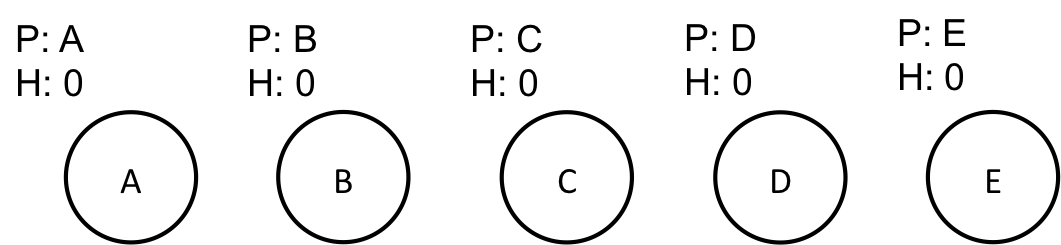
\includegraphics[scale = 0.5]{images/union-find_1.png}
	\caption[Disjoint Sets. Initialization]{At first the parent of each node is the node itself, and all nodes have zero height.}
	\label{fig:union-find_1}
\end{figure}

If we add a connection of node $A$ and node $D$, since both of them have zero height any of them can be the root, for this case $A$ will be the root and it will have a height of 1. If then we connect node $D$ and node $E$, since the root of $D$ is $A$, and $A$ has a larger height than node $E$, then $A$ will be the parent of $E$. See figure \ref{fig:union-find_2}.

\begin{figure}[H]
	\centering
	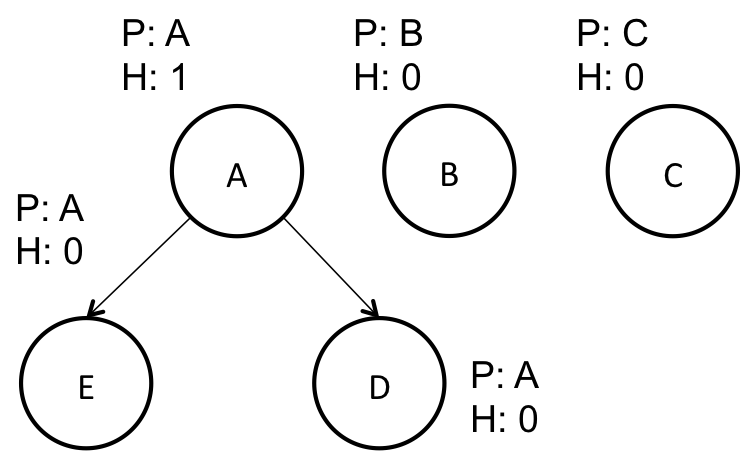
\includegraphics[scale = 0.5]{images/union-find_2.png}
	\caption[Disjoint Sets. Union-Find]{Graph resulting of connecting nodes $A-D$ and $D-E$ using the Union-Find algorithm. Node $D$ and $E$ have node $A$ as their parent, and node $A$ has a height of 1. The directed edge represents a parent-son relationship between nodes.}
	\label{fig:union-find_2}
\end{figure}

One application of the The \textit{Union-Find} is to find the number of Eulerian cycles \index{Eulerian cycle} in a graph which is obtained by \ref{eq:n_eulerian_cycles}.
\begin{equation}
\label{eq:n_eulerian_cycles}
    \#EulerianCycles = 2^k - 1,
\end{equation}

\noindent where $k$ is the number of times a connection of two elements of the same set is created. The algorithm in \ref{lst:union_find} represents a general implementation of the \textit{Union-Find} method, which can be adapted to different applications.\\
 
\noindent \textbf{Time Complexity:}\\
\indent \textit{Union}: $O(1)$\\
\indent \textit{Find}: $O(\log n)$\\
\noindent \textbf{Input:}\\
\indent For every node $x$ added into the graph call the method \texttt{make\_set(x)}.\\
\indent For every connection between two nodes $a$ and $b$ call method \texttt{union\_set(a,b)}.\\
\noindent \textbf{Output:}\\
\indent Depends on the problem, usually the \textit{Union-Find} algorithm is used when there are a large amount of queries.\\


\begin{lstlisting}[caption={Union-Find}, label={lst:union_find}, numbers=left]
#define N 1000

int p[N], rank[N];

void make_set(int x)
{
    p[x] = x;
    rank[x] = 0;
}

void link(int x, int y)
{
    if (rank[x] > rank[y])
        p[y] = x;
    else
    {
        p[x] = y;
        if (rank[x] == rank[y])
            rank[y] = rank[y] + 1;
    }
}

int find_set(int x)
{
    if (x != p[x])
        p[x] = find_set(p[x]);
    
    return p[x];
}

void union_set(int x, int y)
{
    link(find_set(x), find_set(y));
}
\end{lstlisting}

The function \texttt{link} in \ref{lst:union_find} receives two root nodes, $x$ and $y$. The height of node $k$ is stored in \texttt{rank[k]}. If \texttt{rank[x]} is greater than \texttt{rank[y]} then $x$ becomes the parent of $y$. On the other hand, if \texttt{rank[y]} is greater than \texttt{rank[x]} then $y$ becomes the parent of $x$. If both root nodes have the same height any of both nodes can be the parent, so for this case we decided to set $y$ as parent of $x$, that causes that the value of \texttt{rank[y]} increases in one.  

\section{Shortest Paths}

\index{shortest paths} In this section we will cover some of the most popular algorithms to find the shortest path in a graph. These algorithms work for weighted graphs, meaning that edges have a certain weight or cost. A path is a set of edges leading from vertex $A$ to vertex $B$, and the cost of the path is the sum of the weights of all edges that form that path. Then, the shortest path between two nodes is the path with minimum cost. Consider the graph in \ref{fig:shortestpaths1}. Here the cost of the shortest path that leads from node $0$ to node $5$ is $15$, and the path is $0 - 3 - 2 - 5$.

\begin{figure}[H]
	\centering
	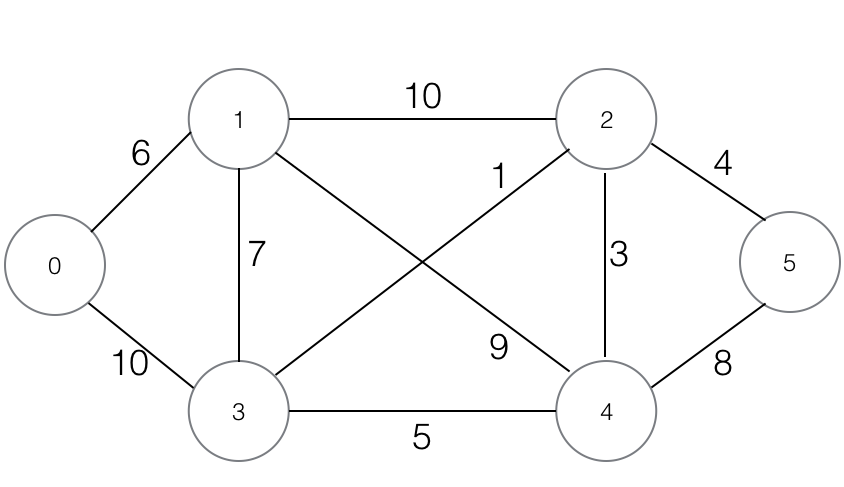
\includegraphics[scale = 0.25]{images/shortestpaths1.png}
	\caption[Weighted Graph]{In a weighted graph edges have a cost associated to it. The cost of a path is the sum of the cost of all edges conforming that path.}
	\label{fig:shortestpaths1}
\end{figure}

\subsection{Dijkstra}

\index{Dijkstra's algorithm} Published by Edsger W. Dijkstra in 1959 \cite{dijkstra}. This algorithm finds the shortest paths between an initial node to all other nodes. Because of its greedy behavior, it only works for positive weights.\\

Given a graph $G$ with $n$ nodes numbered from $0$ to $n-1$, an initial node $a$, and with $G_{ij}=\infty$ if there is no connection between node $i$ and node $j$. The first step is to initialize the distance vector $D$ and visited vector $V$ as follows:

$$
V_i = 0,
D_i=
\begin{cases}
\infty & i \neq a\\
0 & i = a
\end{cases}
$$ 

for every $i$ from $0$ to $n-1$. \\

When $V_i = 1$ we can be sure that the value stored in $D_i$ contains the minimum cost to go from node $a$ to node $i$. The algorithm finds the value of $k$, where $D_k$ is minimum, and $V_k = 0$. Once it is found is marked as visited $(V_k = 1)$ and the value of $D$ is updated using the following formula:

\begin{equation}
D_j = \min \left ( D_j, D_k + G_{kj} \right ), \mbox{ where } V_j = 0
\label{eq:dijkstra1}
\end{equation}

The process is repeated until all nodes are visited or until a value of $k$ can't be found (disconnected graph). At the end the value of $D_i$ stores the minimum cost to go from node $a$ to node $i$. Figure \ref{fig:dijkstra_1} shows every iteration of Dijkstra's algorithm for the graph in \ref{fig:shortestpaths1} with node $0$ as the initial node.\\

\begin{figure}[H]
    \centering
    \subfloat[]{{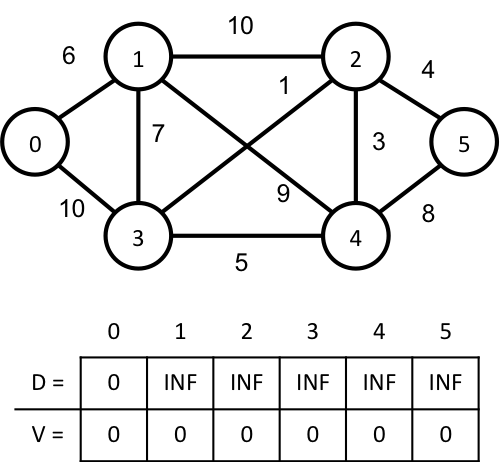
\includegraphics[scale=0.5]{images/dijkstra_1.png} }\label{fig:dijkstra_1_a}} \qquad
    \subfloat[]{{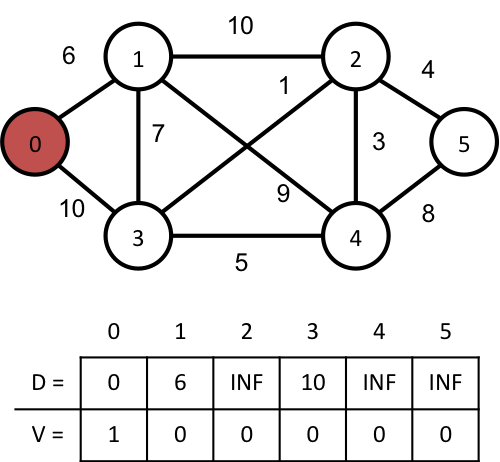
\includegraphics[scale=0.5]{images/dijkstra_2.png} }\label{fig:dijkstra_1_b}} 
\end{figure}
\begin{figure}[H]
    \centering
    \subfloat[]{{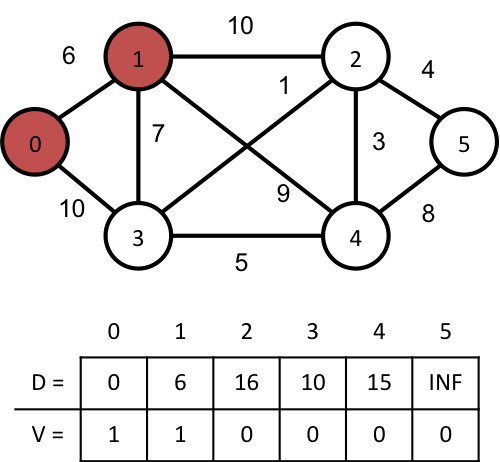
\includegraphics[scale=0.5]{images/dijkstra_3.png} }\label{fig:dijkstra_1_c}} \qquad
    \subfloat[]{{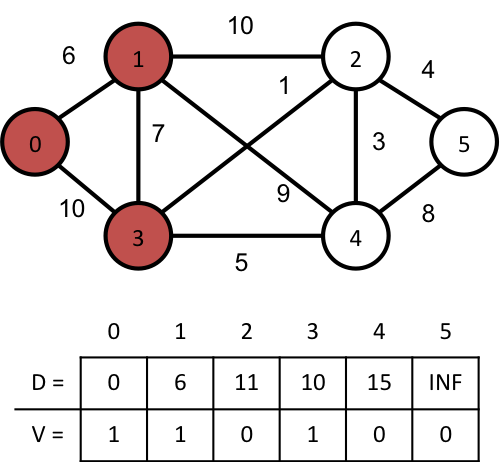
\includegraphics[scale=0.5]{images/dijkstra_4.png} }\label{fig:dijkstra_1_d}} 
\end{figure}
\begin{figure}[H]
    \centering
    \subfloat[]{{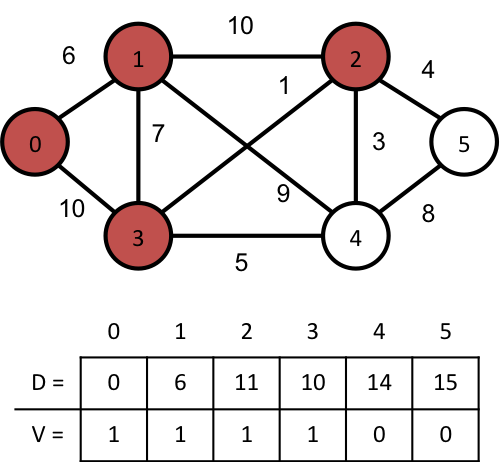
\includegraphics[scale=0.5]{images/dijkstra_5.png} }\label{fig:dijkstra_1_e}} \qquad
    \subfloat[]{{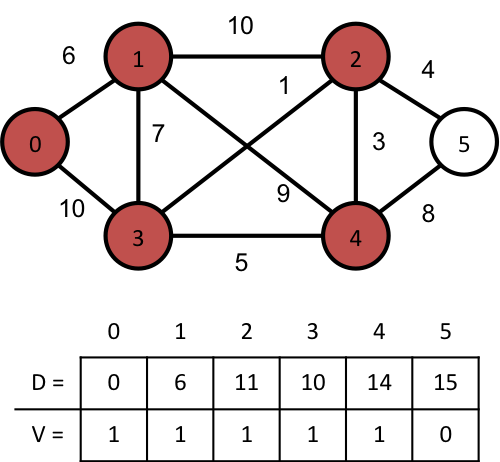
\includegraphics[scale=0.5]{images/dijkstra_6.png} }\label{fig:dijkstra_1_f}} 
\end{figure}
\begin{figure}[H]
    \centering
    \subfloat[]{{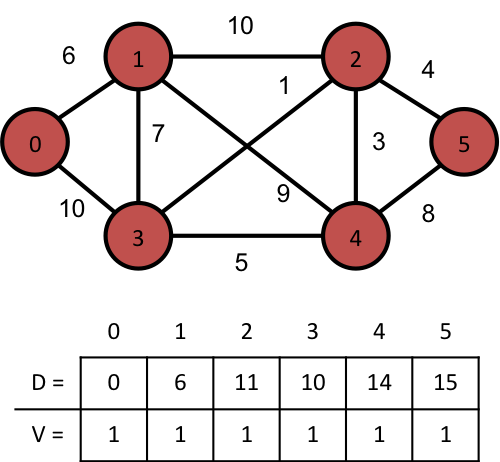
\includegraphics[scale=0.5]{images/dijkstra_7.png} }\label{fig:dijkstra_1_g}}
    \caption[Dijkstra's Algorithm]{Iterations of Dijkstra's algorithm for graph \ref{fig:shortestpaths1} with node $0$ as initial node.}
    \label{fig:dijkstra_1}
\end{figure}

Finding the minimum number in $D$ take $O(n)$ using a \textit{Linear Search}, doing that $n$ times makes the algorithm to run in $O(n^2)$. The code in \ref{lst:dijkstra} implements a generic \textit{Dijkstra} algorithm for a weighted graph $W$ with a given initial node.\\

\noindent \textbf{Time Complexity:} $O(n^2)$\\
\textbf{Input:}\\
\indent $n$. The number of nodes in the graph. $(1 \leq n \leq 100)$.\\
\indent $W$. The matrix of weights.\\
\indent $a$. The initial node. \\
\textbf{Output:}\\
\indent $D$. the minimum cost to reach some node $i$ from node $a$ is stored in $D_i$.

\begin{lstlisting}[caption={Dijkstra}, label={lst:dijkstra}, numbers=left]
#include <algorithm>
#define N 101
#define oo 10000000

using namespace std;

int D[N];       //Array of distances
int V[N];       //Array of visited nodes
int W[N][N];    //Adjacency matrix
int n;          //Number of nodes

void Dijkstra(int a)
{
    int i, j, pos;
    
    for(i=0; i<n; i++)
    {
        D[i] = oo;
        V[i] = 0;
    }
    
    D[a] = 0;
    
    for(i=0; i<n; i++)
    {
        pos = Min_Vertex();
        
        if(pos == -1)   break;
        
        V[pos] = 1;
        
        for(j=0; j<n; j++)
            if(V[j] == 0)
                D[j] = min(D[j], D[pos] + W[pos][j]);
    }
}

int Min_Vertex()
{
    int minVal, pos, i;
    
    minVal = oo;
    pos = -1;
    
    for(i=0; i<n; i++)
    {
        if(V[i] == 0 && D[i] < minVal)
        {
            minVal = D[i];
            pos = i;
        }
    }
    
    return pos;
}
\end{lstlisting}

\subsection{Bellman-Ford}

\index{Bellman-Ford algorithm} The Bellman-Ford algorithm was published in separate works by Richard Bellman \cite{bellman}, and Lester Ford Jr. \cite{ford_fulkerson}. The algorithm finds the cost of the shortest paths from a source vertex to all other vertices. At the contrary of Dijkstra’s Algorithm, this algorithm is capable to handle  negative weights and identify if a negative cycle exists. \\

Using a vector of distances $D$ where $D_i$ represents the minimum cost to travel from the starting node to node $i$. The algorithm goes trough every edge in the graph, if there is an edge that connects node $a$ with node $b$ and has a cost $w$, the vector $D$ us updated as follows:

\begin{equation}
D_b = min(D_b, D_a + w)
\label{eq:edgerelaxation}
\end{equation}

The process is repeated $n$ times for each edge to ensure that the value of $D_i$ contains the minimum cost to go from the initial node to node $i$. The equation \ref{eq:edgerelaxation} is called \textit{edge relaxation}.\\

To verify if there is a negative cycle in the graph an extra relaxation of the edges is made, and if a value of $D$ changes then there is a negative cycle. That happens because in every iteration the algorithm finds a better path by looping in that negative cycle causing the vector $D$ to change every time.\\

\begin{figure}[H]
	\centering
	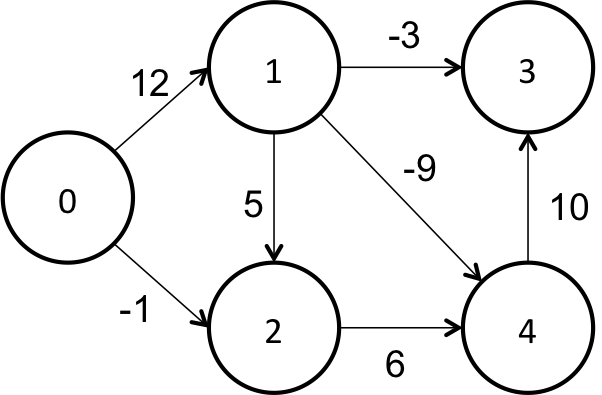
\includegraphics[scale = 0.5]{images/bellman-ford.png}
	\caption[Bellman-Ford]{Directed graph with negative weights.}
	\label{fig:bellman-ford}
\end{figure}

Using the graph defined in \ref{fig:bellman-ford}, to find the minimum cost to travel from node 0 to the rest of the nodes. The distance vector $D$ is initialized as following:

$$
D_i=
\begin{cases}
\infty & i \neq 0\\
0 & i = 0
\end{cases}
$$ 

The next step is to perform the edge relaxation, which can be in any order, for example:

\begin{table}[H]
\centering % used for centering table
\begin{tabular}{c l}
$1 \rightarrow 4$ & $D_4 = \min(\infty, \infty - 9) = \infty-9 = \infty$ \\
$0 \rightarrow 1$ & $D_1 = \min(\infty, 0 + 12) = 12$ \\
$1 \rightarrow 3$ & $D_3 = \min(\infty, 12 - 3) = 9$ \\
$2 \rightarrow 4$ & $D_4 = \min(\infty, \infty + 6) = \infty$ \\
$0 \rightarrow 2$ & $D_2 = \min(\infty, 0 - 1) = -1$ \\
$4 \rightarrow 3$ & $D_3 = \min(9, \infty + 10) = 9$ \\
$1 \rightarrow 2$ & $D_2 = \min(-1, 12 + 5) = -1$ \\
\end{tabular}
\label{table:bellman-ford}
\end{table}

The resulting vector of distances after the edge relaxation is

\begin{table}[H]
\centering % used for centering table
\begin{tabular}{| c | c | c | c | c |}
\hline
$0$ & $12$ & $-1$ & $9$ & $\infty$ \\
\hline
\end{tabular}
\end{table}

To assure that vector $D$ contains the minimum cost to travel from node $0$ to the rest of the nodes, we need to do the edge relaxation at least $n$ times. For this example, with one more edge relaxation is enough and it the vector will look like this:

\begin{table}[H]
\centering % used for centering table
\begin{tabular}{| c | c | c | c | c |}
\hline
$0$ & $12$ & $-1$ & $9$ & $3$ \\
\hline
\end{tabular}
\end{table}

Notice that we must be careful to set the value of $\infty$ at the moment to code the Bellman-Ford algorithm, a small value can return a wrong answer.\\

The edge relaxation runs in $O(m)$ time, and it is performed $n$ times, which makes the time complexity of the algorithm to be $O(nm)$. The Bellman-Ford algorithm is showed in \ref{lst:bellman_ford}, and it uses an array $E$ to store the edges in the graph. The program returns $1$ if there is a negative cycle, otherwise return 0. \\

\noindent \textbf{Time Complexity:} $O(nm)$\\
    \indent $n$. Number of nodes. $(1 \leq n \leq 100)$\\
    \indent $m$. Number of edges.\\
\textbf{Input:}\\
\indent $E$. Array of  edges.\\
\indent $src$. The initial node. \\
\textbf{Output:}\\
\indent $D$. the minimum cost to reach some node $i$ from node \texttt{src} is stored in $D_i$. If there is a negative cycle the function \texttt{Bellman\_Ford} returns 1.\\

\begin{lstlisting}[caption={Bellman-Ford}, label={lst:bellman_ford}, numbers=left]
#define N 101
#define oo 10000000

class Edge
{
public:
    int u;
    int v;
    int w;
    
    Edge(int u = 0, int v = 0, int w = 0)
    {
        this->u = u;
        this->v = v;
        this->w = w;
    }
};

Edge E[N*N];    //Array of edges
int D[N];       //Array of distances
int n, m;       //Number of nodes and edges

int Bellman_Ford(int src)
{
    int i, j, u, v, w;
    
    for(i=0; i<n; i++)
        D[i] = oo;
    D[src] = 0;
    
    for(i=0; i<n-1; i++)
    {
        for(j=0; j<m; j++)
        {
            u = E[j].u;
            v = E[j].v;
            w = E[j].w;
            
            if(D[v] > D[u] + w)
                D[v] = D[u] + w;
        }
    }
    
    for(j=0; j<m; j++)
    {
        u = E[j].u;
        v = E[j].v;
        w = E[j].w;
        
        if(D[v] > D[u] + w)
            return 1;           //Negative cycle!!
    }
    
    return 0;                   //No negative cycles
}
\end{lstlisting}

\subsection{Floyd-Warshall}

\index{Floyd-Warhall algorithm} Described by Robert Floyd \cite{floyd}, who based it on the work of Stephen Warshall \cite{warshall}. The Floyd-Warshall algorithm  is used  to  find  the cost of the  shortest  paths  between  all  pair  of  vertices, which are  stored  in  the  same  weighted  adjacency  matrix  W.  This  algorithm  works for positive and negative weights. Is important to notice that the time complexity of this algorithm makes it very hard to use it for real applications, and is recommended to use it in graphs with small number of vertices. \\

The idea behind the Floyd-Warshall's algorithm is to update constantly the the minimum cost to get from some node $i$ to another node $j$ using as intermediate point some node $k$, where $k$ takes values from $0$ to $n-1$.\\   

One advantage of this algorithm is that is easy to implement, just three nested loops and the matrix of weights is what it needs. See the code \ref{lst:floyd}.\\

\noindent \textbf{Time Complexity:} $O(n^3)$\\
\noindent \textbf{Input:}\\
\indent n. The number of nodes.\\
\indent W. Matrix of weights.\\
\noindent \textbf{Output:}\\
\indent W. The minimum cost to go from some node $i$ to another node $j$ is stored in $W_{ij}$.\\

\begin{lstlisting}[caption={Floyd-Warshall}, label={lst:floyd}, numbers=left]
void Floyd_Warshall()
{
    int i, j, k;
    
    for(k=0; k<n; k++)
        for(i=0; i<n; i++)
            for(j=0; j<n; j++)
                W[i][j] = min(W[i][j], W[i][k] + W[k][j]);
}
\end{lstlisting}

Figure \ref{fig:floyd-warshall} shows how the matrix of weights $W$ change for every value of $k$ in Floyd-Warshall's algorithm using the graph in \ref{fig:bellman-ford}.

\begin{figure}[H]
\centering % used for centering table
\subfloat[Original matrix of weights]
{
    \begin{tabular}{| c | c | c | c | c |}
    \hline
    $0$ & $12$ & $-1$ & $\infty$ & $\infty$ \\
    \hline
    $\infty$ & $0$ & $5$ & $-3$ & $-9$ \\
    \hline
    $\infty$ & $\infty$ & $0$ & $\infty$ & $6$ \\
    \hline
    $\infty$ & $\infty$ & $\infty$ & $0$ & $\infty$ \\
    \hline
    $\infty$ & $\infty$ & $\infty$ & $10$ & $0$ \\
    \hline
    \end{tabular}
} \qquad
\subfloat[$k=0$. There is no edge from any node to node $0$, so the matrix remains the same.]
{
    \begin{tabular}{| c | c | c | c | c |}
    \hline
    $0$ & $12$ & $-1$ & $\infty$ & $\infty$ \\
    \hline
    $\infty$ & $0$ & $5$ & $-3$ & $-9$ \\
    \hline
    $\infty$ & $\infty$ & $0$ & $\infty$ & $6$ \\
    \hline
    $\infty$ & $\infty$ & $\infty$ & $0$ & $\infty$ \\
    \hline
    $\infty$ & $\infty$ & $\infty$ & $10$ & $0$ \\
    \hline
    \end{tabular}
}\\
\end{figure}
\begin{figure}[H]
\centering % used for centering table
\subfloat[$k=1$. Nodes $3$ and $4$ can be reached from node $0$ passing trough node $1$.]
{
    \begin{tabular}{| c | c | c | c | c |}
    \hline
    $0$ & $12$ & $-1$ & $9$ & $3$ \\
    \hline
    $\infty$ & $0$ & $5$ & $-3$ & $-9$ \\
    \hline
    $\infty$ & $\infty$ & $0$ & $\infty$ & $6$ \\
    \hline
    $\infty$ & $\infty$ & $\infty$ & $0$ & $\infty$ \\
    \hline
    $\infty$ & $\infty$ & $\infty$ & $10$ & $0$ \\
    \hline
    \end{tabular}
} \qquad
\subfloat[$k=2$. Crossing trough node $2$ doesn't led us to a better solution, so the matrix remains without change.]
{
    \begin{tabular}{| c | c | c | c | c |}
    \hline
    $0$ & $12$ & $-1$ & $9$ & $3$ \\
    \hline
    $\infty$ & $0$ & $5$ & $-3$ & $-9$ \\
    \hline
    $\infty$ & $\infty$ & $0$ & $\infty$ & $6$ \\
    \hline
    $\infty$ & $\infty$ & $\infty$ & $0$ & $\infty$ \\
    \hline
    $\infty$ & $\infty$ & $\infty$ & $10$ & $0$ \\
    \hline
    \end{tabular}
}\\
\end{figure}
\begin{figure}[H]
\centering % used for centering table
\subfloat[$k=3$. Node $3$ cannot be an intermediate node because there is no edge coming out from it. The matrix remains the same.]
{
    \begin{tabular}{| c | c | c | c | c |}
    \hline
    $0$ & $12$ & $-1$ & $9$ & $3$ \\
    \hline
    $\infty$ & $0$ & $5$ & $-3$ & $-9$ \\
    \hline
    $\infty$ & $\infty$ & $0$ & $\infty$ & $6$ \\
    \hline
    $\infty$ & $\infty$ & $\infty$ & $0$ & $\infty$ \\
    \hline
    $\infty$ & $\infty$ & $\infty$ & $10$ & $0$ \\
    \hline
    \end{tabular}
} \qquad
\subfloat[$k=4$. Going from node $2$ to node $3$ has a cost of 16 if we pass trough node $4$.]
{
    \begin{tabular}{| c | c | c | c | c |}
    \hline
    $0$ & $12$ & $-1$ & $9$ & $3$ \\
    \hline
    $\infty$ & $0$ & $5$ & $-3$ & $-9$ \\
    \hline
    $\infty$ & $\infty$ & $0$ & $16$ & $6$ \\
    \hline
    $\infty$ & $\infty$ & $\infty$ & $0$ & $\infty$ \\
    \hline
    $\infty$ & $\infty$ & $\infty$ & $10$ & $0$ \\
    \hline
    \end{tabular}
}\\
\caption[Floyd-Warshall]{Matrix of weights for different values of $k$ in the Floyd-Warshall algorithm. The first row is equal to the resulting vector of distances in the Bellman-Ford algorithm.}
\label{fig:floyd-warshall}
\end{figure}

\subsection{A*}

\index{A* algorithm} First described by Peter Hart, Nils Nilsson, and Bertram Raphael in 1968 \cite{a_star}. The A-star is an heuristic algorithm that is used to find the shortest path to go from some node $A$ to some other node $B$. It is particular useful when memory or time constraints make hard to use the other algorithms seen so far.\\

The idea of the algorithm is to explore in every iteration the node with less cost associated to it. The cost of a given node $k$ is define by:

\begin{equation}
    f(k) = g(k) + h(k) ,
\label{eq:astar1}
\end{equation}

where $g(k)$ is the accumulated cost so far until reaching node $k$, and $h(k)$ is an \textbf{optimistic} guess of the cost needed to reach the destination node from node $k$, meaning that if $d(k)$ the minimum cost to travel from  node $k$ to the destination node, then we must assure that $h(k) \leq d(k)$.\\

We must be very careful when choosing the heuristic function $h$, a wrong function will lead us to an incorrect result. This function depends on the problem to solve. For example, in the case of grid with obstacles where the goal is to reach some specific cell, starting from another cell just moving up, down, left and right. One possible heuristic function is to return the Manhattan distance between the current cell and the destination cell. \\

The code in \ref{lst:a_star} reads two numbers $n$ ad $m$, that represents the number of nodes and edges in the graph respectively. $m$ lines follow, each one containing three numbers $a,b$, and $k$, indicating that there is an edge with cost $k$ connecting nodes $a$ and $b$. Finally two more numbers are given indicating the initial and destination nodes respectively. The program prints the minimum cost to travel from the initial node to the destination node using the A* algorithm.\\   

The class \texttt{Node} contains three attributes, \texttt{v} that refers to the node index, \texttt{g} that indicates the cost of reaching node \texttt{v} from the initial node, which represents the current cost. The value of \texttt{f} is an optimistic estimate of what will cost us to reach the destination. Since we use a priority queue to get the node with less value of \texttt{f} we need to overload any of the operators \texttt{<} \texttt{>}. 

\begin{lstlisting}[caption={A-star}, label={lst:a_star}, numbers=left]
#include <iostream> 
#include <list> 
#include <vector> 
#include <queue>
#define oo 1000000 

using namespace std;

class Node
{
public:
    int v;
    int g;
    int f;
    Node()
    {
    }
    Node(int v, int g, int f)
    {
        this->v = v;
        this->g = g;
        this->f = f;
    }
    
    bool operator < (const Node &node) const
    {
        return this->f > node.f;
    }
    
    bool operator > (const Node &node) const
    {
        return this->f < node.f;
    }
};

int nVertex, nEdges;
vector< list <Node> > G;
vector< int > h;
priority_queue<Node> L;

void A_Star(int, int);

int main()
{
    int i, k;
    int a, b;
    int src, dst;
    
    cin >> nVertex >> nEdges;
    G.resize(nVertex);
    h.resize(nVertex);
    
    for(i=0; i<nEdges; i++)
    {
        cin >> a >> b >> k;
        
        if(h[a] == 0)
            h[a] = k;
        else
            h[a] = min(h[a], k);
        
        G[a].push_back(Node(b, k, 0));
    }
    
    cin >> src >> dst;
    A_Star(src, dst);
    
    return 0;
}
\end{lstlisting}

The function \texttt{A\_Star} implements the \textit{A*} algorithm given the source and destination nodes. The nodes are added to a priority queue, and in each iteration the element at the top is selected, which represent the node with less cost. The heuristic for some node $k$ used in this exercise is the minimum cost between all edges connected to $k$.

\begin{lstlisting}[numbers=left]
void A_Star(int src, int dst)
{
    int u;
    int v, g, f;
    
    Node nodeA, nodeB;
    list<Node>::iterator it;
    
    u = src;
    h[dst] = 0;
    L.push(Node(src, 0, 0));
    
    nodeA = L.top();
    L.pop();
    do
    {
        cout << "Node : " << u << " f = " << nodeA.f << endl;
        
        for(it = G[u].begin(); it != G[u].end(); it++)
        {
            nodeB = *it;
            v = nodeB.v;
            g = nodeA.g + nodeB.g;
            f = g + h[v];
            L.push(Node(v, g, f));
        }
        
        nodeA = L.top();
        L.pop();
        u = nodeA.v;
    }
    while(u != dst);
    
    cout << nodeA.f << endl;
}
\end{lstlisting}

\section {Strongly Connected Components}

\index{strongly connected components} A strongly connected component (SCC) in a graph is a subgraph where all its nodes are connected directly or indirectly, thus we can reach any node from any other node. For figure \ref{fig:scc} there are four SCC's, one formed by nodes $\{ 0,1,2,3,5 \}$, other formed by $\{ 4,6 \}$, and two more formed by a single node $\{ 7 \}$, and $\{ 8 \}$.\\

\begin{figure}[H]
	\centering
	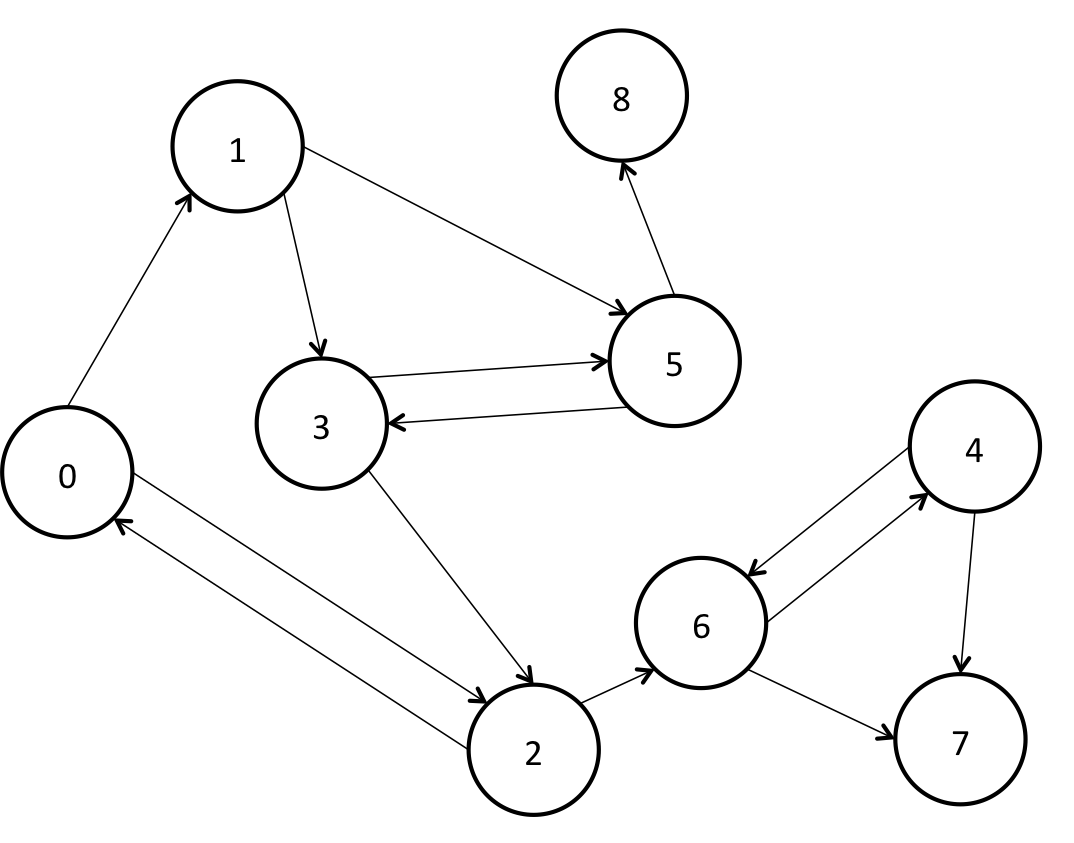
\includegraphics[scale = 0.4]{images/scc_1.png}
	\caption[Strongly Connected Components]{Directed graph with cycles.}
	\label{fig:scc}
\end{figure}

If all SCC's are seen as individual nodes, we can convert a cyclic graph in a DAG (directed acyclic graph). In this section we will review two algorithms that find the strongly connected components in a graph, Tarjan's algorithm and Kosaraju's algorithm, both based in \textit{DFS}. 

\subsection{Tarjan's Algorithm}

\index{Tarjan's algorithm} Invented by Robert Tarjan in 1972 \cite{tarjan} and based on a \textit{DFS}. Tarjan's algorithm finds the strongly connected components and cycles in a \textbf{directed graph}. The complexity of the algorithm is the same for the \textit{DFS} $O(n + m)$. If we use an adjacency matrix as in the code in \ref{lst:tarjan}, the time complexity is $O(n^2)$.\\

As nodes are visited in the \textit{DFS}, they are added to a stack $L$ and enumerated, this way each node $v$ will have an index or identifier $S_v$. Each node $v$ also needs to keep track of the node with the smallest index that is reachable from $v$, including $v$ itself, we will call it $low_v$. Once all adjacent nodes of $v$ have been explored, and if $low_v$ is equal to $S_v$, then we can be sure that there is a cycle, and all nodes added to $L$ after $v$ are part of the same SCC. Remove all the elements of the SCC from $L$ and continue with the search.\\

The time complexity of the algorithm is the same as the \textit{DFS}, but needs more memory to store the values of $S_i$ and $low_i$ for each $i=0, \ldots, n-1$. The algorithm is implemented in \ref{lst:tarjan}\\

\noindent \textbf{Time Complexity:} $O(n^2)$\\
\textbf{Input:}\\
\indent $n$. The number of nodes. $(1 \leq n \leq 100)$.\\
\indent $G$. The adjacency matrix.\\
\textbf{Output:}\\
\indent Prints the strongly connected components of $G$\\

\begin{lstlisting}[caption={Tarjan Algorithm}, label={lst:tarjan}, numbers=left]

#include <algorithm>
#define N 101

using namespace std;

int G[N][N];
int S[N], LOW[N], L[N], R[N];
int n, nVertex, nComponents;

void Tarjan()
{
    for(int i=0; i<n; i++)
    {
        if(S[i] == -1)
        {
            nVertex = 0;
            nComponents = 0;
            DFS(i);
        }
    }
}

void DFS(int v)
{
    int k;
    
    S[v] = nVertex++;
    LOW[v] = S[v];
    L[nComponents++] = v;
    R[v] = 1;
    
    for(int i=0; i<n; i++)
    {
        if(G[v][i] == 1)
        {
            if(S[i] == -1)
            {
                DFS(i);
                LOW[v] = min(LOW[v],LOW[i]);
            }
            else if(R[i] == 1)
                LOW[v] = min(LOW[v],S[i]);
        }
    }
    
    if(S[v] == LOW[v])
    {
        printf("SCC:\n");
        do
        {
            k = L[nComponents-1];
            R[k] = 0;
            nComponents--;
            printf("%d\n", k);
        }
        while(k != v && nComponents > 0);
    }
}
\end{lstlisting}

Figure \ref{fig:tarjan} shows how the values of $S_v$ and $low_v$ change trough the \textit{DFS} for the graph in \ref{fig:scc}.

\begin{figure}[H]
    \centering
    \subfloat[\tiny{$L = \{ 0 \}$. Start the \textit{DFS} from node $0$.}  ]{{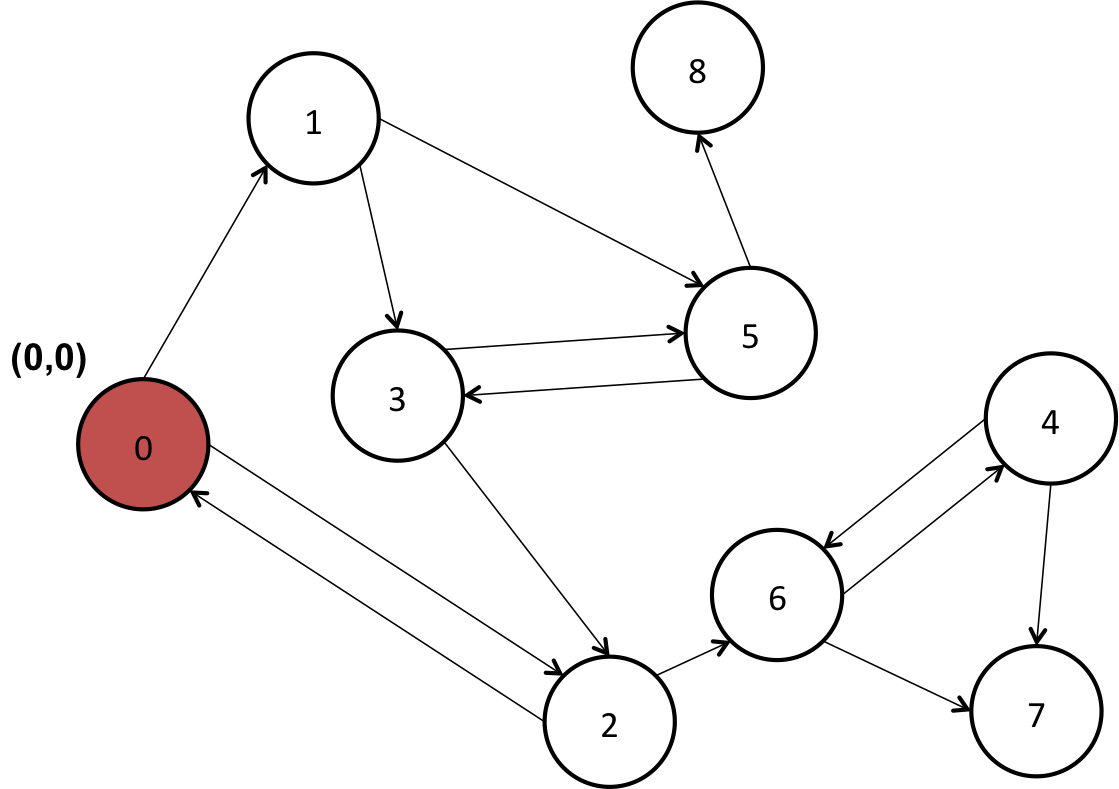
\includegraphics[scale=0.25]{images/tarjan_1.png} }\label{fig:tarjan_1_a}} \qquad
    \subfloat[\tiny{$L = \{ 0,1 \}$. Visit node $1$.}]{{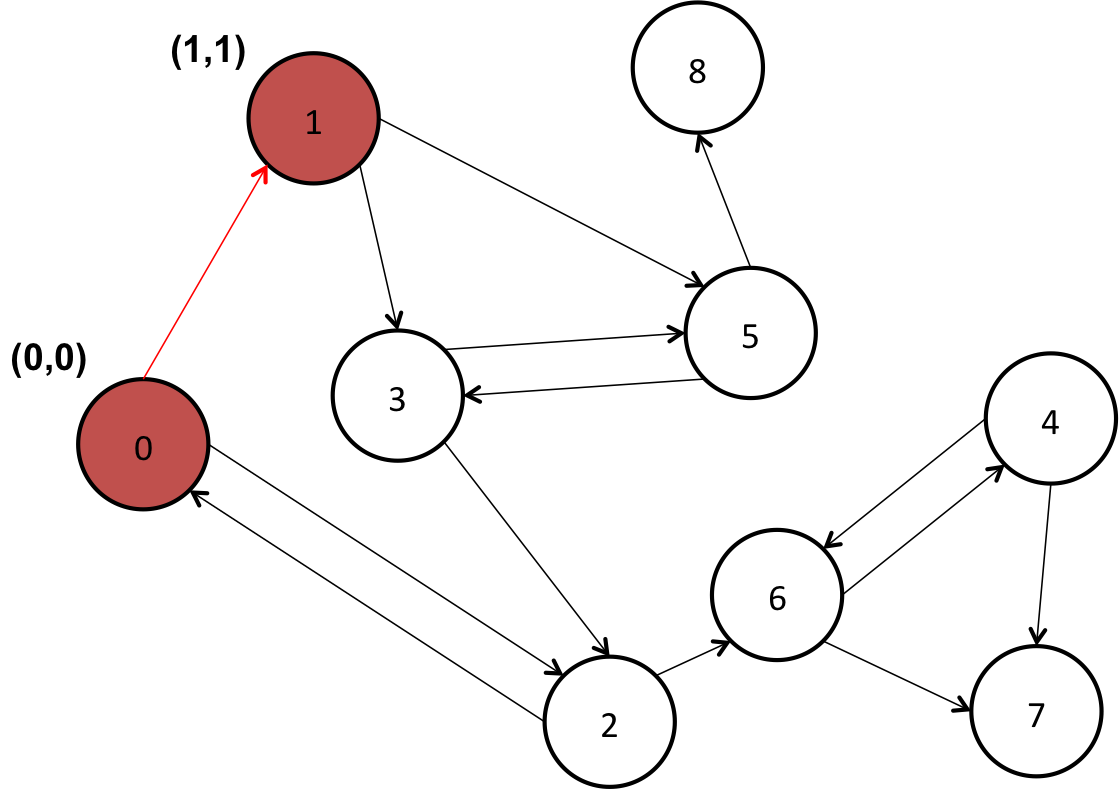
\includegraphics[scale=0.25]{images/tarjan_2.png} }\label{fig:tarjan_1_b}} \\
\end{figure}
\begin{figure}[H]
    \centering
    \subfloat[\tiny{$L = \{ 0,1,3 \}$. Visit node $3$.}]{{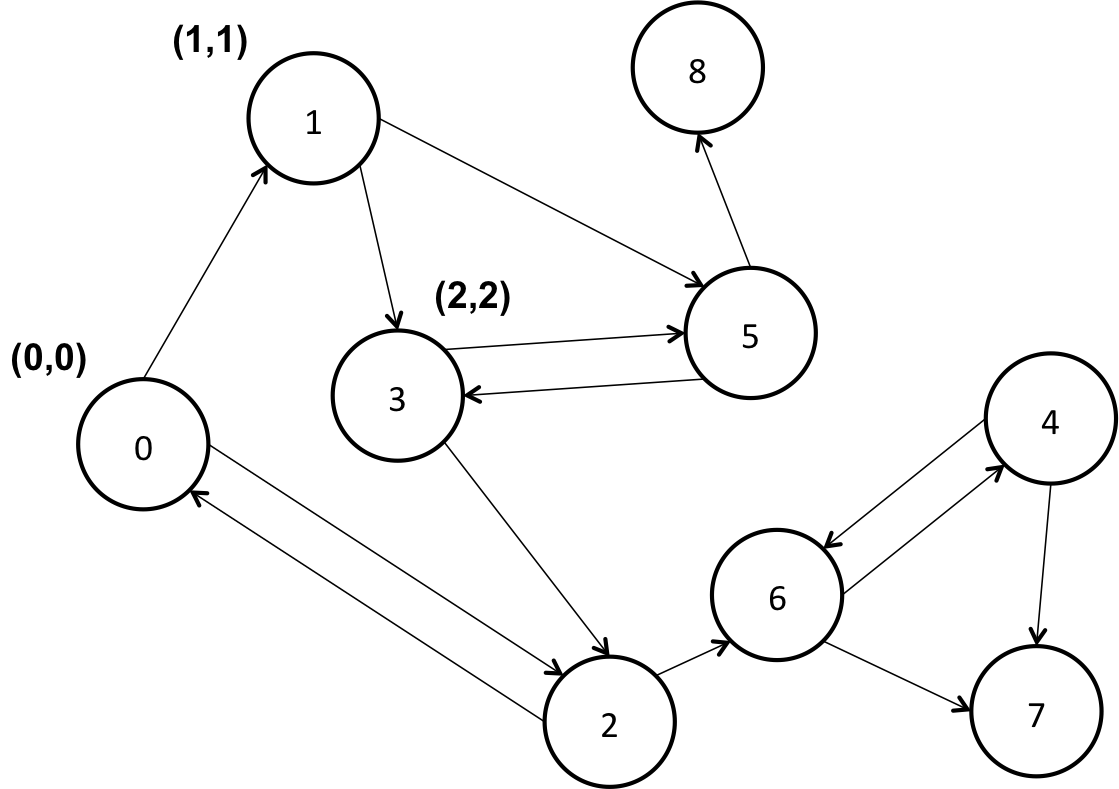
\includegraphics[scale=0.25]{images/tarjan_3.png} }\label{fig:tarjan_1_c}} \qquad
    \subfloat[\tiny{$L = \{ 0,1,3,2 \}$. Visit node $2$.}]{{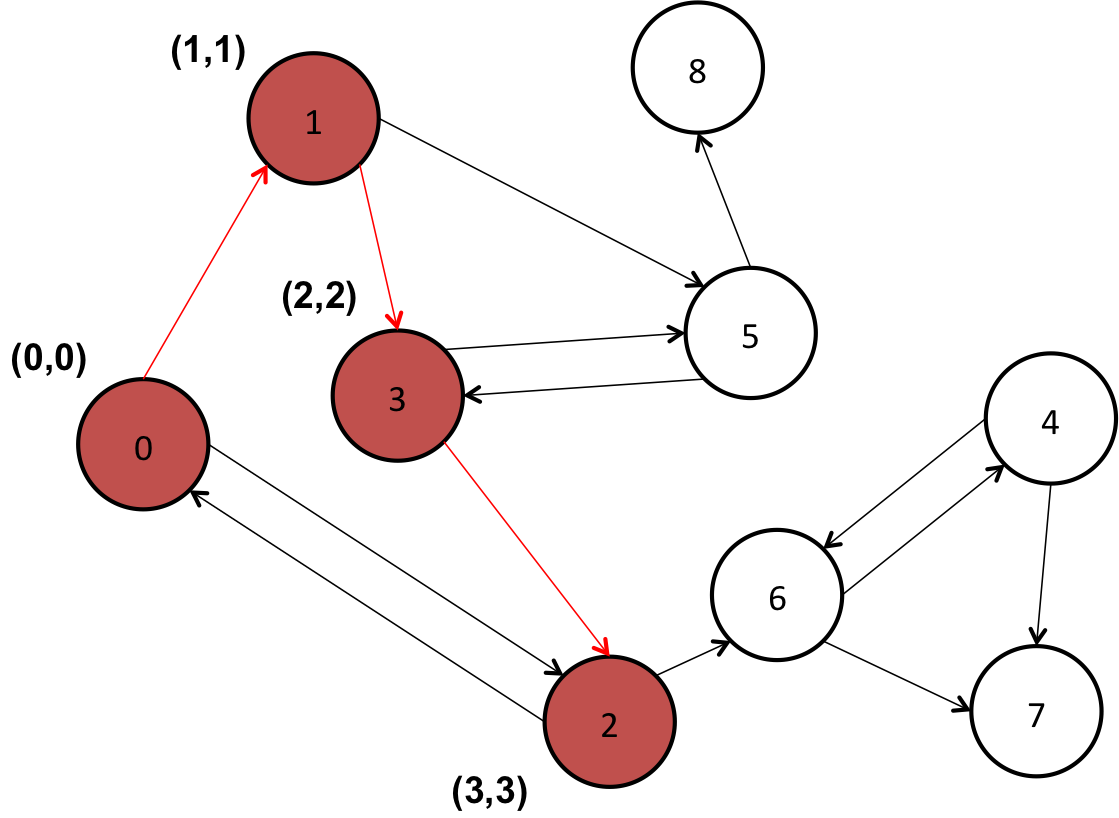
\includegraphics[scale=0.25]{images/tarjan_4.png} }\label{fig:tarjan_1_d}} \\
\end{figure}
\begin{figure}[H]
    \centering
    \subfloat[\tiny{$L = \{ 0,1,3,2 \}$. $low_2=0$ because node $2$ is connected to the node with index $0$.}]{{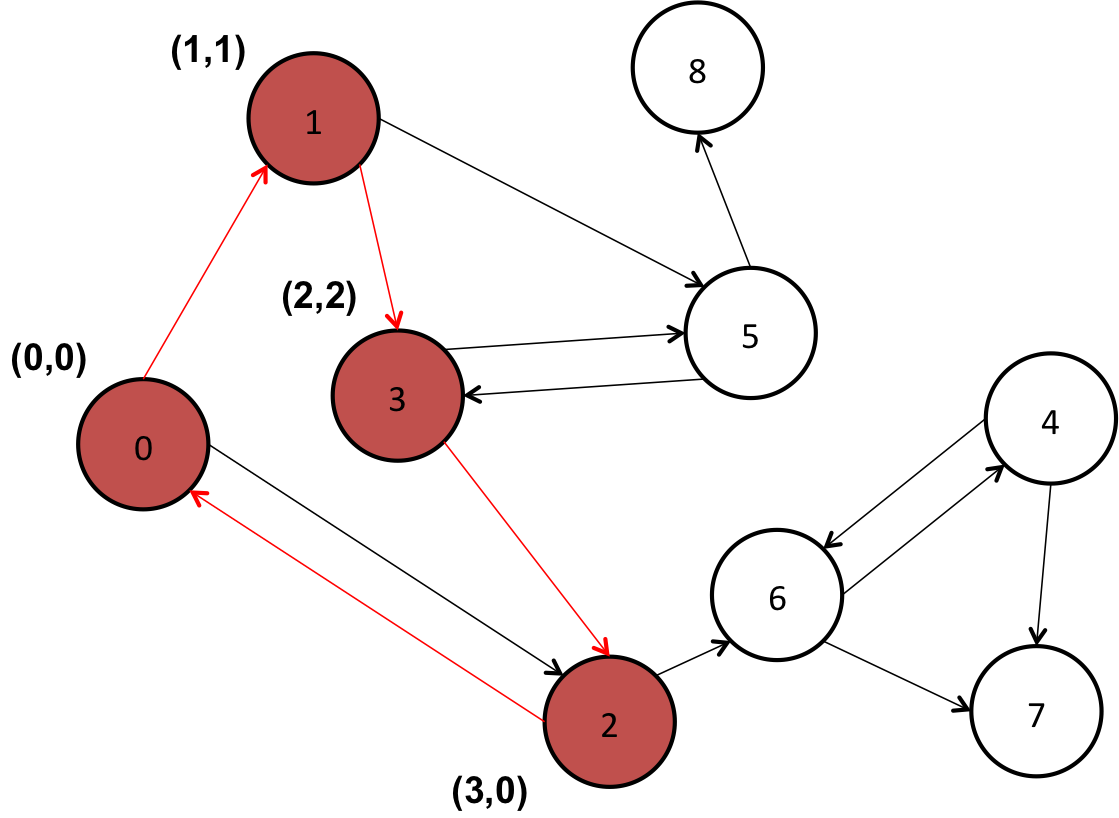
\includegraphics[scale=0.25]{images/tarjan_5.png} }\label{fig:tarjan_1_e}} \qquad
    \subfloat[\tiny{$L = \{ 0,1,3,2,6\}$. Visit node $6$.}]{{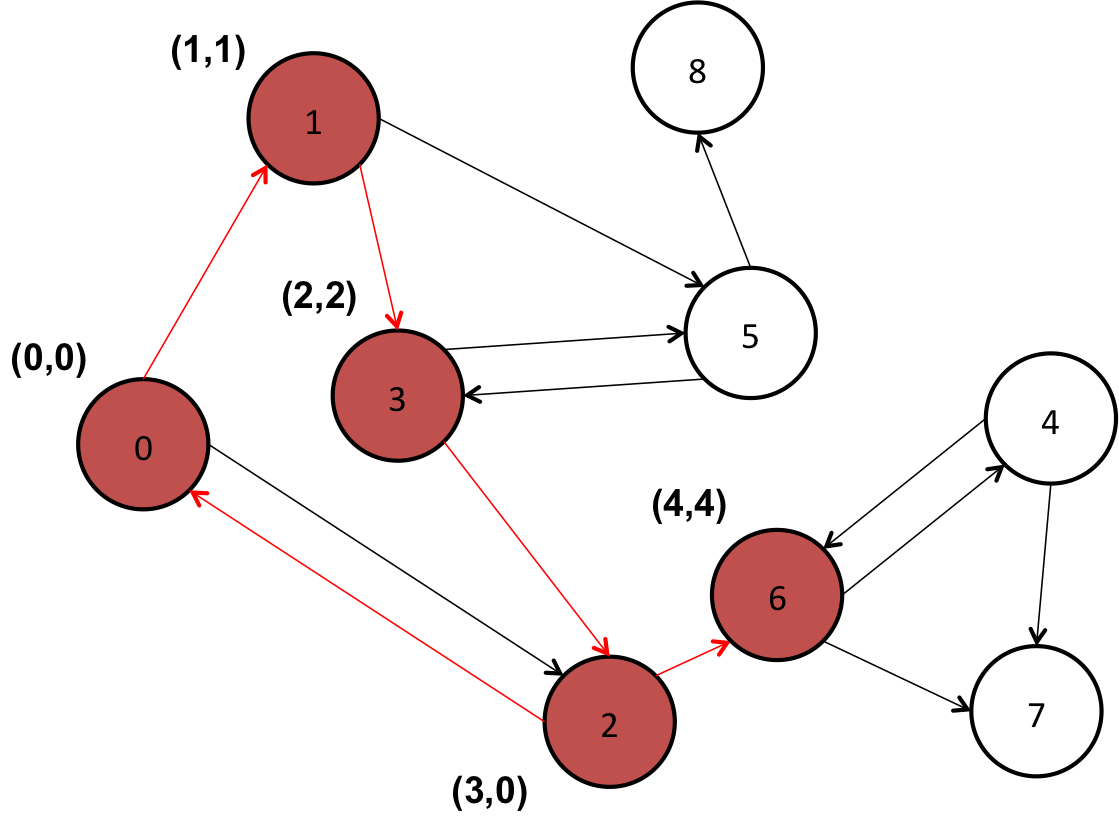
\includegraphics[scale=0.25]{images/tarjan_6.png} }\label{fig:tarjan_1_f}} \\
\end{figure}
\begin{figure}[H]
    \centering
    \subfloat[\tiny{$L = \{ 0,1,3,2,6,4\}$. Visit node $4$.}]{{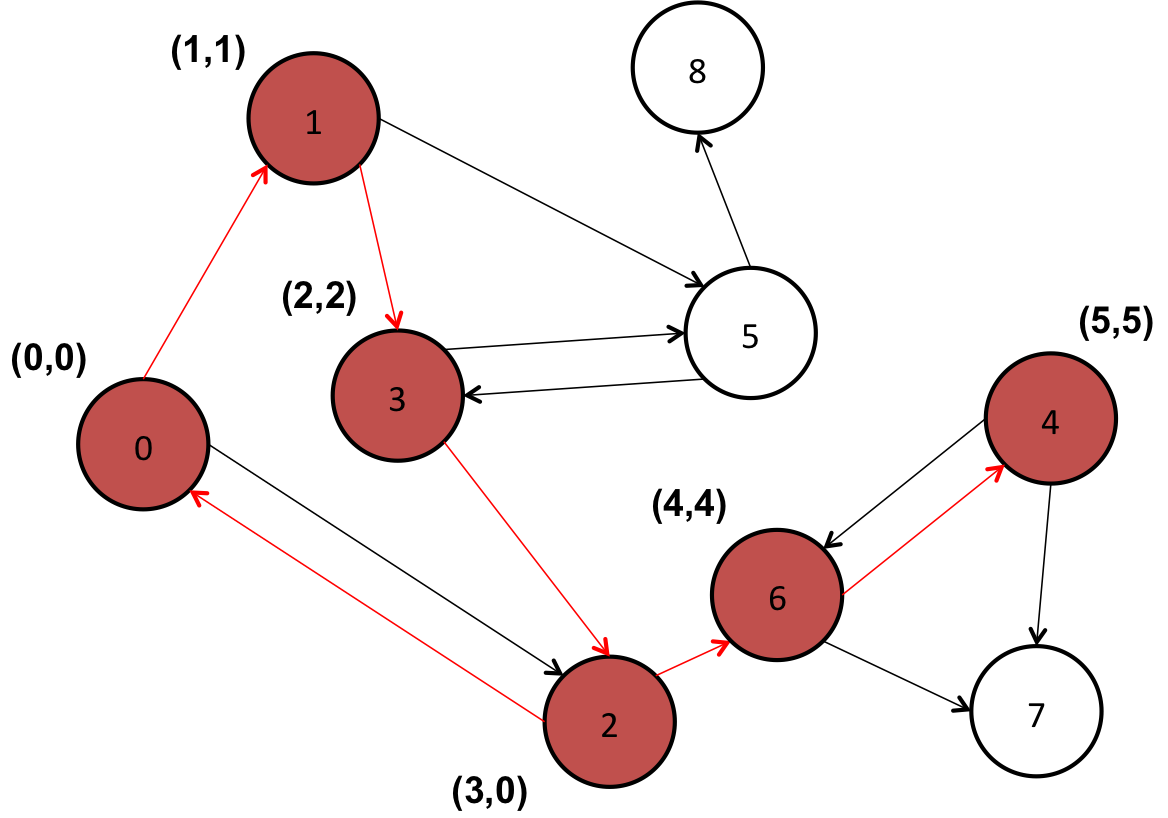
\includegraphics[scale=0.25]{images/tarjan_7.png} }\label{fig:tarjan_1_g}} \qquad
    \subfloat[\tiny{$L = \{ 0,1,3,2,6,4\}$. $low_4 = 4$ because is connected to a node with a smaller index.}]{{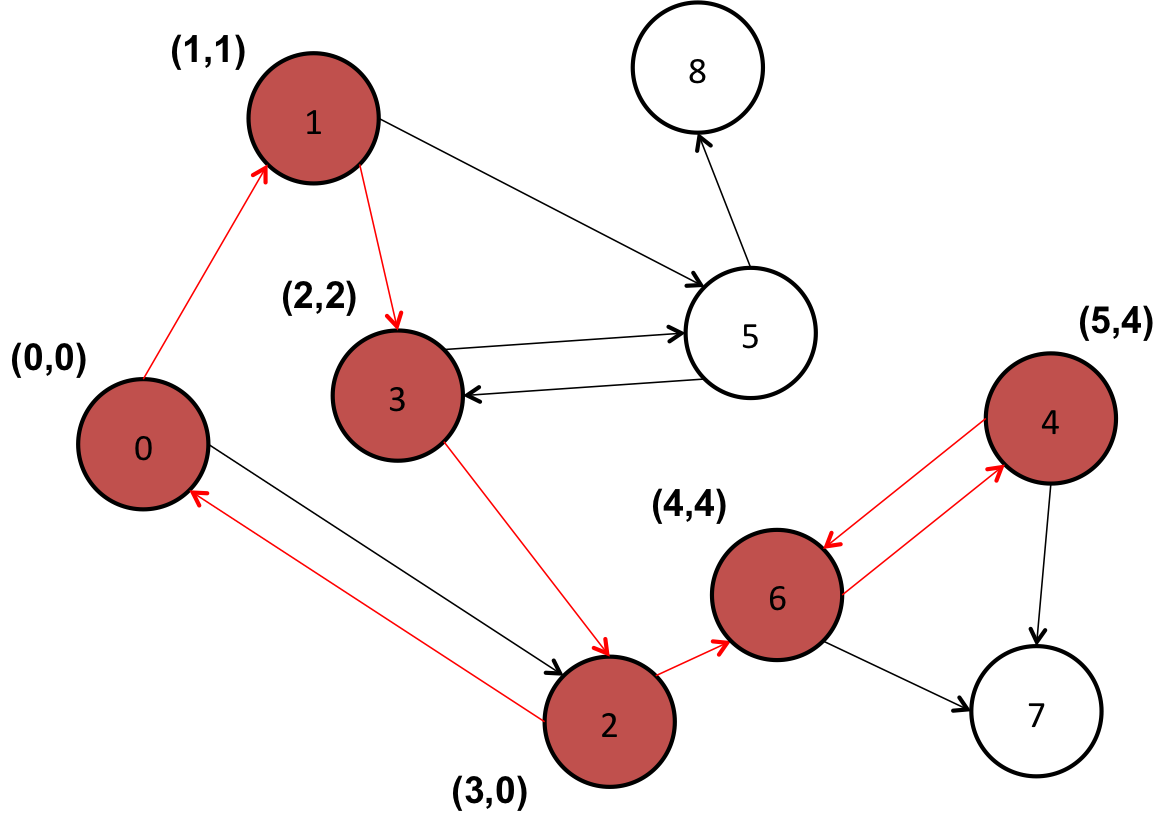
\includegraphics[scale=0.25]{images/tarjan_8.png} }\label{fig:tarjan_1_h}} \\
\end{figure}
\begin{figure}[H]
    \centering
    \subfloat[\tiny{$L = \{ 0,1,3,2,6,4,7\}$. Visit node $7$. Because node $7$ has been full explored and $S_7 = low_7$ then node $7$ is a SCC.}]{{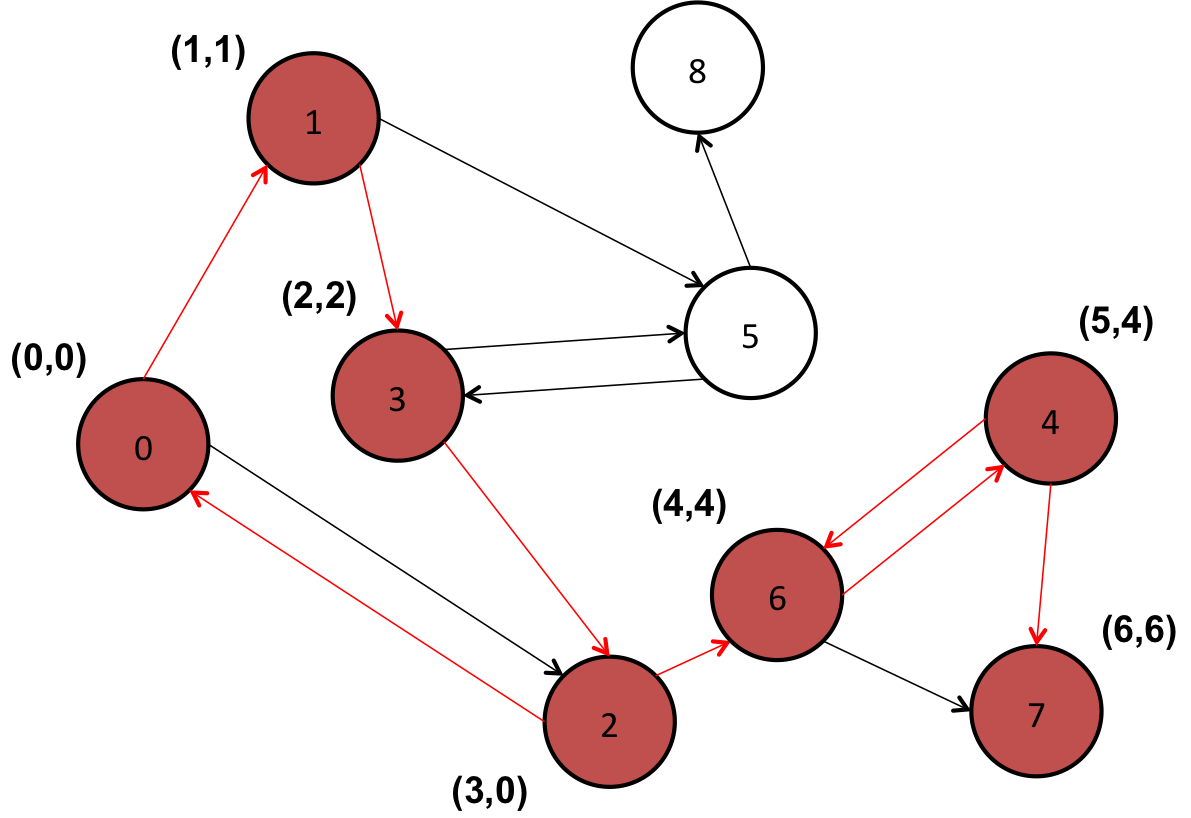
\includegraphics[scale=0.25]{images/tarjan_9.png} }\label{fig:tarjan_2_a}} \qquad
    \subfloat[\tiny{$L = \{ 0,1,3,2,6,4\}$. Node $7$ has been removed from $L$, and $low_6$ remains equal because node $7$ has a larger index. $S_6 = low_6$ meaining that nodes $6$ and $4$ are part of a SCC.}]{{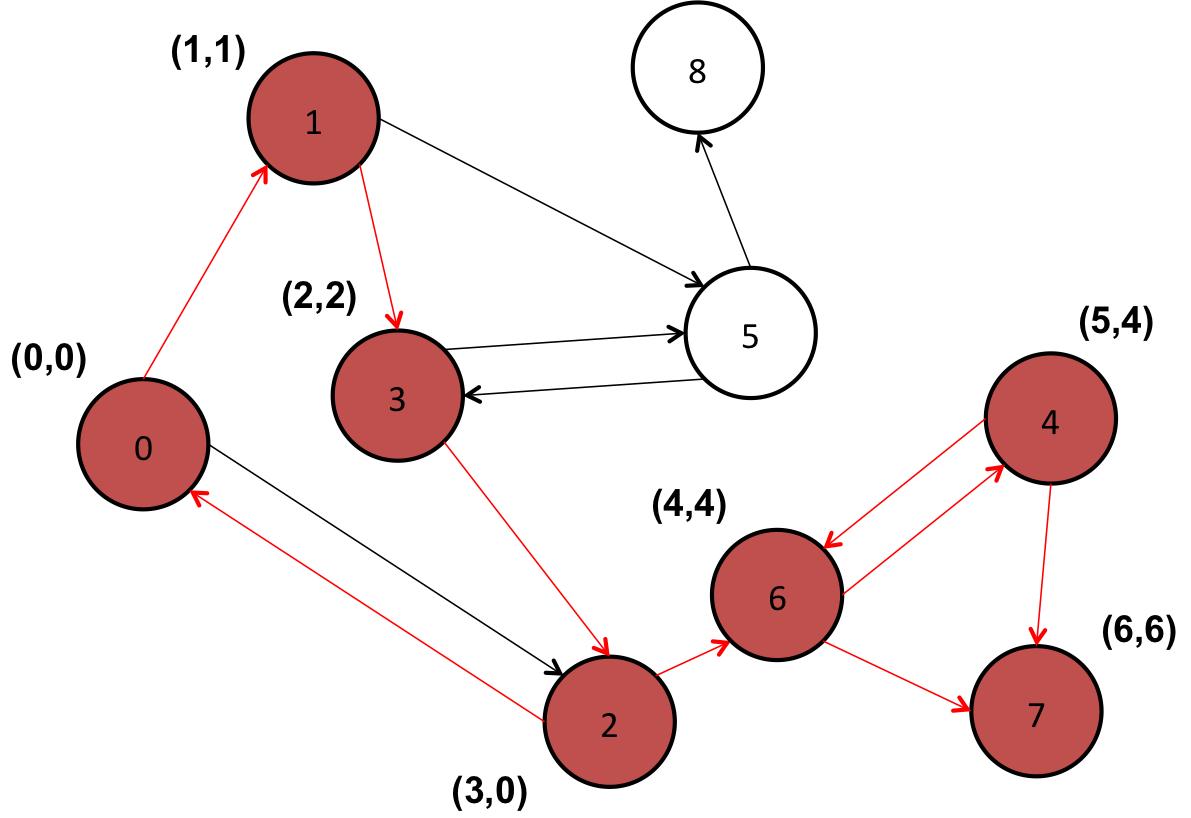
\includegraphics[scale=0.25]{images/tarjan_10.png} }\label{fig:tarjan_2_b}} \\
\end{figure}
\begin{figure}[H]
    \centering
    \subfloat[\tiny{$L = \{ 0,1,3,2\}$. $low_3 = 0$, because it comes from node $2$, and $low_2$ is smaller than $low_3$.}]{{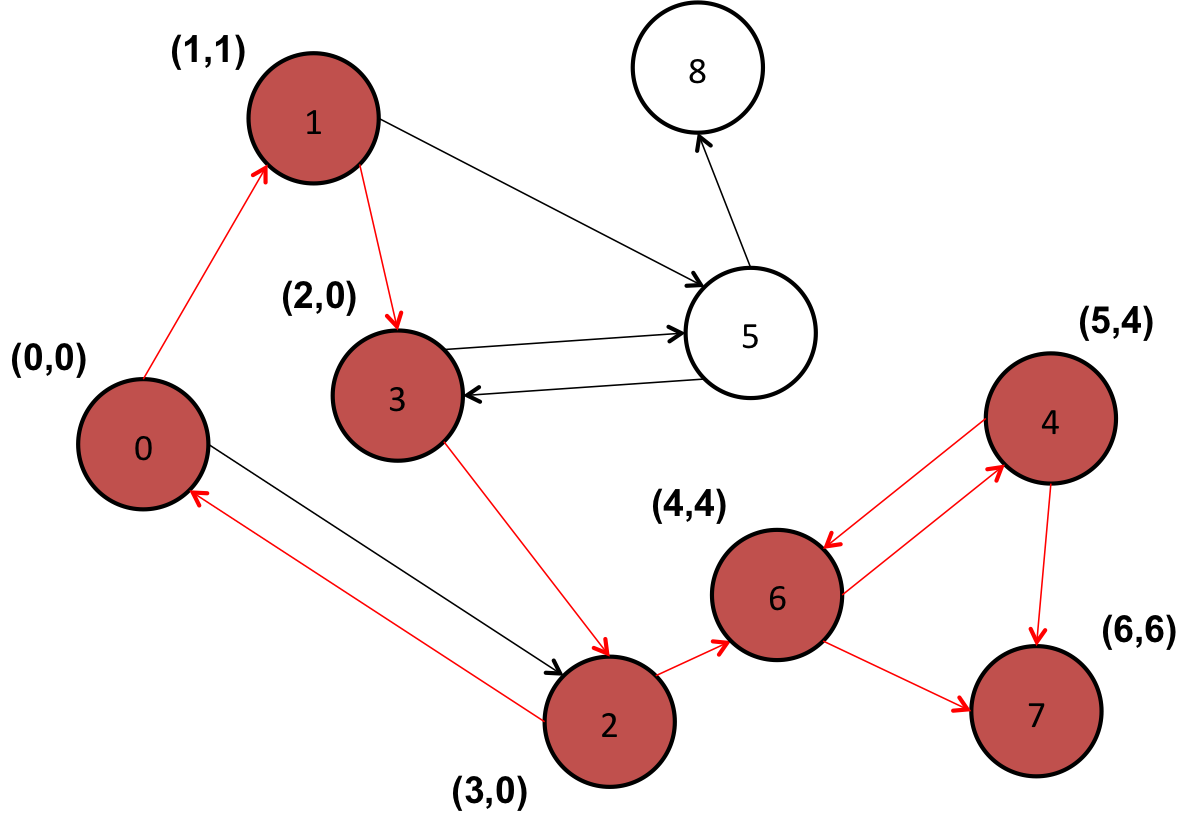
\includegraphics[scale=0.25]{images/tarjan_11.png} }\label{fig:tarjan_2_c}} \qquad
    \subfloat[\tiny{$L = \{ 0,1,3,2,5\}$. Visit node $5$.}]{{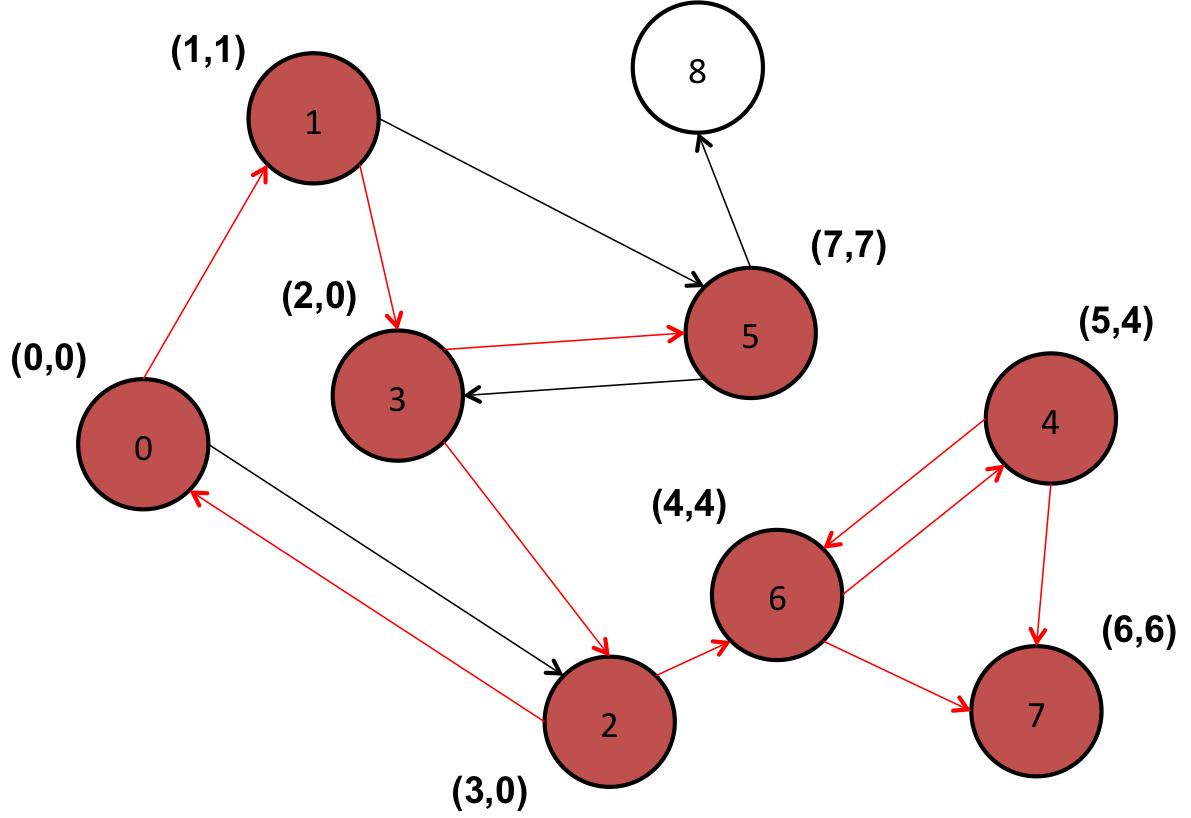
\includegraphics[scale=0.25]{images/tarjan_12.png} }\label{fig:tarjan_2_d}} \\
\end{figure}
\begin{figure}[H]
    \centering
    \subfloat[\tiny{$L = \{ 0,1,3,2,5\}$. $low_5=2$, because is connected to node $3$, which has $S_3=2$.}]{{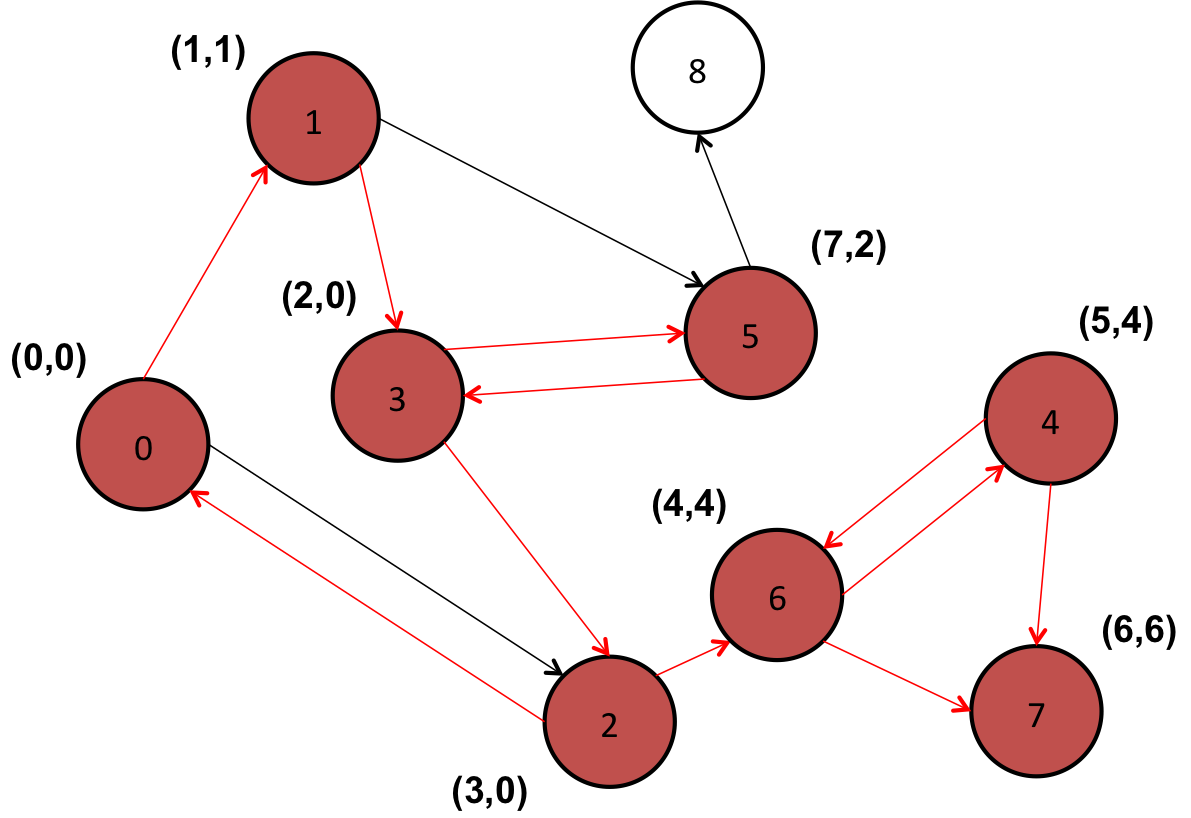
\includegraphics[scale=0.25]{images/tarjan_13.png} }\label{fig:tarjan_2_e}} \qquad
    \subfloat[\tiny{$L = \{ 0,1,3,2,5,8\}$. Visit node $8$. Because node $8$ doesn't have any adjacent nodes and $S_8 = low_8$, it forms another SCC.}]{{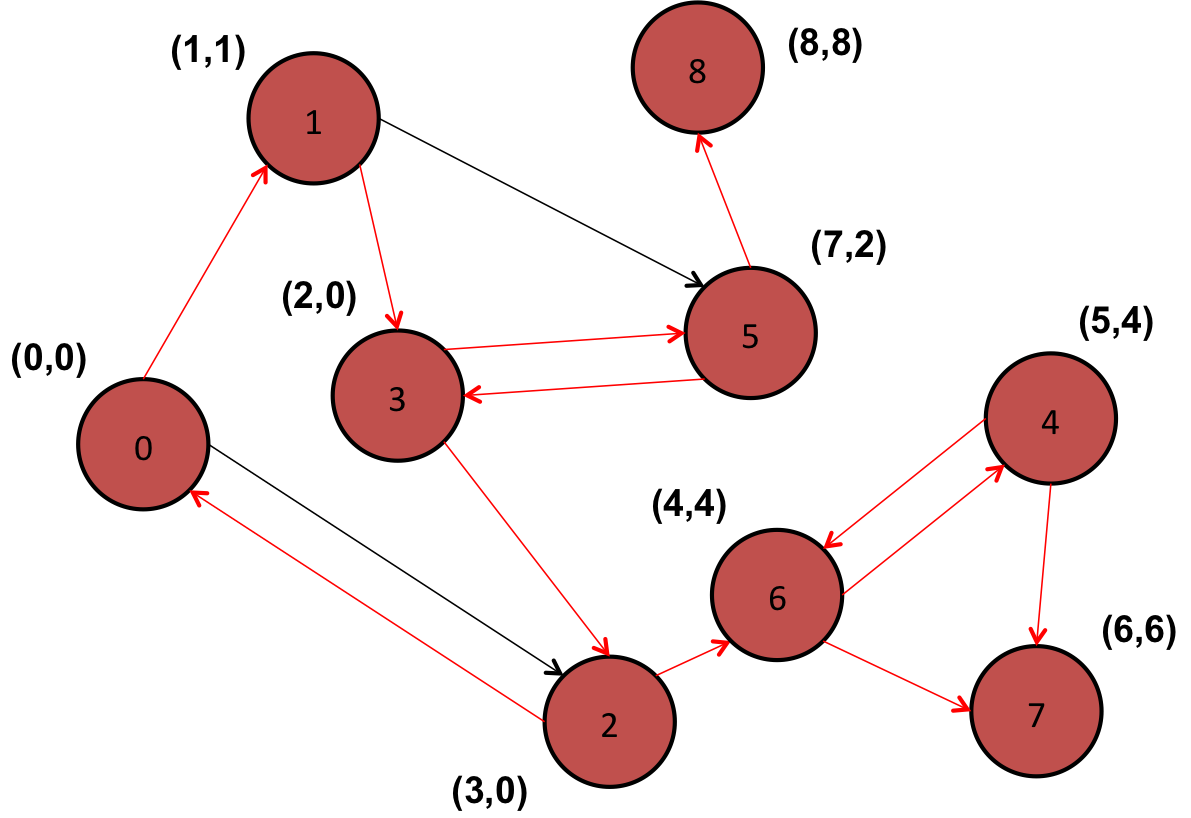
\includegraphics[scale=0.25]{images/tarjan_14.png} }\label{fig:tarjan_2_f}} \\
\end{figure}
\begin{figure}[H]
    \centering
    \subfloat[\tiny{$L = \{ 0,1,3,2,5\}$. $low_1=0$, because it comes from node $3$ and $low_3=0$.}]{{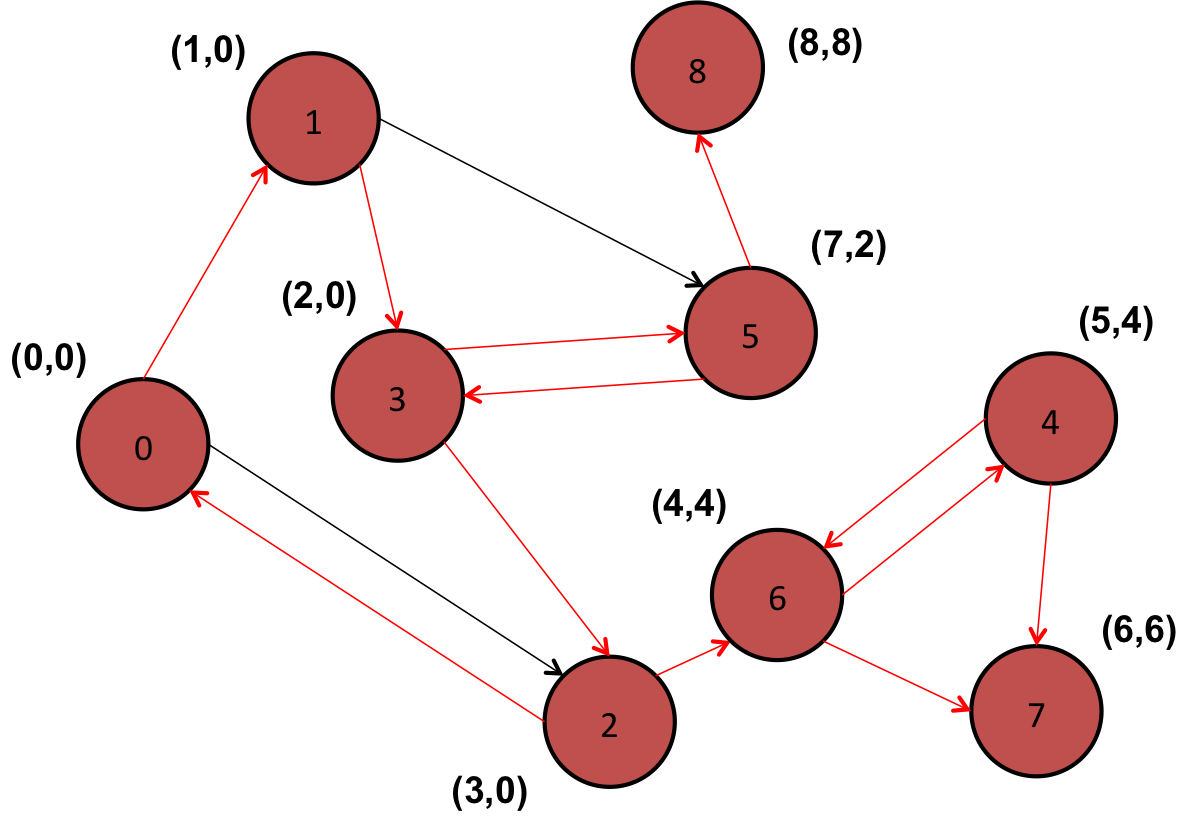
\includegraphics[scale=0.25]{images/tarjan_15.png} }\label{fig:tarjan_2_g}} \qquad
    \subfloat[\tiny{$L = \{ 0,1,3,2,5\}$. $low_1$ remains without change because $S_5$ is larger.}]{{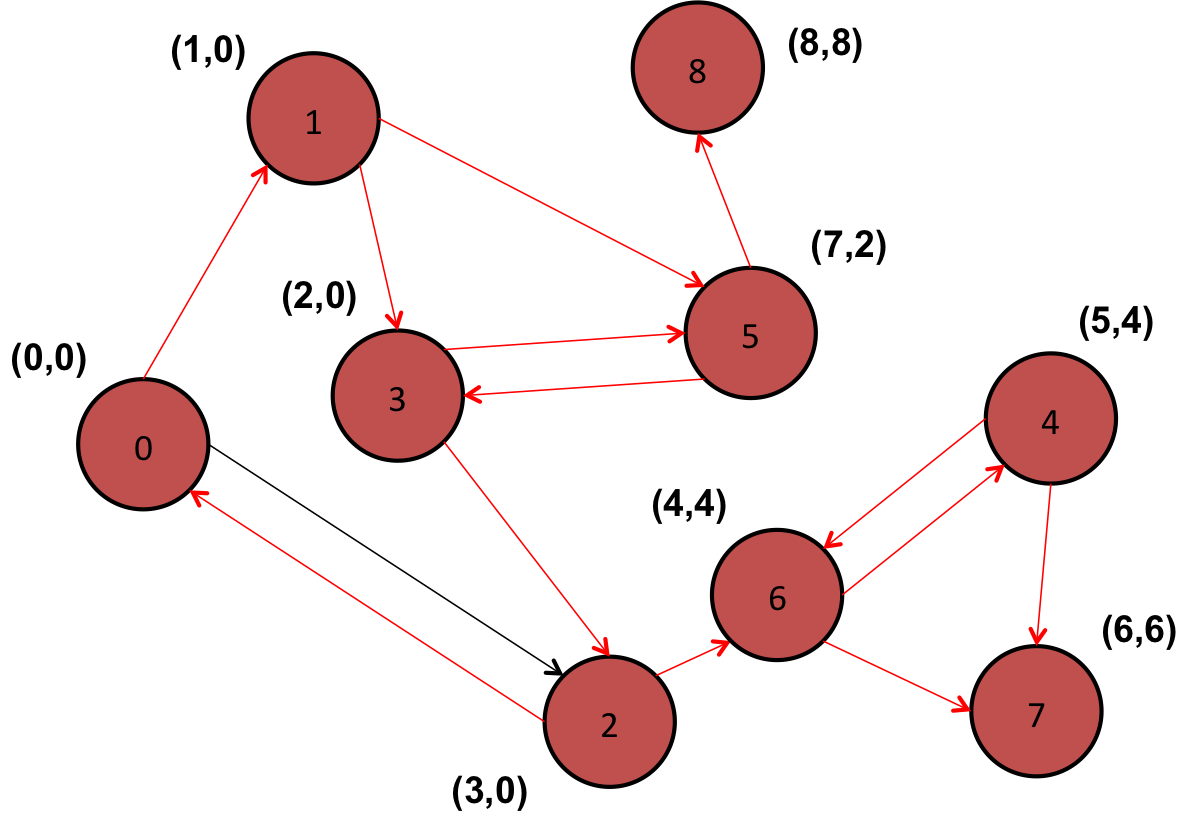
\includegraphics[scale=0.25]{images/tarjan_16.png} }\label{fig:tarjan_2_h}} \\
\end{figure}

\begin{figure}[H]
    \centering
    \subfloat[\tiny{$L = \{ 0,1,3,2,5\}$. $low_0$ remains without change because $S_2$ is larger. $S_0 = low_0$ then nodes $0,1,3,2,5$ are part of a SCC. then all of them are removed from $L$, leaving the stack empty.}]{{\includegraphics[scale=0.25]{images/tarjan_17.png} }\label{fig:tarjan_2_i}} \qquad
    \caption[Tarjan's Algorithm]{Tarjan's algorithm. The values of $S_v$ and $low_v$ are changing in every step of the \textit{DFS} for graph in \ref{fig:scc}. If node $v$, after all its adjacent nodes has been explored, happens that $S_v = low_v$, then $v$ an all nodes inserted to the stack $L$ after $v$ form a SCC.}
    \label{fig:tarjan}
\end{figure}


\subsection{Kosaraju's Algorithm}

\index{Kosaraju's algorithm} In 1983 Aho, Hopcroft, and Ullman \cite{kosaraju} published the algorithm and credit it to S. R. Kosaraju. The algorithm first runs a \textit{DFS} to get a topological sort. The second step is to compute the  transponse of the adjacency matrix. Finally, following the order obtained in the first DFS and using the transponse matrix, the graph is traversed and the number of times a \textit{DFS} is started is the number of SCC's in the graph, and the nodes visited in the same \textit{DFS} are part of the the same SCC.\\

Running a \textit{DFS} using the order obtained in a topological sort will cause to traverse the graph from root nodes to leaf nodes. But using the reversed graph (with the transponse matrix), will cause to traverse the graph from leaf nodes to root nodes.\\

If node $b$ is reachable from node $a$ in the original graph, then $a$ will be reachable from node $b$ in the reversed graph.

\begin{figure}[H]
    \centering
    \subfloat{{\includegraphics[scale=0.25]{images/scc_1.png} }\label{fig:kosaraju_a}} \qquad
    \subfloat{{\includegraphics[scale=0.25]{images/scc_reversed.png} }\label{fig:kosaraju_b}} \\
    \caption[Kosaraju's Algorithm]{\ref{fig:kosaraju_a} shows the original graph. \ref{fig:kosaraju_b} shows the reversed graph with the arrows to point in the opossite direction.}
    \label{fig:kosaraju}
\end{figure}

For the graph in \ref{fig:kosaraju_a} the topological sort would be $0,1,3,5,8,2,6,4,7$, and if we go through that order and start a \textit{DFS} for each node that has not been visited using the reversed graph represented in \ref{fig:kosaraju_b}. We obtain that the first \textit{DFS} visits the nodes $0,2,3,1,5$, and occurs that they form a SCC in the original graph. Following the topological order, the next \textit{DFS} only visits node $8$, the next one visits nodes $6$ and $4$, and the last one visits node $7$. All of them SCC's in the original graph.\\

Compared to Tarjan's algorithm, Kosaraju's algorithm has worst performance, because it need two \textit{DFS}, meanwhile Tarjan only needs one, but on the other hand, Kosaraju doesn't need to store additional information beside the topological sort. Program \ref{lst:kosaraju} implements the Kosaraju's algorithm to identify the number of \textit{SCC's} in a graph $G$.\\

\noindent \textbf{Time Complexity:} $O(n^2)$\\
\textbf{Input:}\\
\indent \texttt{n}. Number of vertices.\\
\indent \texttt{G}. The adjacency matrix.\\
\textbf{Output:}\\
\indent \texttt{L}. Represents the topological sort.\\
\indent \texttt{nComponents}. Stores the number of SCC's

\begin{lstlisting}[caption={Kosaraju's Algorithm}, label={lst:kosaraju}, numbers=left]
void Kosaraju()
{
    int i, j, k, temp;
    
    memset(S,0,sizeof(S));
    nVertex = n-1;
    nComponents = 1;
    
    for(i=0; i<n; i++)              //Apply the first DFS
        if(S[i] == 0)
            DFS(i,true);            //Obtain the post-order traversal
    
    for(i=0; i<n; i++)              //Obtain the transponse of the adjacency matrix
    {
        for(j=i; j<n; j++)
        {
            temp = G[i][j];
            G[i][j] = G[j][i];
            G[j][i] = temp;
        }
    }
    
    memset(S,0,sizeof(S));
    nComponents = 0;
    
    for(i=0; i<n; i++)
    {
        k = L[i];                   //Visit the nodes using the order obtained in
        if(S[k] == 0)               //the first DFS
        {
            nComponents++;          //Increment the number of SCC
            DFS(k,false);
        }
    }
}

void DFS(int v, bool flag)
{
    //Label the vertex with the number
    //of the strongly connected component
    //it belongs.

    S[v] = nComponents;
    
    for(int i=0; i<n; i++)
        if(G[v][i] == 1 && S[i] == 0)
            DFS(i,flag);
    
    if(flag)                        //if flag is true
        L[nVertex--] = v;           //Add v to the stack
}
\end{lstlisting}


\subsection *{Articulation Points}

\index{articulation point} An articulation point in a graph is a vertex that if removed, the graph becomes disconnected. See figure \ref{fig:articulation_points}.\\ 

A variant of Tarjan's algorithm can be used to find articulation points. Basically a node $v$ is an articulation point if:

\begin{enumerate}
    \item $v$ is the root and has more than one children.
    \item if $low_i \geq S_v$, where $i$ is the adjacent node of $v$ which the recursive function of the \textit{DFS}  returns from. This means that there is no connection from node $i$ to previously indexed nodes, so removing $v$ will disconnect the graph.
\end{enumerate}

\begin{figure}[H]
	\centering
	\includegraphics[scale = 0.4]{images/articulation.png}
	\caption[Articulation Points]{Nodes $2$ and $3$ are articulation points, because if they are removed the graph becomes disconnected. Node $1$ is not an articulation point, because node $0$ is directed connected to node $2$.}
	\label{fig:articulation_points}
\end{figure}

The code \ref{lst:articulation} increments the variable \texttt{nLinks} in one every time an articulation point is found. The vector $V$ is used to avoid counting duplicated articulation points.\\ 

\begin{lstlisting}[caption={Articulation Points}, label={lst:articulation}, numbers=left]
void DFS(int v, int prev)
{
    S[v] = nVertex++;
    low[v] = S[v];
    
    for(int i=0; i<n; i++)
    {
        if(graph[v][i] == 1)
        {
            if(x[i] == -1)  //if it's a tree vertex (unvisited)
            {
                DFS(i,v);
                low[v] = min(low[v],low[i]);
                
                if(S[v] == 0)
                {
                    if(S[i] >= 2 && V[v] == 0)
                    {
                        V[v] = 1;
                        nLinks++; //is an articulation point
                    }
                }
                else if(low[i] >= S[v] && V[v] == 0)
                {
                    V[v] = 1;
                    nLinks++;   //is an articulation point
                }
            }
            else if(i != prev)
                low[v] = min(low[v],S[i]);
        }
    }
}
\end{lstlisting}

\subsection *{Bridge Detection}

\index{bridge} A bridge is an edge that if removed the graph becomes disconnected. See figure \ref{fig:bridges}. As with the articulation points, a variant of Tarjan's algorithm can be used to find bridges. For this case we say there is a bridge connecting nodes $i$ and $v$ if $low_i > S_v$, where $i$ is the node which the recursive function returns from. That means that node $i$ cannot reach any of the nodes indexed before him, so if we remove the edge $v - i$, node $i$ will not be able to reach any of the previously indexed nodes.

\begin{figure}[H]
	\centering
	\includegraphics[scale = 0.4]{images/bridges.png}
	\caption[Bridges]{The edge connecting nodes $2$ and $3$, and the edge connecting nodes $3$ and $4$ are bridges. None of the other edges if removed disconnects the graph.}
	\label{fig:bridges}
\end{figure}

The program \ref{lst:bridges} increments by one the variable \texttt{nBridges} when a bridge is found given a graph $G$.\\

\begin{lstlisting}[caption={Bridge Detection}, label={lst:bridges}, numbers=left]
void DFS(int v, int prev)
{
    S[v] = nVertex++;
    low[v] = S[v];
    
    for(int i=0; i<n; i++)
    {
        if(G[v][i] == 1)
        {
            if(S[i] == -1)
            {
                DFS(i,v);
                
                if(low[i] > S[v])   //There is a bridge between i and v
                    nBridges++;
                low[v] = min(low[v],low[i]);
            }
            else if(i != prev)  //Is a back edge
                low[v] = min(low[v],S[i]);
        }
    }
}
\end{lstlisting}

\section{Minimum Spanning Tree}

\index{MST. minimmum spanning tree} Consider a weighted graph with $n$ nodes and $m$ edges that is connected and is not directed. The minimum spanning tree (MST) of that graph is a sub-graph with the following characteristics.

\begin{enumerate}
    \item Contains $n-1$ edges
    \item The graph remains connected
    \item the cost of the tree is minimum
\end{enumerate}

The points listed above describe a sub-graph with no cycles, where all the nodes are connected, and which cost is minimal. The cost of a MST is the sum of the weights of all its edges. Image \ref{fig:mst} shows an example of a MST in a graph. Is important to notice that a graph can have more than one MST. 

\begin{figure}[H]
    \centering
    \subfloat[Connected graph]{{\includegraphics[scale=0.25]{images/mst1.png} }\label{fig:mst1}}
    \qquad
\end{figure}
\begin{figure}[H]
    \centering
    \subfloat[MST of the graph]{{\includegraphics[scale=0.25]{images/mst2.png} }\label{fig:mst2}}
    \caption[Minimum Spanning Tree]{Image \ref{fig:mst1} shows a connected and not directed graph. Image \ref{fig:mst2} shows in red solid lines the $n-1$ edges that are part of the MST wit a cost of 21.}
    \label{fig:mst}
\end{figure}

In this section we will analyze two algorithms that allow us to find the \textit{MST}. One is the \textit{Kruskal's algorithm} and the other is the \textit{Prim algorithm}. Each one have its own advantages and for some problems is better to use one over the other, but at the end the problem is the same, to find a set of edges that are part of the $MST$.

\subsection {Kruskal's Algorithm}

\index{Kruskal's algorithm} Reported by Joseph Kruskal in 1956 \cite{kruskal}. Kruskal's algorithm first needs to sort the edges in the graph in ascending order according to their weights. Then iterate from the beginning of the sorted array of edges and check if the current edge creates a cycle, if it does, discard it and move to the next edge, otherwise add that edge to the MST.\\

One way to check if an edge creates a cycle is to use the Union-Find algorithm, just take the nodes connected by the edge and if those nodes are part of the same set then that edge will create a cycle. If they are part of different sets, then the edge will not create a cycle, so add it to the MST and merge both sets. Figure \ref{fig:kruskal} shows how Kruskal's algorithm works to find the MST of the graph in \ref{fig:mst1}.\\

\begin{figure}[H]
    \centering
    \subfloat[The edge with minimum cost is the one connecting nodes 2 and 3, add it to the MST.]{{\includegraphics[scale=0.3]{images/kruskal_1.png} }\label{fig:kruskal_1}}
    \qquad
    \subfloat[The next edge is $ 2-4$, it doesn't form a cycle so is added to the MST.]{{\includegraphics[scale=0.3]{images/kruskal_2.png} }\label{fig:kruskal_2}}\\
\end{figure}
\begin{figure}[H]
    \centering
    \subfloat[The next edge is $2-5$ and is added to the MST.]{{\includegraphics[scale=0.3]{images/kruskal_3.png} }\label{fig:kruskal_3}}
    \qquad
    \subfloat[The next edge is the one connecting  nodes $3$ and $4$, but if it is added it will create a cycle, so we skip this edge. ]{{\includegraphics[scale=0.3]{images/kruskal_4.png} }\label{fig:kruskal_4}}\\
\end{figure}
\begin{figure}[H]
\centering
    \subfloat[Add edge $0 - 1$ to the MST.]{{\includegraphics[scale=0.3]{images/kruskal_5.png} }\label{fig:kruskal_5}}
    \qquad
    \subfloat[The edge $1-3$ is added to the MST. We have added all 5 edges, any other edge will generate a cycle, so we can stop looking.]{{\includegraphics[scale=0.3]{images/kruskal_6.png} }\label{fig:kruskal_6}}\\
    \caption[Kruskal's Algorithm]{Kruskal's algorithm needs that the edges to be previously sorted by their cost. Once $n-1$ edges are added to the MST the process can be stopped.}
    \label{fig:kruskal}
\end{figure}

The performance of Kruskal's algorithm will depend on the algorithm used to sort the edges, and the algorithm used to identify cycles. For the sorting part an algorithm that runs in $O(m \log m)$ can be used, like \textit{Merge Sort} and \textit{Heap Sort}. To detect cycles is recommended to use the \textit{Union-Find} algorithm, which runs in $O(\log n)$ and is easy to implement.\\

The code showed in \ref{lst:kruskal} implements a class \texttt{Edge} to easily represent an edge and be able to create an array of edges. This class contains three values $u,v$ and $w$ indicating that there is an edge connecting nodes $u$ and $v$ with a cost of $w$. The overloaded operator is needed to sort the edge array. The program uses the \textit{Union-Find} method described in \ref{lst:union_find}.\\

\noindent \textbf{Time Complexity:} $O(m \log m + m \log n)$\\
    \indent $O(m \log m)$ to sort all the edges\\
    \indent $O(m \log n)$ for the union find of the sorted edges\\
\textbf{Input:}\\
\indent $edge$. A vector with all the edges in the graph.\\
\textbf{Output:}\\
\indent The cost of the MST.

\begin{lstlisting}[caption={Kruskal's Algorithm}, label={lst:kruskal}, numbers=left]
#include <vector>
#include <algorithm>

using namespace std;

class Edge
{
public:
    int u;
    int v;
    int w;
    
    Edge(int u = 0, int v = 0, int w = 0)
    {
        this->u = u;
        this->v = v;
        this->w = w;
    }
    
    bool operator < (const Edge &b) const
    {
        return this->w < b.w;
    }
};

vector<Edge> edge;
int nVertex;

int Kruskal()
{
    int i, n;
    int a, b, w;
    int d = 0;
    
    sort(edge.begin(), edge.end());
    
    n = nVertex;
    for(i=0; n>1; i++)
    {
        a = edge[i].u;
        b = edge[i].v;
        w = edge[i].w;
        
        if(find_set(a) != find_set(b))
        {
            d += w;
            union_set(a,b);
            n--;
        }
    }
    
    return d;
}
\end{lstlisting}

\subsection {Prim's Algorithm}

\index{Prim's algorithm} Discovered by Prim \cite{prim}, but invented earlier by V. Jarník in 1930. Prim's algorithm is very similar to Dijkstra's algorithm. The adjacency matrix is filled with $\infty$ in those locations where there is no edge. The initial node doesn't matter in Prim, any node can be used as the  initial node. In every iteration as in Dijkstra's the minimum value of vector $D$ must found across all non-visited nodes, and then proceed to update the vector $D$. While in Dijkstra's the vector $D$ is updated with the cost to move from the initial node to other non-visited nodes, in Prim the vector is updated using only the weight of the edges. The value of element $D_J$ is given by the equation \ref{eq:prim}.

\begin{equation}
    D_j = \min \left ( D_j, W_{kj} \right ), 
\label{eq:prim}
\end{equation}

where $k$ represents the position of the minimum value of $D$ across the non-visited vertices. Table \ref{table:prim} shows the vector $D$ in every iteration of Prim algorithm for the graph in \ref{fig:mst1} and node $0$ as the initial node.\\

\begin{table}[H]
\centering % used for centering table
\begin{tabular}{c | c | c | c | c | c | c |}
\hline
\textit{it. 1} & $\textcolor{red}{0}$ & $\infty$ & $\infty$ & $\infty$ & $\infty$ & $\infty$\\
\hline
\textit{it. 2} & $\textbf{0}$ & $\textcolor{red}{6}$ & $\infty$ & $10$ & $\infty$ & $\infty$\\
\hline
\textit{it. 3} & $\textbf{0}$ & $\textbf{6}$ & $10$ & $\textcolor{red}{7}$ & $9$ & $\infty$\\
\hline
\textit{it. 4} & $\textbf{0}$ & $\textbf{6}$ & $\textcolor{red}{1}$ & $\textbf{7}$ & $5$ & $\infty$\\
\hline
\textit{it. 5} & $\textbf{0}$ & $\textbf{6}$ & $\textbf{1}$ & $\textbf{7}$ & $\textcolor{red}{3}$ & $4$\\
\hline
\textit{it. 6} & $\textbf{0}$ & $\textbf{6}$ & $\textbf{1}$ & $\textbf{7}$ & $\textbf{3}$ & $\textcolor{red}{4}$\\
\hline
\end{tabular}
\caption[Prim's Algorithm]{Vector $D$ for the Prim algorithm. Red numbers represents the minimum value chosen in an specific iteration. Bold numbers represent already visited nodes.}
\label{table:prim}
\end{table}

The cost of the MST for the graph \ref{fig:mst1} is the sum of all red numbers in table \ref{table:prim}, $0+6+7+1+3+4=21$. If we want to know which edges are part of the MST, then we must have a record of the nodes connected to the ones represented in $D$, something similar to how a path is obtained in \textit{Dijkstra}. The program \ref{lst:prim} consists on a function \texttt{Prim} that returns the cost of the \textit{MST} of a graph given its weighted matrix $W$ by using the \textit{Prim} algorithm starting from node $0$.\\

\noindent \textbf{Time Complexity:} $O(n^2)$\\
\textbf{Input:}\\
\indent $n$. AThe number of nodes. \\
\indent $W$. A weighted and connected graph. \\
\textbf{Output:}\\
\indent The cost of the MST.

\begin{lstlisting}[caption={Prim Algorithm}, label={lst:prim}, numbers=left]
int Prim()
{
    int i, j, k, minVal;
    int d = 0;
    
    for(i=1; i<n; i++)
    {
        D[i] = W[0][i];
        V[i] = 0;
    }
    
    V[0] = 1;
    
    for(i=1; i<n; i++)
    {
        minVal = oo;
        k = -1;
        
        for(j=1; j<n; j++)
        {
            if(V[j] == 0 && D[j] < minVal)
            {
                minVal = D[j];
                k = j;
            }
        }
        
        if(k == -1)
        {
            printf("Error: No connection found");
            break;
        }
        
        d += D[k];
        
        V[k] = 1;
        for(j=1; j<n; j++)
            if(V[j] == 0 && W[k][j] < D[j])
                D[j] = W[k][j];
    }
    
    return d;
}
\end{lstlisting}

\section{Maximum Bipartite Matching}

\index{bipartite graph}  A bipartite graph can be defined as a two sets of vertices $A$, and $B$, where all the edges connect a node from set $A$ with a node of set $B$. Elements of the same set are not connected directly.\\

\index{matching} A matching is a set of edges, where no two edges share a common vertex. \index{maximum bipartite matching} Then a maximum matching is a matching that contains the largest number of edges.\\

Consider the case of an university that has $n$ professors labeled as $0, 1, \cdots n-1$, and $m$ courses numbered as $0, 1 \cdots, m-1$. By politics of the university, no professor can teach more than one course, if a professor cannot be found to teach a course, then that course cannot be opened that semester. The goal is to maximize the number of courses that can be imparted in the semester.\\

This taks can be seen as a graph, where courses and professors are the nodes, and an edge from node $i$ to node $j$ means that professor $i$ can teach course $j$. See image \ref{fig:maximummatching}.

\begin{figure}[H]
	\centering
	\includegraphics[scale = 0.3]{images/bipartite1.png}
	\caption[Bipartite Graphs]{Bipartite graph with four professors and three courses.}
	\label{fig:maximummatching}
\end{figure}

For the bipartite graph in \ref{fig:maximummatching}, one possible solution is that professor 0 teach course 1, professor 1 teach course 2, and professor 2 teach course 0, with that arrangement all the courses can be opened for the semester. Professor 3 can have a sabatical year.\\

One possible solution for this problem is to try to assign a professor $p$ to some course $c$ that doesn't has a professor assigned, or if it already has a professor assigned, then try move the current professor to another course, in order that professor $p$ teaches course $c$. That idea is basically a \textit{DFS}, which have a time complexity of $O(V + E)$, for this case $V = n + m$, and $E \leq n*m$. The search is repeated $m$ times, meaning that that the time complexity for the algorithm is $O(mn + m^2 + nm^2) = O(nm^2)$. The implementation for this solution is showed in program \ref{lst:bipartite_matching}.\\ 

\noindent \textbf{Time Complexity:} $O(nm^2)$\\
\textbf{Input:}\\
\indent \textit{n}. Number of professors. $1 \leq n \leq 100$.\\
\indent \textit{m}. Number of courses. $1 \leq m \leq 100$.\\
\indent \textit{graph}. The bipartite graph, where $graph_{ij} = true$ if professor $i$ can teach course $j$.\\
\textbf{Output:}\\
\indent \textit{cnt}. The maximum matching.

\begin{lstlisting}[caption={Maximum Bipartite Matching}, label={lst:bipartite_matching}, numbers=left]
#include <cstring>
#define M 128
#define N 128

bool graph[M][N];
bool seen[N];
int matchL[M], matchR[N];
int n, m;
bool bpm(int);

int main()
{
    // Read input and populate graph[][] // Set m, n
    memset(matchL, -1, sizeof(matchL));
    memset(matchR, -1, sizeof(matchR));
    
    int cnt = 0;
    for(int i=0; i<m; i++)
    {
        memset(seen, 0, sizeof(seen)); 
        if(bpm(i))
            cnt++;
    }
    // cnt contains the number of happy pigeons
    // matchL[i] contains the hole of pigeon i or -1 if pigeon i is unhappy 
    // matchR[j] contains the pigeon in hole j or -1 if hole j is empty
    
    return 0;
}

bool bpm(int u)
{
    for(int v=0; v<n; v++)
    {
        if(graph[u][v])
        {
            if(seen[v])
                continue;
            
            seen[v] = true;
            
            if(matchR[v] < 0 || bpm(matchR[v]))
            {
                matchL[u] = v;
                matchR[v] = u;
                return true;
            }
        }
    }
    return false;
}
\end{lstlisting}

\section{Flow Network}

\index{flow network}  A flow network is a directed graph where each edge has a capacity and each edge receives a flow. The amount of flow on an edge cannot exceed the capacity of the edge. A flow must satisfy that the amount of flow into a node equals the amount of flow out of it, unless it is a source, which has only outgoing flow, or sink, which has only incoming flow.\\

A network is a graph $G = (V,E)$, together with a non-negative function $c: V \times V \to \Re$, called the capacity function, and a flow function $f: V \times V \to \Re$, such that:

\begin{itemize}
\item Incoming flow is equal to outgoing flow. $f(u,v) = -f(v,u)$.
\item The flow through an edge cannot exceed its capacity. $f(u,v) \leq c(u,v)$.
\end{itemize}

Network flow can be uses to model fluid in pipes, traffic systems, image denoising, electrical current, among others applications.

\subsection{Ford-Fulkerson Algorithm}

\index{Ford-Fulkerson algorithm} Invented in 1956 by L. R. Ford, and D. R. Fulkerson \cite{ford_fulkerson}. Ford-Fulkerson's algorithm finds the maximum flow in a network. In order to achieve this, a path, $s_1, s_2, \cdots, s_k$, between source and sink must be found, where $s_1$ is the source, and $s_k$ is the sink. \index{augmenting path} This path is called \textit{augmenting path}. An edge $(u,v)$ can be used in the augmenting path only if:

\begin{equation}
c(u,v) - f(u,v) > 0 
\label{eq:ford-fulkerson1}
\end{equation}

If not augmenting path is found the algorithm ends, otherwise, the maximum amount of flow $(f_{max})$ that can travel trough this path must be calculated using equation \ref{eq:ford-fulkerson1} for each edge of the augmenting path and add that value to the network flow.

\begin{align}
f(s_i,s_{i+1}) &= f(s_i,s_{i+1}) + f_{max}\\
f(s_{i+1},s_i) &= f(s_{i+1},s_i) - f_{max}
\label{eq:ford-fulkerson2}
\end{align}

for every $i=1,2, \cdots, k-1$.\\

Once this is done, another augmenting path must be found, and the process is repeated until no augmenting path is found.\\

The execution time for this algorithm depends in the algorithm used to find the augmenting path. The code bellow uses a \textit{BFS} to do that, which has a time complexity of $O(V + E)$, and in the worst case for every augmented path founded the flow will increase in 1 unit, meaning that the time complexity of \textit{Ford-Fulkerson} is $O(F(V+E))$, where $F$ is the maximum flow of the network.\\

The \texttt{Max\_Flow} function in \ref{lst:max_flow} receives the \textit{source} and \textit{sink} of the network, and by using matrix $w$ as the capacity function, and matrix $flow$ as the flow function, it returns the maximum flow by using the \textit{Ford-Fulkerson} algorithm.\\

\noindent \textbf{Time Complexity:} $O(f(m+n))$\\
\indent \textit{f}. Maximum flow\\
\textbf{Input:}\\
\indent \textit{n}. Number of nodes. $2 \leq n \leq 100$\\
\indent \textit{w}. Capacity function\\
\indent \textit{source}. Source node\\
\indent \textit{sink}. Sink node\\
\textbf{Output:}\\
\indent The maximum flow

\begin{lstlisting}[caption={Ford-Fulkerson Algorithm}, label={lst:max_flow}, numbers=left]
#include <cstring>
#include <algorithm>
#include <queue>

using namespace std;

#define N 105
#define WHITE 0
#define GRAY 1
#define BLACK 2
#define oo 100000000

long w[N][N];       //Adjacency matrix
long flow[N][N];    //Flow matrix
long color[N], pred[N];
long n;
queue<long> Q;

long Max_Flow (long source, long sink)
{
    long i, j, u;
    long increment;
    
    // Initialize empty flow.
    long max_flow = 0;
    memset(flow,0,sizeof(flow));
    
    // While there exists an augmenting path,
    // increment the flow along this path.
    while (BFS(source,sink))
    {
        // Determine the amount by which we can increment the flow.
        increment = oo;
        
        for (u=sink; pred[u]>=0; u=pred[u])
            increment = min(increment,w[pred[u]][u]-flow[pred[u]][u]); // Now increment the flow.
        
        for (u=sink; pred[u]>=0; u=pred[u])
        {
            flow[pred[u]][u] += increment;
            flow[u][pred[u]] -= increment;
        }
        
        max_flow += increment;
    }
    
    // No augmenting path anymore. We are done.
    return max_flow;
}
\end{lstlisting}

The task of the \texttt{BFS} \index{BFS. breadth first search} function is to find the augmenting path across the network. It receives the indexes of the source and sink nodes, and stores the augmenting path in the array \texttt{pred}. If the sink cannot be reached it returns \texttt{false}, otherwise returns \texttt{true}.

\begin{lstlisting}[numbers=left]
long BFS (long start, long target)
{
    long u,v;
    
    memset(color,0,sizeof(color));

    Q.push(start);
    pred[start] = -1;
    color[start] = GRAY;
    
    while (!Q.empty())
    {
        u = Q.front();
        
        color[u] = BLACK;
        
        // Search all adjacent white nodes v. If the capacity
        // from u to v in the residual network is positive,
        // enqueue v.
        
        for (v=0; v<n; v++)
        {
            if (color[v]==WHITE && w[u][v]-flow[u][v]>0)
            {
                Q.push(v);
                pred[v] = u;
                color[v] = GRAY;
            }
        }
    }
    
    // If the color of the target node is black now,
    // it means that we reached it.
    
    return color[target]==BLACK;
}
\end{lstlisting}


\section{Some Variants}

Some of the algorithms seen in this chapter can be modified to solve specific kind of problems. In this section we will review some of these problems.\\

\subsection{Minmax and Maxmin}

\index{minmax} \index{maxmin} The algorithms of minmax and maxmin are variants of shortest path algorithms. In minmax, the edge with maximum value is found for each path and returns the minimum of those values. In a similar way, the maxmin algorithm finds the edge with minimum value for all paths and returns the largest among those values. Following there are two examples that illustrates the concepts of minmax and maxmin algorithms.

\subsection *{Example. Credit Card (minmax)}

\index{minmax} For the graph in \ref{fig:minmax} suppose that Johnny wants to travel from city $A$ to city $G$ using his credit card. That credit card has a limit of $K$ dollars, and Johnny can use it as many times he wants as long he doesn't surpass $K$ dollars in a single purchase.\\

\begin{figure}[H]
	\centering
	\includegraphics[scale = 0.4]{images/minmax.png}
	\caption[Minmax]{Toll fares of roads across cities.}
	\label{fig:minmax}
\end{figure}

To get from city $A$ to city $G$ Johnny may follow the following path: $A-C-F-G$. In that case the credit card limit must be at least $140$ dollars. For the paths $A-B-E-G$, $A-B-D-G$ and $A-C-F-D-G$ The credit card's limit must be at least of 90, 120 and 80 dollars respectively. There are other paths, too. However, it is clear that $A-C-F-D-G$ is the one that needs a minimum value of $K$ of $80$ dollars.\\

Given the road connections between cities and the toll fare of each one of the roads, we must find the minimum value of $K$ that is necessary to Johnny to get from a starting city to a destination city. The first line contains three numbers $C$ $(2 \leq C \leq 100)$, $S$ $(1 \leq S \leq 1000)$ and $Q$ $(1 \leq Q \leq 10000)$, indicating the number of cities, roads, and queries respectively. $S$ lines follow, each one with three numbers $a,b$ and $c$, meaning that there is a road connecting city $a$ with city $b$, with a toll fare of $c$ dollars. Finally there are $Q$ lines, each one with two numbers $C_{start}$ and $C_{end}$ indicating the starting city and the destination city for Johnny.\\

For each query we must print the minimum value of $K$ necessary to reach the destination city. In case there is no path just print ''no path''.\\

The solution for this problem is showed in \ref{lst:minmax} and consists on just applying the minmax algorithm. They are asking for the minimum edge weight among the maximum edge weight of all the paths. To accomplish this one option is to apply the Floyd-Warshall algorithm modified.

$$
W_{ij} = \min(W_{ij}, \max(W_{ik},W_{kj}))
$$

The only condition is to initialize the weighted matrix $W$ with $\infty$, except for the main diagonal that will remain with $0$'s.\\

\begin{lstlisting}[caption={Minmax Algorithm}, label={lst:minmax}, numbers=left]

#include <cstdio>
#include <algorithm>
#define MAX 32767

using namespace std;

int w[101][101];

void initialize(int);
void Floyd_Warshall(int);

int main ()
{
    int C, S, Q, i, a, b, d, c1, c2;
    
    scanf("%d %d %d", &C, &S, &Q);
    
    initialize(C);
        
    for(i=0; i<S; i++)
    {
        scanf("%d %d %d", &c1, &c2, &d);
        w[c1][c2] = d;
        w[c2][c1] = d;
    }
        
    Floyd_Warshall(C);
        
    for(i=0; i<Q; i++)
    {
        scanf("%d %d", &a, &b);
        
        if(w[a][b] == MAX)
            printf("no path\n");
        else
            printf("%d\n", w[a][b]);
    }
    
    return 0;
}

void initialize(int n)
{
    int i, j;
    
    for(i=0; i<=n; i++)
    {
        for(j=0; j<=n; j++)
        {
            if(i == j)
                w[i][j] = 0;
            else
                w[i][j] = MAX;
        }
    }
}


void Floyd_Warshall(int n)
{
    int i, j, k;
    for(k=1; k<=n; k++)
        for(i=1; i<=n; i++)
            for(j=1; j<=n; j++)
                w[i][j] = min(w[i][j],max(w[i][k], w[k][j]));
}

\end{lstlisting}


\subsection *{Example. LufeMart (maxmin)}

\index{maxmin} Mr. Lufe is the owner of a big store called \textit{LufeMart} that can be found in different locations across the country. Mr. Lufe wants to send a cargo from one city to another, but the amount of cargo weight that can be transported changes depending on the road.\\

Given the start and destination cities, along with the weight constraints of the roads, our job is to determine the maximum load that can be transported between the two specified cities. In other words we must find the edge with minimum cost for each path that goes from the origin to the destination, and return the edge with maximum cost among them. \\ 

For the graph in \ref{fig:minmax}, if each edge is a road and the cost of each edge is the weight restriction for that road, the maximum load that can be transported from city $A$ to city $G$ is $50$ tons. Because even when we can transport $60$ tons from $A$ to $C$, from $C$ to $F$ we can only transport  $50$ tons, so we would have to get rid of $10$ tons. The paths $A-B-D-G$, $A-B-D-F-G$, $A-C-F-G$, and $A-C-F-D-G$, are solutions for this specific case.\\

The code in \ref{lst:maxmin} reads two numbers $n$ $(2 \leq n \leq 200)$ and $r$ $(1 \leq r \leq 19900)$ representing the number of cities and the number of roads respectively. $r$ lines follow, each one with two strings $a,b$ and one number $c$, indicating that there is a road connecting city $a$ with city $b$ and with a weight constraint of $c$ tons. Finally there are two strings representing the start and destination cities. The output of the program is the maximum number of tons that can be transported from the start city to the destination city. The name of the cities only contains lower-case letters and don't have more than 30 characters.\\

Any algorithm to find the shortest path in a graph can be used to solve this problem. In \ref{lst:maxmin} Dijkstra's algorithm is used,  it just needs that the weighted matrix $W$ to be initialized with $0$'s, and instead of finding the minimum value across the non-visited nodes, it looks for the maximum. The vector is then updated using the following formula:

$$
D_j = \max(D_j, \min (D_k, W_{kj})),
$$

where $k$ is the position of the maximum value in $D$ among the non-visited vertices.

\begin{lstlisting}[caption={Minmax Algorithm}, label={lst:maxmin}, numbers=left]
#include <cstdio>
#include <cstring>
#include <algorithm>
#define N 201
#define MAX 2147483647

using namespace std;

long w[N][N]; 
long s[N], d[N];
char city[N][35];

long get_pos(char *, long);
void add_in_list(char *, long);
void Dijkstra(long, long, long);
long Max_Value(long);

int main()
{
    long i, j, k, n, r, a, b, cont = 1;
    char cad[35], cad2[35];
    
    scanf("%ld %ld", &n, &r);

    memset(w,0,sizeof(w));
        
    j = 0;
    for(i=0; i<r; i++)
    {
        scanf("%s %s %ld", cad, cad2, &k);
            
        a = get_pos(cad, j);
            
        if(a < 0)
        {
            add_in_list(cad,j);
            a = j;
            j++;
        }
            
        b = get_pos(cad2, j);
        if(b < 0)
        {
            add_in_list(cad2,j);
            b = j;
            j++;
        }
            
        w[a][b] = k;
        w[b][a] = k;
    }
        
    scanf("%s %s", cad, cad2);
        
    a = get_pos(cad, j);
    b = get_pos(cad2, j);
        
    Dijkstra(a, b, n);
        
    printf("%ld tons\n\n", d[b]);
    return 0;
}
\end{lstlisting}

The function \texttt{get\_pos} receives a string \texttt{cad} and the number of cities already stored in the array \texttt{city}. If \texttt{cad} is in \texttt{city}, it returns its position in the array, otherwise returns $-1$. On the other hand, the function \texttt{add\_in\_list} receives a string \texttt{cad} and an integer \texttt{pos}, and stores \texttt{cad} in the array \texttt{city} in position \texttt{pos}.

\begin{lstlisting}[numbers=left]
long get_pos(char *cad, long n)
{
    long i;
    
    for(i=0; i<n; i++)
        if(!strcmp(cad, city[i]))
            return i;
    
    return -1;
}

void add_in_list(char *cad, long pos)
{
    strcpy(city[pos], cad);
}
\end{lstlisting}

To perform the \textit{maxmin} we used a modified Dijkstra's algorithm. Notice that instead of finding the minimum element in vector \texttt{d} like in the standard version of Dijkstra, now we find the maximum value across the non-visited nodes, for that we use the function \texttt{Max\_Value}. Also the way the vector of distances is updated is different, since for this case we store the maximum weight that can be transported from city to city \texttt{i}.

\begin{lstlisting}[numbers = left]
void Dijkstra(long a, long b, long n)
{
    long i, pos;
    
    for(i=0; i<n; i++)
    {
        d[i] = w[a][i];
        s[i] = 0;
    }
    
    s[a] = 1;
    
    while(s[b] == 0)
    {
        pos = Max_Value(n);
        s[pos] = 1;
        
        for(i=0; i<n; ++i)
            if(s[i] == 0)
                d[i] = max(d[i], min(d[pos], w[pos][i]));
    }
}

long Max_Value(long n)
{
    long i, pos, max;
    
    max = 0;
    pos = 0;
    
    for(i=0; i<n; ++i)
    {
        if(s[i] == 0 && d[i] > max)
        {
            max = d[i];
            pos = i;
        }
    }
    return pos;
}
\end{lstlisting}

\subsection{Money Exchange Problem}

\index{money exchange problem} The money exchange problem consists on changing certain amount of money between different currencies, change it again to the initial currency, and check if there is a profit.\\

Each currency represents a node, and the exchange rate between two currencies is the cost of the edge connecting those currencies. See the following example

\subsection *{Example. Forex}

Forex is the foreign exchange market, and arbitrage consists of buying an asset and selling it to profit from a difference in the price, so in the case of Forex, it can be defined as the profit obtained from currency exchange rates to transform one unit of a currency into more than one unit of the same currency.\\

The program \ref{lst:arbitrage} reads an integer $n$ $(1 \leq n \leq 30 )$ representing the number of different currencies. $n$ lines follow, each one with the name of each currency. The next line consists of an integer $m$  representing the possible exchanges that can be made. Each of the next $m$ lines contains a string $a$, a real number $r$, and another string $b$, representing the exchange rate from currency $a$ to currency $b$. The program prints ''Yes'' if a profit is possible, otherwise prints ''No''. The name of the currencies consist of only letters and their length don't exceed 200 characters.\\

To solve this problem we can modify one of the algorithms to find the shortest path in a graph. For this case we used \textit{Floyd-Warshall} with a change in the way the matrix of weights is updated, which consists on multiplying the values in the matrix instead of adding them, because to change from one currency to another is necessary to multiply by the exchange rate. See \ref{eq:arbitrage}.

\begin{equation}
    W_{ij} = \max \left ( W_{ij}, W_{ik}  \times W_{kj}\right )
\label{eq:arbitrage}
\end{equation}

Another important modification takes place in the initialization of the matrix of weights, and that is that the main diagonal must be filled with $1's$, and the rest with $0's$, because exchanging from some currency to the same currency should give us the same amount, and exchanging to a currency that is not possible to convert, it should return no profit at all.\\

\begin{lstlisting}[caption={Money Exchange Problem}, label={lst:arbitrage}, numbers=left]
#include <cstdio>
#include <cstring>
#include <algorithm>

//Definitions
#define N 31
#define MAX 100000000.0

using namespace std;

//Global Variables
char coin[N][255];
double w[N][N];

//Function Prototipes
void initialize(int);
int get_coin(char *, int);
void Floyd_Warshall(int);

int main ()
{
    int i, n, m, a, b, aux, count = 1;
    double c;
    char cad1[255], cad2[255];
    
    scanf("%d", &n);

    initialize(n);
        
    for(i=0; i<n; i++)
        scanf("%s", coin[i]);
        
    scanf("%d", &m);
    for(i=0; i<m; i++)
    {
        scanf("%s %lf %s", cad1, &c, cad2);
        a = get_coin(cad1, n);
        b = get_coin(cad2, n);
        w[a][b] = c;
    }
        
    Floyd_Warshall(n);
        
    aux = 0;
    for(i=0; i<n; i++)
    {
        if(w[i][i] > 1.0)
        {
            aux = 1;
            break;
        }
    }
        
    if(aux == 1)
        printf("Yes\n");
    else
        printf("No\n");

    return 0;
}
\end{lstlisting}

The only objective of the \texttt{initialize} function is to set the initial values of the matrix \texttt{w}, for this case the main diagonal has $1's$, since there are no profit changing to same currency. The rest cells contain $0's$, to make them unsuitable to convert money to those currencies. 

\begin{lstlisting}[numbers = left]
void initialize(int n)
{
    int i, j;
    
    for(i=0; i<n; i++)
    {
        for(j=0; j<n; j++)
        {
            if(i == j)
                w[i][j] = 1.0;
            else
                w[i][j] = 0;
        }
    }
}
\end{lstlisting}

The \texttt{get\_coin} function look for a given string \texttt{cad} inside the \texttt{coin} array, and returns its position. In case \texttt{cad} is not found it returns $-1$.

\begin{lstlisting}[numbers = left]
int get_coin(char *cad, int n)
{
    int i;
    for(i=0; i<n; i++)
        if(!strcmp(coin[i],cad))
            return i;
    
    return -1;
}
\end{lstlisting}

The function \texttt{Floyd\_Warhsall} is a modified version of the \textit{Floyd-Warshall's} algorithm, using multiplications instead of sums in order to obtain the maximum profit to change the from one currency to another.

\begin{lstlisting}[numbers = left]
void Floyd_Warshall(int n)
{
    int i, j, k;
    
    for(k=0; k<n; k++)
        for(i=0; i<n; i++)
            for(j=0; j<n; j++)
                w[i][j] = max(w[i][j],w[i][k]*w[k][j]);
}
\end{lstlisting}

\section{Chapter Notes}

The applications of graph theory are vast, from image processing to social network. For example. The Ford-Fulkerson method \cite{ford_fulkerson} can be used to remove the noise of a binary image, where the nodes connected to the source are labeled with one color, and the rest connected to the sink are labeled with another color. The Kruskal's algorithm is useful for image segmentation by creating different minimum spanning trees considering the pixels as nodes. Tarjan's algorithm \cite{tarjan} can be used to identify cicles in the movement of an object obtained from motion capture, where each sensor correponds to a node. et. al.\ \\

A more estrict analysis of the algorithms seen in this chapter can be found in the book \textit{''Introduction to Algorithms''} \cite{cormen}. Sedgwick \cite{sedgewick} describe some of \textit{state of the art} algorithms and includes source code for the key parts written in \texttt{C++}. Topcoder includes tutorials \cite{graph-topcoder} with tricks and hints useful to solve programming problems related to graph theory.\\

Problems about Graph Theory in programming contests are almost a fact, for that reason we recommend to try to solve some of the problems in the links listed bellow.

\begin{itemize}
\item \url{http://acm.timus.ru/problemset.aspx?space=1&tag=graphs}
\item \url{https://uva.onlinejudge.org/index.php?option=com_onlinejudge&Itemid=8&category=116}
\item \url{https://www.urionlinejudge.com.br/judge/en/problems/index/7}
\end{itemize}

\newpage
\section{Exercises}

\begin{tcolorbox}
\begin{enumerate}
    \item Given a connected graph $G = \{V,E\}$. How can we know if it is possible to color each node of the graph using two colors (black and white), in such a way that two adjacent nodes don't have the same color?
    \item If a connected graph has exactly two nodes with odd degree. Is it possible to find an Eulerian path? Explain.
    \item If all nodes in a connected graph have an even degree, can we find an Eulerian cycle? Explain.
    \item Explain with an example why Dijkstra's algorithm doesn't work with negative weights.
    \item Can we solve the \textit{Maximum Bipartite Matching} problem using the \textit{Ford-Fulkerson} algorithm? How?
    \item A floor on a building can be represented as a grid of $n \times n$ cells. For example, $X_{1,0,0}$ refers to the position $(0,0)$ on the $1^{st}$ floor. Each position can take two possible values, $0$ if it is an empty space, or $1$ if there is a wall. What algorithm would you use to find the minimum cost to go from one location on the building to another? Knowing that the a person can move only to the neighboring cells in the same floor (north, east, south and west) and to the same location in the floor above and in the floor below, as long as there is no wall. For example, if a person is located in $X_{2,1,1}$ it can move to locations $X_{2,1,0},X_{2,1,2},X_{2,0,1},X_{2,2,1},X_{1,1,1},X_{3,1,1}$. The cost of moving to another cell is $1$ unit. Justify your answer.
    \item What happens when we raise to the $k^{th}$ power the adjacency matrix of a graph? What does it represent?
    \item Explain why finding the maximum flow in a graph is equivalent to find the sum of the edge weights in the minimum cut?
\end{enumerate}
\end{tcolorbox}

\chapter{Geometry}
\begin{chapquote}{Author's name, \textit{Source of this quote}}
``This is a quote and I don't know who said this.''
\end{chapquote}

\index{computational geometry} Computational geometry is vastly used in the areas of computer vision, computer graphics, geographic systems, et.al.\ For example, detecting a collision between objects in a video game, identifying regions in a map, identifying objects or persons in an image, and so on. Most of the topics that are boarded in this chapter have to do with polygons, like calculating the area of polygon, identify if a point is inside or outside a polygon, find the convex hull of a cloud of points, et.al.\ \\

A real-life application is the identification of historical images. In some cases it is necessary to know how a certain area of the map has changed trough the years, in order to study phenomenons like deforestation, forest fire, population growth, et.al.\ To do that is necessary to compare an actual image and a previous image and check if it is the same area, and that involves analyzing the polygons inside the images. This problem requires to develop an algorithm that receives two polygons and measure how similar they are, of course is necessary to be aware of the scale, rotation, noise, etc.\\

Another application is to obtain the location of a robot given its current position and direction. Consider the case showed in figure \ref{fig:rotation}, where a robot is located in position $(x_1,y_1)$ with an angle of $\theta$ with the x-axis, and rotate an angle of $\beta$ about the origin. What is the new position $(x_2,y_2)$ of the robot?\\

\begin{figure}[H]
	\centering
	\includegraphics[scale = 0.3]{images/rotation.png}
	\caption[Geometry Rotation]{Rotation of a point by an angle of $\beta$.}
	\label{fig:rotation}
\end{figure}

According to the figure we have that the current position is given by

\begin{align}
x_1 &= r \cos (\theta) \nonumber \\
y_1 &= r \sin (\theta), 
\label{eq:rotation1}
\end{align}

and the new position is obtained with

\begin{align}
x_2 &= r \cos (\theta + \beta) \nonumber \\
y_2 &= r \sin (\theta + \beta).
\label{eq:rotation2}
\end{align}

Using geometry identities and equations in \ref{eq:rotation1} we have that equations in \ref{eq:rotation2} can be transformed into

\begin{align}
x_2 &= r \left [ \cos (\theta) \cos(\beta) - \sin(\theta)\sin(\beta) \right ] = x_1\cos (\beta) - y_1\sin (\beta)\nonumber \\
y_2 &= r \left [ \cos (\theta) \sin(\beta) + \sin(\theta)\cos(\beta) \right ] = x_1\sin (\beta) + y_1\cos (\beta)
\label{eq:rotation3}
\end{align}

Equations in \ref{eq:rotation3} can be vectorized and represented as matrix multiplications.

\begin{align}
\left [ \begin{array}{c}
x_2 \\
y_2
\end{array} \right ] = \left [ \begin{array}{c c}
\cos \beta & -\sin \beta \\
\sin \beta & \cos \beta
\end{array} \right ] \left [ \begin{array}{c}
x_1 \\
y_1
\end{array} \right ]
\label{eq:rotation4}
\end{align}

The $2 \times 2$ matrix in \ref{eq:rotation4} is called \textit{''rotation matrix''} \index{rotation matrix} and is used to obtain the new position of a point after being rotated an angle of $\beta$ about the origin. Now suppose that we want to rotate a polygon not just a point, well, in order to do that we just need to multiply each one of the vertices by the rotation matrix and the whole polygon will rotate about the origin.\\

Is important to mention that this chapter focus on algorithms that are commonly used in programming competitions. It doesn't contain the classic topics covered in a geometry book, so it is expected that the reader have some basic knowledge about geometry and arithmetic.  

\section{Point Inside a Polygon}

\index{point in a polygon} In this section we will review algorithms that can help us to find out if a point is inside a polygon. It seems like an easy problem, but depending on the polygon and the problem specs we must try different approaches.

\subsection{Point in Convex Polygon}

\index{point in convex polygon} Given a point $z$ and a convex polygon $P$ with its coordinates sorted counterclockwise 
$$
p_0, p_1, \cdots , p_n = (x_0,y_0), (x_1,y_1), \cdots , (x_n, y_n)
$$ 

With $p_n = p_0$. Calculate the signed area \index{signed area of a triangle} of every triangle formed by points $(z,p_i, p_{i+1})$, for $i = 0, \ldots, n-1$. If every signed area computed is positive, then $z$ is inside the polygon, if at least one signed area is zero, then it is in the border, in other case it is outside the polygon.\\

The signed area of the triangle formed by the points $A, B$ and $C$ is obtained using the determinant of the matrix formed by the three points using $1$ as their z-coordinate. See \ref{eq:area_triangle}

\begin{align}
Area(A,B,C) &= \frac{1}{2} \left |
\begin{array}{c c c} 
A_x & A_y & 1 \\ 
B_x & B_y & 1 \\
C_c & C_y & 1 \\
\end{array}
\right | \nonumber \\
 &= \frac{1}{2} \left ( A_xB_y + B_xC_y + C_xA_y - C_xB_y - A_xC_y - B_xA_y \right ) \nonumber \\
 &= \frac{1}{2} \left ( (B_X - A_x)(C_y - A_y) - (C_x - A_x)(B_y - A_y) \right )
\label{eq:area_triangle}
\end{align}

The function \texttt{is\_inside} in \ref{lst:point_inside_convex} receives a point $p$ and identifies if it is inside of a convex polygon $P$, which is an array of $n$  points as described above, while the function \texttt{Area} calculates the signed area of a triangle using equation \ref{eq:area_triangle}, notice that we don't multiply by 0.5 because we are only interested in the sign.\\

\noindent \textbf{Time Complexity:} $O(n)$\\
\textbf{Input:}\\
\indent $n$. Number of vertices. $1 \leq n < 100$.\\
\indent $P$. Array of points that conform the polygon.\\
\indent $p$. Point that we want to know if is inside the polygon.\\
\textbf{Output:}\\
\indent function \texttt{is\_inside} returns 1 if $p$ is inside, otherwise return 0.

\begin{lstlisting}[caption={Point Inside a Convex Polygon}, label={lst:point_inside_convex}, numbers=left]
#define N 101

class Point
{
public:
    long x;
    long y;
    
    Point(long x = 0, long y = 0)
    {
        this->x = x;
        this->y = y;
    }
};

long n;     //Number of vertices
Point P[N]; //Polygon

long Area(Point a, Point b, Point c)
{
    return (b.x - a.x)*(c.y - a.y) - (c.x - a.x)*(b.y - a.y);
}

long is_inside_pn(Point p)
{
    //Vertices should be sorted and P[n] = P[0]
    
    long i;
    
    for(i=0; i<n; i++)
    {
        if(Area(p,P[i],P[i+1]) <= 0)
            return 0;
    }
    
    return 1;
}

\end{lstlisting}

\subsection{Point in Polygon}

\index{point in non-convex polygon} Given a point $z$ and the line segments that conform the polygon (in any specific order), this algorithm checks if $z$ is inside, in the border, or outside the polygon.\\

The idea of the algorithm is to draw an imaginary vertical line starting from point $z$, if the number of crossed lines is odd, then it is inside the polygon, if it is even, it is outside the polygon. If there is a line segment that contains $z$, then the point is in the border. See image \ref{fig:pointinpolygon1}.

\begin{figure}[H]
	\centering
	\includegraphics[scale = 0.3]{images/pointinpolygon1.png}
	\caption[Point Inside a Polygon]{The imaginary line crosses three line segments. We can assure that the red point is inside the polygon.}
	\label{fig:pointinpolygon1}
\end{figure}

To identify if a point is above or below a line, we can use equation \ref{eq:area_triangle} to obtain the signed area of the triangle formed by the point and the coordinates of the line segment, if is negative then the point is below, if is positive is above, and if it is zero, then the point is on the border.\\

The program \ref{lst:point_polygon} reads one number $n$, indicating the number of line segments that conforms the polygon. The following $n$ lines contain 4 numbers $x_1, y_1, x_2, y_2$, that represents the coordinates of the end points of a line segment formed by $(x_1,y_1)$ and $(x_2,y_2)$. The last line contains two numbers $x,y$ that represents the coordinates of the point $p$. The output is a message indicating if $p$ is inside, outside or in the border of the polygon.\\

\noindent \textbf{Time Complexity:} $O(n)$\\
\textbf{Input:}\\
\indent $n$. Number of line segments. $1 \leq n < 10000$.\\
\indent $line$. Array of line segments\\
\indent $p$. Point that we want to know if is inside the polygon.\\
\textbf{Output:}\\
\indent The message ''BORDER'' if $p$ is in the border of the polygon, ''OUTSIDE'' if it is outside the polygon, and ''INSIDE'' if it lies inside the polygon.

\begin{lstlisting}[caption={Point Inside a Polygon}, label={lst:point_polygon}, numbers=left]
#include <stdio.h>
#define N 10001

enum STATE
{
    OUTSIDE,
    BORDER,
    INSIDE
};

typedef struct stPoint
{
    long x;
    long y;
}Point;

typedef struct stLine
{
    Point A;
    Point B;
}Line;

Line line[N];
long n;

long Area(Point a, Point b, Point c);

int main()
{
    long i, k, aux, c;
    Point temp, p;
    
    scanf("%ld", &n);
    
    for(i=0; i<n; i++)
    {
        scanf("%ld %ld %ld %ld", &line[i].A.x, &line[i].A.y, &line[i].B.x, &line[i].B.y);
        
        if(line[i].A.x > line[i].B.x)
        {
            temp = line[i].A;
            line[i].A = line[i].B;
            line[i].B = temp;
        }
    }
    
    scanf("%ld %ld", &p.x, &p.y);
    
    c = 0;
    aux = 0;
    for(i=0; i<n; i++)
    {
        if(p.x >= line[i].A.x && p.x < line[i].B.x)
        {
            k = Area(line[i].A, line[i].B, p);
            
            if(k > 0)
                c++;
            else if(k == 0)
            {
                aux = 1;
                break;
            }
        }
    }
    
    if(aux == 1)
        printf("BORDER\n");
    else
    {
        if(c%2 == 0)
            printf("OUTSIDE\n");
        else
            printf("INSIDE\n");
    }

    return 0;
}

long Area(Point a, Point b, Point c)
{
    return (b.x - a.x)*(c.y - a.y) - (c.x - a.x)*(b.y - a.y);
}

\end{lstlisting}

\subsection{Point Inside a Triangle}

\index{point inside a triangle} Calculate the areas formed by point $z$ and the triangle vertices. If the sum of the three areas is equal to the area of the triangle, then $z$ is inside the triangle. See image \ref{fig:pointintriangle1}. To calculate the area of a triangle formed by three points we can use equation \ref{eq:area_triangle}. \\

The Function \texttt{isInsideTriangle} in \ref{lst:point_inside_triangle} receives a point \texttt{p0} and an array of points \texttt{v} that conforms the triangle. The function returns $1$ if \texttt{p0} is is inside the triangle, otherwise return $0$.\\

\begin{figure}[H]
	\centering
	\includegraphics[scale = 0.3]{images/pointintriangle1.png}
	\caption[Point Inside a Triangle]{The sum of the colored areas is equal to the area of the triangle, indicating that the red point is inside the triangle.}
	\label{fig:pointintriangle1}
\end{figure}

\noindent \textbf{Time Complexity:} $O(1)$\\
\textbf{Input:}\\
\indent \texttt{p0}. Given point.\\
\indent \texttt{v}. Array of three points representing the vertices of the triangle.\\
\textbf{Output:}\\
\indent The function \texttt{isInsideTriangle} returns $1$ if \texttt{p0} is inside the triangle, otherwise returns $0$.

\begin{lstlisting}[caption={Point Inside a Triangle}, label={lst:point_inside_triangle}, numbers=left]
int isInsideTriangle(Point p0, Point *v)
{
    int i;
    if(fabs(Area(v[0],v[1],p0) + Area(v[0],v[2],p0) + Area(v[2],v[1],p0) - At) < EPS)
        return 1;
    
    return 0;
}

double Area(Point a, Point b, Point c)
{
    return fabs(a.x*c.y + b.x*a.y + c.x*b.y - b.x*c.y - c.x*a.y - a.x*b.y);
}
\end{lstlisting}

\section{Area of a Polygon}

\index{area of a convex polygon} Given a polygon with $n$ vertices numbered from $0$ to $n-1$ sorted counterclockwise, the area of the polygon is given by the following expression.

\begin{equation}
A = \frac{1}{2} \sum_{i=1}^n \left ( x_{i-1} y_i - x_i y_{i-1} \right )
\label{eq:area_polygon1}
\end{equation}

With $x_n = x_0$, and $y_n = y_0$.\\

The function \texttt{Poly\_Area} in \ref{lst:area_polygon} calculates the area of the polygon \texttt{poly} of $n$ vertices using equation \ref{eq:area_polygon1}.\\

\noindent \textbf{Time Complexity:} $O(n)$\\
\textbf{Input:}\\
\indent \texttt{n}. Number of vertices of the polygon.\\
\indent \texttt{poly}. Array of points that represents the vertices of the polygon.\\
\textbf{Output:}\\
\indent The function \texttt{Poly\_Area} returns the area of the polygon.

\begin{lstlisting}[caption={Area of a Polygon}, label={lst:area_polygon}, numbers=left]
double Poly_Area(Point *poly, int n)
{
    int i;
    double A = 0.0;
    
    for(i=1; i<=n; i++)
        A = A + poly[i-1].x*poly[i].y - poly[i].x*poly[i-1].y;
    
    A = A*0.5;
    
    return A;
}
\end{lstlisting}

\section{Line Intersection}

\index{line intersection} Line intersection is a common problem in geometry but still there are some problems that can be present at the moment to implement a programmatic solution. For example, the program must find out if the lines are parallels, or if a line is a vertical line with slope equal to $\infty$.

\subsection*{Algorithm 1}

The code in \ref{lst:line_intersection_1} receives four points $a, b, c$, and $d$, where $ab$ represents one line segment, and $cd$ another line segment. It returns 1 if the line segments intersect each other, otherwise return 0. In case they intersect, the point where they crossed is stored in \texttt{p0}.\\

Basically what this algorithm does is try to find a solution for the system of equations for two lines of the form $ax + by + c = 0$.

\begin{align}
    a_1x_1 + b_1y_1 + c_1 = 0 \nonumber \\
    a_2x_2 + b_2y_2 + c_2 = 0 \nonumber
\end{align}

The line equation given two points on the line is given by:

\begin{equation}
    y - y_1 = \frac{y_2-y_1}{x_2-x_1} \left ( x - x_1 \right )
\label{eq:line}
\end{equation}

The function \texttt{Intersection} in \ref{lst:line_intersection_1} receives two line segments and determines if those line segments intersect each other.\\

\noindent \textbf{Time Complexity:} $O(1)$\\
\textbf{Input:}\\
\indent \texttt{a,b,c,d}. Two line segments, one formed by points $ab$ and other by $cd$.\\
\textbf{Output:}\\
\indent The function \texttt{Intersection} returns $0$ if the lines don't intersect each other, otherwise returns $1$ and stores the crossing point in \texttt{p0}.

\begin{lstlisting}[caption={Line Intersection 1}, label={lst:line_intersection_1}, numbers=left]
int Intersection(Point a, Point b, Point c, Point d, Point &p0)
{
    double a1, b1, c1;
    double a2, b2, c2;
    double den;
    double Ax0, Ax1, Ay0, Ay1;
    double Bx0, Bx1, By0, By1;
    
    Ax0 = min(a.x,b.x); Bx0 = min(c.x,d.x);
    Ax1 = max(a.x,b.x); Bx1 = max(c.x,d.x);
    Ay0 = min(a.y,b.y); By0 = min(c.y,d.y);
    Ay1 = max(a.y,b.y); By1 = max(c.y,d.y);
    
    a1 = b.y - a.y;
    b1 = a.x - b.x;
    c1 = b.x*a.y - a.x*b.y;
    
    a2 = d.y - c.y;
    b2 = c.x - d.x;
    c2 = d.x*c.y - c.x*d.y;
    
    den = a1*b2 - a2*b1;
    if(fabs(den) < 0.000001)
        return 0;
    
    p0.x = (b1*c2 - b2*c1)/den;
    p0.y = (a2*c1 - a1*c2)/den;
    
    if(p0.x >= Ax0 && p0.x <= Ax1 && p0.x >= Bx0 && p0.x <= Bx1)
        if(p0.y >= Ay0 && p0.y <= Ay1 && p0.y >= By0 && p0.y <= By1)
            return 1;
    
    return 0;
}
\end{lstlisting}

\subsection*{Algorithm 2}

The function \texttt{Intersection} in \ref{lst:line_intersection_2} receives four points $a, b, c$, and $d$, where $ab$ represents one line segment, and $cd$ another line segment. The function returns 1 if the line segments intersect each other, -1 if they don't intersect, and 0 if they have any collinear points.\\

The idea behind this algorithm is to use signed triangle areas (\ref{eq:area_triangle}) to check if there is a crossing point, for this we take one point of one line segment and obtain the signed triangle area using the points of the other segment, we do the same for the other point, and the signs of both areas must be different if the lines cross each other. See figure \ref{fig:line_intersection}. We do the same for the points in the other segment.

\begin{figure}[H]
	\centering
	\includegraphics[scale = 0.5]{images/line_intersection.png}
	\caption[Line Intersection]{the signed area of the green triangle $(acd)$ have a different sign to the one of the blue triangle $(bcd)$.}
	\label{fig:line_intersection}
\end{figure}

The function \texttt{Intersection} implemented in \ref{lst:line_intersection_2} receives two line segments and using the algorithm described above determines if those line segments intersect each other.\\

\noindent \textbf{Time Complexity:} $O(1)$\\
\textbf{Input:}\\
\indent \texttt{a,b,c,d}. Two line segments, one formed by points $ab$ and other by $cd$.\\
\textbf{Output:}\\
\indent The function \texttt{Intersection} returns $1$ if the lines intersect each other, $0$ if and end point of one segment is over the other line segment, and $-1$ if the two line segments don't intersect each other.


\begin{lstlisting}[caption={Line Intersection 2}, label={lst:line_intersection_2}, numbers=left]
int Intersection(Point a, Point b, Point c, Point d)
{
    long A1, A2;
    
    A1 = Area(c,a,b)*Area(d,a,b);
    A2 = Area(a,c,d)*Area(b,c,d);
    
    if(A1 < 0 && A2 < 0) return 1;
    else if(A1 < 0 && A2 == 0) return 0;
    else if(A2 < 0 && A1 == 0) return 0;
    else if(A1 == 0 && A2 == 0) return 0;
    
    return -1;
}
\end{lstlisting}

\section{Horner's Rule}

\index{Horner's rule} A polynomial in the variable $x$ over an algebraic field $F$ represents a function $A(x)$ as a formal sum:

\begin{equation}
    A(x) = \sum_{j=0}^{n-1} a_jx^j.
\label{eq:horner1}
\end{equation}

We call the values $a_0,a_1,\cdots, a_{n-1}$ the coefficients of the polynomial.\\

The operation of evaluating the polynomial $A(x)$ at a given point $x_0$ consists of computing the value of $A(x_0)$. We can evaluate a polynomial in $O(n)$ time using Horner's rule:

\begin{equation}
    A(x_0) = a_0 + x_0 (a_1 + x_0 (a_2 + \cdots + x_0(a_{n-2} + x_0(a_{n-1})) \cdots ))
\label{eq:horner2}
\end{equation}

\section{Centroid of a Convex Polygon}

\index{centroid of a convex polygon} Given a convex polygon defined by $n$ vertices $(x_0,y_0), (x_1, y_1), \cdots, (x_{n-1}, y_{n-1})$, sorted counterclockwise. The coordinates of the centroid $C$ (center of mass) is given by:

\begin{align}
\label{eq:centroid}
    C_x &= \frac{1}{6A} \sum_{i=0}^{n-1} (x_i + x_{i+1})(x_i y_{i+1} - x_{i+1} y_i) \\
    C_y &= \frac{1}{6A} \sum_{i=0}^{n-1} (y_i + y_{i+1})(x_i y_{i+1} - x_{i+1} y_i)
\end{align}

where $A$ is the area of the polygon defined in \ref{eq:area_polygon1}, and vertex $(x_n,y_n)$ is assumed to be the same as $(x_0, y_0)$.

\section{Convex Hull}

\index{convex hull} The convex hull of a set of points $X$ is the convex polygon of minimum area that encloses $X$. See image \ref{fig:convexhull1}. In this section we will analyze two different algorithms to find the convex hull of a set of points, both based on triangle areas.

\subsection{Andrew's Monotone Convex Hull Algorithm}

\index{Andrew's monotone algorithm} Invented by A. M. Andrew in 1979 \cite{andrew_convex_hull}. Given a cloud of $n$ points, this algorithm sort the points by their x-coordinate, and in case of a tie, by y-coordinate, and then constructs the upper and lower hulls. \index{upper hull} The upper hull is represented by the red line in figure \ref{fig:convexhull1}. While the lower hull \index{lower hull} is the remaining part of the convex hull displayed as a blue line.

\begin{figure}[H]
	\centering
	\includegraphics[clip, trim={0 0 0 1mm}, scale = 0.5]{images/convexhull1.png}
	\caption[Andrew's Convex Hull]{Convex hull with the upper hull in red, and the lower hull in blue.}
	\label{fig:convexhull1}
\end{figure}

To build the lower hull we move through the array of points $P$ adding every new point to the lower hull, this is valid because the points were previously sorted, then we need to remove all previously added points that don't form a convex polygon with the new point as reference using triangle areas. Line $35$ in program \ref{lst:convex_hull_1} removes from the convex hull the point $H_{k-1}$ if it forms a ''right turn'' (negative triangle area) \index{right turn} with points $H_{k-2}, H_{k-1}$ and $P_i$. Figure \ref{fig:rightTurn} shows the process of how a new point is added to the convex hull causing that some points to be removed. To construct the upper hull the process is the same but moving backwards in the array of points.\\

\begin{figure}[H]	
	\centering
	\subfloat [Point $P_i$ is added to the convex hull.] {\label{fig:rightTurn1}\includegraphics[scale=0.35, clip]{images/rightTurn1.png}} \qquad
	\subfloat [There is a right turn (clockwise direction) between points $H_{k-2}, H_{k-1}$ and $P_i$.] {\label{fig:rightTurn2} \includegraphics[scale=0.35, clip]{images/rightTurn2.png}} \qquad
	\subfloat [Point $H_{k-1}$ is removed from the convex hull.] {\label{fig:rightTurn3}\includegraphics[scale=0.35, clip]{images/rightTurn3.png}}
	\caption[Right Turn]{Process of adding a point into the convex hull. The green line represents the convex hull.}
	\label{fig:rightTurn}
\end{figure}

Sorting the points takes $O(n \log n)$ and traversing the array of points to construct the upper and lower hull takes $O(n)$, then the complexity of the algorithm depends on the sorting algorithm used. The function \texttt{convex\_hull} in \ref{lst:convex_hull_1} receives a vector of points $P$, and returns a vector of points $H$ with the points of $P$ that are part of the convex hull. The function \texttt{cross} computes the signed area of a triangle given its vertices.\\ 

\noindent \textbf{Time Complexity:} $O(n \log n)$\\
\indent $O(n \log n)$. Sort\\
\indent $O(n)$. Build the upper and lower hull.\\
\textbf{Input:}\\
\indent \texttt{P}. Vector of points.\\
\textbf{Output:}\\
\indent \texttt{H}. Vector of points that form the convex hull.

\begin{lstlisting}[caption={Andrew's Convex Hull}, label={lst:convex_hull_1}, numbers=left]

class Point
{
public:
    int x;
    int y;
    
    Point(int x = 0, int y = 0)
    {
        this->x = x;
        this->y = y;
    }
    
    bool operator < (const Point &p) const
    {
        return this->x < p.x || (this->x == p.x && this->y < p.y);
    }
};

int cross(const Point &O, const Point &A, const Point &B)
{
    return (A.x - O.x) * (B.y - O.y) - (A.y - O.y) * (B.x - O.x);
}

vector<Point> convex_hull(vector<Point> P)
{
    int n = P.size(), k = 0;
    vector<Point> H(2*n);
    
    // Sort points lexicographically
    sort(P.begin(), P.end());
    
    // Build lower hull
    for (int i = 0; i < n; ++i) {
        while (k >= 2 && cross(H[k-2], H[k-1], P[i]) < 0) k--;
        H[k++] = P[i];
    }
    
    // Build upper hull
    for (int i = n-2, t = k+1; i >= 0; i--) {
        while (k >= t && cross(H[k-2], H[k-1], P[i]) < 0) k--;
        H[k++] = P[i];
    }
    
    H.resize(k);
    return H;
}
\end{lstlisting}

\subsection{Graham's Scan}

\index{Graham's scan} Named after Ronald L. Graham, who described it in 1972 \cite{graham_scan}. Graham's Scan is an algorithm that finds the convex hull of a set of $n$ points, but in order to use it the points must be sorted by angle counterclockwise. This can be done in $O(n \log n)$ time.\\

To sort the set of points, first we need to find two pivot points, $P_l$, and $P_r$, that corresponds to the most left point and the most right point respectively, if there are more than one point, choose the one with lowest y-coordinate. Then an imaginary straight line is traced between these two points, resulting in three possible cases. See image \ref{fig:grahamscanSort}.

\begin{figure}[H]	
	\centering
	\subfloat [All points below the line] {\label{fig:grahamscan1}\includegraphics[scale=0.25, clip]{images/grahamscan1.png}} \ \ \
	\subfloat [All points above the line] {\label{fig:grahamscan2} \includegraphics[scale=0.25, clip]{images/grahamscan2.png}}\\
\end{figure}
\begin{figure}[H]	
	\centering
	\subfloat [Points above and below the line] {\label{fig:grahamscan3}\includegraphics[scale=0.25, clip]{images/grahamscan3.png}}
	\caption[Graham's Scan]{Cases to sort a set of points}
	\label{fig:grahamscanSort}
\end{figure}

In each of the three cases the form in which the points must be sorted change, that's why is important to identify on which of the three cases we are. To sort the points is easier to use one of the pivot points and by calculating triangle areas we can use any sorting algorithm, the code in \ref{lst:graham_scan} use quick sort.\\

Once we know on which case we are and the points have been sorted according to that, the next step consists on applying the Graham's Scan to obtain the convex hull, this is done in $O(n)$ time.\\

Graham's scan starts adding the first two points to the convex hull $H$. The following points are added to the convex hull, but each time a point is added we need to remove from the convex hull all those points that form a ''left turn'' (positive triangle area) \index{left turn} with their previous point and the recently added point. This process is similar to the one used in Andrew's algorithm showed in figure \ref{fig:rightTurn}. Basically we need to remove the point $H_i$ from the convex hull if the signed area of the triangle formed by $H_i, H_{i-1}$ and $P_i$ is positive.\\

The code in \ref{lst:graham_scan} read a number $n$ representing the number of points, then $n$ pair of numbers follow giving the coordinates of the points. The program prints the number of points in the convex hull and the coordinates of those points.\\

\noindent \textbf{Time Complexity:} $O(n \log n)$\\
\indent $O(n \log n)$. Sort\\
\indent $O(n)$. Graham's Scan\\
\textbf{Input:}\\
\indent \texttt{n}. Number of points\\
\indent \texttt{point}. Array of coordinates\\
\textbf{Output:}\\
\indent \texttt{stack}. Array of point index that form the convex hull.


\begin{lstlisting}[caption={Graham's Scan}, label={lst:graham_scan}, numbers=left]
#include <cstdio>
#include <algorithm>
#define N 1001

using namespace std;

typedef struct stPoint
{
    long x;
    long y;
}Point;

Point point[N];
Point LH[N], UH[N], ZH[N];
Point pl, pr;
long stack[N];

bool compare(Point, Point);
long Area(Point, Point, Point);
void Sort(long);
long Convex_Hull(long n);

int main()
{
    long i;
    long n, m;
    
    scanf("%ld", &n);
    
    for(i=0; i<n; i++)
        scanf("%ld %ld", &point[i].x, &point[i].y);
        
    Sort(n);
        
    m = Convex_Hull(n);
        
    printf("%ld\n", m);
    for(i=1; i<=m; i++)
        printf("%ld %ld\n", point[stack[i]].x, point[stack[i]].y);
    
    return 0;
}
\end{lstlisting}

Inside the \texttt{Sort} function each point is assigned to its corresponding hull, and then those hulls are sorted counterclockwise using the \texttt{sort} function of the \textit{algorithm} library. After that all the points from every hull are merged into a single array according to the cases described in figure \ref{fig:grahamscanSort}.

\begin{lstlisting}[numbers = left]
void Sort(long n)
{
    long i;
    long pos1, pos2;
    long n1, n2, n3;
    long A;
    
    pos1 = pos2 = 0;
    
    for(i=1; i<n; i++)
    {
        if(point[i].x < point[pos1].x)
            pos1 = i;
        else if(point[i].x == point[pos1].x && point[i].y < point[pos1].y)
            pos1 = i;
        
        if(point[i].x > point[pos2].x)
            pos2 = i;
        else if(point[i].x == point[pos2].x && point[i].y < point[pos2].y)
            pos2 = i;
    }
    
    n1 = n2 = n3 = 0;
    pl = point[pos1];
    pr = point[pos2];
    
    for(i=0; i<n; i++)
    {
        A = Area(pl,point[i],pr);
        
        if(A > 0)
            LH[n1++] = point[i];
        else if(A < 0)
            UH[n2++] = point[i];
        else
            ZH[n3++] = point[i];
    }
    
    sort(LH,LH+n1,compare);
    sort(UH,UH+n2,compare);
    sort(ZH,ZH+n3,compare);
    
    n = 0;
    
    if(n1 == 0)
    {
        for(i=0; i<n3; i++)
            point[n++] = ZH[i];
        for(i=0; i<n2; i++)
            point[n++] = UH[i];
    }
    else if(n2 == 0)
    {
        point[n++] = pl;
        for(i=0; i<n1; i++)
            point[n++] = LH[i];
        for(i=n3-1; i>0; i--)
            point[n++] = ZH[i];
    }
    else
    {
        point[n++] = pl;
        for(i=0; i<n1; i++)
            point[n++] = LH[i];
        for(i=1; i<n3; i++)
            point[n++] = ZH[i];
        for(i=0; i<n2; i++)
            point[n++] = UH[i];
    }
}
\end{lstlisting}

Finally the function \texttt{Convex\_Hull} performs the Graham's scan and stores in \texttt{stack} the indexes of the points that are part of the convex hull.\\
 
\begin{lstlisting}[numbers = left]
long Convex_Hull(long n)
{
    long i, ps;
    
    stack[1] = 0;
    stack[2] = 1;
    stack[3] = 2;
    ps = 3;
    
    for(i=3; i<n; ++i)
    {
        while(Area(point[stack[ps]], point[stack[ps-1]], point[i]) > 0)
        {
            ps--;
            if(ps == 1) break;
        }
        
        ps++;
        stack[ps] = i;
    }
    
    if(Area(point[stack[ps]], point[stack[ps-1]], point[stack[1]]) > 0)
        ps--;
    
    stack[ps+1] = stack[1];
    ps++;
    
    return ps;
}
\end{lstlisting}

The functions \texttt{compare} and \texttt{Area} are auxiliary functions. The first one specify the rules used when two points are compared, allowing that the points can be sorted counterclockwise. Meanwhile the \texttt{Area} function receives three points and returns the signed area of the rectangle formed by them.

\begin{lstlisting}[numbers=left]
bool compare(Point sp1, Point sp2)
{
    long k, d1, d2, A;
    
    k = Area(pl,sp1,sp2);
    
    if(k > 0)
        return true;
    else if(k == 0)
    {
        d1 = (sp1.x - pl.x)*(sp1.x - pl.x) + (sp1.y - pl.y)*(sp1.y - pl.y);
        d2 = (sp2.x - pl.x)*(sp2.x - pl.x) + (sp2.y - pl.y)*(sp2.y - pl.y);
        
        A = Area(pl,sp1,pr);
        
        if(A < 0)
        {
            if(d1 < d2)
                return false;
            else
                return true;
        }
        else
        {
            if(d1 < d2)
                return true;
            else
                return false;
        }
    }
    else
        return false;
}

long Area(Point a, Point b, Point c)
{
    return (b.x - a.x)*(c.y - a.y) - (c.x - a.x)*(b.y - a.y);
}
\end{lstlisting}

\section{Chapter Notes}

Geometric algorithms are sometimes difficult to analyze and also difficult to implement, since there are things to consider, like the precision error, divisions by zero, variable overflow while doing calculations, et. al.\ For that reason when coding a solution for a geometry problem, is important to keep operations as simple as possible. There are a great amount of tips and tricks in the forums of online judges, we recommend to take a look to the ideas and solutions shared there for geometric problems.\\

There are a lot of great books about geometry and geometric algorithms, some of the ones we used as reference while writing this book were: \textit{''Analytic Geometry''} by Lehmann \cite{lehmann2}, that explains very clearly the basic concepts about geometry. \textit{''Introduction to Algorithms''} by Cormen, Leiserson, Rivest, and Stein \cite{cormen}, describing the performance and behavior of some of the most known geometric algorithms. \textit{''Introduction to the Design and Analysis of Algorithms''} by Lee, Tseng, Chang, and Tsai \cite{lee}, which share interesting ideas and analysis of geometric algorithms.\\

The following links contain a list of problems about geometry that are worth to try.

\begin{itemize}
\item \url{https://www.urionlinejudge.com.br/judge/es/problems/index/8}
\item \url{http://acm.timus.ru/problemset.aspx?space=1&tag=geometry}
\item \url{https://uva.onlinejudge.org/index.php?option=com_onlinejudge&Itemid=8&category=452}
\end{itemize}

\newpage
\section{Exercises}

\begin{tcolorbox}
\begin{enumerate}
    \item Three points are collinear if a line crosses trough all of them. Given a list of $n$ points, $(3 \leq n \leq 100)$. Write a program that finds the maximum amount of points that are collinear. All the coordinates are integer values.
    \item A hawk is looking for his favorite food, gophers. Given the location of the hawk, his attack radius, and the location of all gophers. Write a program that finds how many gophers are in danger. A gopher is in danger if the distance between him and the hawk is less or equal than the hawk's attack radius. The number of gophers is at most $100$. All coordinates are integer values.
    \item Given the lengths of the sides of a triangle, how can we obtain the triangle's area? 
    \item The city hall has a closed polygonal shape. Is it possible to place a security camera in any location in such a way that the entire hall can be watched? Describe an algorithm that find the solution? You can assume that the camera can rotate $360^o$.
    \item For problem 4. Find an upper bound for the cameras needed to watch over the city hall? Explain your answer.
    \item Describe an algorithm to find the minimum distance from a point to a polygon. Both the point an the polygon are given as input.
\end{enumerate}
\end{tcolorbox}

\chapter{Number Theory and Combinatorics}
\begin{chapquote}{Author's name, \textit{Source of this quote}}
``This is a quote and I don't know who said this.''
\end{chapquote}

\index{number theory} During this chapter we will see some properties that numbers have and that most of the time remain unknown. We will put emphasis on prime numbers given their importance and the application they have for different problems. We will also cover modular arithmetic that allow us to be  able to make calculations without worrying about memory overflow. Other important topic is divisibility which includes the Euclidean algorithm, that finds the greatest common divisor \textit{(gcd)} of two numbers. There are a lot of properties and hidden tricks inside numbers and it will take a whole book, or more, to include all of them, but we will focus on those we think are the basis in computer programming.\\

Here is a small example of the tricks that one can find in number theory. Suppose we have a number $n$ and we want to write a program that identifies if $n$ is divisible by $3$. The first choice is to obtain the modulus of $n/3$, if it is zero, then $n$ is divisible by $3$. Easy right? To make it more interesting what if $n$ contains $100000$ digits? Well that makes the things more interesting but not impossible, we just need to make a division as we were taught in school, or better, we can use the following property: \textit{''A number is divisible by three if the sum of its digits is divisible by three.''} Then if $n$ contains $100000$ digits, then the sum of its digits it a most $900000$, which easily fits in an integer variable.\\

Another example of a clever trick is how to calculate the sum the first $n$ numbers. Suppose that $n = 100$, then we can start calculating the sum $1+2+3+4+5+6+\ldots + 100$. I don't know you, but I lost track of the count quickly. Well, Gauss, the German mathematician thought in an easier approach, start adding the first number and the last one and get $1 + 100 = 101$, then add the second with the second last and get $2 + 99 = 101$ again, the next would be $3 + 98 = 101$ once again, and so on. The sum is always $101$, and there are $50$ pairs, then the sum of the first $100$ numbers is $50 \times 101$. Generalizing this approach we have that the sum $S$ of the first $n$ numbers is given by:

\begin{equation}
    S = \frac{n(n+1)}{2}
\label{eq:gauss}
\end{equation}

These are only some examples of tricks and properties that numbers have, and like these there are a lot of them, it is incredible the amount of secrets that numbers hide. The goal of this chapter is that the reader learn to take advantage of those secrets, properties and tricks in order to solve complex problems.  

\section{Prime Numbers}

\index{prime number} A prime number is a number that is only divided by 1 and by itself. Prime numbers are of great importance, and they can be used to solve different problems. That's is why is important to have an efficient way to generate prime numbers.\\

In this section we will review some algorithms to generate prime numbers, and study some problems where prime numbers are needed to implement the solution.\\

To check if a number $n$ is a prime number we only need to generate the prime numbers up to the square root of $n$, if one of them divide $n$, then $n$ is not a prime number.\\

Suppose $n$ can be expressed as the product of two prime numbers $p$ and $q$, then

$$
n = pq
$$

where $p \leq q$, then

\begin{align}
    p &\leq q \nonumber \\
    pp &\leq  qp \nonumber \\
    p^2 &\leq n \nonumber \\
    p &\leq \sqrt{n} 
\label{eq:primes}
\end{align}

\subsection{Sieve of Eratosthenes}

\index{sieve of Eratosthenes} One of the most used algorithms to generate prime numbers. Builds a $0/1$ array $P$, where $P_k = 0$ if $k$ is a prime number, and $P_K = 1$ if $k$ is not a prime number. The first ten elements looks like this:

\begin{table}[H]
\centering
\begin{tabular}{|c|c|c|c|c|c|c|c|c|c|}
\multicolumn{1}{c}{0} & \multicolumn{1}{c}{1} & \multicolumn{1}{c}{2} & \multicolumn{1}{c}{3} & \multicolumn{1}{c}{4} & \multicolumn{1}{c}{5} & \multicolumn{1}{c}{6} & \multicolumn{1}{c}{7} & \multicolumn{1}{c}{8} & \multicolumn{1}{c}{9} \\
\hline
 1 & 1 & 0 & 0 & 1 & 0 & 1 & 0 & 1 & 1 \\
 \hline
\end{tabular}
\end{table}

To find all the prime numbers less than or equal to $N$, we need an array $P$ of $N+1$ elements, $P_0, \ldots, P_N$. We can start marking $P_0$ and $P_1$ with 1, since we know they are not prime numbers. After that, we go trough all the numbers starting from 2 up to $\sqrt{N}$. If $P_i$ is zero then $i$ is a prime number, so we mark with 1 all its multiples starting from $i^2$. At the end, all prime numbers will be marked with 0, and the rest with 1.\\

The code in \ref{lst:sieve} implements the Sieve of Eratosthenes to find the prime numbers up to $100$ and print the resulting array.\\

\noindent \textbf{Time Complexity:} $O(n \log \log n)$\\
\textbf{Input:}\\
\indent \texttt{n}. An integer.\\
\textbf{Output:}\\
\indent \texttt{P}. Sieve with the primes numbers up to $N$.

\begin{lstlisting}[caption={Sieve of Eratosthenes}, label={lst:sieve}, numbers=left]
#include <cstdio>
#include <cmath>
#define n 100

using namespace std;

int P[n+1];

void Sieve();

int main()
{
    Sieve();
    
    for(int i=0; i<=n; i++)
        printf("%d\n", P[i]);
    
    return 0;
}

void Sieve()
{
    int i, j;
    int lim = (int)sqrt(double(n));
    
    for(i=2; i<=lim; i++)
    {
        if(P[i] == 0)
        {
            for(j=i*i; j<=n; j+=i)
                P[j] = 1;
        }
    }
    
    P[0] = 1;
    P[1] = 1;
}
\end{lstlisting}

\subsection{Prime Number Generator}

\index{prime numbers generator} In some problems we need to store all the prime numbers up to some given number $n$ in an array, so we can easily get any prime number. The algorithm \ref{lst:primes} starts by adding the 2 to the vector of primes, which is initially empty. Then we go trough all odd numbers starting from 3 up to $n$ and check for all them if there is a prime number that divides it, if there is none, then it is a prime number and it should be added to the vector of primes.\\

To know if some number $k$ is prime, we should check for all prime less than or equal to $\sqrt{k}$ if none of them divides it, then $k$ is a prime number.\\

We only look up to $\sqrt{k}$, because according to \ref{eq:primes} every non-prime number $m$ can be expressed as the product of two numbers, $p$ and $q$, and one of them will be always less than or equal than $\sqrt{m}$.\\

The algorithm in \ref{lst:primes} computes all prime numbers less or equal to a given number $n$. The time complexity is not clear, since for each number $num$ we have to search for any divisor up to  $\sqrt{num}$, and that would run in $O(\sqrt{n})$, but there is no need no check all numbers, just the prime numbers which are much less, and because the amount of primes changes through the process is hard to define an upper bound for the running time, so for simplicity we would define an upper bound of $O(\sqrt{n})$, and since we have to search divisors for all numbers the time complexity would be $O(n \sqrt{n})$. We should keep in mind that the function \texttt{sqrt} is an estimate of the square root and it implies an internal procedure that can take some time, so one thing that can be done is to rise to the power of two both sides of the inequality, so line 15 would look like this\\

\begin{lstlisting}[frame=none]
if(num < p[i]*p[i]).
\end{lstlisting}

In this way we will avoid to compute the square root and speed up the computations. We just need to be careful that the product \texttt{p[i]*p[i]} doesn't cause and overflow.\\

\noindent \textbf{Time Complexity:} $O(n\sqrt{n})$\\
\textbf{Input:}\\
\indent \texttt{n}. An integer.\\
\textbf{Output:}\\
\indent \texttt{P}. Vector with prime numbers smaller or equal to $n$.

\begin{lstlisting}[caption={Prime Number Generator}, label={lst:primes}, numbers=left]
void Generate_Primes()
{
    int i, num;
    
    P.push_back(2);
    P.push_back(3);
    
    for(num=5; num<=n; num+=2)
    {
        for(i=0; i<P.size(); i++)
        {
            if(num%P[i] == 0)
                break;
            
            if(sqrt((double)num) < (double)p[i])
            {
                P.push_back(num);
                break;
            }
        }
    }
}
\end{lstlisting}

\subsection{Euler's $\phi$ Function}

\index{Euler's $\phi$ function} Euler's function $\phi(n)$ counts the number of integers in $a = 1,2,\cdots,n$ such that $gcd(a,n) = 1$. In other words, counts the number of positive integers equal or smaller than $n$ that are relatively prime \index{relatively prime} to $n$.\\

Be $P(n) = p_1, \cdots, p_m$ the set of all prime factors of $n$, the Euler's function is defined by:

\begin{equation}
    \phi(n) = n \prod_{i=1}^m \left ( 1 - \frac{1}{p_i} \right )
\label{eq:euler1}
\end{equation}

The Euler's function for the first ten numbers are:

\begin{table}[H]
\centering
\begin{tabular}{r | c c c c c c c c c c}
$n=$ & 1 & 2 & 3 & 4 & 5 & 6 & 7 & 8 & 9 & 10\\
\hline
$\phi(n)=$ & 1 & 1 & 2 & 2 & 4 & 2 & 6 & 4 & 6 & 4 \\
\end{tabular}
\end{table}

The Euler's function is multiplicative, meaning that if $gcd(a,b) = 1$, then $\phi(ab) = \phi(a) \phi(b)$.\\

Every number $n$ can be expressed as the product of its prime factors.

$$
n = p_1^{k_1} \times p_2^{k_2} \times \cdots \times p_m^{k_m}
$$

,and because $p_i^{k_i}$ has exactly $p_i^{k_i - 1}$ multiples less than or equal to $p_i^{k_i}$ $(p_i, 2p_i, \ldots, p_i^{k_i-1}p_i)$, the number of relatively prime numbers to $p_i^{k_i}$ is given by:

\begin{align*}
    \phi(p_i^{k_i}) &= p_i^{k_i} - p_i^{k_i - 1}\\
    &= p_i^{k_i - 1} (p_i - 1)\\
    &= p_i^{k_i} \left ( 1 - \frac{1}{p_i} \right )
\end{align*}

,then\\

\begin{align*}
    \phi(n) &= \phi(p_1^{k_1} \times p_2^{k_2} \times \cdots \times p_m^{k_m}) \\
    &= \phi(p_1^{k_1}) \times \phi(p_2^{k_2}) \times \phi(p_m^{k_m}) \\
    &= p_1^{k_1}\left ( 1 - \frac{1}{p_1} \right )  p_2^{k_2}\left ( 1 - \frac{1}{p_2} \right ) \cdots p_m^{k_m}\left ( 1 - \frac{1}{p_m} \right )\\
    &= p_1^{k_1} p_2^{k_2} \cdots p_m^{k_m} \left ( 1 - \frac{1}{p_1} \right ) \left ( 1 - \frac{1}{p_2} \right ) \cdots \left ( 1 - \frac{1}{p_m} \right )\\
    &= n \prod_{i=1}^m \left ( 1 - \frac{1}{p_i} \right )
\end{align*}



\subsection{Sum of Divisors}

\index{sum of divisors} Given an integer $n$, calculate the sum of all divisors of $n$. For example, for $n=6$ there are four divisors: 1, 2, 3, and 6, the sum of all of them is $1 + 2 + 3 + 6 = 12$\\

A number $n$ can be written by the product of its prime factors $(p_1, \cdots, p_m)$.

\begin{equation}
n = \prod_{i=1}^m p_i ^ {k_i},
\label{eq:sumofdivisors1}
\end{equation}

where $m$ is the number of different prime factors, and $k_i$ is the number of times $p_i$ divides $n$. For example, $12 = 2^2 \times 3^1$. Here $p_1=2,p_2=3$, and $k_1=2,k_2=1$.\\

Be $s(n)$ the sum of all divisors of $n$ and is defined by:

\begin{align}
s(n) &= s \left ( \prod_{i=1}^m p_i ^ {k_i} \right ) \nonumber \\
&=  \prod_{i=1}^m s \left (  p_i ^ {k_i} \right ) \nonumber \\
&=  \prod_{i=1}^m \left ( 1 + p_i + p_i^2 + \cdots + p_i^{k_i} \right ) \nonumber \\
&= \prod_{i=1}^m \frac{p_i^{k_i+1} - 1}{p_i - 1}
\label{eq:sumofdivisors2}
\end{align}

Some examples:

\begin{flalign*}
   s(12) = s(2^2 3^1)&= \frac{2^3 - 1}{2 - 1} \times \frac{3^2 - 1}{3 - 1} & \\
   &= \frac{7}{1} \times \frac{8}{2} = 7 \times 4 & \\
   &= 28 = 1 + 2 + 3 + 4 + 6 + 12 
\end{flalign*}

\begin{flalign*}
   s(8) = s(2^3) &= \frac{2^4 - 1}{2 - 1} &\\
   &= 15 = 1 + 2 + 4 + 8
\end{flalign*}

\begin{flalign*}
   s(36) = s(2^2 3^2) &= \frac{2^3 - 1}{2 - 1} \times \frac{3^3 - 1}{3 - 1} & \\
   &= 91 = 1 + 2 + 3 + 4 + 6 + 9 + 12 + 18 + 36
\end{flalign*}

\begin{lstlisting}[caption={Sum of Divisors}, label={lst:sum_divisors}, numbers=left]
int sumOfDivisors(int n)
{
    int p = 0, k = 0;
    int res = 1, f = 1;
    int prev = n;
    
    if(n == 0 || n == 1)
        return n;
        
    while(n >= P[k]*P[k])
    {
        if(n%P[k] == 0)
        {
            prev = P[k];
            n /= P[k];
            f *= P[k];
        }
        else
        {
            if(f > 1)
            {
                f *= P[k];
                res *= (f - 1)/(P[k] - 1);
            }
            
            k++;
            f = 1;
        }
    }
    
    if(n == prev)
    {
        f *= n*n;
        res *= (f-1)/(n-1);
    }
    else
    {
        if(f > 1)
        {
            f *= prev;
            res *= (f-1)/(prev-1);
        }
        
        res *= (n*n-1)/(n-1);
    }
    
    return res;
}
\end{lstlisting}

\subsection{Number of Divisors}

\index{number of divisors} As we've seen, a number $n$ can be expressed ass the product of its prime factors

$$
n = \prod_{i=1}^m p_i ^ {k_i}
$$

be $D(n)$ the number of divisors of $n$, then

\begin{align}
    D(n) &= D \left ( \prod_{i=1}^m p_i ^ {k_i} \right ) \nonumber \\
    &= \prod_{i=1}^m D \left ( p_i ^ {k_i} \right ) \nonumber \\
    &= \prod_{i=1}^m \left ( k_i + 1 \right )
\end{align}

\section{Modular Arithmetic}

\index{modular arithmetic} It's very common to face problems that involve large integers, or handling operations that causes an overflow error. \textit{Modular Arithmetic} is a technique that allow us to simplify those operations, keeping the results in integers that can represented by the computer.\\

Given a positive integer $m$, called the \textit{modulus}, the goal is to obtain the remainder of a large number, product of some calculations, when divided by $m$. e.g.\ Consider $n$ 32-bit integers, $a_0,a_1,\ldots, a_{n-1}$. What would be the remainder of the sum of all $n$ numbers when divided by some ''small'' integer $m$?

$$
(a_0 + a_1 + \cdots + a_{n-1}) \bmod m = ?
$$

Now, we know the result will be in the range $[0,m-1]$, but the sum of all numbers can be very large, depending on the value of $n$, and that can cause an overflow error. Here is when we take advantage of one of the properties of modular arithmetic that states:

\begin{equation}
(a + b) \bmod m =  (a \bmod m + b \bmod m) \bmod m,
\label{eq:am_addition_0}
\end{equation}

which causes that all operations be in the range $[0,m-1]$, avoiding that way any possible overflow error. To simplify things we are going to denote $a \bmod m$, as $[a]$, for some integers $a$ and $m$, where $m > 0$. The we can rewrite equation \ref{eq:am_addition_0} as

\begin{equation}
[a + b] =  [[a] + [b]].
\label{eq:am_addition}
\end{equation}

We also can apply modular arithmetic for subtraction and multiplication, which are defined as follows:

\begin{align}
[a - b] &=  [[a] - [b]] \\
[a \times b] &= [[a] \times [b]]
\end{align}

The exponentiation on the other hand is defined by

\begin{equation}
[a^b] =  [[a]^b].
\label{eq:am_exponentiation}
\end{equation}

Notice that the modulus is not applied to the exponent, since $[a^b] \neq [[a]^{[b]}]$. For example, consider the case where $a=2, b=4$, and $m = 3$. For one side we have that $[2^4] = 1$, of for the other side we have that $[[2]^{[4]}] =[2^1] = 2 \neq 1$.\\

The program in \ref{lst:modular_arithmetic} reads $n$ numbers and prints their sum modulus $m$ by using the addition property of modular arithmetic.\\

\noindent \textbf{Time Complexity:} $O(n)$\\
\textbf{Input:}\\
\indent \texttt{n}. The number of integers to read.\\
\indent \texttt{m}. The modulus.\\
\indent \texttt{num}. Variable used to read the $n$ numbers. \\
\textbf{Output:}\\
\indent \texttt{sum}. The sum of all $n$ numbers in the input modulus $m$.

\begin{lstlisting}[caption={Modular Arithmetic}, label={lst:modular_arithmetic}, numbers=left]
#include <cstdio>

int main()
{
    int n, m, num, sum;
    
    scanf("%d %d", &n, &m);
    
    sum = 0;
    
    for(int i=0; i<n; i++)
    {
        scanf("%d", &num);
        sum  = (sum + num%m)%m;
    }
    
    printf("%d\n", sum);
    
    return 0;
}
\end{lstlisting}

\section{Euclidean Algorithm}

\index{Euclidean algorithm} Euclid's algorithm is an efficient method of calculating the greatest common divisor \textit{(gcd)} of two numbers. It was published in Book VII of Euclid's Elements around 300 BC, and is based in on the following simple observation.\\

\begin{equation}
    gcd(a,b) = gcd(b,r),
\label{eq:euclid1}
\end{equation}

where $a \geq b$ and $r$ is the reminder of dividing $a$ by $b$. e.g. Calculate the greatest common divisor \index{greatest common divisor} of 18 and 14. By \ref{eq:euclid1} we get

\begin{align*}
    gcd(18,14) &= gcd(14,4) \\
    gcd(14,4) &= gcd(4,2) \\
    gcd(4,2) &= gcd(2,0)
\end{align*}

Once the smaller value is zero, we stop the search and the result is the greater value. For our example the greatest common divisor of 18 and 14, is 2. The function \texttt{GCD} in \ref{lst:euclidean} receives two positive integers $a$ and $b$, then makes sure $a$ to be larger or equal than $b$ and executes the \textit{Euclidean Algorithm}. The function returns the greatest common divisor of the two numbers given.\\

\noindent \textbf{Time Complexity:} The worst case scenario to obtain the value of \textit{gcd(a,b)} is when $a$ and $b$ are consecutive \textit{Fibonacci numbers}. If $a$ is the $n^{th}$ \textit{Fibonacci number}, the \textit{Euclidean algorithm} needs $n$ iterations to get to the result.  \\
\textbf{Input:}\\
\indent The function \texttt{GCD} receives two positive integers $a$ and $b$.\\
\textbf{Output:}\\
\indent The function \texttt{GCD} returns the \textit{gcd} of $a$ and $b$.

\begin{lstlisting}[caption={Euclidean Algorithm}, label={lst:euclidean}, numbers=left]
int GCD(int a, int b)
{
    int temp;
    
    if(a < b)
    {
        temp = a;
        a = b;
        b = temp;
    }
    
    while(b > 0)
    {
        temp = a;
        a = b;
        b = temp%b;
    }
    
    return a;
}
\end{lstlisting}

\subsection{Extended Euclidean Algorithm}

\index{extended Euclidean algorithm} Given two integers $a$ and $b$ find the values of $x$ and $y$ such that

\begin{equation}
    ax + by = gcd(a,b)
\label{eq:extendedeuclid}
\end{equation}

To find the values of $x$ and $y$ we can use the Euclidean algorithm. Using \ref{eq:euclid1} we know that

$$
gcd(a,b) = gcd(b,a \bmod b)
$$

Making $a_1 = a, b_1 = b, a_2=b$ and $b_2= a \bmod b$ we have that

$$
gcd(a_1,b_1) = gcd(a_2,b_2)
$$

Using \ref{eq:extendedeuclid} we get the following:

\begin{align}
    gcd(a_1,b_1) = a_1x_1 + b_1y_1 = d \nonumber \\
    gcd(a_2,b_2) = a_2x_2 + b_2y_2 = d
\label{eq:extendedeuclid2}
\end{align}

where $d = gcd(a,b)$. We also know that 

\begin{align}
    a_2 &= b_1 \nonumber \\
    b_2 &= a_1 \bmod b_1 \nonumber \\
    b_2 &= a_1 - b_1 k
\label{eq:extendedeuclid3}
\end{align}

where $k = \left \lfloor \frac{a_1}{b_1}  \right \rfloor$. Replacing \ref{eq:extendedeuclid3} in \ref{eq:extendedeuclid2} we get:

\begin{align}
    d &= a_1x_1 + b_1y_1 \nonumber \\
    d &= b_1x_2 + (a_1 - b_1k)y_2
\end{align}

Then

\begin{align}
a_1x_1 + b_1y_1 &= b_1x2 + (a_1 - b_1k)y_2 \nonumber \\
&= a_1y_2 + b_1(x_2 - ky_2) \nonumber
\end{align}

This is true only if

\begin{align}
    x_1 &= y_2 \nonumber \\
    y_1 &= x_2 - ky_2
\label{eq:extendedeuclid4}
\end{align}

Generalizing \ref{eq:extendedeuclid4} we have

\begin{align}
    x_i &= y_{i+1} \nonumber \\
    y_i &= x_{i+1} - ky_{i+1}
\label{eq:extendedeuclid5}
\end{align}

We only need the initial values to obtain the values of $x_1$ and $y_1$, but in the last iteration of the Euclidean algorithm the values of $a_n$ and $b_n$ are already known. 

\begin{align*}
    d &= a_nx_n + b_ny_n \nonumber \\
    &= dx_n + 0y_n \nonumber
\end{align*}

Then, for the initial values we have

\begin{align*}
x_n &= 1\\
y_n &= 0 
\end{align*}


The code in \ref{lst:euclidean_extended} reads two positive integers $A$ and $B$ $(A, B < 1000000001)$ and prints $X$, $Y$, and $GCD(A,B)$, if there is more than one solution prints the solution where $|X| + |Y|$ is minimal (primarily) and $X \leq Y$ (secondly).\\

\noindent \textbf{Time Complexity:} The worst case scenario is the same of the \textit{Euclidean algorithm}, it happens when $A$ and $B$ are consecutive \textit{Fibonacci} numbers. \\
\textbf{Input:}\\
\indent \texttt{A,B}. Two positive integers.\\
\textbf{Output:}\\
\indent Three numbers \texttt{X Y D}, representing a solution for the equation $AX + BY = D$, where $D = gcd(A,B)$.

\begin{lstlisting}[caption={Extended Euclidean Algorithm}, label={lst:euclidean_extended}, numbers=left]
#include <stdio.h>

long x, y, d;
void Extended_Euclid(long, long);

int main()
{
    long a, b;
    
    scanf("%ld %ld", &a, &b);
    
    Extended_Euclid(a, b);
    printf("%ld %ld %ld\n", x, y, d);
    
    return 0;
}

void Extended_Euclid(long a, long b)
{
    long x1, y1;
    
    if(b == 0)
    {
        d = a;
        x = 1;
        y = 0;
    }
    else
    {
        Extended_Euclid(b,a%b);
        
        x1 = x;
        y1 = y;
        
        x = y1;
        y = x1 - (a/b)*y1;
    }
}
\end{lstlisting}

\section{Base Conversion}

\index{base conversion} Base conversion is very straight-forward to implement, but given that is common to face problems that ask to convert a number from one base to another, we decided that it was a good idea to incorporate a section about it.\\

We are used to work with the decimal system, which are numbers in base $10$ that can contain $10$ different digits: $0, 1, \ldots, 9$. So when we see a number, for example, $483$, it can be seen in the following way:

\begin{align*}
483 &= (4 \times 100^2) + (8 \times 10^1) + (3 \times 10^0)\\
483 &= 400 + 80 + 3
\end{align*}

The same process is applied for different bases, for example, for base $2$ we can use only two digits, 0, and 1, and if we want to represent any number, like $43$, we do the following:

\begin{align*}
    43 &= (1 \times 2^5) + (0 \times 2^4) + (1 \times 2^3) + (0 \times 2^2) + (1 \times 2^1) + (1 \times 2^0)\\
    43 &= 32 + 8 + 2 + 1
\end{align*}

So the binary representation for $43$ is $101011$. Each one of its digits is called ''bit'', and a group of 8 bits is called a ''byte''. In \texttt{C++} integers are represented using 32 bits, and 64 bits for \texttt{long long} variables.\\  

The program in \ref{lst:base_conversion} reads an integer $b$ representing a base, a string $B$ representing a number written in base $b$, and a decimal number $num$. The output consists on two lines, the first is the decimal representation of $B$, and the second is the number $num$ represented in base $b$.\\

\noindent \textbf{Time Complexity:} $O(k)$  \\
\indent $k$. The number of digits\\
\textbf{Input:}\\
\indent \texttt{numToDec}. A string $str$ and an integer $b$.\\
\indent \texttt{decToNum}. Two numbers $n$ and $b$.\\
\textbf{Output:}\\
\indent \texttt{numToDec}. A number with the 10-based representation of b-based number $str$.\\
\indent \texttt{decToNum}. A string with the b-based representation of 10-based number $n$.\\

\begin{lstlisting}[caption={Base Conversion}, label={lst:base_conversion}, numbers=left]
#include <stdio.h> 
#include <string.h>
#define N 255

long numToDec(char *, long);
char *decToNum(long, long);

int main()
{
    char B[N];
    long num, b;
    
    scanf("%ld", &b);
    scanf("%s", B);
    scanf("%ld", &num);
    
    printf("%ld\n", numToDec(B,b));
    printf("%s\n", decToNum(num,b));
    
    return 0;
}
\end{lstlisting}

The function \texttt{numToDec} receives a string \textit{str} and a long integer $b$, representing a number \textit{str} written in base $b$, and returns a long integer with the decimal representation of \textit{str}.\\

\begin{lstlisting}[numbers=left]
long numToDec(char *str, long b)
{
    long i, j, k, p;
    long len = strlen(str);
    long s = 0;
    
    j = 0;
    p = 1;
    for(i=len-1; i>=0; i--)
    {
        if(str[i] >= 'A' && str[i] <= 'Z')
            k = str[i] - 'A' + 10;
        else
            k = str[i] - '0';
        
        s = s + k*p;
        p *= b;
    }
    
    return s;
}
\end{lstlisting}

The function \texttt{decToNum} receives a long integer $n$ and a long integer $b$, where $n$ is a decimal number, the function returns a string representing $n$ written in base $b$.\\

\begin{lstlisting}[numbers=left]
char *decToNum(long n, long b)
{
    long i, j, num, k = 0;
    char temp;
    char *s = new char [N];

    do
    {
        num = n%b;
        if(num >= 10)
            s[k++] = (num - 10) + 'A';
        else
            s[k++] = num + '0';
        
        n /= b;
    }
    while(n > 0);
    
    s[k] = '\0';
    for(i=0, j=k-1; i<k/2; i++, j--)
    {
        temp = s[j];
        s[j] = s[i];
        s[i] = temp;
    }
    
    s[k] = '\0';
    return s;
}
\end{lstlisting}

\section{Sum of Number of Divisors}

\index{sum of number of divisors} For any integer $k$ consider the function $F(k)$ which returns the number of divisors of number $k$. Given an integer $n$, the goal is to obtain the value of $H(n)$, where $H$ is a function defined by \ref{eq:sumofnumberofdivisors}.

\begin{equation}
    H(n) = \sum_{i=1}^n F(i)
\label{eq:sumofnumberofdivisors}
\end{equation}

Code in \ref{lst:sum_ndivisors} reads an integer $n$ and prints the value of $H(n)$. The idea is to count how many numbers have $1$ as divisors, that's easy, there are $n$ numbers. Now, how many numbers have $2$ as divisor? Well,  there are $n/2$ numbers. What about the numbers with $3$ as divisor? There are $n/3$ of them, and so on. The result is the sum of all those values. The algorithm consists on a loop that continue to execute while 

$$
\frac{n}{k} > k - 1.
$$

Solving for $k$ we have that $k < \frac{1 + \sqrt{1+4n}}{2}$. Then the time complexity of the algorithm is $O(\sqrt{n})$.\\

\noindent \textbf{Time Complexity:} $O(\sqrt{n})$  \\
\textbf{Input:}\\
\indent An integer $n$.\\
\textbf{Output:}\\
\indent The value of $H(n)$.

\begin{lstlisting}[caption={Sum of Number of Divisors}, label={lst:sum_ndivisors}, numbers=left]
#include <stdio.h>

long long H(long long n);

int main()
{
    long long n;
    
    scanf("%lld", &n);
    printf("%lld\n", H(n));
    
    return 0;
}

long long H(long long n)
{
    long long i, num, j, k, prev, s;
    
    prev = n;
    i = 1;
    j = 0;
    s = 0;
    do
    {
        num = n/i;
        k = prev - num;
        
        s += k*j;
        if(num > j)
            s += num;
        
        prev = num;
        i++;
        j++;
    }
    while(num > j);
    
    return s;
}
\end{lstlisting}

\section{Combinations}

\index{combinations} When we are asked to obtain the number of combinations, we basically are asked the question \textit{''In how many ways can I select $k$ elements from a set $S$ of $n$ elements?}. Then given a set $S$ of $n$ elements, a combination is a subset of $S$ of $k$ elements, where $k \leq n$. For example, consider a set of three colors \{red, green, blue\}. How many combinations of two colors can be formed? The answer is three: \{red, blue\}, \{red, green\}, and \{blue, green\}. The number of ways to select $k$ elements out of $n$ elements is defined by equation \ref{eq:combinations}.

\begin{equation}
    \binom {n}{k} = \frac{n!}{k! (n-k)!}    
\label{eq:combinations}
\end{equation}

For the colors example mentioned above, we have three colors $(n = 3)$, and we want to select two colors $(k = 2)$, then the number of ways to do that is

$$
\binom {3}{2} = \frac{3!}{2! (3-2)!} =   \frac{6}{2 (1)} = 3.
$$

In order to write a program that calculates the number of combinations by using equation \ref{eq:combinations}, is necessary to be careful of an overflow error, since the value of $n!$ can exceeds an integer capacity, even when the final result is in the range of an integer. One thing that can help to handle larger values of $n$, is to divide the value of $n!$ as we are doing the multiplications. For example, for $n=7$ and $k=3$ we can do the following:

\begin{align*}
    \binom{7}{3} &= \frac{7!}{3! 4!} \\
    &= \frac{\cancel{1} \times \cancel{2} \times \cancel{3} \times \cancel{4} \times 5 \times 6  \times 7 }{(1 \times 2  \times 3)(\cancel{1} \times \cancel{2}  \times \cancel{3}  \times \cancel{4})}\\
    &= \frac{7 \times 6 \times 5}{1 \times 2 \times 3}\\
    &= (((7/1) \times 6)/2 \times 5 )/3 \\
    &= 35
\end{align*}

This will keep the operations smaller instead of calculating the value of $n!$, and without mention that this method would run faster, since we are dividing at the same time we are multiplying. The function \texttt{Comb} implemented in \ref{lst:combinations} receives two integers $n$ and $m$ and returns the value of $\binom{n}{k}$.\\

\noindent \textbf{Time Complexity:} $O(n)$  \\
\textbf{Input:}\\
\indent Two numbers $n$ and $k$, where $k \leq n$. \\
\textbf{Output:}\\
\indent The value of $\binom{n}{k}$.

\begin{lstlisting}[caption={Combinations}, label={lst:combinations}, numbers=left]
int Comb(int n, int k)
{
    int m = max(k,n-k);
    int res = 1;
    
    for(int i=n, j=1; i>m; i--,j++)
    {
        res *= i;
        res /= j;
    }
    
    return res;
}
\end{lstlisting}

\subsection{Pascal's Triangle}

\index{Pascal's triangle} The first rows of \textit{Pascal's Triangle} can be seen in figure \ref{fig:pascal}. The triangle can be built easily. Notice that the $i^{th}$ row contains exactly $i+1$ elements with a $1$ in the first column, and for $j > 0$ we have that the element in the position $(i,j)$ is the sum of elements in positions $(i-1,j-1)$ and $(i-1,j)$. Suppose that empty cells are zeros. 

\begin{figure}[H]
	\centering
	\includegraphics[scale = 0.5]{images/pascal.png}
	\caption[Pascal's Triangle]{Pascal's Triangle}
	\label{fig:pascal}
\end{figure}

There are some hidden properties inside the \textit{Pascal's Triangle}, for example, the third column contains all triangular numbers. Another property is that if we trance a diagonal from $(i,0)$ to $(0,i)$, and sum the values crossed we get the $i^{th}$ Fibonacci number. Also notice that the element in position $(n,k)$, where $k \leq n$ contains the value of $\binom{n}{k}$, which is very convenient, because we can apply the properties of modular arithmetic, something that we cannot do using equation \ref{eq:combinations}.

\section{Catalan Numbers}
\index{Catalan's numbers} In combinatorial mathematics, the Catalan numbers named after Eugène Charles Catalan, is a sequence of natural numbers that can be applied to various problems and have the following form:  

\begin{align}
    C_0 &= 1 \nonumber \\
    C_{n+1} &= \frac{2(2n+1)}{n+2} C_n
\label{eq:catalan1}
\end{align}

The first 10 Catalan numbers are: $1, 1, 2, 5, 14, 42, 132, 429, 1430, 4862$.\\ Following we list some applications of Catalan numbers.

\subsection*{Balanced Parentheses}

\index{balanced parentheses} The $n^{th}$ Catalan number gives us the number of ways we can arrange $2n$ parentheses ($n$ open and $n$ close). See image \ref{fig:catalan1}.

\begin{figure}[H]
	\centering
	\includegraphics[scale = 0.3]{images/catalan1.png}
	\caption[Catalan Numbers. Balanced Parentheses]{In how many ways can arrange $n$ open parentheses and $n$ close parentheses?}
	\label{fig:catalan1}
\end{figure}

\subsection*{Mountains}

How many mountains can we form using $n$ up-strokes and $n$ down-strokes? This is another way to see the parentheses problem. See image \ref{fig:catalan2}.

\begin{figure}[H]
	\centering
	\includegraphics[scale = 0.3]{images/catalan2.png}
	\caption[Catalan Numbers. Mountains]{The number of mountains that can be formed using up-strokes and down-strokes.}
	\label{fig:catalan2}
\end{figure}

\subsection*{Polygon Triangulation}

\index{polygon triangulation} The number of ways to triangulate a regular polygon with $n+2$ sides is given by the $n^{th}$ Catalan number. See image \ref{fig:catalan3}.

\begin{figure}[H]
	\centering
	\includegraphics[scale = 0.5]{images/catalan3.png}
	\caption[Catalan Numbers. Polygon Triangulation]{Triangulate a polygon of $n+2$ sides.}
	\label{fig:catalan3}
\end{figure}

\subsection*{Hands Across the Table}

There is a circular table with $2n$ people seated around it. In how many ways can all of them be simultaneously shaking hands with another person is such way that none of the arms cross each other? See image \ref{fig:catalan4}.

\begin{figure}[H]
	\centering
	\includegraphics[scale = 0.5]{images/catalan4.png}
	\caption[Catalan Numbers. Shaking Hands]{$2n$ persons shake hand without crossing their arms.}
	\label{fig:catalan4}
\end{figure}

\subsection*{Binary Trees}

\index{rooted binary tree} The Catalan numbers count the number of rooted binary trees with $n$ internal nodes. A rooted binary tree is a set of nodes and edges connecting them, where each node has either two children or none. Internal nodes are the ones that have two children. See image \ref{fig:catalan5}.

\begin{figure}[H]
	\centering
	\includegraphics[scale = 0.5]{images/catalan5.png}
	\caption[Catalan Numbers. rooted binary trees]{How many rooted binary trees can we form?}
	\label{fig:catalan5}
\end{figure}

\section{Josephus}

\index{Josephus problem} There are $n$ persons seated in a round table numbered from $1$ to $n$. In the first round, person 1 receives a ball, then he passes the ball to the person at his left (person 2), and so on, after $k$ steps, the person that has the ball loses and leaves the table. The second round begins with the person at the left of the person thas has just lost. the process continues until a single person remains in the table, that person is considered the winner.\\

In image \ref{fig:josephus1} there is a case with $n=4$ and $k=2$. In the first round, person 2 loses, the second round begins in person 3, so person 4 loses, finally in the third round there are only two persons at the table, person 1 and 3, beginning in person 1, person 3 loses, leaving person 1 as the only person in the table, thus the winner is person 1.

\begin{figure}[H]	
	\centering
	\subfloat [] {\label{fig:josephus1_1}\includegraphics[scale=0.25]{images/josephus1.png}} \ \ \
	\subfloat [] {\label{fig:josephus1_2} \includegraphics[scale=0.25]{images/josephus2.png}}\\
	\subfloat [] {\label{fig:josephus1_3}\includegraphics[scale=0.25]{images/josephus3.png}} \ \ \
	\subfloat [] {\label{fig:josephus1_4} \includegraphics[scale=0.25]{images/josephus4.png}}\\
	\caption[Josephus]{Josephus problem with $n=4$ and $k=2$. In every round the persons that lose is colored in red. \ref{fig:josephus1_2} First round. Person 2 loses. \ref{fig:josephus1_3} Second round. Person 4 loses. \ref{fig:josephus1_4} Third round. Person 3 loses, and person 1 is the winner.}
	\label{fig:josephus1}
\end{figure}

The code in \ref{lst:josephus} basically simulates the game in a recursive way. It reads two integers $n$ and $k$ and prints the winner of the Josephus problem.\\

\noindent \textbf{Time Complexity:} $O(n)$  \\
\textbf{Input:}\\
\indent Two positive integers $n$ and $k$.\\
\textbf{Output:}\\
\indent A number indicating the winner of the Josephus problem.

\begin{lstlisting}[caption={Josephus Problem}, label={lst:josephus}, numbers=left]
#include <stdio.h>

long Josephus(long, long);

int main()
{
    long n, k;
    
    scanf("%ld %ld", &n, &k);
    
    printf("%ld\n", Josephus(n,k) + 1);
    
    return 0;
}

long Josephus(long n, long k)
{
    if(n == 0)
        return 0;
    else
        return (Josephus(n-1,k)+k)%n;
}
\end{lstlisting}



\section{Pigeon-Hole Principle}

\index{pigeon-hole principle} The pigeon-hole principle states that if $n$ items are put into $m$ containers, with $n > m$, then at least that one item must contain more than one item. If there are $n$ pigeons and $m$ holes, and $n > m$, then at least one hole will contain more than one pigeon. See figure \ref{fig:pigeonhole1}

\begin{figure}[H]
	\centering
	\includegraphics[scale = 0.15]{images/pigeonhole1.jpg}
	\caption[Pigeon-Hole Principle]{pigeon-hole principle with $n=10$ and $m=9$. At least one hole will contain more than one pigeon.}
	\label{fig:pigeonhole1}
\end{figure}


Consider the case of a street where each year on Halloween each neighbour is only willing to give a certain total number of sweets on that day, no matter how many children call on him. To avoid conflicts, the children have decided they will put all sweets together and then divide them evenly among themselves. The children know how many sweets they get from each neighbour. Since they care more about justice than about the number of sweets they get, they want to select a subset of the neighbours to visit, so that in sharing every child receives the same number of sweets.\\

The program \ref{lst:pigeon_hole} receives as input two integers $n$ and $m$ $(1 \leq n \leq m \leq 100000)$, representing the number of children and the number of neighbours, respectively. The next line contains m space separated integers $x_1, . . . , x_m$ $(1 \leq x_i \leq 100000)$, where $x_i$ represents the number of sweets the children get if they visit neighbour $i$. The output is the set of houses the children need to visit so they can divide equally the number of sweets without wasting any of them.\\

The trick here is to notice that that $m \geq n$, and apply modular arithmetic along with the pigeon-hole principle. store the sum of the candies modulo n, that will return a number in $[0,n-1]$,  let's call that value $r$. If $r$ is zero, we finished and print the numbers from $1$ to $k$, where $k$ is the index of the last element added to the sum. If $r$ is not zero, mark cell $s_r = k$ if it is not already marked. in the case it is already marked print the numbers from $s_{r}+1$ to $k$. \\

\noindent \textbf{Time Complexity:} $O(m)$  \\
\textbf{Input:}\\
\indent \texttt{n}. Number of children.\\
\indent \texttt{m}. Number of neighbors.\\
\indent \texttt{x}. Array where $x_i$ represents the sweets the children can get from neighbor $i$.\\
\textbf{Output:}\\
\indent The sequence of houses that the children must visit in order to split the sweets equally.

\begin{lstlisting}[caption={Pigeon-Hole Principle}, label={lst:pigeon_hole}, numbers=left]
#include <stdio.h> 
#include <string.h>
#define N 100001

long x[N], s[N];

int main()
{
    long i, j, k, aux;
    long n, m;
    
    scanf("%ld %ld", &n, &m);
    
    memset(s,-1,sizeof(s)); 
	aux = 0;
    k = 0;
        
    for(i=0; i<m; i++)
    {
        scanf("%ld", &x[i]);
            
        if(aux == 1)
            continue;
            
        k = (k + x[i])%n;
            
        if(s[k] == -1)
        {
            if(k == 0)
            {
                aux = 1;
                    
                printf("1");
                for(j=1; j<=i; j++)
                    printf(" %ld", j+1);
                printf("\n");
            }
                
            s[k] = i;
        }
        else
        {
            aux = 1;
                
            printf("%ld", s[k]+2);
            for(j=s[k]+2; j<=i; j++)
                printf(" %ld", j+1);
            printf("\n");
        }
    }
    
    return 0;
}
\end{lstlisting}

\section{Problems}

This section contains problems with non-trivial solutions and in order to solve them is needed to make use of some properties and concepts instead of using a brute force approach.\\

\subsection {Sum of Consecutive Numbers}

\index{sum of consecutive numbers} Given an integer $n$, represent $n$ as the sum of $k$ consecutive integers. See the following examples:

\begin{align}
9 &= 2 + 3 + 4 \nonumber\\
17 &= 8 + 9 \nonumber\\
22 &= 4 + 5 + 6 + 7 \nonumber\\
15 &= 1 + 2 + 3 + 4 + 5 \nonumber\\
8 &= 8 \nonumber
\end{align}

The solution consists on finding two numbers $a$ and $b$, such that

\begin{align}
n &= \frac{b \left ( b + 1 \right ) }{2} - \frac{a \left ( a + 1 \right )}{2} \nonumber \\
2n &= b(b+1) - a(a+1)
\label{eq:consecutive_1}
\end{align}

where $b > a$, and there is a number $k$ such that $b = a + k$. So we can express the equation \ref{eq:consecutive_1} as follow

\begin{align}
2n &= (a+k)(a+k+1) - a(a+1) \nonumber \\
&= k^2 + 2ak + k \nonumber \\
&= k(k + 2a + 1)
\label{eq:consecutive_2}
\end{align}

The code in \ref{lst:sum_consecutive} read an integer $n$ and prints $n$ as the sum of consecutive integers. This by using \ref{eq:consecutive_2} and trying different values of $k$ and obtaining $a$ until a valid solution is found.\\

For the case when $a = 0$, we have that $k = b$, which is obtained by:

$$
n = \frac{b(b+1)}{2}
$$

Solving for $b$ we have that

$$
b = \frac{1 + \sqrt{1 + 8n}}{2} = k.
$$

That is the upper bound of $k$, so the time complecity of the solution would be $O(\sqrt{n})$.\\

\noindent \textbf{Time Complexity:} $O(\sqrt{n})$  \\
\textbf{Input:}\\
\indent \texttt{n}. An integer.\\
\textbf{Output:}\\
\indent $n$ as the sum of consecutive integers.

\begin{lstlisting}[caption={Sum of Consecutive Integers}, label={lst:sum_consecutive}, numbers=left]
#include <stdio.h> 
#include <math.h>

int main()
{
    long long i, n, m, a, b, k;
    
    scanf("%lld", &n);
    
    m = 2*n;
    k = (long long)((sqrt(8.0*n + 1.0) + 1.0)/2.0);
        
    for(i=k; i>=1; i--)
    {
        if(m%i == 0)
        {
            a = m/i - (i+1);
            if(a%2 == 0)
                a /= 2;
            else
                continue;
            
            b = a + i;
            if(a >= 0 && b >= 0 && (a+b+1) == m/i)
            {
                printf("%lld = %lld + ... + %lld\n", n, a+1, b);
                break;
            }
        }
    }
    
    return 0;
}
\end{lstlisting}

\subsection {Two Queens in Attacking Positions}

In how many ways can you place two queens in a chessboard of $n \times m$, so they attack each other? Two queens attack each other if they are in the same row, column, or diagonal.\\

The solution in \ref{lst:queens_attack} reads two integers, $n$ and $m$, indicating the size of the chessboard, and prints the number of ways two queens can be places in attacking positions.\\

The first step is to assure that $m \geq n$, that will help us to avoid some validations in our code. Now let's consider the case where both queens are in the same row. There are $m(m - 1)$ ways to do it, now considering all rows, we have $nm(m-1)$ different ways. We do the same for the columns and obtain that there are $mn(n-1)$ different ways to place two queens in the same column.\\

In the board there are $2(m-n+1)$ diagonals with $n$ cells. Then there are $2(m-n+1)n(n-1)$ ways to place two queens in attacking position in those diagonals.\\

For the rest of the diagonals, there are four diagonals of size $n-1$, other four with size $n-2$, and so on. we will call $S$ to the number of ways of placing two queens in attacking position in those diagonals, and is given by:

\begin{align*}
    S &= 4((n-1)(n-2) + (n-2)(n-3) + \cdots (2)(1))\\
    &= 4 \left ( \sum_{k=1}^{n-2} k(k+1) \right ) \\
    &= 4 \left ( \sum_{k=1}^{n-2} k^2 + \sum_{k=1}^{n-2} k \right ) \\
    &= 4 \left ( \frac{(n-2)(n-1)(2n-3)}{6} + \frac{(n-2)(n-1)}{2} \right ) \\
    &= 4 \left ( \frac{n(n-1)(2n-1)}{6} - \frac{n(n-1)}{2} \right )
\end{align*}

\noindent \textbf{Time Complexity:} $O(1)$  \\
\textbf{Input:}\\
\indent \texttt{n}. Number of rows in the chess board\\
\indent \texttt{m}. Number of columns in the chess board\\
\textbf{Output:}\\
\indent The number of ways of placing two queens in attacking positions.

\begin{lstlisting}[caption={Two Queens in Attacking Positions}, label={lst:queens_attack}, numbers=left]
#include <stdio.h>

int main()
{
    unsigned long long n, m, temp;
    unsigned long long a, b, c, d;
    
    scanf("%llu %llu", &n, &m);

    if(m < n)
    {
        temp = n;
        n = m;
        m = temp;
    }
    
    a = m*(m-1)*n;                      //2 queens in the same row
    b = n*(n-1)*m;                      //2 queens in the same column
    c = 2*n*(n-1)*(m-n+1);              //2 queens in a diagonal of size n
    d = n*(n-1)*(2*n-1)/6 - n*(n-1)/2;  //2 queens in a diagonal of
    d = 4*d;                            //size k (2<=k<n)
    
    printf("%llu\n", a + b + c + d);
    
    return 0;
}
\end{lstlisting}

\subsection {Example. Sum of GCD's}

\index{greatest common divisor} Given an integer $n$, find the sum of all \textit{greatest common divisors} (GCD's) of any pair of numbers $a$ and $b$ (where $a \neq b$) smaller or equal to $n$.\\

Be $D(x) = d_1, \cdots, d_n$ a set of all the divisors of $x$ less than $x$. The function $f(x)$ that returns the sum of all GCD's of any pair of numbers smaller than $x$ is given equation \ref{eq:gcds1}.

\begin{equation}
    f(x) = f(x-1) + \sum_{i=1}^n d_i \phi(x/d_i),
\label{eq:gcds1}
\end{equation}

where $\phi(x)$ is the Euler's function defined in \ref{eq:euler1}.\\

For \ref{eq:gcds1} is clear to see that $f(x)$ will be at least $f(x-1)$, because the pair of numbers that are smaller than $x-1$ there are also smaller than $x$, but the value of $\sum_{i=1}^n d_i \phi(x/d_i)$ is not that clear, and is easier to understand with an example. If $x = 6$, then $D(6) = \{ 1,2,3,4,6 \}$, and we know that

$$
\sum_{i=1}^{n} gcd(6,i) = 1 + 2 + 3 + 2 + 1 + 6 = 15
$$

Then the result of $\sum_{i=1}^n d_i \phi(x/d_i)$ should be $15$ as well. Expanding the sum we obtain that

$$
\sum_{i=1}^n d_i \phi(x/d_i) = 1\phi(6) + 2\phi(3) + 3\phi(2) + 6\phi(1) = 2 + 4 + 3 + 6 = 15
$$

Both results are the same, but in the second way the values of $\phi(x)$ can be precalculated and saved in memory, and then we can do something similar to the \textit{Sieve of Eratosthenes} to obtain the values of $f(x)$.

\subsection{Find B if LCM(A,B) = C}

This problem is very simple, given $A$ and $C$ we must write a program that finds the value of $B$ such that

$$
LCM(A,B) = C
$$

\index{least common multiple} where $LCM(A,B)$ is the lowest common multiple of $A$ and $B$.\\

First we must check if $C$ is divisible by $A$, if not, there is no solution, otherwise, to solve this problem we need to create two hash maps $M_1$ and $M_2$, the first will contain the prime factors of $A$ as keys, and the number of occurrences as values. $M_2$ will contain the prime factors of $C$ as keys, and the number of occurrences as values.\\

The next step consists of iterate trough all the elements of $M_2$, if the values are different in both maps for the same key (prime number $p$), the result is multiplied by $p$ the number of occurrences in $M_2$. Is important to mention that the variable with the result must be initialized with $1$.\\

For the case where $A = 4$ and $C = 12$ we have that

\begin{align*}
    4 &= 2 \times 2 = 2^2 \\
    12 &= 2 \times 2 \times 3 = 2^2 \times 3^1,
\end{align*}

, and the value of $B$ would be

$$
B = 3^1 = 3.
$$

Getting that $LCM(4,3) = 12$, which is correct. The program in \ref{lst:lcm_a_b_c} reads two numbers $A$ and $C$ $(A,C \leq 32000)$, and prints the value of $B$ if there is a solution, otherwise prints ''NO SOLUTION''.\\

\noindent \textbf{Time Complexity:} $O(??)$  \\
\textbf{Input:}\\
\indent Two positive integers $A$ and $C$.\\
\textbf{Output:}\\
\indent The value of $B$, such as $LCM(A,B) = C$. If there is no solution prints the message \textit{''NO SOLUTION''}.

\begin{lstlisting}[caption={Find B if \textit{LCM(A,B)} = C}, label={lst:lcm_a_b_c}, numbers=left]
#include <iostream>
#include <map>
#include <vector>
#define MAX 32000

using namespace std;

map<long long, long long> M1, M2;
vector<long long > P;

void Generate_Primes();
void Factorize(long long, bool);

int main()
{
    long long i;
    long long A, B, C;
    
    map<long long, long long>::iterator it;
    
    Generate_Primes();

    cin >> A >> C;
    
    if(C%A != 0)
    {
        cout << "NO SOLUTION" << endl;
        return 0;
    }
    
    Factorize(A, true);
    Factorize(C, false);
    
    B = 1;
    for(it=M2.begin(); it!=M2.end(); it++)
    {
        if(it->second != M1[it->first])
        {
            for(i=0; i<it->second; i++)
                B *= it->first;
        }
    }
    
    cout << B << endl;
    
    return 0;
}
\end{lstlisting}

\index{prime factorization} The \texttt{Factorize} function finds the prime factors of a given number $num$. In case \texttt{flag} is true, then all factors are added to map \texttt{M1}, otherwise they are added to map \texttt{M2}.

\begin{lstlisting}[numbers=left]
void Factorize(long long num, bool flag)
{
    long long k = 0;
    
    while(num >= P[k]*P[k])
    {
        if(num%P[k] == 0)
        {
            num /= P[k];
            
            if(flag)
                M1[P[k]]++;
            else
                M2[P[k]]++;
        }
        else
            k++;
    }
    
    if(flag)
        M1[num]++;
    else
        M2[num]++;
}
\end{lstlisting}

The function \texttt{Generate\_Primes} stores in vector \texttt{P} all prime numbers up to \texttt{MAX}. Those prime numbers will be used to find the prime factors of any number up to \texttt{MAX*MAX}.

\begin{lstlisting}[numbers=left]
void Generate_Primes()
{
    long long i, num;
    
    P.push_back(2);
    P.push_back(3);
    
    for(num=5; num<MAX; num+=2)
    {
        for(i=0; i<P.size(); i++)
        {
            if(num%P[i] == 0)
                break;
            else if(num < P[i]*P[i])
            {
                P.push_back(num);
                break;
            }
        }
    }
}
\end{lstlisting}

\subsection {Last Non Zero Digit in n!}

Given a number $n$ we must find the last non zero digit in $n!$, and because of $n$ can be very large is impossible to compute the value of $n!$. The trick for this problem is to realize that the numbers that generates 0's are the product of the numbers 2 and 5. Thus, we have to get rid of those products in order to find the last non zero digit in $n!$. For example:

\begin{align*}
   20! &= 2432902008176640000 \\
   &= 1 \times 2 \times 3 \times \cdots \times 20 \\
   &= 2^{18} \times 3^8 \times 5^4 \times 7^2 \times 11 \times 13 \times 17 \times 19
\end{align*}

For this case we have 18 2's and 4 5's, so we need to remove four 2's and four 5's, resulting in

\begin{align*}
   2^{14} \times 3^8 \times 7^2 \times 11 \times 13 \times 17 \times 19 = 243290200817664,
\end{align*}

which is $20!$ without trailing zeros, so we only need to keep track of this product modulus 10. The program in \ref{lst:last_non_zero_digit} reads a number $n$ and prints the last non zero digit in $n!$.\\

\noindent \textbf{Time Complexity:} $O(n \log n)$  \\
\textbf{Input:}\\
\indent A number $n$ $(n \geq 0)$.\\
\textbf{Output:}\\
\indent One number indicating the last non-zero digit in $n!$.


\begin{lstlisting}[caption={Last non zero digit in $n!$},label={lst:last_non_zero_digit}, numbers=left]
#include <stdio.h>

int main()
{
    long i;
    long n, num, f;
    long nFives, nTwos;
    
    scanf("%ld", &n);
    
    nFives = 0;
    for(i=5; i<=n; i*=5)
        nFives += n/i;
    
    nTwos = 0;
    f = 1;
    for(i=1; i<=n; i++)
    {
        num = i;
        while(num%5 == 0)
            num /= 5;
        
        while(num%2 == 0 && nTwos < nFives)
        {
            num/= 2;
            nTwos++;
        }
        
        f = (f*num)%10;
    }
    
    printf("%5ld -> %ld\n", n, f);
    
    return 0;
}
\end{lstlisting}

\section{Chapter Notes}

\textit{Number Theory} is one of those things that seems magical. Numbers have hidden properties, peculiarities, and coincidences that are hard to believe, but they actually exist, making it, one of the most interesting areas in mathematics. On the other hand. \textit{Combinatorics} is an area with a lot of applications in real-world problems, specially in the field of computer science, since it is a basic tool to analyze algorithm's performance.\\

Jones and Jones \cite{numbertheory}, describe and analyze properties about prime numbers, divisibility, modular arithmetic, et. al.\ Knuth \cite{knuth2} \cite{knuth4},  do a detailed analysis of methods like the Euclid's algorithm and modular arithmetic, and dedicate a whole book to combinatorial algorithms. Lehmann \cite{lehmann} also mention some mathematical concepts in the area, like the Newton's binomial theorem, which include the calculus of combinations.\\

The following links contain a series of mathematical problems, among them some related to number theory and combinatorics, other subjects included are game theory, probability, and numerical methods, just to mention some, that although those topics are not included in this book, it is worth to take a look to them.

\begin{itemize}
\item \url{https://uva.onlinejudge.org/index.php?option=com_onlinejudge&Itemid=8&category=450}
\item \url{http://acm.timus.ru/problemset.aspx?space=1&tag=numbers}
\item \url{https://www.urionlinejudge.com.br/judge/en/problems/index/5}
\item \url{https://projecteuler.net/archives}
\end{itemize}

\newpage
\section{Exercises}

\begin{tcolorbox}
\begin{enumerate}
    \item Write a program that given an integer $n$, $(1 \leq n \leq 100)$, express $n!$ as the product of its prime factors.
    \item For a given number $n$, $(2 < n <10)$. Is there a triplet of numbers $a,b,c$, such as:
    $$
    a^n + b^n = c^n
    $$
    \item Describe the algorithm you would use to find the $100000000^{th}$ Fibonacci number modulus $10^9 + 7$.
    \item Given two numbers $a$ and $b$, write a program that find the least common multiple $(lcm)$ of both.
    \item Propose an algorithm that find a solution for
    $$
    ax + by = d
    $$
    
    for some given values of $a,b$, and $d$.
    \item Write a program that given an even integer $n$, $(2 < n < 1000)$, express that number as the sum of two primes, if not, print ''No solution''.
\end{enumerate}
\end{tcolorbox}

\chapter{String Manipulation}
\begin{chapquote}{Author's name, \textit{Source of this quote}}
``This is a quote and I don't know who said this.''
\end{chapquote}

\index{string manipulation} A string is an array of characters, and \textit{String Manipulation} refers to problems that involves string handling. e.g.\ Find a word inside of another word, reverse its characters, find out if a word is a palindrome, et.al.\ \\

When a string is printed in the screen, what the user see is a letter or a symbol, but what the computer interprets is its \texttt{ASCII} code \index{ASCII code}. For example, the ASCII code for letter 'A' is $65$, for letter 'B' is $66$, and so on. Consider the problem to count how many times a letter appears in a word, for simplicity assume that all letters are upper-case, what would be a good implementation?\\

A bad implementation would be to check every possible case, that will consists on $26$ cases we need to consider. A better approach is to use an array $X$ of $26$ elements as a counter, in such a way that $X_0$ represents how many $A's$ are contained in the word, $X_1$, how many $B's$, and so on. In this case $word_i$ represents the $i^{th}$ character of the word we are working with, then for every letter in the word we do the following

$$
X_{k} = X_{k} + 1,
$$

where $k = word_i - 'A'$. In that way if $word_i = 'A'$, $k$ would be $0$, and the value of $X_0$ will increment in one, in the same way if $word_i = 'B'$, then $k$ is equal to $1$ and $X_1$ will increment in one.\\

When we subtract letter 'A' we are actually subtracting $65$ which is the \texttt{ASCII} value of 'A'. Doing $k = word_i - 65$ would have the same effect. In conclusion we can say that strings have properties that other types of variables don't have, and we can use those properties to our advantage when solving a problem.\\

The library \texttt{string} in C++ contains different methods and properties that allows to perform certain taks and even do operations with strings, for example if we have the string ''hello'' and other string ''world'', is valid to do ''hello'' + '' '' + ''word''. The result is a single string ''hello world''. In this case the operator $+$ functions as a concatenator.\\

During this chapter we will solve and analyze different problems involving strings, for that we would use the properties of the strings, and the \texttt{string} library. Of course those are just tools that makes things easier, every problem  involves a deep thinking in order to get to the best solution. 

\section{Next Permutation}

\index{next permutation} Given a string of $n$ letters, the goal is to find the next permutation of that string. Consider string $X$.

$$
X = ABAACB
$$

The first thing to do is to identify the last element $X_j$ that is smaller than the element at its immediate right. In this case $X_3$. If no element is found then there is no next permutation.\\

The next step is to verify if element $X_n$ is smaller or equal than $X_j$, if it is, we verify with $X_{n-1}$ and so on, until we find an element $X_k$ larger than $X_j$. For the sample case $X_5$ is larger than $X_3$, then $k = 5$.\\

Swap elements $X_j$ and $X_k$.

$$
X = ABABCA
$$

Now reverse the elements from position $j+1$ to $n$ to obtain the next permutation.

$$
X = ABABAC
$$

The code in \ref{lst:next_permutation} receives a string \textit{str} and prints its next permutation if there is one, otherwise prints the message ''No permutation''.\\

\noindent
\textbf{Time Complexity:} $O(n)$ \\
\indent \textit{n.} Number of characters.\\
\textbf{Input:}\\
\indent The string which we want to obtain the next permutation from.\\
\textbf{Output}:\\
\indent The next permutation if it exists, otherwise prints \textit{No permutation}.

\begin{lstlisting}[caption={Next Permutation}, label={lst:next_permutation}, numbers=left]
#include <stdio.h> 
#include <string.h>
#define N 255

char *Next_Permutation(char *, int);

int main()
{
    char str[N];
    int n;
    
    scanf("%s", str);
    n = strlen(str);
    
    if(Next_Permutation(str, n) != NULL)
        printf("%s\n", str);
    else
        printf("No permutation\n"); return 0;
}

char *Next_Permutation(char *cad, int n)
{
    int j=n-2, k, r, s;
    char temp;
    
    while(j >= 0 && cad[j] >= cad[j+1])
        j--;
    
    if(j < 0)
        return NULL;
    
    k = n-1;
    while(cad[j] >= cad[k])
        k--;
    
    temp = cad[j];
    cad[j] = cad[k];
    cad[k] = temp;
    
    r = n-1;
    s = j+1;
    while(r>s)
    {
        temp = cad[r];
        cad[r] = cad[s];
        cad[s] = temp;
        r--;
        s++;
    }
    
    return cad;
}
\end{lstlisting}

\section{Knuth-Morris-Pratt Algorithm (KMP)}

\index{KMP. Knuth-Morris-Pratt algorithm} Created in 1977 by Donald Knuth and Vaughan Pratt, and independently by James H. Morris, but the three published it jointly \cite{kmp}. Is an algorithm used to determine if certain string $W$ is contained inside another string $S$ of equal or bigger size. See the example below.

\begin{align*}
    W &= ABC \\
    S &= ABAABB\textbf{ABC}ABD
\end{align*}

Notice that $W$ is inside $S$ starting at index $6$. The KMP algorithm is faster than a brute force algorithm, because it stores information of previous characters , for example, consider the case where 

\begin{align*}
    W &= abcabd \\
    S &= abcabc\ldots
\end{align*}

Notice that even when $S$ starts very similar to $W$ they differ in $S_5$. What the \textit{KMP} algorithm does, is to restart the search from $W_3$, because we already have the letters $abc$, so we don't need to start from the beginning of $W$ every time a character doesn't match, that is the main advantage of the $KMP$ algorithm.\\

The code \ref{lst:kmp} uses the $KMP$ algorithm to find the location of a string  $W$ inside string $S$. The function \texttt{KMP\_Table} builds an array $T$, where $T_i$ represents the index where the search must be restarted in $W$ when the character $W_{i+1}$ doesn't match.\\

The time complexity of the function \texttt{KMP\_Table} is $O(n)$, where $n$ is the length of string $W$. On the other hand the function \texttt{KMP} runs in $O(m)$ time, where $m$ is the length of string $S$. Then the time complexity of the algorithm is the sum of both, which is $O(n+m)$.\\

\noindent
\textbf{Time Complexity:} $O(n+m)$ \\
\indent \texttt{n}. Length of $W$.\\
\indent \texttt{m}. Length of $S$.\\
\textbf{Input:}\\
\indent Two strings $W$ and $S$, both containing no more than $1000$ characters.\\
\textbf{Output}:\\
\indent If $W$ is found inside of $S$ prints the position in $S$ where the first character of $W$ is located, otherwise prints a message indicating that $W$ wasn't found. 

\begin{lstlisting}[caption={KMP Algorithm}, label={lst:kmp}, numbers=left]
#include <stdio.h> 
#include <string.h>
#define N 1001

char W[N], S[N];
int T[N];
int lenW, lenS;

int KMP();
void KMP_Table();

int main()
{
    int pos;
    
    scanf("%s %s", W, S);
    
    pos = KMP();
    if(pos == -1)
        printf("string %s not found\n", W);
    else
        printf("string %s found at %d\n", W, pos);
    
    return 0;
}

int KMP()
{
    int i, m;
    
    lenW = strlen(W);
    lenS = strlen(S);
    
    KMP_Table();
    
    m = i = 0;
    while(m + i < lenS)
    {
        if(W[i] == S[m + i])
        {
            if(i == lenW - 1)
                return m;
            i++;
        }
        else
        {
            m = m + i - T[i];
            
            if(T[i] > -1)
                i = T[i];
            else
                i = 0;
        }
    }
    
    return -1;
}

void KMP_Table()
{
    int pos = 2;
    int k = 0;
    
    T[0] = -1;
    T[1] = 0;
    
    while(pos < lenW)
    {
        if(W[pos - 1] == W[k])
        {
            k++;
            T[pos] = k;
            pos++;
        }
        else if(k > 0)
            k = T[k];
        else
        {
            T[pos] = 0;
            pos++;
        }
    }
}
\end{lstlisting}

\section{Trie}

\index{trie} \index{prefix tree} First described in 1959 by René de la Briandais \cite{trie1}. A trie, also called \textit{Prefix Tree}, is a search tree commonly used to find a word in a dictionary. In a trie every node represents a word or a prefix, and all its descendant nodes share the same prefix. The root node represents an empty string, its children represent words or prefixes of length 1, the children of these represent words or prefixes of length 2, and so on. e.g.\ Consider the following dictionary: \{ work, worker, worship, fire, fired, fly \}. The corresponding trie is showed in figure \ref{fig:trie}.\\

For figure \ref{fig:trie}, in case we are looking for the word ''worker'', we start the search from the root, and then move to the node with the 'w', that will leave out all those words that don't start with that letter. This will speed up the search. Then we continue to lower in the tree until we get to the letter 'r', then we move to the letter 'k', discarding the word ''worship''. The search keep lowering in the tree until we get to the last 'r' in the word 'worker'. 

\begin{figure}[H]
	\centering
	\includegraphics[scale = 0.6]{images/trie.png}
	\caption[Trie]{Example of a Trie}
	\label{fig:trie}
\end{figure}

The time complexity to find a word in a trie is $O(m)$, where $m$ is the length of the word. Is important to notice that there is no need to store the entire word or prefix in each node, since it can be obtained as the trie is traversed.\\

The main advantage of using a trie is that as the search continue moving from one level to another, words in the dictionary with the same prefix can be discarded, narrowing this way the search.\\

When coding a tree we can store in each node any information that we consider useful, for example, we can place Boolean variable that indicates if that node represents a word from the dictionary or a prefix, also we can store a counter that indicates the number of words found. The properties can be as many as we want, but one thing that it must contain is a reference to the rest of the letters. The class showed in \ref{lst:trie_class} is an example of a node structure. Notice that the array \texttt{ref} is initialized with $-1$, indicating that there is no connection to another letter, or that initially the node has no children. As we continue adding words to the dictionary the array will contain references to other nodes.

\begin{lstlisting}[caption={Trie Class}, label={lst:trie_class}, numbers=left]
class Trie_Node
{
    public:
    
        bool isWord;
        int ref[26];
        
        Trie_Node(bool isWord=false)
        {
            this->isWord = isWord;
            memset(this->ref,-1,sizeof(this->ref));
        }
};
\end{lstlisting}

Suppose we store every node in a vector called \texttt{vNode}, and the array \texttt{ref} indicates the positions in the vector of the children nodes. The code in \ref{lst:trie_insert} inserts word \texttt{str} into the trie. The function \texttt{addWord} receives the current node, and the position of the current letter, then it checks if the word has been inserted (line 8), if that is true, then we do nothing, otherwise we get the reference to letter in position \texttt{pos}, if there is no connection, then create one by adding a new node in \texttt{vNode} (lines 10-15). After that check if that is the last letter (line 17), if that is the case then that node is a word. Finally we move to the next letter and repeat the process (line 22). To add the word \texttt{str}, the user only needs to call \texttt{addWord(root,0)}, where $root$ is the root of the tree, which must be created before adding the dictionary.

\begin{lstlisting}[caption={Insert Word in Trie}, label={lst:trie_insert}, numbers=left]
void addWord(Trie_Node currentNode, int pos)
{
    int k;
    
    if(pos == str.length())
        return;
    
    k = currentNode.ref[str[pos]-'a'];
    
    if(k == -1)
    {
        k = vNode.size();
        currentNode.ref[str[pos]-'a'] = k;
        vNode.push_back(Trie_Node());
    }

    if(pos == str.length()-1)
        vNode[k].isWord = true;
    else
        vNode[k].isWord = false;
    
    addWord(vNode[k], pos+1);
}

\end{lstlisting}

\section{Chapter Notes}

String processing is something that is found not only in programming contests, but also in the industry. For example, modern search engines make suggestions of popular searches on the web, for that a \textit{trie} can be used, by getting what the user has already typed as a prefix. Also suppose that we want to mark as spam emails containing the text ''sex'', for that purpose algorithms like the \textit{KMP} algorithm are very handily. Other applications are file compression, natural language processing, cryptography, et. al.\ \\

Working with strings commonly comes hand in hand with data structures, specially with hash maps, e. g.\ To count the number of occurrences of a certain word in a text, a map can be used with the word as the key and the occurrences as the value. Sedgewick \cite{sedgewick} describe different algorithms about string manipulation and its applications, along with source code for some of them.\\

The links bellow contain problems related to the area of string processing or string manipulation, we recommend the reader to try to solve some of the problems as it sees fit.

\begin{itemize}
\item \url{https://www.urionlinejudge.com.br/judge/en/problems/index/3}
\item \url{http://acm.timus.ru/problemset.aspx?space=1&tag=string}
\item \url{https://uva.onlinejudge.org/index.php?option=com_onlinejudge&Itemid=8&category=504} 

\end{itemize}

\newpage
\section{Exercises}

\begin{tcolorbox}
\begin{enumerate}
    \item Write a function that receives a string $S$ and returns \textit{true} if $S$ is a palindrome, otherwise returns \textit{false}.
    \item Given a string $S$ of length $n$ containing only lower-case letters. Propose an algorithm that finds the longest palindrome inside $S$ in $O(n^2)$ time.
    \item Describe two different strategies to find out if two strings are anagrams.
    \item Write a program that given a string $S$ containing only letters, count the amount of upper-case letters and the amount of lower-case letters.
    \item Caesar cipher is an old method of encryption, it is said that Julius Caesar used it to encrypt his messages. It consists on replacing each letter for a letter $k$ positions ahead in the alphabet. e.g.\ If $k=2$, letter $A$ will be encrypted as $C$, $B$ will be encrypted as $D$, and so on. Below there is a message and its encryption using $k = 2$.
    
    \begin{align*}
        original &= ABCDEFGHIJKLMNOPQRSTUVWXWZ \\
        encrypted &= CDEFGHIJKLMNOPQRSTUVWXYZAB
    \end{align*}
    
    Write a function that receives a string $S$ containing only upper case letters and a value of $k$, and returns the string encrypted. 
\end{enumerate}
\end{tcolorbox}

\chapter{Solutions to Exercises}

\newpage
\section{Sorting Algorithms}

\begin{enumerate}
\item For this problem we must use an algorithm that runs in $O(n \log n)$, since there can be up to $10^6$ points, a quadratic algorithm will be too slow.\\

The \textit{Standard Template Library (STL)} has the library \textit{''algorithm''} that contains its own \texttt{sort} function, which is capable to sort any array in $O(n \log n)$ time. The application is very straight forward when dealing with numbers, but this case we have pairs of numbers, so one option is to create a class and overload the \texttt{<} operand. If a class doesn't overload this operand is impossible to use it along the \texttt{sort} function.\\

The method in line 20 is called when a point object is compared with another point using the \texttt{<} operator. It returns \texttt{true} if the x-coordinate of the object is less than the x-coordinate of the other point, otherwise returns \texttt{false}. In case they both have the same x-coordinate, the y-coordinate is used instead.\\

When using a \texttt{vector} the \texttt{sort} function just needs two iterators specifying the interval that will be sorted. See line 44.

\begin{lstlisting}[caption={Sorting Algorithms. Exercise 1}, numbers=left]
#include <cstdio>
#include <vector>
#include <algorithm>

using namespace std;

class Point
{
    public:
    
    int x;
    int y;
    
    Point(int x = 0, int y = 0)
    {
        this->x = x;
        this->y = y;
    }
    
    bool operator < (const Point &b) const
    {
        if(this->x == b.x)
            return this->y < b.y;
            
        return this->x < b.x;
    }
};

vector<Point> P;
int n;

int main() 
{
    int i, x, y;
    
    scanf("%d", &n);
	
    for(i=0; i<n; i++)
    {
        scanf("%d %d", &x, &y);
        P.push_back(Point(x,y));
    }
    
    sort(P.begin(), P.end());
    
    for(i=0; i<n; i++)
        printf("%d %d\n", P[i].x, P[i].y);
    
    return 0;
}
\end{lstlisting}

\item  Sort the regions in ascending order according to their number of citizens. The new leader only need to gain control of the majority of the regions by winning the regions with less citizens to assure the victory.\\

For this case there is no need to overload an operator or using a class. We just need an array to store the citizens of each region, and call the \texttt{sort} function as showed in line 19 to sort the array. 

\begin{lstlisting}[caption={Sorting Algorithms. Exercise 2}, numbers=left]
#include <cstdio>
#include <algorithm>
#define N 100001

using namespace std;

int R[N];
int n, m;

int main() 
{
    int i, nVotes;
    
    scanf("%d", &n);
	
    for(i=0; i<n; i++)
        scanf("%d", &R[i]);
    
    sort(R, R+n);
    
    nVotes = 0;
    m = n/2;
    
    for(i=0; i<=m; i++)
        nVotes += (R[i]/2 + 1);
        
    printf("%d\n", nVotes);
	
	return 0;
}

\end{lstlisting}

\item We can use \textit{Counting Sort} for this problem, for every vote the $i^{th}$ cardinal get, increment the value of $X_i$, where $X$ is an array initialized with 0's. At the end we just need to find the value of $k$, such that $X_k > \frac{2}{3}n$.

\begin{lstlisting}[caption={Sorting Algorithms. Exercise 3}, numbers=left]
#include <cstdio>
#define N 1001
using namespace std;

int X[N];
int n, m;

int main() 
{
    int i, k;
    
    scanf("%d", &n);
	
    m = (2*n)%3 == 0 ? (2*n)/3 : (2*n)/3 + 1;
	
    for(i=0; i<n; i++)
    {
        scanf("%d", &k);
        X[k]++;
    }
    
    for(i=1; i<=n; i++)
    {
        if(X[i] >= m)
        {
            printf("%d\n", i);
            return 0;
        }
    }
    
    printf("No pope elected\n");
	
    return 0;
}

\end{lstlisting}
\end{enumerate}

\section{Divide and Conquer}

\begin{enumerate}
\item There are several approaches to solve this problem, one that is not a very good one is to walk trough the interval $[a,b]$ adding all values, that would run in $O(nq)$ which is very poor. Another solution is based in \textit{Dynamic Programming}, and consists on using an array $S$ to store the accumulated sum, so the value $S_i$ would represent the sum of the first $i$ elements of $X$, and for each query the answer would be given by $S_b - S_{a-1}$. This last method will need $n$ operations to generate the array $S$, and for each query we can get the answer in constant time. So the running time for this algorithm would be $O(n + q)$.\\

\index{segment tree} A solution that makes use of the \textit{Divide and Conquer} technique consists on using a \textit{Segment Tree}, which is a binary tree where the leaf elements corresponds to the elements in $X$, and the rest of the nodes store the sum of the elements at its left and the elements at its right. The tree structure makes the thing easier for us, because when a node is inside the interval $[a,b]$, we just retrieve the value of that node, otherwise we must verify the children nodes until we get to a node contained in the interval $[a,b]$.

\begin{figure}[H]
	\centering
	\includegraphics[scale = 0.4]{images/segment_tree.png}
	\caption[Segment Tree]{Example of a segment tree, where a parent node stores the sum of its children nodes.}
	\label{fig:segment_tree}
\end{figure}

Consider the case where $X = [4,7,12,3,5,1,9]$, the \textit{Segment Tree} for this array is showed in figure \ref{fig:segment_tree}. The first thing to notice is that the number of elements in the array is not a power of two, so one option is to fill the missing elements with 0's in order to make it a full binary tree. Now suppose we want to calculate the sum of elements with index in the interval $[1,5]$. The search starts in the root, some elements are in the left side of the root and others in the right side, so the search continues in both sides. The node with value $26$ covers the range $[0,3]$, so the right side is inside the interval, but the left is not, so we will add $15$ to result obtained after visiting node $11$, which is $7$, and when the search returns to the root by the recursion we will have $7+15=22$ for the sum in the left side. On the other hand, when the search in the right side of the root reaches node $6$ that value is returned, so the answer is given by $22 + 6 = 28$.

For each query the \textit{Segment Tree} will take $O(\log n)$ time to get the result, then the running time for the problem would be $(q \log n)$, without considering the cost of building the binary tree. In conclusion, there are different approaches for the same problem, for this specific case the \textit{Dynamic Programming} solution would be the best of the three, but there are sometimes where a \textit{Segment Tree} is a better fit. 

\item The optimal strategy is to execute a double \textit{Binary Search}, one for the rows and another for the columns, that would give us an upper bound for the number of opportunities needed to win the prize. Then if $\log_2{n} + \log_2{m} \leq k$, we can assure that the participant can win the prize, otherwise we cannot be sure.

\item 

For this problem we can use the RMQ algorithm, taking advantage of the fact that the sequence $X$ is given in non-decreasing order. For example, suppose we have the following sequence:

\begin{table}[H]
    \centering
    X = 
    \begin{tabular}{|c|c|c|c|c|c|c|c|c|c|}
        \hline
        -1 & -1 & 1 & 1 & 1 & 1 & 3 & 10 & 10 & 10\\
        \hline
    \end{tabular}
\end{table}

We can build another array $F$ containing the frequency of all elements in the given sequence, which would look like this.

\begin{table}[H]
    \centering
    F = 
    \begin{tabular}{|c|c|c|c|c|c|c|c|c|c|}
        \hline
        1 & 2 & 1 & 2 & 3 & 4 & 1 & 1 & 2 & 3\\
        \hline
    \end{tabular}
\end{table}

Then we can run the RMQ algorithm to find the greatest value in $F$ inside a given interval. We just need to be careful when the initial value of the interval is greater than 1, for example, the most frequent number between $X_4$ and $X_7$ is $1$ with a total of two occurrences, but the value returned by the RMQ algorithm will be $3$. In order to handle this problem we can build another array $E$, with $E_k$ indicating the index of the last appearance of element $X_k$. For the example above the array $E$ would be as follows:

\begin{table}[H]
    \centering
    E = 
    \begin{tabular}{|c|c|c|c|c|c|c|c|c|c|}
        \hline
        1 & 1 & 5 & 5 & 5 & 5 & 6 & 9 & 9 & 9\\
        \hline
    \end{tabular}
\end{table}

Let be $k = \min(E_a, b)$, The solution for the problem is given by

$$
answer = 
\begin{cases}
max(RMQ(a,k) - F_a + 1, RMQ(k+1,b)) & k < b\\
RMQ(a,k) - F_a + 1 & k = b
\end{cases}
$$ 


where $RMQ(a,b)$ returns the maximum value in $F_a, \ldots, F_b$. 


\begin{lstlisting}[caption={Divide \& Conquer. Exercise 3}, numbers=left]
#include <cstdio>
#include <algorithm>
#include <cmath>
#define N 100001

using namespace std;

long long X[N], Y[N], E[N];
long long M[N][20];
long long n, q;

long long answerQuery(long long, long long);

int main()
{
    long long i, j, a, b, k, x2, val1, val2;
    
    scanf("%lld %lld", &n, &q);
    
    for(i=0; i<n; i++)
    {
        scanf("%lld", &X[i]);
            
        if(i > 0 && X[i] == X[i-1])
            Y[i] = Y[i-1] + 1;
        else
            Y[i] = 1;
    }
    
    E[n-1] = n-1;
    for(i=n-2; i>=0; i--)
    {
        if(X[i] == X[i+1])
            E[i] = E[i+1];
        else
            E[i] = i;
    }
    
    for (i = 0; i < n; i++)
        M[i][0] = i;
    
    //compute values from smaller to bigger intervals
    for (j = 1; 1 << j <= n; j++)
        for (i = 0; i + (1 << j) - 1 < n; i++)
            if (Y[M[i][j - 1]] > Y[M[i + (1 << (j - 1))][j - 1]])
                M[i][j] = M[i][j - 1];
            else
                M[i][j] = M[i + (1 << (j - 1))][j - 1];
    
    for(i=0; i<q; i++)
    {
        scanf("%lld %lld", &a, &b);
        
        x2 = E[a];
        if(x2 > b)
            x2 = b;
        
        val1 = answerQuery(a, x2);
        val2 = answerQuery(x2+1, b);
        
        if(val2 < 0)
            k = Y[val1] - (Y[a]-1);
        else if(Y[val1] - (Y[a]-1) > Y[val2])
            k = Y[val1] - (Y[a] - 1);
        else
            k = Y[val2];
        
        printf("%lld\n", k);
    }
    
    return 0;
}

long long answerQuery(long long i, long long j)
{
    long long ans, k;
    
    if(i > j)
        return -1;
    
    ans = 0;
    k=(long long) floor(log(double(j-i+1))/log(2.0));
    
    if (Y[M[i][k]]>=Y[M[j-(1<<k)+1][k]])
        ans=M[i][k];
    else
        ans=M[j-(1<<k)+1][k];
    
    return ans;

}
\end{lstlisting}

\end{enumerate}

\section{Dynamic Programming}
\begin{enumerate}
    \item For $n=1$ we have that there is only one way to fill the board of $2 \times 1$ with $2 \times 1$ domino tiles, so $f(1) = 1$. For $n=2$ there are two ways, it can be two tiles vertically aligned, or two tiles horizontally aligned, then $f(2) = 2$. Based on these two cases we can get the the result for any other $n$. For example, for $n=3$ we can use the two ways for $n=2$ and place a vertical tile at the end, also we can use the result for $n=1$ and place two tiles horizontally at the end, then for $n=3$ we have that $f(3) = f(2) + f(1) = 2 + 1 = 3$. Using the same principle we get that $f(n) = f(n-1) + f(n-2)$, for any $n > 2$. See figure \ref{fig:domino}. So we can say that the result is a Fibonacci sequence \index{Fibonacci}, but with the initial values being $f_1 = 1$, and $f_2=2$.
    
\begin{figure}[H]
	\centering
	\includegraphics[scale = 0.6]{images/domino.png}
	\caption[Domino Tiles]{The number of ways to fill a board of size $2 \times n$ using domino tiles of $2 \times 1$ is equal to $n^{th}$ Fibonacci number starting with $f_1=1$, and $f_2=2$.}
	\label{fig:domino}
\end{figure}

\item If there are $k$ \textit{bad-luck} numbers with $n$ digits, we can add any digit to the right of those numbers and they will still be \textit{bad luck} numbers. Then the recursive formula should look something like this:

$$
f(n) = 10f(n-1) + h(n-1)
$$

The problem resides on finding the value of $h(n-1)$, which represents all numbers of $n-1$ digits that aren't \textit{bad luck} numbers and whose right most digit is a $1$, and adding a $3$ to the right will generate $h(n-1)$ \textit{bad luck} numbers of $n$ digits.\\

For $n=1$ we have that $f(1) = 0$, and $h(1) = 1$. Then $f(2) = 10f(1) + h(1) = 0 + 1 = 1$, so we have one \textit{bad luck} number, which is the $13$. Now we have to calculate the value of $h(2)$, for that we just need to add a $1$ to the right of every non \textit{bad luck} number, then $h(2) = 9$, (11, 21, 31, 41, 51, 61, 71, 81, 91). Then $f(3) = 10f(2) + h(2) = 19$, (130, 131, 132, 133, 134, 135, 136, 137, 138, 139, 113, 213, 313, 413, 513, 613, 713, 813, 913). 

\item For a cone with only one scoop there are two choices, chocolate or strawberry. With two scopes we still have two choices, chocolate-strawberry, or strawberry-chocolate. If we focus only in the last scoop, we can deduce that is valid to add chocolate above strawberry, or we can add strawberry above chocolate, also we can add a vanilla-chocolate pair above a strawberry scoop, or we can add a vanilla-strawberry pair above a chocolate scoop. Then for $n=3$ we have four choices. Table \ref{table:ice_cream} shows the number of possible ice cream cones up to $8$ scoops based in the flavor at the top.

\begin{table}[H]
\centering % used for centering table
\begin{tabular}{|c|c|c|c|c|c|c|c|c|}
\hline %inserts double horizontal lines
Flavor & $n=1$ & $n=2$ & $n=3$ & $n=4$ & $n=5$ & $n=6$ & $n=7$ & $n=8$ \\
\hline
S & 1 & 1 & 2 & 3 & 5 & 8 & 13 & 21 \\ 
C & 1 & 1 & 2 & 3 & 5 & 8 & 13 & 21 \\ 
\hline %inserts single line
\end{tabular}
\caption[Ice Cream Cones Problem]{Possible ice cream cones based on the flavor at the top.}
\label{table:ice_cream}
\end{table}

The number of ways we can make an ice cream cone with $n$ scoops is twice the $n^{th}$ Fibonacci number. 

\item There is only one way to reach any cell in the first column or in the first row. For the rest of the cells, be $X_{i,j}$ the number of ways to reach cell $A_{i,j}$, and is equal to the number of ways to reach the cell bellow, plus the number of ways to reach the cell at its left. Then 

$$
X_{i,j} = X_{i-1,j} + X_{i,j-1}.
$$

Table \ref{table:ways} shows the number of ways to reach each one of the cells in a $4 \times 4$ matrix. There are $20$ ways to reach cell $A_{4,4}$.

\begin{table}[H]
\centering % used for centering table
\begin{tabular}{|c|c|c|c|}
\hline %inserts double horizontal lines
1 & 4 & 10 & 20 \\
\hline
1 & 3 & 6 & 10 \\
\hline
1 & 2 & 3 & 4 \\
\hline
1 & 1 & 1 & 1 \\
\hline
\end{tabular}
\caption[Number of Ways to Reach a Cell]{Possible ways to reach a cell only by moving right and up.}
\label{table:ways}
\end{table}

\item This problem is very similar to the \textit{Coin Change Problem} \index{coin change problem}, with the difference that this time we don't have an infinite amount of coins.  Let's assume that Marie have at most $100$ coins, and the coin with greatest denomination is of $20$ pesos, so the maximum amount of money that Marie can have is $2000$ pesos.\\

The idea is to compute if it is possible to obtain $k$ pesos with the coins we have, and return the amount that is closest to the half of the money. In order to do that we need to set $X_0 = 1$, since by definition there is one way to obtain $0$ pesos, and then we just need to traverse the array backwards instead of forwards for every coin. See line 25 of the code in \ref{lst:coin_balance}. In that way we are only using the available coins, instead of using an infinite number of coins.

\begin{lstlisting}[caption={Dynamic Programming. Exercise 5}, label={lst:coin_balance}, numbers=left]
#include <cstdio>
using namespace std;

int C[101], X[1001];
int nCoins;

int main() {
    int i, j, k, money, halfMoney;
	
    money = 0;
    scanf("%d", &nCoins);
	
    for(i=0; i<nCoins; i++)
    {
        scanf("%d", &C[i]);
        money += C[i];
    }
	
    halfMoney = money/2;
    X[0] = 1;
	
    for(i=0; i<nCoins; i++)
    {
        k = C[i];
        for(j=halfMoney; j>=k; j--)
            X[j] |= X[j-k];
    }
	
    for(i=halfMoney; i>=0; i--)
    {
        if(X[i] != 0)
        {
            printf("%d %d\n", i, money-i);
            break;
        }
    }
	
    return 0;
}
\end{lstlisting}
    
\end{enumerate}

\section {Graph Theory}
\begin{enumerate}
\item This is a classic problem in \textit{Graph Theory}, and we can use a graph traversal method like \textit{DFS} to solve it. First choose an initial node and paint it black or white, and start a \textit{DFS} from there, when a node is explored, it is painted with the opposite color of the node where the search comes from, if an adjacent node results to have the same color then is impossible to color the graph, otherwise it is possible.

\item Yes. The two nodes with odd degree are the initial node and the destination node. The rest of the nodes, since all of them have an even degree, the path ''enters'' to a node from one edge and use another edge to ''exit'', and at the end all edges will be visited only once.

\item Yes. If all nodes have an even degree, then we can ''enter'' to every node from one edge and ''exit'' from another edge, at the end all edges will be visited and we will finish in the initial node, forming that way an Eulerian cycle \index{Eulerian cycle}.

\item Dijkstra's algorithm with node $0$ as the initial node doesn't work for the following graph. The minimum cost to reach node $3$ is obtained by visiting nodes $0-1-3$, with a cost of $3$, but according to the algorithm the cost is $4$. Because of its greedy behavior, \index{Dijkstra's algorithm} Dijkstra's algorithm doesn't work for negative weights.

\begin{figure}[H]
	\centering
	\includegraphics[scale = 0.4]{images/dijkstra_negative.png}
\caption[Dijkstra and Negative Weights]{Example of a graph with negative weights that doesn't work for Dijkstra's algorithm.}
\label{fig:dijkstra_negative}
\end{figure}

\item A bipartite graph consists on two sets of nodes $U$ and $V$ in such a way that there is no edge connecting nodes of the same set. We can convert the \textit{Maximum Bipartite Matching} \index{maximum bipartite matching} problem in a maximum flow problem \index{maximum flow} by adding a \textit{source} connected to all nodes in $U$, and a \textit{sink} connected to all nodes in $V$. All the edges in the graph will have a capacity of $1$. See figure \ref{fig:matching_to_flow}, the edges in red are the ones that were added to the graph. Solving the maximum flow problem for the new graph will tell us the size of the maximum matching of the original graph.

\begin{figure}[H]
    \centering
	\includegraphics[scale = 0.4]{images/matching_to_flow.png}
\caption[Maximum Matching to Maximum Flow]{An example of a maximum bipartite matching problem transformed into a maximum-flow problem.}
\label{fig:matching_to_flow}
\end{figure}

\item \textit{BFS}. We can represent the building as a three-dimensional space where each location can be seen as a node. If the starting point is $X_{a,b,c}$, then we start adding that location to the queue, and then add those empty locations that are adjacent to it, and so on. To keep track of the cost we can mark $X_{a,b,c}$ with $0$, and the locations adjacent to it with $1$, and then with $2$, we continue doing this until we reach the destination. In other words, if a person is in $X_{k,i,j}$, then locations $X_{k-1,i,j}, X_{k+1,i,j}, X_{k,i-1,j}, X_{k,i+1,j}, X_{k,i,j-1}, X_{k,i,j+1}$, will be marked with $X_{i,j,k} + 1$ , just if they are empty spaces. In that way the destination point will be marked with the cost of reaching that cell from $X_{a,b,c}$. Is important to notice that we initially must mark all the cells with a value representing that a cell has not been visited, a negative value is a good choice.  

\item The adjacency matrix $A$ contains all the paths of length $1$ from any node to the another. $A^2$ represents the paths of length $2$, $A^3$ the paths of length $3$, and so on.

\item

Given a network, a cut divides the vertices in two groups, where the source $s$ is in group $A$, and the sink, $t$, is in group $B$. The flow though the cut, $F(A,B)$, is defined by the sum of the flows of the edges connecting nodes from $A$ to $B$ minus the flow of edges connecting nodes from $B$ to $A$.

$$
F(A,B) = \sum_{u \in A} \sum_{v \in B} f_{u,v} - \sum_{v \in B} \sum_{u \in A} f_{v,u},
$$

and the capacity of the cut, $C(A,B)$ is represented as the sum of all capacities from all outgoing edges from $A$ to $B$.

$$
C(A,B) = \sum_{u \in A} \sum_{v \in B} c_{u,v}
$$

This implies that

$$
F(A,B) \leq C(A,B)
$$

If there is no augmenting path from $s$ to $t$ we can separate the nodes in two groups, those that are reachable from $s$ are in group $A$, and those that are not reachable from $s$ forms group $B$, with $s$ and $t$ located in different groups. All outgoing edges from $A$ to $B$ are full, no more flow can pass through them, and all ongoing edges have zero flow. And since there is no augmenting path, the flow is maximum. Then

$$
|f*| = F(A,B) = C(A,B)
$$

where $|f*|$ represents the maximum flow. That give us a lower bound for the cut capacity, and that implies that the maximum flow is equal to the minimal cut. 

\end{enumerate}

\section {Geometry}

\begin{enumerate}

\item Choose two points and imagine a line that crosses both points, then search trough the rest of the points and see if they are crossed by that line too, if that happens increments a counter of collinear points. We can use the triangle area described before to identify if three points are collinear, just check if the area is zero. The process is repeated for every pair of points in the input.

\begin{lstlisting}[caption={Geometry. Exercise 1}, numbers=left]
#include <cstdio>
#include <algorithm>
#define N 101

using namespace std;

class Point
{
public:
    int x;
    int y;
    Point(int x=0, int y=0)
    {
        this->x = x;
        this->y = y;
    }
};

Point P[N];
int n;

int Area(Point, Point, Point);

int main()
{
    int i, j, k, nCollinear, maxCollinear, A;
    
    scanf("%d", &n);
    
    for(i=0; i<n; i++)
        scanf("%d %d", &P[i].x, &P[i].y);
    
    maxCollinear = 0;
    
    for(i=0; i<n; i++)
    {
        for(j=i+1; j<n; j++)
        {
            nCollinear = 0;
            
            for(k=0; k<n; k++)
            {
                A = Area(P[i],P[j],P[k]);
                if(A == 0)
                    nCollinear++;
            }
            
            maxCollinear = max(maxCollinear,nCollinear);
        }
    }
    
    printf("%d\n", maxCollinear);
    
    return 0;
}

int Area(Point a, Point b, Point c)
{
    return (b.x - a.x)*(c.y - a.y) - (c.x - a.x)*(b.y - a.y);
}
\end{lstlisting}

\item Here we need to obtain the distance for every gopher to hawk, if that distance is less or equal to the hawk's radius attack, then increment a counter indicating the number of gophers in danger. For the $i^{th}$ gopher we have to check if the following inequality holds.\\

$$
\sqrt{(gopher[i]_x - hawk_x)^2 + (gopher[i]_y - hawk_y)^2} \leq R,
$$

where $R$ is the hawk's attack radius.\\

One thing that can help us to keep all operations with integer values is to square both sides of the inequality, in that way we don't have to worry about floating precision and the program will run faster, since we avoid the step of calculating the square root.

$$
(gopher[i]_x - hawk_x)^2 + (gopher[i]_y - hawk_y)^2 \leq R^2.
$$



\begin{lstlisting}[caption={Geometry. Exercise 2}, numbers=left]
#include <cstdio>
#include <algorithm>
#define N 101

using namespace std;

class Point
{
public:
    int x;
    int y;
    Point(int x=0, int y=0)
    {
        this->x = x;
        this->y = y;
    }
};

Point Gopher[N];
Point hawk;
int nGophers, R;

int EuclideanDistance2(Point, Point);

int main()
{
    int i, dis, gophersInDanger = 0;
    
    //Read the location of the hawk, the attack radius and
    //the number of gophers
    
    scanf("%d %d %d %d", &hawk.x, &hawk.y, &R, &nGophers);
    
    //Read the location of every gopher and calculate
    //the distance to the hawk.
    
    for(i=0; i<nGophers; i++)
    {
        scanf("%d %d", &Gopher[i].x, &Gopher[i].y);
        
        dis = EuclideanDistance2(hawk, Gopher[i]);
        if(dis <= R*R)
            gophersInDanger++;
    }
    
    printf("%d\n", gophersInDanger);
    
    
    return 0;
}

int EuclideanDistance2(Point a, Point b)
{
    return (a.x - b.x)*(a.x - b.x) + (a.y - b.y)*(a.y - b.y);
}

\end{lstlisting}

\item The area of a triangle with side lengths $a,b,$ and $c$ can be obtained by Heron's formula. \index{Heron's formula}

$$
Area = \sqrt{s(s-a)(s-b)(s-c)},
$$

where 

$$
s = \frac{a+b+c}{2}
$$

\item This is known as the \textit{Art Gallery Problem} \index{art gallery problem}. When the polygon is convex we only need one camera, the problem is when the polygon is non-convex like the one showed in \ref{fig:art_gallery_1}. An algorithm to obtain a solution for this problem is described bellow. 

\begin{enumerate}
    \item Triangulate the polygon. See figure \ref{fig:art_gallery_2}.
    \item Construct a graph using the triangles from the last step, where each triangle represents a node, and if two triangles share a side then there is an edge connecting the corresponding nodes. See figure \ref{fig:art_gallery_3}.
    \item Choose a node and mark the vertices of the corresponding triangle with different colors, in figure \ref{fig:art_gallery_4} we are using the letters $R,G,B$ to identify the colors. Then start a \textit{DFS} from the chosen node, and for every visited node mark all unmarked vertices of the corresponding triangle in such a way that two adjacent vertices don't have the same color. 
    \item Find the color less used (in the example are colors $R$ and $G$) and place the cameras in the vertices marked with that color.
\end{enumerate}

\begin{figure}[H]	
	\centering
	\subfloat [] {\label{fig:art_gallery_1}\includegraphics[scale=0.3]{images/art_gallery_1.png}} \qquad
	\subfloat [] {\label{fig:art_gallery_2} \includegraphics[scale=0.3]{images/art_gallery_2.png}} \\
	\subfloat [] {\label{fig:art_gallery_3}\includegraphics[scale=0.3]{images/art_gallery_3.png}} \qquad
	\subfloat [] {\label{fig:art_gallery_4} \includegraphics[scale=0.3]{images/art_gallery_4.png}}
	\caption[Art Gallery Problem]{Algorithm to find a solution to the \textit{Art Gallery Problem}}
	\label{fig:art_gallery_problem}
\end{figure}

\item Using the solution explained in 4. Since we are coloring the $n$ vertices of the polygon with three colors, and we place the cameras in the vertices marked with the least frequent color, then we would need at most $n/3$ cameras to watch over the city hall.

\item We need to find the minimum distance between each line segment of the polygon to the point. The minimum distance from line $ax + by + c = 0$ to point $p$ is given by:

$$
\frac{ap_x + bp_y + c}{\sqrt{a^2 + b^2}}
$$

\end{enumerate}

\section {Number Theory and Combinatorics}

\begin{enumerate}
\item Since $n!$ can be a very large number, it would be difficult to store it in a variable and then factorize it. One option is to obtain the prime factors of all numbers from $1$ to $n$ and then sort them. For example, $10!$ can be written as:

\begin{align*}
10! &= 1 \times 2 \times 3 \times 4 \times 5 \times 6 \times 7 \times 8  \times 9  \times 10 \\
&= 1 \times 2 \times 3 \times (2 \times 2) \times 5 \times (2 \times 3) \times 7 \times (2 \times 2 \times 2) \times (3 \times 3) \times (2 \times 5) \\
&= 1 \times 2 \times 2 \times 2 \times 2 \times 2 \times 2 \times 2 \times 2 \times 3 \times 3 \times 3 \times 3 \times 5 \times 5 \\
&= 2^8 \times 3^4 \times 5^2
\end{align*}    

\item This problem is known as \textit{''Fermat's Last Theorem''} or \textit{''Fermat's Conjecture''} \index{Fermat's last theorem}. Some people called it \textit{the most difficult mathematical problem}, and remained unsolved for centuries. Until in $1995$ Professor Andrew Wiles published the proof, stating that there is no triplet of numbers $a,b,c$, such that, $a^n + b^n = c^n$, for $n > 2$.\\

One of the mysteries surrounding this problem is that Fermat wrote in a margin of a book that he had a proof, but that it was too large and there wasn't enough space to write it down. The full Fermat's statement reads \textit{''Cubum autem in duos cubos, aut quadrato-quadratum in duos quadrato-quadratos, et generaliter nullam in infinitum ultra quadratum potestatem in duos eiusdem nominis fas est dividere cuius rei demonstrationem mirabilem sane detexi. Hanc marginis exiguitas non caperet''}. Which translated says \textit{''It is impossible to represent a cube as the sum of two cubes, a fourth power as the sum of two fourth powers, or in general any number that is power greater than the second as the sum of two like powers. I have a marvelous proof for this problem that this margin is too narrow to contain.''}

\item For this problem we would use modular arithmetic and the \textit{Divide and Conquer} technique. Consider the following matrix $F$:

$$
\left [
\begin{array}{c c}
0 & 1 \\
1 & 1
\end{array}
\right ]
$$

If we multiply $F$ by a $2 \times 1$ vector containing two consecutive \index{Fibonacci} Fibonacci numbers $f_{k-1}$ and $f_k$we get

$$
\left [
\begin{array}{c c}
0 & 1 \\
1 & 1
\end{array}
\right ] \times
\left [ 
\begin{array}{c}
f_{k-1}\\
f_k
\end{array}
\right ] =
\left [ 
\begin{array}{c}
f_{k}\\
f_{k-1} + f_k
\end{array}
\right ] =
\left [ 
\begin{array}{c}
f_{k}\\
f_{k+1}
\end{array}
\right ]
$$

This way we can obtain the following Fibonacci number. Now what happens if we calculate the value of $F^2$ and $F^3$?

\begin{align*}
F^2 &= F \times F = \left [
\begin{array}{c c}
0 & 1 \\
1 & 1
\end{array}
\right ] \times
\left [
\begin{array}{c c}
0 & 1 \\
1 & 1
\end{array}
\right ] =
\left [
\begin{array}{c c}
1 & 1 \\
1 & 2
\end{array}
\right ] \\
F^3 &= F^2 \times F = \left [
\begin{array}{c c}
1 & 1 \\
1 & 2
\end{array}
\right ] \times
\left [
\begin{array}{c c}
0 & 1 \\
1 & 1
\end{array}
\right ] =
\left [
\begin{array}{c c}
1 & 2 \\
2 & 3
\end{array}
\right ] \\
\end{align*}

Notice that $F^n$ has the following form

$$
F^n = \left [
\begin{array}{c c}
f_{n-2} & f_{n-1} \\
f_{n-1} & f_n
\end{array}
\right ]
$$

for $n > 1$, and with $f_0=1, f_1=1$. Now, to calculate the $n^{th}$ Fibonacci number modulus $m$, we just need to obtain the value of $F^n$, which can be done efficiently by using binary exponentiation, and because there are only multiplications and additions, we can use the properties of modular arithmetic.

\item The least common multiple \index{least common multiple} of two numbers $a$, and $b$ is equal to their product divided by the their greatest common divisor. Then

$$
mcm(a,b) = \frac{ab}{gcd(a,b)}
$$

The following code use the Euclidean algorithm to obtain the least common multiple of two numbers.

\begin{lstlisting}[caption={Number Theory and Combinatorics. Exercise 4}, numbers=left]
#include <cstdio>
#include <algorithm>

using namespace std;

int GCD(int, int);

int main()
{
    int a, b, mcm;
    
    scanf("%d %d", &a, &b);
    
    mcm = (a*b)/GCD(a,b);
    
    printf("%d\n", mcm);
    
    return 0;
}

int GCD(int a, int b)
{
    int temp;
    
    if(a < b)
    {
        temp = a;
        a = b;
        b =temp;
    }
    
    while(b > 0)
    {
        temp = a%b;
        a = b;
        b = temp;
    }
    
    return a;
}
\end{lstlisting}

\item This is a special case of the \textit{Extended Euclidean Algorithm} called \textbf{Diophantine Equation} \index{Diophantine equation}. The fist thing to do is to check if that equation has an integer solution, if it does then $d$ must be divisible by the greatest common divisor of $a$ and $b$.\\

Be $m$ the greatest common divisor of $a$ and $b$, then we can rewrite the equation as follows

\begin{align*}
m \left ( \frac{a}{m} x +  \frac{b}{m}  y \right ) &= d \\
\frac{a}{m} x +  \frac{b}{m} y  &= \frac{d}{m} \\
a_2 x + b_2 y &= d_2  
\end{align*}

The problem is now reduced to the \textit{Extended Euclidean} problem, and we can get the values of $x$ and $y$ that solve the new equation, multiply them by $m$ and we get the values of $x$ and $y$ that solve the original equation.

\item The \textit{Goldbach's Conjecture} \index{Goldbach's Conjecture} states that every even integer $n$ greater than 2 can be expressed as the sum of two prime numbers. The conjecture was written in 1742 in a letter to Euler, and to this day it has not been proved, making it one of the most famous problems in mathematics. \\

To solve this specific problem, where $n \leq 1000$, one option is to identify all prime numbers up to $1000$ using the Sieve of Eratosthenes. This will generate an array $P$, where $P_k=0$ if $k$ is prime, otherwise $P_k \neq 0$. After that we can assign values to a variable $a$ such that:

$$
n = a + b
$$

Solving for $b$ we have that 

$$
b = n - a
$$

If $P_a=0$ and $P_b = 0$, then $n$ can be expressed as the sum of prime numbers $a$ and $b$. 

\begin{lstlisting}[caption={Number Theory and Combinatorics. Exercise 6}, numbers=left]
#include <cstdio>
#include <algorithm>
#define N 1001

using namespace std;

int P[N];

void Sieve();

int main()
{
    int i, j, n;
    
    Sieve();
    
    scanf("%d", &n);
    
    for(i=2; i<N; i++)
    {
        j = n - i;
        
        if(P[j] == 0)
        {
            printf("%d + %d = %d\n", i, j, n);
            break;
        }
    }
    
    return 0;
}

void Sieve()
{
    int i, j;
    
    P[0] = P[1]= 1;
    
    for(i=2; i<=32; i++)
    {
        if(P[i] == 0)
        {
            for(j=i*i; j<N; j+=i)
                P[j] = 1;
        }
    }
}
\end{lstlisting}

\end{enumerate}

\section {String Manipulation}

\begin{enumerate}
\item There are different ways to solve this problem, one option is to  reverse the string and compare if the resulting string is equal to the original, if that happens then it is a palindrome \index{palindrome}. That solution involves to duplicate the memory space since another variable is needed to store the reversed string. A better solution is to place an index $i$ at the beginning of the string, and another index $j$ at the end, then start moving forward the index $i$ and backwards the index $j$, if in any moment $S_i \neq S_j$ then $S$ it is not a palindrome, once both indexes cross each other the search can be stopped and affirm that $S$ is a palindrome.  

\begin{lstlisting}[caption={String Manipulation. Exercise 1}, numbers=left]
bool isPalindrome(string S)
{
    int i, j;
    int n = S.length();
    
    for(i=0, j=n-1; i<n/2; i++, j--)
    {
        if(S[i] != S[j])
            return false;
    }
    
    return true;
}
\end{lstlisting}

\item The trivial solution consists on generating all possible words and check if they are palindromes, and return the longest one. For example consider the string $S = xkaaky$. The palindrome \textit{''kaak''} is inside $S$ and the words that can be formed are:

$$
\begin{array}{l}
x\\
xk\\
xka\\
xkaa\\
xkaak\\
xkaaka\\
k\\
ka\\
kaa\\
kaak\\
...
\end{array}
$$

Generating all those words takes $O(n^2)$ time, and check if a string is a palindrome, as we seen in exercise 1 takes $O(n)$ time. Then the running time of this approach is $O(n^3)$.\\

A better solution is to start the search from position $k$ supposing that $S_k$ is the middle of the palindrome, this in the case where the palindrome has odd length. On the other hand we can start the search from positions $k$ and $k+1$, just if $S_k = S_{k+1}$. That said, for the previous example, if we look for a palindrome of even length we must look for two equal letters placed one after the other, in this case the letters \textit{''aa''}, and start the search from there, for that we place an index $i$ at the left of the first ''a'', and an index $j$ at the right of the second ''a'', and keep moving the indexes, $i$ backward, and $j$ forward, while $S_i = S_j$ then there is a palindrome in $[i,j]$. This approach runs in $O(n^2)$ time.

\item Two strings are anagrams \index{anagram} if they contain the same letters, but in different order. There are more than one way to check if two strings are anagrams, bellow we list two of them.

\begin{itemize}
\item Sort both strings lexicographically, if they are anagrams then the resulting strings must be the equal.
\item Use an array $C$ of 26 elements, initially all in zeros. For every letter in the first string add one to the corresponding position in $C$, $a$ is zero, $b$ is one, and so on. Then for every letter in the second string subtract one to the corresponding position in $C$. If both string were anagrams then $C$ must contain only zeros.
\end{itemize}

\item The C library \texttt{ctype} contains very useful functions to be used with \texttt{char} variables. For this specific problem we can use the functon \texttt{isupper} that receives a \texttt{char} and returns \textit{true} if the character is upper case, otherwise returns \textit{false}. 

\begin{lstlisting}
#include <iostream>
#include <string>
#include <cctype>

using namespace std;

int main()
{
    string str;
    int nMayus, nMinus;
    
    cin >> str;
    
    nMayus = 0;
    
    for(int i=0; i<str.length(); i++)
    {
        if(isupper(str[i]))
            nMayus++;
    }

    nMinus = str.length() - nMayus;
    
    cout << nMayus << " " << nMinus << "\n";
    
    return 0;
}
\end{lstlisting}

\item For this problem we can make us of the ASCII code. For each letter subtract the value of letter 'A', this way 'A' would have a value of zero, 'B' a value of 1, and so on. After that add $k$ to that value and obtain the modulus $26$ (because there are 26 letters). Finally add the value of 'A' in order to display the correct character.

\begin{lstlisting}[caption={String Manipulation. Exercise 5}, numbers=left]
string Caesar(string S, int k)
{
    int c;
    
    for(int i=0; i<S.length(); i++)
    {
        c = ((S[i] - 'A') + k)%26;
        S[i] = c + 'A';
    }
    
    return S;
}
\end{lstlisting}

\end{enumerate}

\begin{comment}

\chapter{Notes}
\begin{chapquote}{Author's name, \textit{Source of this quote}}
``This is a quote and I don't know who said this.''
\end{chapquote}

\section{Gambler's Ruin}

Two players begin with fixed stakes, transferring points until one of them is ruined by getting to zero points.\\

Player 1 has $n_1$ points, and player 2 has $n_2$ points. Be $p$ the probability that player 1 wins in each turn, an player 2 wins in each turn with a probability of $q = 1 - p$.\\

If it is a fair game, the probability of each player to \textbf{loss} the game is:

\begin{align}
    P_1 &= \frac{n_2}{n_1 + n_2} \\
    P_2 &= \frac{n_1}{n_1 + n_2}
\label{eq:gamblersruin}
\end{align}

If the game is unfair, then the probability of each player to loss the game is the following:

\begin{align}
    P_1 &= \frac{1 - \left ( \frac{p}{q} \right )^{n_2}}{1 - \left ( \frac{p}{q} \right )^{n_1 + n_2}} \\
    P_2 &= \frac{1 - \left ( \frac{p}{q} \right )^{n_1}}{1 - \left ( \frac{p}{q} \right )^{n_1 + n_2}}
\label{eq:gamblersruin}
\end{align}

\section {15 Puzzle Game}

The  15-Puzzle  Game  consists  in  a  $4 \times 4$  board  with  $15$  cells  numbered  from  $1$  to  $15$,  and  one  empty  cell.  In  each  turn  the  player  can  switch  the  empty  position  with  any  of  its  $4$  possible  neighbors.  The  goal  consists  in  arrange  the  cells  in  such  a  way  the  numbers  are  in  ascending  order (from top to bottom and left to right). See the image \ref{fig:15puzzlegame}.

\begin{figure}[H]	
	\centering
	\subfloat [] {\label{fig:15puzzlegame1}\includegraphics[scale=0.3]{images/15puzzlegame1.png}} \ \ \
	\subfloat [] {\label{fig:15puzzlegame2} \includegraphics[scale=0.3]{images/15puzzlegame2.png}}
	\caption[15 Puzzle Game]{\ref{fig:15puzzlegame1} An unordered arrangement of the board. \ref{fig:15puzzlegame2} The solution of the game with the cells ordered.}
	\label{fig:15puzzlegame}
\end{figure}

Given an initial configuration of the board, the program in \ref{lst:puzzle_game} helps us to determine if the puzzle can be solved or not.\\

The input consists on 16 integers that represent the initial configuration of the board. A zero represents the empty cell. The output is message indicating if the puzzle can be solved or not.\\

The solution of this problem consists of counting for each number $x_i$, the amount of numbers smaller than $x_i$ that appear after him, and sum those value up. This can be seen as counting the number of elements that are in a wrong position. To that value add the row where the blank square is located, and if the resulting number is even then there is a solution, otherwise there is not.\\

\noindent \textbf{Time Complexity:} $O(n^2)$  \\
\indent \texttt{n}. The board has a size of $n \times n$.\\
\textbf{Input:}\\
\indent \texttt{x}. Array representing the board.\\
\textbf{Output:}\\
\indent The message \textit{''YES''} if the game has a solution, otherwise prints \textit{''NO''}

\begin{lstlisting}[caption={15 Puzzle Game}, label={lst:puzzle_game}, numbers=left]
#include <stdio.h> 
#define N 4

int x[N*N];

int main()
{
    int i, j, sum, e = 0;
    
    for(i=0; i<N*N; i++)
    {
        scanf("%d", &x[i]);
        
        if(x[i] == 0)
            e = i/N + 1;
    }
    
    sum = 0;
    for(i=0; i<N*N-1; i++)
    {
        if(x[i] == 0 || x[i] == 1)
            continue;
        
        for(j=i+1; j<N*N; j++)
        {
            if(x[j] == 0)
                continue;
            
            if(x[j] < x[i])
                sum++;
        }
    }

    if((sum+e)%2 == 0)
        printf("YES\n");
    else
        printf("NO\n");
    
    return 0;
}
\end{lstlisting}

\end{comment}

\bibliographystyle{unsrt}%Used BibTeX style is unsrt
\bibliography{references}

\printindex

\end{document}
